\documentclass[
10pt,
a4paper,
open=any,
svgnames,
]{kaobook} % use larger type; default would be 10pt

%%%% stylin %%%%
\setcounter{secnumdepth}{1}
\setcounter{tocdepth}{1}

\usepackage[utf8]{inputenc} % set input encoding (not needed with XeLaTeX)

%%% PAGE DIMENSIONS
\usepackage{graphicx} % support the \includegraphics command and options

%%% PACKAGES
\usepackage{booktabs} % for much better looking tables
\usepackage{enumitem}

%%% HEADERS & FOOTERS
%\usepackage{fancyhdr} % This should be set AFTER setting up the page geometry
%\pagestyle{fancy} % options: empty , plain , fancy
%\renewcommand{\headrulewidth}{1pt} % customise the layout...
%\renewcommand{\footrulewidth}{1pt}
%\lhead{\rightmark}\chead{}\rhead{\thepage}
%\lfoot{ME 210: Mechanical of Materials}\cfoot{}\rfoot{S. Akamphon}

%\usepackage[titles,subfigure]{tocloft} % Alter the style of the Table of Contents

\usepackage{hyperref}
\hypersetup{
  colorlinks,
  citecolor=black,
  filecolor=black,
  linkcolor=blue,
  urlcolor=blue
}
\let\openbox\relax
\usepackage{amsmath}
\usepackage{amsthm}
\usepackage{newtxtext}
\usepackage{newtxmath}
%\usepackage{amssymb}
\usepackage{multirow}
\usepackage{gensymb}
\usepackage{array}
\usepackage{cleveref}
\usepackage{siunitx}

%% Chapter Heading %%%%%
% \usepackage[explicit]{titlesec}
\newcommand*\chapterlabel{}
%\usepackage{kpfonts}
%% Drawing pics with tikz %%%
\usepackage{tikz,calc}
\tikzset{>=latex}
\usetikzlibrary{arrows,calc,decorations,decorations.pathreplacing,shapes,decorations.pathmorphing,patterns,decorations.fractals,shadings,lindenmayersystems,shadows}
\usepackage{pgfplots}
\usepackage{tikz-3dplot}
\pgfplotsset{compat=1.12}

\usepackage[gobble=auto]{pythontex}
\begin{pycode}
from math import *
import random
\end{pycode}

%% For drawing spherical vessels
\pgfkeys{/tikz/.cd, view angle/.initial=0, view angle/.store in=\picangle}
\tikzset{
  horizontal/.style={y={(0,sin(\picangle))}},
  vertical at/.style={x={([horizontal] #1:1)}, y={(0,cos(\picangle)cm)}},
  every label/.style={font=\tiny, inner sep=1pt},
  shorten/.style={shorten <=#1, shorten >=#1},
  shorten/.default=3pt,
  ->-/.style={decoration={markings, mark=at position #1 with {\arrow{>}}}, postaction={decorate}},
  ->-/.default=0.5
}
\newcommand{\AxisRotator}[1][rotate=0]{%
    \tikz[x=0.25cm,y=0.60cm,line width=.2ex,-stealth,#1] \draw(0,0) arc (150:-150:1 and 1);%
}

%\titleformat{\chapter}
%{\gdef\chapterlabel{}
%  \normalfont\huge\bfseries}
%{\gdef\chapterlabel{\thechapter}}{0pt}
%{\begin{tikzpicture}[remember picture,overlay]
%    \node[yshift=-3cm] at (current page.north west)
%    {\begin{tikzpicture}[remember picture,overlay]
%        \draw[fill=titlepagecolor] (0,0) rectangle
%        (\paperwidth,3cm) ;
%        \node[anchor=east,xshift=.9\paperwidth,rectangle,
%        rounded corners=5pt,inner sep=11pt, draw,
%        fill=SkyBlue]
%        {\color{black}#1};
%        \ifnum\value{chapter}>0
%        \node[right, xshift=1cm, yshift=1.5cm]{\scalebox{4}{\Huge\thechapter}};
%        \fi
%      \end{tikzpicture}
%    };
%  \end{tikzpicture}
%}
%
%\titleformat{name=\chapter, numberless}
%{\gdef\chapterlabel{}
%  \normalfont\huge\bfseries}
%{\gdef\chapterlabel{\thechapter}}{0pt}
%{\begin{tikzpicture}[remember picture,overlay]
%    \node[yshift=-3cm] at (current page.north west)
%    {\begin{tikzpicture}[remember picture,overlay]
%        \draw[fill=titlepagecolor] (0,0) rectangle
%        (\paperwidth,3cm) ;
%        \node[anchor=east,xshift=.9\paperwidth,rectangle,
%        rounded corners=5pt,inner sep=11pt, draw,
%        fill=SkyBlue]
%        {\color{black}#1};
%      \end{tikzpicture}
%    };
%  \end{tikzpicture}
%}
%
%\titlespacing*{\chapter}{0pt}{50pt}{-10pt}

%Example environment
\usepackage{thmtools}
\usepackage{mdframed}
\usepackage{float}
\definecolor{titlepagecolor}{cmyk}{0.3,.50,0.50,.20}
\definecolor{namecolor}{cmyk}{0.3,.30,0.3,0}
\declaretheoremstyle[
spaceabove=6pt, spacebelow=0pt,
headfont=\normalfont\bfseries,
notefont=\mdseries, notebraces={(}{)},
bodyfont=\normalfont,
postheadspace=1em,
numberwithin=chapter,
preheadhook={\begin{mdframed}[backgroundcolor=titlepagecolor!50,
    innertopmargin=6pt, splittopskip=\topskip, % 
    skipbelow= 0pt, skipabove=6pt, %
    topline=false,bottomline=false,leftline=false,rightline=false] \sloppy},
  postfoothook=\end{mdframed},
headpunct={}
]{exstyle}
\declaretheoremstyle[
spaceabove=6pt, spacebelow=6pt,
headfont=\normalfont\bfseries,
notefont=\mdseries, notebraces={(}{)},
bodyfont=\normalfont,
postheadspace=1em,
preheadhook={\begin{mdframed}[backgroundcolor=titlepagecolor!50,
    innertopmargin=6pt, splittopskip=\topskip, % 
    skipbelow=6pt, skipabove=0pt, %
    topline=false,bottomline=false,leftline=false,rightline=false] \sloppy},
  postfoothook=\end{mdframed},
headpunct={},
numbered=no
]{solstyle}
\declaretheorem[style=exstyle]{example}
\declaretheorem[style=solstyle]{solution}

% New list for exercises
\newlist{exercises}{enumerate}{2}
\setlist[exercises]{%
  label=\textbf{\thechapter-\arabic*}~,  % Label: Exercise C.E
  ref=\thechapter-\arabic*, % References: C.E (important!)
  align=left,               % Left align labels
  labelindent=0pt,          % No space betw. margin of list and label
  leftmargin=0pt,           % No space betw. margin of list and following lines
  itemindent=!,             % Indention of item computet automatically
}

%\setlist[enumerate, 1]{label=(\alph*)}            % Label for subexercises

%% bibliography %%%%

\usepackage[style=numeric,backend=biber]{biblatex}
\addbibresource{me210.bib}

%%% END Article customizations
\author{Sappinandana Akamphon}
\title{ME 210: Mechanics of Materials}

%%% The "real" document content comes below...
\begin{document}

\frontmatter

\begin{titlepage}
  \newgeometry{top=1cm,left=1cm} %defines the geometry for the titlepage
  \pagecolor{titlepagecolor}
  \raggedright 
\includegraphics[width=0.2\textwidth]{pictures/logo-tu} \\
  \noindent
  \color{white}
  \makebox[0pt][l]{\rule{1.05\textwidth}{1pt}}
  \par
  \noindent
  \textbf{\textsf{Thammasat University}} \textcolor{namecolor}{\textsf{Faculty of Engineering}}
  \vfill
  \hspace{1cm}
  %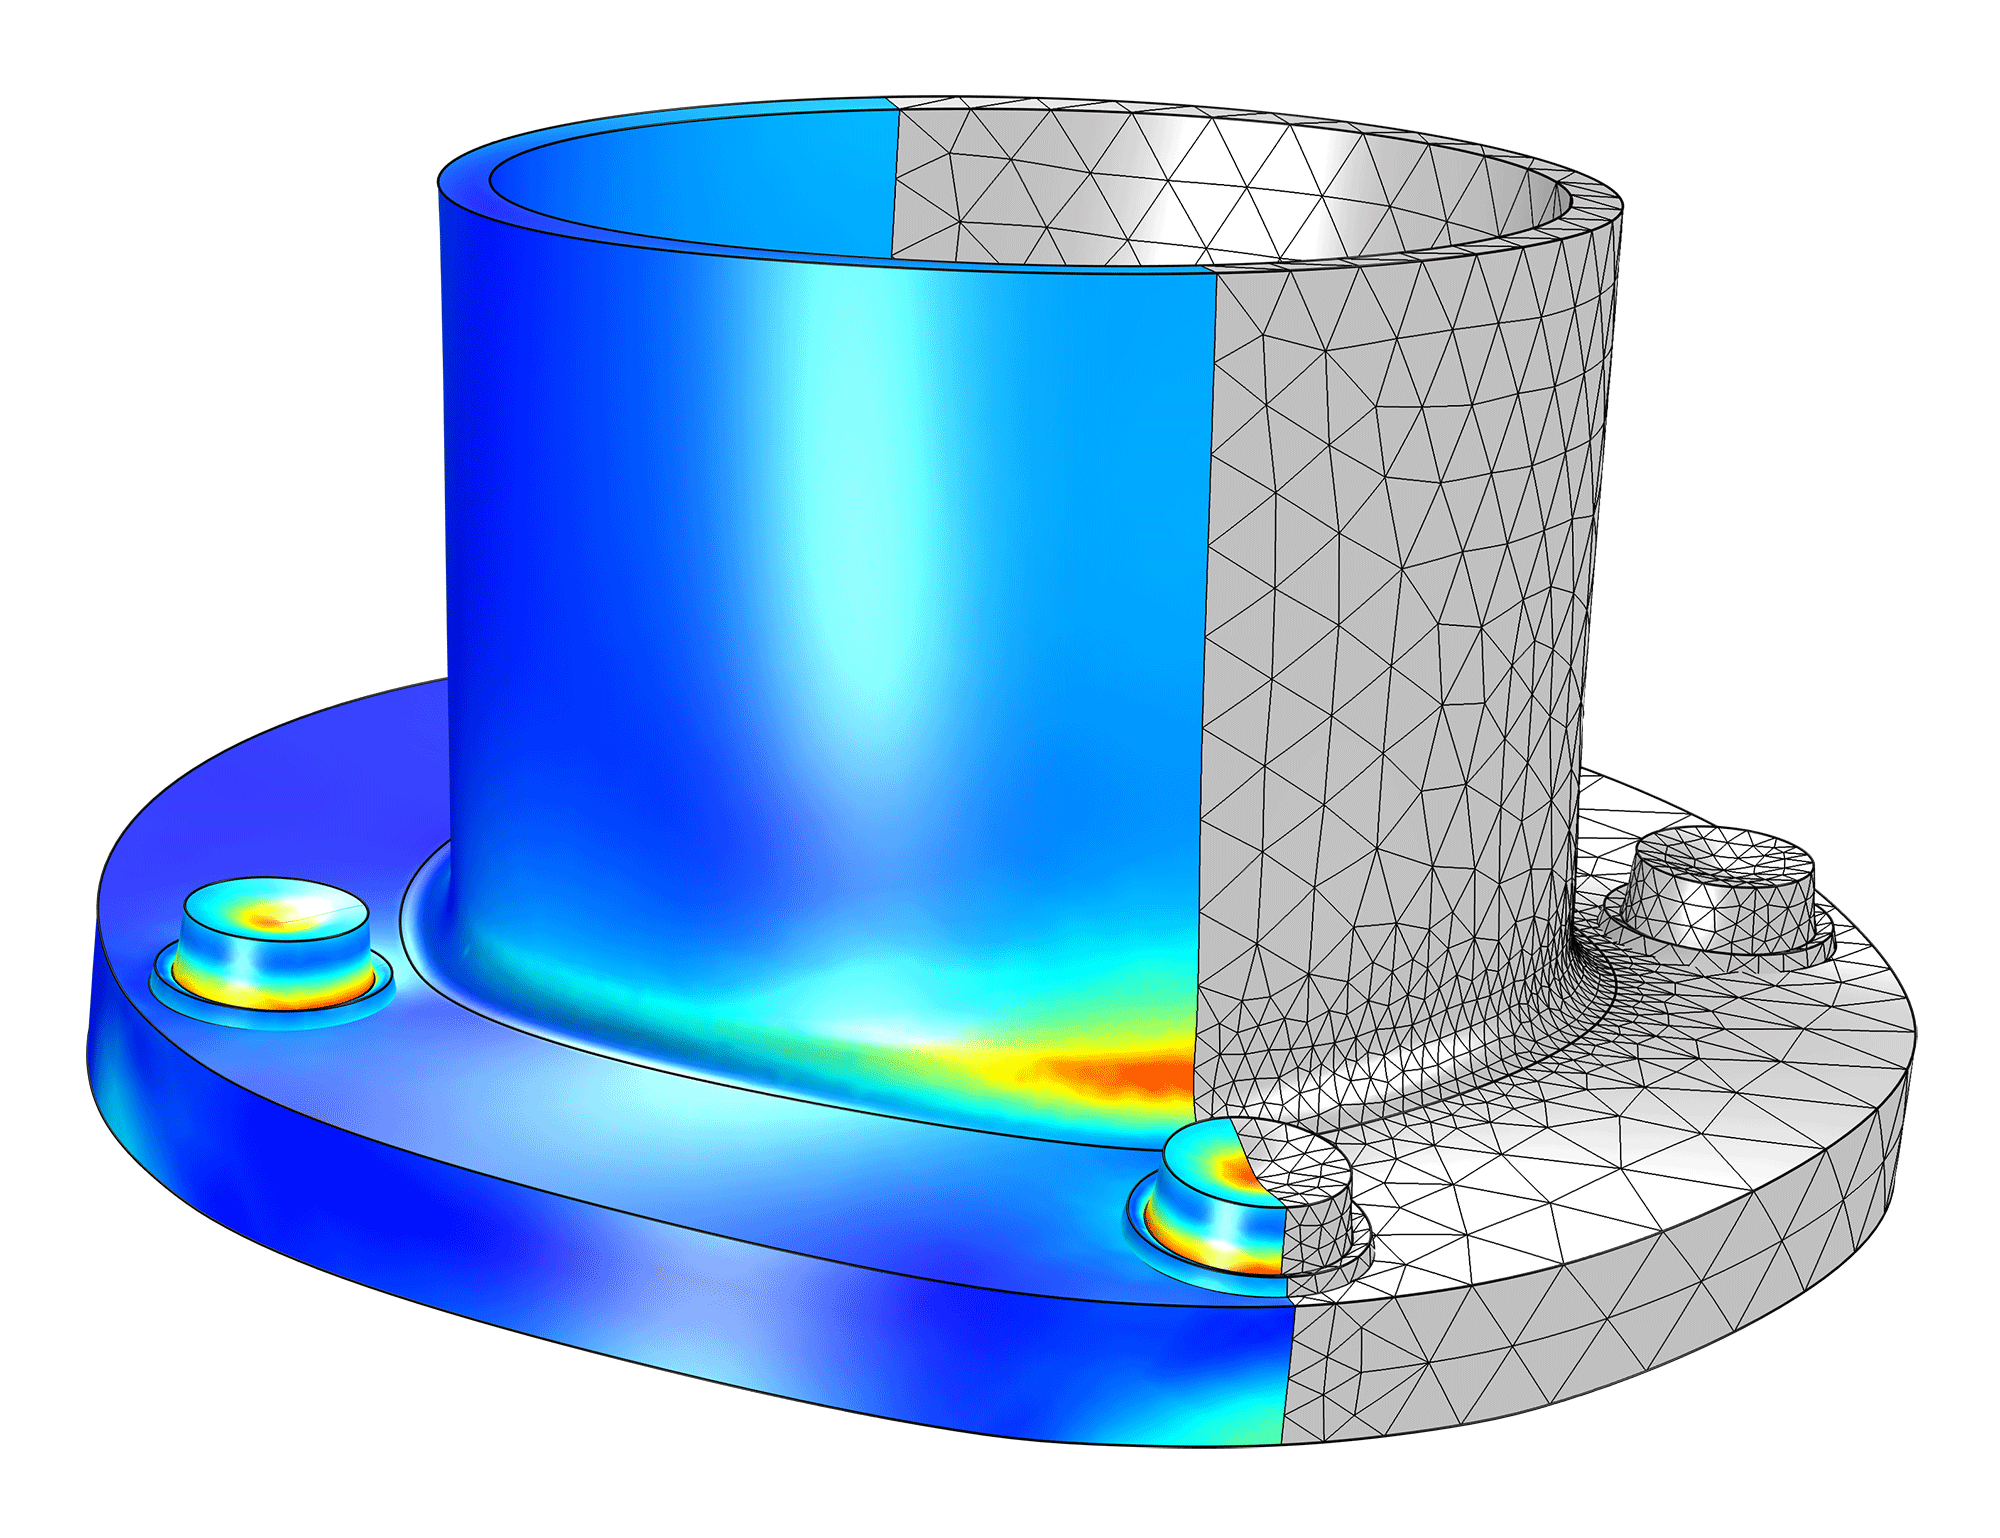
\includegraphics[scale=0.23]{pictures/tube-connection}
  \vfill
  \noindent
  \raggedleft{\Huge\textsf{ME 210: Mechanics of Materials}}
  \vskip\baselineskip
  \noindent
  {\LARGE\textsf{Sappinandana Akamphon}}
\end{titlepage}
\restoregeometry % restores the geometry
\nopagecolor% Use this to restore the color pages to white

\chapter*{Preface}

This reading material is intended for the use in ME210: Mechanics of Materials, both as a teaching and study material. The materials extend those covered in CE202: Engineering Mechanics--Statics by going into more in-depth details, using more rigorous methods, and exploring more advanced case studies.

The topics included in these materials are the review of basic concept of stress-strain, member under axial loads, and member under torsion. However, in each of these, the topics covered will include analysis of composite materials under these loads. Furthermore, analysis of stress transformation will be explained. This will form a basis for the next topic: analysis of member under combined loadings. Finally, the topics will introduce the theories of failure--fracture and yield, fatigue, and buckling.

\vspace{3cm} \hspace{9cm}
Sappinandana Akamphon

\chapter*{Revisions}

\paragraph{July 2011}

Main contents for chapter 1 - 8

\paragraph{March 2012}

Examples for chapters 1-4. Exercises for chapters 1-4.

\paragraph{May 2013}

Examples for chapters 5-7. Exercises for chapters 5-7.

\paragraph{June 2014}

Examples and exercises for chapters 8.

\paragraph{July 2015}

Add sections on curved beam bending, shear flow, and shear center.

\paragraph{March 2016}

Migrated from Microsoft Word to \LaTeX\

\paragraph{April 2017}

Additional graphics for stress transformation, Mohr's circle, combined loadings.

\paragraph{July 2018}

Add more figures to facilitate visualization of examples.

\paragraph{December 2021}

Add shear stress-strain relationship. Add creep and fatigue behaviors.

\tableofcontents

\listoffigures

\listoftables

\mainmatter

%%%%%%%%%%%%%%%%%%%%%%%%%%%%%%%%%%%%%%%%%%%%%%%%%%%%%%%%%%%%%%%%%%%%%%%%%%%%%%%%%%%%%%%%%%%%%%%%%%%%%%%%%%%%%%%%%%%%%%%%%%%%%%%%%%%%%%%%%%%%%%%%%%%%%%%%%%%%%%%%%%%%%%%%%%%%%%

\chapter{Basic Mechanics of Materials Review}
\label{chap: basic mechanics of materials}

The main interest in engineering mechanics of solids is to study the internal resistance of a body under externally applied forces. In earlier statics or dynamics courses, we study the effect of forces on rigid bodies. We may study how they move or how the forces distribute among many members of a structure, but we never study how the force affects each member. In reality, most bodies are deformable, the degrees of which depends on their material properties. In this case, we can still use the equation of equilibrium to determine the internal force acting inside the body.

$$ \sum F = 0 $$
$$ \sum M = 0 $$

\section{General Concepts of Load}

Considering a surface cutting through the body, there can be 2 types of forces and 2 types of moments acting on the surface

\begin{itemize}
  \item Normal force ($F$) acts perpendicular to the surface. This force is developed when there is an external loads pushing or pulling on the surface of the body.
  \item Shear force ($V$) acts in the plane of the surface. It developed when the external forces tends to cause the surface to slide sideways.
  \item Torsional moment or torque ($T$) is developed when the loads tend to twist the segment with respect to another.
  \item Bending moment ($M$) is developed when the loads tend to bend the body about an axis lying within the plane of the surface.
\end{itemize}

\section{Stress}

By definition, stress is the force per unit cross sectional area that it is acting upon. There are two types of stress, depending on the direction the force is acting on the surface

\begin{enumerate}

\item Normal stress: force per unit area acting normal to the surface. It can be expressed mathematically as

\begin{equation}
\sigma  = \mathop {\lim }\limits_{A \to 0} \frac{F}{A}
\end{equation}

\item Shear stress: force per unit area acting tangent to the surface. This component can be expressed mathematically as

  \begin{equation}
    \tau  = \mathop {\lim }\limits_{A \to 0} \frac{V}{A}
  \end{equation}
\end{enumerate}

In the case of shear stress, we can further specify the direction of stress into rectangular components using $x$, $y$, $z$ coordinate axes, with $x$ and $y$ axes in the direction of the in-plane surface and $z$ axis normal to the surface. We can now express the normal stress components as

\begin{equation}
  \sigma _{zz} = {\sigma _z} = \mathop {\lim }\limits_{A \to 0} \frac{{{F_z}}}{A}
\end{equation}

and the two shear stress components as

\begin{equation}
  \arraycolsep=1.4pt\def\arraystretch{2.2}
  \begin{array}{l}
    {\tau _{zx}} = \mathop {\lim }\limits_{A \to 0} \dfrac{F_x}{A} \\
    {\tau _{zy}} = \mathop {\lim }\limits_{A \to 0} \dfrac{F_y}{A}
  \end{array}
\end{equation}

\subsection{Equilibrium Requirement}

Consider an infinitesimal cubic element, illustrated in \cref{fig: 3d-stress-element}, with external forces applied, each of the six faces of the cube will have three components of stress acting on it. If the stress around the point is constant, then we can use equilibrium equation to relate some of the stress components.

\begin{figure}[h]
  \centering
  % 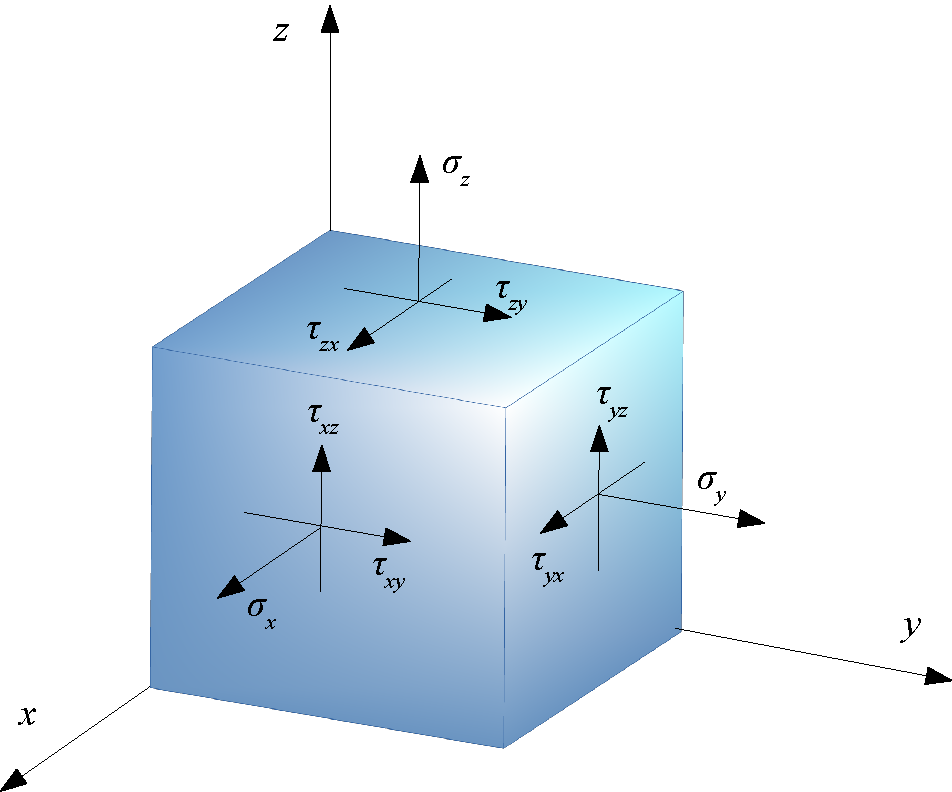
\includegraphics[scale=0.5]{pictures/Static-body-load-analysis/3d-element-stress}
  \tdplotsetmaincoords{70}{110}
  \begin{tikzpicture}[tdplot_main_coords, >=latex]
    \def\length{4}
    \draw [dashed]
    (0,0,0) node(origin){} --++ (\length,0,0) node(x){}
    (origin.center) --++ (0,\length,0) node(y){}
    (origin.center) --++ (0,0,\length) node(z){};
    \draw [thin, left color=LightSkyBlue, right color=LightSkyBlue!\length0]
    (x.center) --++ (0,0,\length) --++ (0,\length,0) --++ (0,0,-\length) -- cycle;
    \draw [thin, right color=LightSkyBlue, left color=LightSkyBlue!\length0]
    (y.center) --++ (0,0,\length) --++ (\length,0,0) --++ (0,0,-\length) -- cycle;
    \draw [thin, top color=LightSkyBlue, bottom color=LightSkyBlue!\length0]
    (z.center) --++ (\length,0,0) --++ (0,\length,0) --++ (-\length,0,0) -- cycle;
    \draw [dashed, ->] (x.center) --++ (\length/3,0,0) node[below left]{$x$};
    \draw [dashed, ->] (y.center) --++ (0,\length/3,0) node[below right]{$y$} ;
    \draw [dashed, ->] (z.center) --++ (0,0,1) node[above]{$z$};
    % shear stresses
    \draw [->, ultra thick] (x.center) ++ (0,\length/2,\length/3) --++ (0,0,\length/3) node[above]{$\tau_{xz}$};
    \draw [->, ultra thick] (x.center) ++ (0,\length/3,\length/2) --++ (0,\length/3,0) node[right]{$\tau_{xy}$};
    \draw [->, ultra thick] (y.center) ++ (\length/2,0,\length/3) --++ (0,0,\length/3) node[above]{$\tau_{yz}$};
    \draw [->, ultra thick] (y.center) ++ (\length/3,0,\length/2) --++ (\length/3,0,0) node[left]{$\tau_{yx}$};
    \draw [->, ultra thick] (z.center) ++ (\length/2,\length/3,0) --++ (0,\length/3,0) node[right]{$\tau_{zy}$};
    \draw [->, ultra thick] (z.center) ++ (\length/3,\length/2,0) --++ (\length/3,0,0) node[below left]{$\tau_{zx}$};
    % normal stresses
    \draw [->, ultra thick] (x.center) ++ (0,\length/2,\length/2) --++ (\length/2,0,0) node[left]{$\sigma_{x}$};
    \draw [->, ultra thick] (y.center) ++ (\length/2,0,\length/2) --++ (0,\length/2,0) node[right]{$\sigma_{y}$};
    \draw [->, ultra thick] (z.center) ++ (\length/2,\length/2,0) --++ (0,0,\length/2) node[above]{$\sigma_{z}$};
  \end{tikzpicture}
  \caption{Stresses on a three-dimensional element when considering a static equilibrium}
  \label{fig: 3d-stress-element}
\end{figure}
  
\paragraph{Normal Stress Components}

If we apply the equation of force equilibrium in the $x$ direction, then

\begin{equation}
  \arraycolsep=1.4pt\def\arraystretch{1.5}
  \begin{array}{c}
    \sigma_x(\Delta y\Delta z) + \sigma_x^\prime(\Delta y\Delta z) = 0\\
    \sigma_x =  - \sigma_x^\prime
  \end{array}
\end{equation}

We can similarly prove that $\sigma_y = \sigma_{y ^\prime}$ and $\sigma_z = \sigma_z ^\prime$. Therefore, for a constant state of stress, each of the three normal stress components must be equal in magnitude but opposite in direction.

\paragraph{Shear Stress Components}

In similar fashion, the shear stresses on opposite faces are of the same magnitude but in opposite direction.
The force equilibrium in the $x$ direction gives

\begin{equation}
  \arraycolsep=1.4pt\def\arraystretch{1.5}
  \begin{array}{c}
    {\tau _{yx}}(\Delta y\Delta z) + {\tau_{yx}^\prime}(\Delta y\Delta z) = 0\\
    {\tau _{yx}} =  - {\tau_{yx}^\prime}
  \end{array}
\end{equation}

If we consider a pair of shear stresses loading on the element, the moment equilibrium about the $z$ direction gives

\begin{equation}
  \arraycolsep=1.4pt\def\arraystretch{1.5}
  \begin{array}{c}
    {\tau _{xy}}(\Delta y\Delta z)\Delta x - {\tau _{yx}}(\Delta x\Delta z)\Delta y = 0\\
    {\tau _{xy}} = {\tau _{yx}}
  \end{array}
\end{equation}

\section{Strain}

In order to describe deformation by changes in the length or by the changes in angles of the element, we will need to develop the concept of strain. As in stresses, there are two types of strain.

\begin{figure}[h]
  \centering
  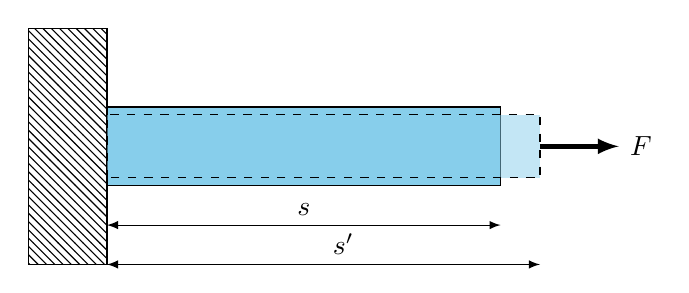
\begin{tikzpicture}
    \draw[pattern=north west lines] (-1,-1) rectangle (0,2);
    \draw[fill=SkyBlue] (0,0) rectangle (5,1);
    \draw[fill=SkyBlue, fill opacity=0.5, dashed] (0,0.1) rectangle (5.5,0.9);
    \draw[->,ultra thick] (5.5,0.5) -- (6.5,0.5) node[right]{$F$};
    \draw[<->] (0,-0.5) -- (2.5,-0.5) node[above]{$s$} -- (5,-0.5);
    \draw[<->] (0,-1) -- (3,-1) node[above]{$s^\prime$} -- (5.5,-1);
  \end{tikzpicture}
  \caption{Element elongation under tensile normal strain.}
\end{figure}

\paragraph{Normal strain} The change in the length of a line segment per unit length, whether elongation or contraction, is called normal strain. For example, consider the line AB which is contained within an undeformed body with length $s$. During its deformation, points A and B move to point A’ and B’ and the line becomes a curve having the length $s^\prime$. The average normal strain becomes

\begin{equation}
  \varepsilon_{avg} = \frac{s^\prime - s}{s}
\end{equation}

If the normal strain is known, we can use this equation to find the final length of the line segment after it is deformed. We have

\begin{equation}
  s^\prime = (1 + \varepsilon_{avg})s
\end{equation}

Therefore, strain is positive when the line elongates and is negative when the line contracts.

\paragraph{Shear Strain} The change in angle that occurs between two line segments that were originally perpendicular is referred to as shear strain. This angle is denoted by and is measured in radians. Consider the same cubic element with shear stress couple applied in the $xy$-plane. The angle made by the original $x$ and $y$ axes is $90\degree$. After the deformation, the angle is changed by $\theta$. The shear strain in the plane, $\gamma_{xy}$, can be defined as 

\begin{figure}[h]
  \centering
  % 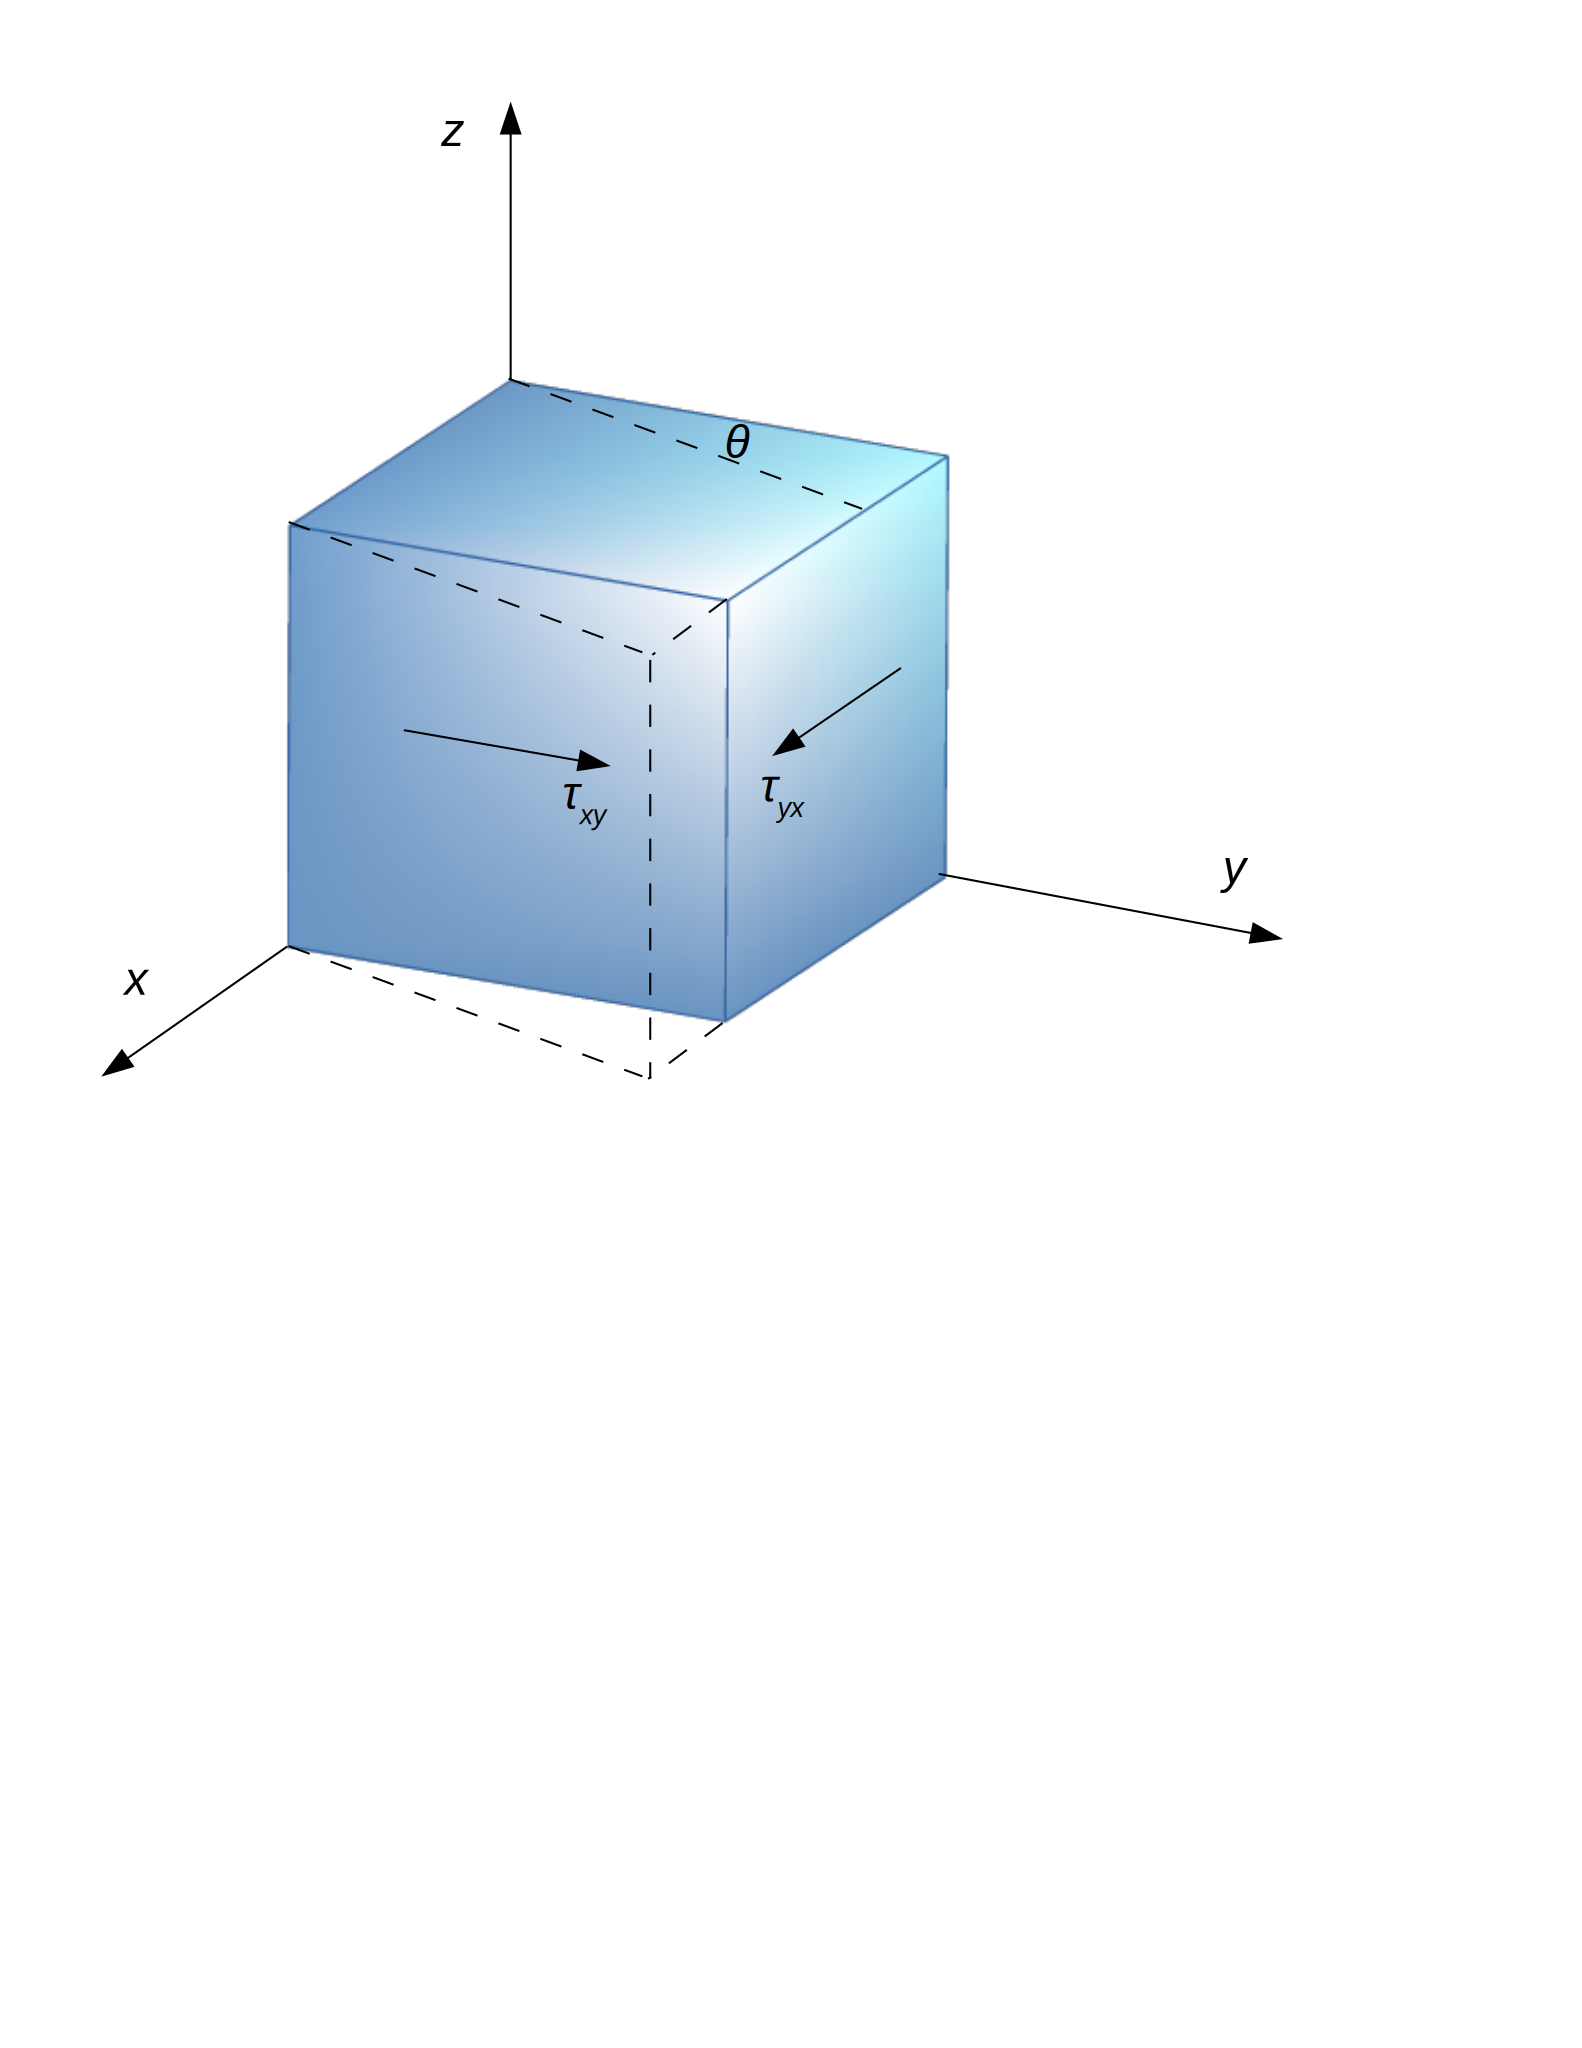
\includegraphics[scale=0.5]{pictures/Static-body-load-analysis/3d-shear-deformation}
  \tdplotsetmaincoords{70}{110}
  \begin{tikzpicture}[tdplot_main_coords, >=latex]
    \draw [dashed]
    (0,0,0) node(origin){} --++ (3,0,0) node(x){}
    (origin.center) --++ (0,3,0) node(y){}
    (origin.center) --++ (0,0,3) node(z){};
    \draw [thin, left color=LightSkyBlue, right color=LightSkyBlue!30]
    (x.center) --++ (0,0,3) --++ (0,3,0) --++ (0,0,-3) -- cycle;
    \draw [thin, right color=LightSkyBlue, left color=LightSkyBlue!30]
    (y.center) --++ (0,0,3) --++ (3,0,0) --++ (0,0,-3) -- cycle;
    \draw [thin, top color=LightSkyBlue, bottom color=LightSkyBlue!30]
    (z.center) --++ (3,0,0) --++ (0,3,0) --++ (-3,0,0) -- cycle;
    \draw [dashed, ->] (x.center) --++ (1,0,0) node[below left]{$x$};
    \draw [dashed, ->] (y.center) --++ (0,1,0) node[below right]{$y$} ;
    \draw [dashed, ->] (z.center) --++ (0,0,1) node[above]{$z$};
    % deformed shape
    \draw [dashed]
    (z.center) --++ (1,3,0) node[above left]{$\theta$} --++ (3,0,0)
    (x.center) ++ (0,0,3) --++ (1,3,0) --++ (0,0,-3)
    (x.center) --++ (1,3,0) --++ (-1,0,0);
    % shear stresses
    \draw [->, ultra thick] (x.center) ++ (0,1,1.5) --++ (0,1,0) node[midway, above]{$\tau_{xy}$};
    \draw [->, ultra thick] (y.center) ++ (1,0,1.5) --++ (1,0,0) node[midway, above]{$\tau_{yx}$};
  \end{tikzpicture}
  \caption{3-dimensional element under shear deformation.}
  \label{fig: 3d shear deformation}
\end{figure}

\begin{equation}
  \gamma_{xy} = \mathop {\lim} \limits_{y \to 0} \frac{{dx}}{y} = \tan \theta  \approx \theta
\end{equation}
 
\paragraph{Cartesian Strain Components}

Using the above definition of normal and shear strains, we will now show how it can be used to describe the deformation in a body. Consider an infinitesimal element of dimension that is located near a point in the body. The deformed shape of the element is a parallelepiped, assuming that very small line segments will remain relatively straight after the deformation. The approximate lengths of the sides of the parallelepiped are  $(1 + {\varepsilon _x})\Delta x$, $(1 + {\varepsilon _y})\Delta y$, and $(1 + {\varepsilon _z})\Delta z$ and the approximate angles between the sides are $(\pi /2) - {\gamma _{xy}}$, $(\pi /2) - {\gamma _{yz}}$, and $(\pi /2) - {\gamma _{zx}}$. Notice that the normal strains cause a change in the volume of the element, while the shear strains cause a change in its shape.

\section{Mechanical Properties of Materials}

\subsection{Tension and Compression Test}

Material behaviors must be determined by experiment. In order to understand how a material responds to external loads, one of the most important tests is the \emph{tension or compression test}. Though many properties of a material can be determined by this test, it is mainly used to determine the relationship between the average stress and average strain of a material.

To perform a tension or compression test, a specimen of the material is made into a standard shape and size--typically a cylinder with enlardged ends to ensure failure will occur along the middle of its length. Measurements are taken of both its initial cross sectional area and length. The specimen is then mounted on a test machine which is used to stretch the material until it fails. During the test, the machine takes frequent records of the applied load and the elongation of the specimen.

\subsection{Stress-Strain Diagram}

In order to for the load and deformation response from the tension or compression test to be universally useful, not just for the tested specimen cross-sectional area and length, we must normalize the applied force and deformation of the specimen. We can do so by dividing the applied force with the specimen cross-sectional area, and dividing the deformation by its original length, giving us a stress-strain diagram (rather than a force-deformation diagram).

While the actual stress-strain diagrams of different materials can be vastly different, we may discuss some of their common characteristics, illustrated in \cref{fig: stress-strain diagram}

\begin{figure}[h]
  \centering
  % 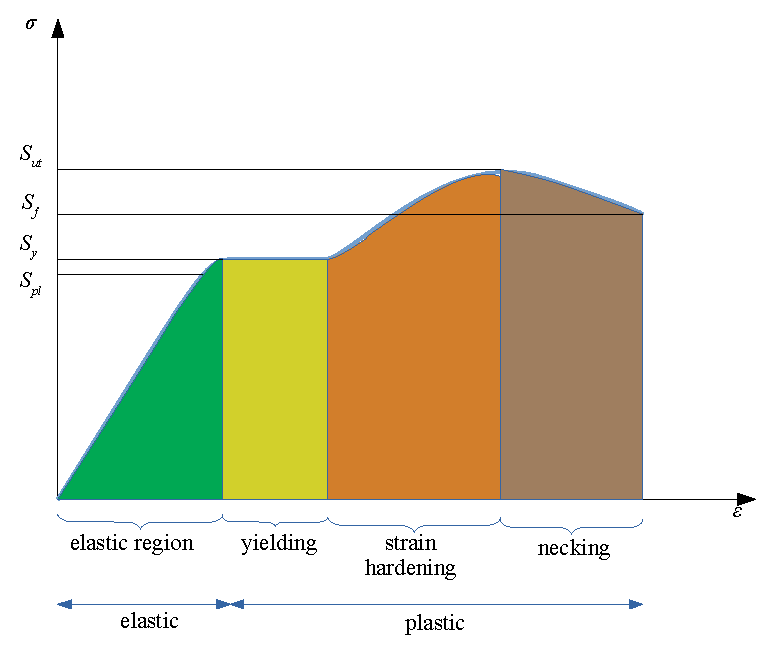
\includegraphics[scale=1]{pictures/Basic-material-behavior/stress-strain-diagram} \\
  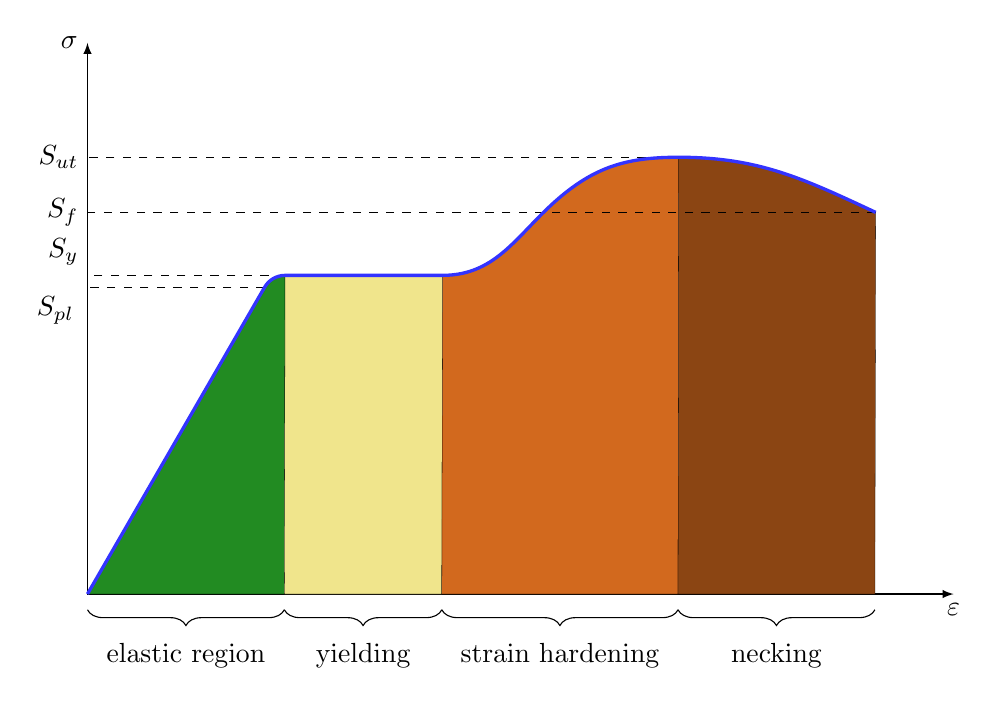
\begin{tikzpicture}[>=latex]
    % axes
    \draw [<->] (0,7) node[left]{$\sigma$} --++ (-90:7) node(O){} --++ (0:11) node[below]{$\varepsilon$};
    % braces
    \draw [decorate, decoration={brace, mirror, amplitude=2mm}] (O.center) ++ (-90:0.2) --++ (0:2.5) node(B){} node[midway, below, yshift=-3mm]{elastic region};
    \draw [decorate, decoration={brace, mirror, amplitude=2mm}] (B.center) --++ (0:2) node(C){} node[midway, below, yshift=-3mm]{yielding};
    \draw [decorate, decoration={brace, mirror, amplitude=2mm}] (C.center) --++ (0:3) node(D){} node[midway, below, yshift=-3mm]{strain hardening};
    \draw [decorate, decoration={brace, mirror, amplitude=2mm}] (D.center) --++ (0:2.5) node(E){} node[midway, below, yshift=-3mm]{necking};
    % area under curve
    \draw [ultra thin, fill=ForestGreen] (B.center) ++ (90:0.2) node(F){} -- (O.center) --++ (60:4.5) node(pl){} arc (150:90:0.3) node(G){} -- cycle;
    \draw [ultra thin, fill=Khaki] (C.center) ++ (90:0.2) node(H){} -- (F.center) -- (G.center) --++ (0:2) node(I){} -- cycle;
    \draw [ultra thin, fill=Chocolate] (D.center) ++ (90:0.2) node(J){} -- (H.center) -- (I.center) to [out=0, in=-140] ++(1.5,1) to [out=40,in=180] ++(1.5,0.5) node(K){} -- cycle;
    \draw [ultra thin, fill=SaddleBrown] (E.center) ++ (90:0.2) node(L){} -- (J.center) -- (K.center) to [out=0, in=155] ++(2.5,-0.7) node(M){} -- cycle;
    % stress indicators
    \draw [dashed] (pl.center) -- +(180:2.3) node[below left]{$S_{pl}$};
    \draw [dashed] (G.center) -- +(180:2.5) node[above left]{$S_{y}$};
    \draw [dashed] (K.center) -- +(180:7.5) node[left]{$S_{ut}$};
    \draw [dashed] (M.center) -- +(180:10) node[left]{$S_{f}$};
    % actual curve
    \draw [very thick, Blue!80](O.center) -- (pl.center) arc (150:90:0.3) -- (I.center) to [out=0, in=-140] ++(1.5,1) to [out=40,in=180] ++(1.5,0.5) to [out=0, in=155] ++(2.5,-0.7);
  \end{tikzpicture}
  \caption{A general stress-strain diagram obtained from a tensile test.}
  \label{fig: stress-strain diagram}
\end{figure}

\paragraph{Elastic Behavior:} occurs when the stress-strain relationship remains linear, where the strain is still in the green region. The upper lilmit stress of this linear relationship is called the \emph{proportionality limit}, $S_{pl}$. If the applied stress exceeds this value, the curve no longer remains linear and usually curves down and flattens out. This continues until the \emph{elastic limit} below which any deformation occured due to this stress disappears when the stress is removed. For most materials, this elastic limit can be difficult to determine and distinguish from the proportionality limit.

\paragraph{Yielding:} Just beyond the elastic limit is the stress that will cause a permanent deformation in the specimen, also called the \emph{yield stress}, $S_y$. The permanent deformation that occurs is called \emph{plastic deformation}. During this period, the specimen will continue to elongate without any increase in the load. This is referred to as being \emph{perfectly plastic}.

\paragraph{Strain Hardening:} After yielding has ended, additional load can be supported by the specimen although the slope of the stress-strain diagram will decrease until it reaches the maximum stress, referred to as the \emph{ultimate stress}, $S_{ut}$. The rise in the curve after yielding is called \emph{strain hardening} and is denoted by the area in light brown.

\paragraph{Necking:} After yielding, the cross-sectional area of the specimen will continue to decrease, albeit uniformly throughout. However, when the stress is close the ultimate stress, the decrease in cross section will become localized as the specimen continues to elongate. The stress-strain curve beyond the ultimate stress usually curves downward, finally reaching the \emph{fracture stress}, $S_f$, when the specimen completely separates.

\subsection{Ductile and Brittle Materials}

Materials can be categorized as either ductile or brittle, depending on their stress-strain characteristics.

\begin{marginfigure}
  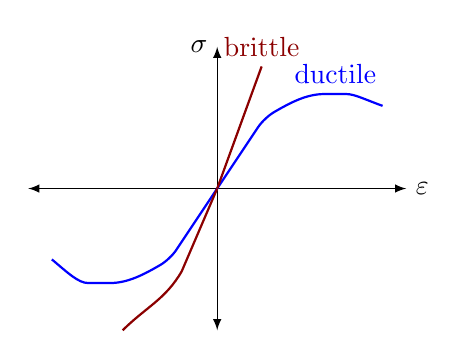
\begin{tikzpicture}[scale=0.3]
    %\draw (-6,-5) grid (6,5);
    \draw[<->] (0,-6) -- (0,6) node[left]{$\sigma$};
    \draw[<->] (-8,0) -- (8,0) node[right]{$\varepsilon$};
    \draw[thick, Blue, rounded corners] (0,0) to (2,3) to [out=30,in=-180] (5,4) node[above]{ductile} to [out=0,in=160] (7,3.5);
    \draw[thick, DarkRed] (0,0) --++ (70:5.5) node[above]{brittle};
    \draw[thick, Blue, rounded corners] (0,0) to (-2,-3) to [out=210,in=0] (-5,-4) to [out=180,in=-40] (-7,-3);
    \draw[thick, DarkRed] (0,0) to (-1.5,-3.5) to [out=-120,in=45] (-4,-6);
  \end{tikzpicture}
  \caption{Typical stress-strain curves for ductile and brittle materials.}
\end{marginfigure}

\subsubsection{Ductile Materials}

Materials that can withstand large amount of strains before fracture are called \emph{ductile materials}. Ductile materials are typically the materials of choice for component design because they are capable of absorbing shock and energy. Even if they are loaded excessively, they will undergo large deformation before failure.

One method of defining the ductility of a material is by reporting its elongation at failure, for which the formula is

\begin{equation}
  \text{\% elongation} = \frac{L_f - L_0}{L_0} \times 100\%
\end{equation}

For a typical mild steel specimen, this value is around 38\%.

Another indicator of material ductility is its cross-sectional area reduction percentage at failure, for which the formula is

\begin{equation}
  \text{\% reduction of area} = \frac{A_0 - A_f}{A_0} \times 100\%
\end{equation}

Mild steel typically has a typical reduction of area at 60\%.

It is important to note that, beside steel, most ductile materials do not yield at constant loads. This makes defining an actual yield stress difficult. In this case, the yield stress can be obtained by the \emph{offset method} in which a line parallel to the elastic region of the stress-strain curve of a material is drawn from where strain is equal to 0.2\%. The point where this line intersects with the curve is defined as the yield stress.


\subsubsection{Brittle Materials}

Materials that shows very small or no yielding at all before failure is called \emph{brittle materials}. Grey cast iron is the usual example.

Brittle materials in general shows much higher resistance to compressive loading than tensile loading. Concrete, another typical brittle material, has the maximum tensile strength of only 2.8 MPa, but has the maximum compressive strength of 35 MPa.

In general it can be said that most materials can exhibit both ductile and brittle behavior. At high carbon content or very low temperature, steel tends to become more brittle. At higher temperature, most brittle materials become more ductile.

\subsection{Strain Energy}

When a material is deformed, it stores energy internally under its deformed state. Since this energy is related to the strains in the material, it is called \emph{strain energy}. To determine this energy, consider a volume under a tensile test for which force $F = \sigma A = \sigma xy$. The force increases linearly from when there is no deformation to its final magnitude $F$, hence the average force over the range of deformation is $F/2$. The work done by this force then is $F/2*\varepsilon z$. Assuming that there is no loss from the externally applied force to the internal strain energy in the form of heat, the strain energy is equal to the external work, which is $U = \sigma\varepsilon xyz/2$. Since $V = xyz$ is the original volume, we can write that $U = \frac{1}{2}\sigma\varepsilon V$. In another word, the strain energy density $u$, the strain energy per volume is

\begin{align}
  \label{eq: strain energy density}
  u = \frac{1}{2}\sigma\varepsilon
\end{align}

For most engineering materials of interest, their behaviors are usually \emph{linear elastic}, and thus we can express the strain energy density in terms of uniaxial stress as

\begin{align}
  \label{eq: strain energy density - linear elastic}
  u = \frac{1}{2}\frac{\sigma^2}{E}
\end{align}

\paragraph{Modulus of Resilience} When the stress reaches the propoortional limit, the corresponding strain energy is referred to as the \emph{modulus of resilience}, expressed as

\begin{align}
  \label{eq: modulus of resilience}
  u_r = \frac{1}{2}\sigma_{pl}\varepsilon_{pl} = \frac{1}{2}\frac{\sigma_{pl}^2}{E}
\end{align}

This represents the amount of energy the material can absorb without any permanent deformation.

\begin{figure}[H]
  \centering
  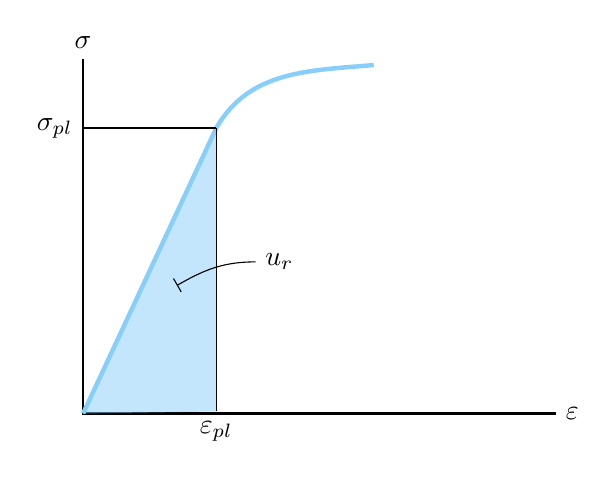
\begin{tikzpicture}
    \draw [thick] (0,4.5) node[above]{$\sigma$} --++ (-90:4.5) --++ (0:6) node[right]{$\varepsilon$};
    \draw [ultra thick, LightSkyBlue] (0,0) --++ (65:4) node(pl){} to[out=60, in=185] +(2,0.8);
    \path[fill=LightSkyBlue, fill opacity=0.5] (0,0) -- (pl.center) --++ (-90:3.6) -- cycle;
    \draw [|-] (pl) ++ (-0.5,-2) to[out=30,in=180] +(1,0.3) node[right]{$u_r$};
    \draw (pl.center) --++ (-90:3.6) node[below]{$\varepsilon_{pl}$};
    \draw (pl.center) --++ (180:1.7) node[left]{$\sigma_{pl}$};
  \end{tikzpicture}
  \caption{Modulus of resilience, $u_r$}
  \label{fig: modulus of toughness}
\end{figure}

\paragraph{Modulus of Toughness} Another important property of a material the modulus of toughness $u_t$. This quantity represents the entire area under the stress-strain diagram, indicating the strain energy density required for the maeterial to fracture. This property is important when designing members that may be overloaded.

\begin{figure}[H]
  \centering
  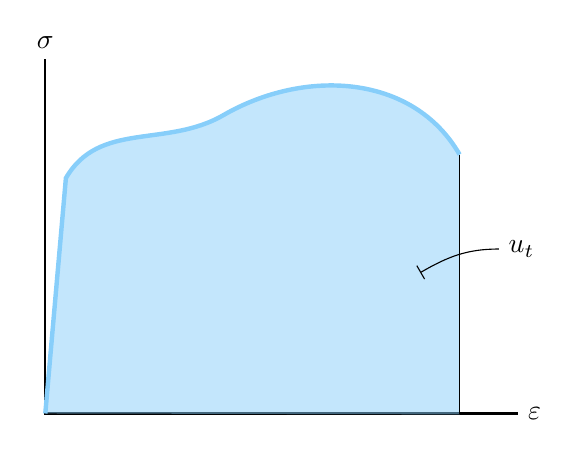
\begin{tikzpicture}
    \draw [thick] (0,4.5) node[above]{$\sigma$} --++ (-90:4.5) --++ (0:6) node[right]{$\varepsilon$};
    \draw [ultra thick, LightSkyBlue] (0,0) --++ (85:3) node(pl){} to[out=60, in=210] ++(2,0.8) to[out=30,in=120] ++(3,-0.5);
    \path[fill=LightSkyBlue, fill opacity=0.5] (0,0) -- (pl.center) to[out=60, in=210] ++(2,0.8) to[out=30,in=120] ++(3,-0.5) node(ut){} --++ (-90:3.30) -- cycle;
    \draw (ut.center) --++ (-90:3.30);
    \draw [|-] (ut) ++ (-0.5,-1.5) to[out=30,in=180] ++(1,0.3) node[right]{$u_t$};
  \end{tikzpicture}
  \caption{Modulus of toughness, $u_t$}
  \label{fig: modulus of resilience}
\end{figure}

\subsection{Hooke’s Law in One Dimension}

Since the stress-strain relationship for most engineering materials exhibit a linear relationship between stress and strain within the elastic regime, an increase in stress causes a proportional increase in strain. This fact was discovered by Robert Hooke in 1676 and is known as Hooke’s law. It can be expressed mathematically as

\begin{equation}
  \sigma  = E\varepsilon
\end{equation}

Here $E$ represents the constant of proportionality, which is called the modulus of elasticity or Young’s modulus.

\subsection{Poisson’s Ratio}

When a deformable body is subjected to an axial tensile force, not only does it elongate but it also contracts laterally. A French scientist S. D. Poisson found that the ratio between lateral and the longitudinal strains are always constant in the elastic regime. This constant is referred to as Poisson’s ratio, $\nu$, defined as

\begin{equation}
  \nu  =  - \frac{\varepsilon _{lat}}{\varepsilon _{long}}
\end{equation}
  
Notice the negative sign here since longitudinal elongation causes lateral contraction, and vice versa, as illustrated in \cref{fig: poisson's ratio}. It is also important to note that Poisson’s ratio has no unit, i.e. it is dimensionless. 

\begin{figure}[h]
  \centering
  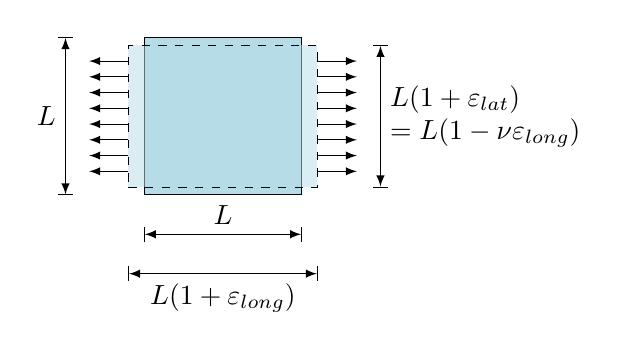
\begin{tikzpicture}[>=latex]
    \node [draw, rectangle, minimum height=2cm, minimum width=2cm, fill=LightBlue!90, inner sep=0](A){};
    \node [draw, dashed, rectangle, minimum height=1.8cm, minimum width=2.4cm, fill=LightBlue!90, fill opacity=0.5, inner sep=0](B){};
    \foreach \x in {1,...,8} {
      \draw [->] (1.2, 0.9-0.2*\x) --++ (0:0.5);
      \draw [->] (-1.2, 0.9-0.2*\x) --++ (180:0.5);
    }

    \node at (A.west) [yshift=-1.5cm](C){};
    \node at (A.east) [yshift=-1.5cm](D){};

    \node at (B.west) [yshift=-2cm](E){};
    \node at (B.east) [yshift=-2cm](F){};

    \draw [|<->|] (C.center) -- (D.center) node[midway,above]{$L$};
    \draw [|<->|] (E.center) -- (F.center) node[midway,below]{$L(1+\varepsilon_{long})$};

    \node at (A.north) [xshift=-2cm](G){};
    \node at (A.south) [xshift=-2cm](H){};

    \node at (B.north) [xshift=2cm](I){};
    \node at (B.south) [xshift=2cm](J){};

    \draw [|<->|] (G.center) -- (H.center) node[midway,left]{$L$};
    \draw [|<->|] (I.center) -- (J.center) node[text width=2.7cm,midway,right]{$L(1+\varepsilon_{lat})$ \\
      $= L(1-\nu\varepsilon_{long})$};
  \end{tikzpicture}
  \caption{The effect of Poisson's ratio in an element under uniaxial loading.}
  \label{fig: poisson's ratio}
\end{figure}

Poisson's ratios for various common materials are tabulated in \cref{table: poisson's of materials}. Note that the ratios are listed in descending order, and that they stay between 0 and 0.5. Why is that? Can you have $\nu > 0.5$? What about $\nu < 0$?

\begin{margintable}
  \centering
  \caption{Poisson's ratio of various engineering materials.}
  \label{table: poisson's of materials}
  {\renewcommand\arraystretch{1.2}
    \begin{tabular}{ll}
      \toprule
      Material        & Poisson's ratio \\
      \midrule
      rubber          & 0.4999          \\
      gold            & 0.42 - 0.44       \\
      saturated clay  & 0.40 - 0.49       \\
      magnesium       & 0.252 - 0.289     \\
      titanium        & 0.265 - 0.34      \\
      copper          & 0.33            \\
      aluminium-alloy & 0.32            \\
      clay            & 0.30 - 0.45       \\
      stainless steel & 0.30 - 0.31       \\
      steel           & 0.27 - 0.30       \\
      cast iron       & 0.21 - 0.26       \\
      sand            & 0.20 - 0.45       \\
      concrete        & 0.1 - 0.2         \\
      glass           & 0.18 - 0.3        \\
      foam            & 0.10 - 0.50       \\
      cork            & 0               \\
      \bottomrule
    \end{tabular}}
\end{margintable}

\begin{example}
A thin rubber sheet of material with dimension 2 m x 4 m ($W \times L$) has $E$ = 200 MPa. A normal stress of 20 MPa is applied along the width of the sheet. What is the change in area of the material once the stress is applied. Assume the material has $\nu$ = 0.25
\end{example}

\begin{solution}
To determine the change in area, we need to find the dimension of the length and width of the sheet after the application of stress. First, we have to determine the strain in the longitudinal direction by applying Hooke’s law, from which we have

\begin{align*}
  \sigma _{long} &= E{\varepsilon _{long}} \\
  \varepsilon _{long} &= \frac{20 \times 10^6 \text{ Pa}}{200 \times 10^6 \text{ Pa}} = 0.1
\end{align*}

From the strain, we can calculate the final length by

\[{L_f} = (1 + {\varepsilon _{long}}){L} = (1 + 0.1)4 = 2.2 \text{ m}\]

We can find the transversal strain by using the Poisson’s ratio and calculate the final width by

\begin{align*}
  W_{f} = (1 + {\varepsilon _{width}})W & = (1 - \nu {\varepsilon _{long}})W \\ 
                                        & = (1 - (0.25)(0.1))(4) \\ 
                                        &= 3.9 \text{ m} 
\end{align*}

Therefore, the total area change is

\[\begin{gathered}
  \Delta A = (2.2)(3.9) - (2)(4) \\ 
   = 0.58 \text{ m}^2 \\ 
\end{gathered} \]
\end{solution}

\subsection{Shear stress-shear strain relationship}

Much like the way there is a relationship between normal stress and normal strain in most engineering materials, shear stress and shear strain also exhibit relationship which can be illustrated in \cref{fig: shear stress-strain diagram}

\begin{marginfigure}
  \begin{tikzpicture}[>=latex, scale=0.8]
    % axes
    \draw [<->] (0,5) node[left]{$\sigma$} --++ (-90:5) node(O){} --++ (0:5) node[below]{$\varepsilon$};
    % curve
    \draw [very thick, Blue!80](O.center) --++ (1,2.5) node(pl){} to[out=60, in=180] ++ (2,1) node(u){} to[out=0, in=145] ++ (1.5,-0.4) node(f){};
    \draw [dashed] (pl.center) --++ (180:1) node[left]{$\tau_{pl}$};
    \draw [dashed] (u.center) --++ (180:3) node[left]{$\tau_{u}$};
    \draw [dashed] (f.center) --++ (180:4.5) node[left]{$\tau_{f}$};
  \end{tikzpicture}
  \caption{A general shear stress-shear strain diagram from a torsion test}
  \label{fig: shear stress-strain diagram}
\end{marginfigure}

This relationship can be studied using specimens of thin tubes under torsion. At first, the material with exhibit linear-elastic behavior up until its \emph{proportionality limit}, $\tau_{pl}$. Afterwards, strain hardening occurs until the material reaches its maximum shear stress limit, aka its \emph{ultimate shear stress}, $\tau_{u}$. Finally, the material will lose its shear strength until it reaches the point of fracture at $\tau_{f}$.

\begin{equation}
  \tau  = G\gamma
\end{equation}

$G$ is called the shear modulus of elasticity and has the same unit as Young’s modulus. It can also be shown, later in ..., hat $G$, $E$, and $\nu$ are related by the equation

\begin{equation}
  \label{eq: young and shear}
  G = \frac{E}{2(1 + \nu)}
\end{equation}

\section{Thermal effect}

A change in temperature can cause a material to change its dimensions. If the temperature increases, generally a material expands, whereas if the temperature decreases, the material will contract. Ordinarily this expansion or contraction is linearly related to the temperature increase or decrease that occurs. If the material is homogeneous and isotropic, it has been found that the deformation of a part having length $L$ can be calculated using the formula

\begin{equation}
  \delta _T = \alpha \Delta TL
\end{equation}

where $\alpha$ is a property of a material, referred to as the linear coefficient of thermal expansion, measuring strain per degree temperature, $\Delta T$ is the change in temperature of the part, $L$ is the original length of the member, and $\delta T$ is the change in length of the part. However, if the change in temperature varies throughout the length of the part so that or if varies along the length, then the equation becomes

\begin{equation}
  \delta _T = \int_0^L \alpha \Delta Tdx
\end{equation}

Without any constraint, the change in length of the part can be computed using the given equations. However, if the expansion or contraction is restrained by supports, it will produce thermal stress in the part because it cannot deform freely.

\begin{example}
  
  A rubber bar of original length $L$ is stretched and glued between two walls. After that the bar is heated from its initial temperature $T_0$ to $T$ at which point there is no longer any remaining stress inside the bar. What is the distance between the two walls? Assume the material has modulus of elasticity $E$ and coefficient of thermal expansion $\alpha$.
  
  \begin{figure}[H]
    \centering
    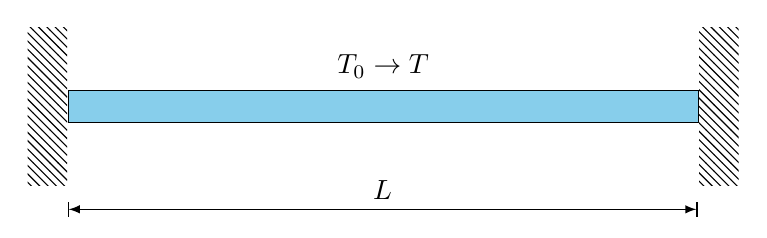
\begin{tikzpicture}
      % \path[fill=white] (-5,-2) rectangle (5,2);
      % \draw (-5,-2) grid (5,2);
      \node [draw, fill=SkyBlue, minimum height=4mm, minimum width=8cm](beam){};
      \node at (beam.west) [anchor=east, pattern=north west lines, minimum height=2cm, minimum width=5mm](lwall){};
      \node at (beam.east) [anchor=west, pattern=north west lines, minimum height=2cm, minimum width=5mm](rwall){};
      \draw[|<->|] (lwall.south east) ++ (-90:0.3) --++ (0:8) node[midway, above]{$L$};
      \node at (beam.north) [yshift=3mm] {$T_0 \rightarrow T$};
    \end{tikzpicture}
  \end{figure}
  
\end{example}
\begin{solution}
  Assume the distance between the two walls is $D$. Since there is no stress in the bar, which means thermal expansion has caused the bar to expand from original length $L$ to length $D$. Therefore,
  
\[\begin{gathered}
  D - L = \alpha (T - {T_0})L \hfill \\
  D = L[1 + \alpha (T - {T_0})] \hfill \\ 
\end{gathered}\]
	
\end{solution}

\subsection{Thermal Strains vs Mechanical Strains}

Both thermal and mechanical strains represent the ratio of deformation to its original size. However, there are fundamental differences between the two in multidimensional (>1D) problems.

Thermal strains, for most engineering materials, tend to be uniform in all dimensions: materials contracts in all three dimensions when cooled, and vice versa. Mechanical strains, on the other hand, follow Poisson's ratio, meaning that for most engineering materials, longitudinal and lateral strains have opposite signs. We will revisit this topic when we tackle multiaxial stress analysis in \cref{chapter: multiaxial stress}.

\section{Failure of Materials Due to Creep and Fatigue}

The material behaviors we have discussed so far involve constant loads that are statically applied at normal temperature. Hwoever, in many cases a member may be used in conditions which required sustained loads over long duration at high temperatures, or repeated loadings. In this section, we will consider the basic behavior of this special cases, and will be giving them more thorough treatment in \Cref{chap: intro theories of failure}

\subsection{Creep}

When a material has to support a sustained load for a very long time, it may continue to deform after its initial exertion of the load--until it is fracture or is no longer functional. This permanent deformation is known as \emph{creep}. Creep is typically considered when metals and ceramics are subjected to loads under high temperatures.

For polymers, woods, and composites, creep can occur regardless of temperatures. In that way, both stress and temperature can play a role in the rate of creep.

Engineers typically use \emph{creep strength} when designing members that specifically requires creep consideration. This value represents the highest stress the material can take over a specified time without exceeding a given creep strain. For a material, a given temperature, loading duration, and allowable creep strain are specified. For example, a creep strain of 0.1\% per year is suggested for steel in bolts and piping. \cite{hibbeler2013}

There are many methods to determine an allowable creep strengt of a material. One of the simplest requires applying different axial stresses and measure the length of time needed to produce an allowable strain or the fracture strain. A curve of stress versus time can then be established. Generally, the creep strength of decrease with higher temperatures or higher stresses.

%%%% TODO add creep plot

\subsection{Fatigue}

When a metal is subjected to repeated cycles of stress or strain, it causes its internal structure to break down. This is called \emph{fatigue}. This behavior is responsible for a large percentage of failure in rotational machinery and their components such as crankshafts, wheels, axles, and turbine blades. In fatigue failure, fracture will occur at a stress that is lower than the material's yield stress.

This failure results from microscopic imperfections, usually on the surface of the member, where the localized stress becomes much larger than the average stress over the cross section. As the stress is repeated, it causes the formation of small but growing cracks. These cracks leads to even higher stress at the crack tips and further growing cracks. Eventually the cross-sectional area of the member is reduced until the load can no longer be supported, at which point a sudden fracture occurs. The material will then behave as if it were brittle.

To determine the safe strength for a metallic material under repeated loading, we need to determine a limit below which no failure can be detected. This limit is called the \emph{endurance} or \emph{fatigue limit}. A series of tests are performed to determine the number of cycles to failure for a given stress, resulting in an \emph{S-N diagram} or \emph{stress-cycle diagram}.

For steels, the \emph{S-N} diagrams become horizontal or asymptotic, at which point that stress is defined as the endurance limit. For aluminums, however, the endurance limit is not always well defined, and so it is normally specified as the stress having a limit of 500 million cycles. \cite{hibbeler2013}

\section*{Summary}

In this chapter, we have learned that bodies are deformable, the degree of which depends on the external loads and their material properties. We have learned that external loads have different effect on deformable bodies depending on their direction and surfaces they act upon. The deformations in the materials have been defined. We have established the relationship between the external load and the deformation by the Young’s and shear moduli. We have also learned that materials deform in a lateral direction as well when axial load is applied, which depends on the material’s Poisson’s ratio. Finally, we have learned that bodies can also deform due to the change in temperature.

\section*{Exercises}

\begin{exercises}

  \item Determine the stress in each section of the bar shown in figure below when subjected to an axial tensile load of 20 kN. The central section is 30-mm square cross-section; the other portions are of circular section, their diameters being indicated. What will be the total extension of the bar? For the bar material $E$ = 210 GPa

  \begin{figure}[H]
    \centering
    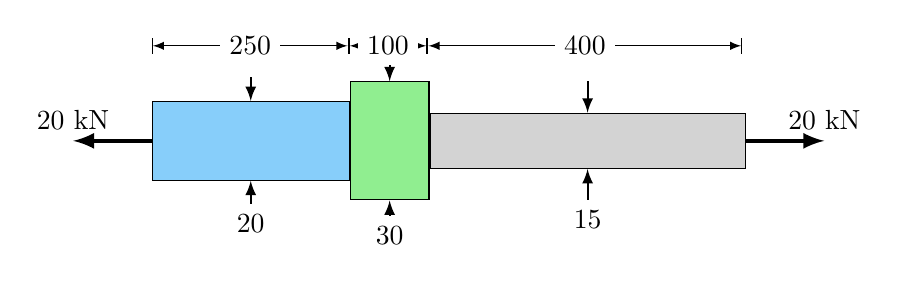
\begin{tikzpicture}
      \node [draw, fill=LightSkyBlue, minimum height=1cm, minimum width=2.5cm](left){};
      \node at (left.east) [anchor=west, draw, fill=LightGreen, minimum height=1.5cm, minimum width=1cm](mid){};
      \node at (mid.east) [anchor=west, draw, fill=LightGrey, minimum height=0.7cm, minimum width=4cm](right){};
      \draw [->, ultra thick] (left.west) --++ (180:1) node[above]{20 kN};
      \draw [->, ultra thick] (right.east) --++ (0:1) node[above]{20 kN};
      \draw [|<->|] (left.north west) ++ (90:0.7) --++ (0:2.5) node[midway, fill=White]{250} node(A){};
      \draw [|<->|] (A.center) --++ (0:1) node[midway, fill=White]{100} node(B){};
      \draw [|<->|] (B.center) --++ (0:4) node[midway, fill=White]{400};
      \draw [<-, thick] (left.north) --++ (90:0.3);
      \draw [<-, thick] (left.south) --++ (-90:0.3) node[below]{20};
      \draw [<-, thick] (mid.north) --++ (90:0.2);
      \draw [<-, thick] (mid.south) --++ (-90:0.2) node[below]{30};
      \draw [<-, thick] (right.north) --++ (90:0.4);
      \draw [<-, thick] (right.south) --++ (-90:0.4) node[below]{15};
    \end{tikzpicture}
  \end{figure} 
  
  \item A 25 mm diameter bar is subjected to an axial tensile load of 100 kN. Under the action of this load a 200 mm gauge length is found to extend 0.19 mm. Determine
  \begin{enumerate}
  \item the modulus of elasticity for the bar material.
  \item the maximum diameter of axial bore (to make the shaft hollow) possible given that the maximum allowable stress is 240 MPa? The load can be assumed to remain constant at 100 kN.
  \item the change in the outside diameter of the bar under the limiting stress quoted in b)? ($E$ = 210 GPa and $v$ = 0.3).
  \end{enumerate} 

  \item The coupling shown below is constructed from steel of rectangular cross-section and is designed to transmit a tensile force of 50 kN. If the bolt is of 15 mm diameter, calculate:
  \begin{enumerate}
  \item the shear stress in the bolt;
  \item the normal stress in the plate;
  \item the normal stress in the forked end of the coupling.
  \end{enumerate}

  \begin{figure}[H]
    \centering
    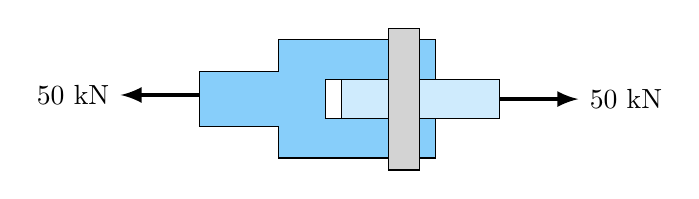
\begin{tikzpicture}
      \draw [fill=LightSkyBlue] (0,0) --++ (0:1) --++ (90:0.4) --++ (0:2) --++ (-90:0.5) --++ (180:1.4) --++ (-90:0.5) --++ (0:1.4) --++ (-90:0.5) --++ (180:2) --++ (90:0.4) --++ (180:1) -- cycle;
      \node at (1.8,-0.1) [anchor=north west, draw, fill=LightSkyBlue!40, minimum height=0.49cm, minimum width=2cm](right){};
      \node at (right.center) [anchor=east, draw, fill=LightGrey, minimum height=1.8cm, minimum width=4mm](){};
      \draw [->, ultra thick] (0,-0.3) --++ (180:1) node[left]{50 kN};
      \draw [->, ultra thick] (right.east) --++ (0:1) node[right]{50 kN};
    \end{tikzpicture}
  \end{figure}

\begin{pycode}
L = random.randint(2,6) # in m
W = L - random.randint(0,L-1) # in m
stress = random.randint(1,10)*1e6 # in Pa
E = random.randint(5,15)*1e10 # in Pa
poisson = random.randint(25,35)/100
\end{pycode}

  \item A thin \py{L} m $\times$ \py{W} m sheet is being stretched along its length by a normal stress of \py{stress/1e6} MPa. The material has $E$ = \py{E/1e9} GPa and $\nu$ = \py{poisson}. Determine the the percentage increase in the area of the sheet.

\begin{pycode}
sigma_allow = random.randint(10,35)*10*1e6 # in Pa
tau_allow = random.randint(5,20)*10*1e6 # in Pa
h = random.randint(4,8)*1e-2 # in m
b = random.randint(2,5)*1e-2 # in m
w = h - 2e-2 # in m
t = random.randint(10,20)/10*1e-2 # 1.0 - 2.0 mm
\end{pycode}

  \item An I-shaped specimen made of a material with $\sigma_{\text{allow}}$ = \py{sigma_allow/1e6} MPa and $\tau_{\text{allow}}$ = \py{tau_allow/1e6} MPa is held with a fixture at each end, determine that maximum tensile load $F$ that can be applied without breaking the specimen. The specimen dimensions are as follows: $w$ = \py{round(w*1e2,1)} cm, $b$ = \py{round(b*1e2,1)} cm, $h$ = \py{round(h*1e2,1)} cm, and the specimen thickness (normal to this page) $t$ = \py{round(t*1e2,1)} cm.
        \begin{figure}[h]
          \centering
          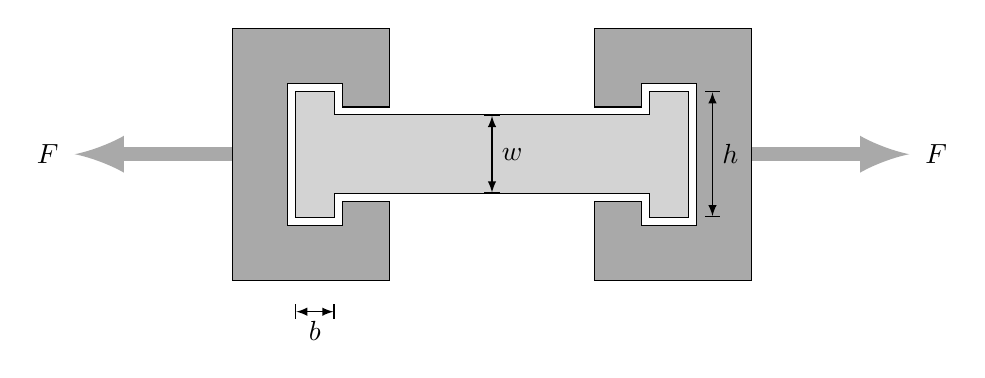
\begin{tikzpicture}[>=latex, rotate=90]
            \draw [fill=LightGrey] (0,0) ++ (0:0.5) --++ (90:2) --++ (0:0.3) --++ (90:0.5) --++ (180:1.6) --++ (-90:0.5) --++ (0:0.3) --++ (-90:4) --++ (180:0.3) --++ (-90:0.5) --++ (0:1.6) --++ (90:0.5) --++ (180:0.3) --++ (90:2);
            \draw [fill=DarkGrey] (0,0) ++ (0:0.5) ++ (90:1.3) ++ (0:0.1) --++ (90:0.6) --++ (0:0.3) --++ (90:0.7) --++ (180:1.8) --++ (-90:0.7) --++ (0:0.3) --++ (-90:0.6) --++ (180:1) --++ (90:2) --++ (0:3.2) --++ (-90:2) -- cycle;
            \begin{scope}[yscale=-1, xscale=1]
              \draw [fill=DarkGrey] (0,0) ++ (0:0.5) ++ (90:1.3) ++ (0:0.1) --++ (90:0.6) --++ (0:0.3) --++ (90:0.7) --++ (180:1.8) --++ (-90:0.7) --++ (0:0.3) --++ (-90:0.6) --++ (180:1) --++ (90:2) --++ (0:3.2) --++ (-90:2) -- cycle;
              \draw [->, line width=5pt, DarkGrey] (0,3.3) --++ (90:2) node[right, Black]{$F$};
            \end{scope}
            \draw [->, line width=5pt, DarkGrey] (0,3.3) --++ (90:2) node[left, Black]{$F$};
            \draw [|<->|] (-2,2) --++ (90:0.5) node[below, midway]{$b$};
            \draw [|<->|] (-0.5,0) --++ (0:1) node[right, midway]{$w$};
            \draw [|<->|] (-0.8,-2.8) --++ (0:1.6) node[right, midway]{$h$};
          \end{tikzpicture}
        \end{figure}

\end{exercises}
%%%%%%%%%%%%%%%%%%%%%%%%%%%%%%%%%%%%%%%%%%%%%%%%%%%%%%%%%%%%%%%%%%%%%%%%%%%%%%%%%%%%%%%%%%%%%%%%%%%%%%%%%%%%%%%%%%%%%%%%%%%%%%%%%%%%%%%%%%%%%%%%%%%%%%%%%%%%%%%%%%%%%%%%%%%%%%

\chapter{Analysis of Axially Loaded Members}
\label{chap: axially loaded members}

Structural components subjected only to tension or compression are known as axially loaded members. We can think of multiple types of such structures, for example, solid bars with straight longitudinal axes which can withstand both compression and tension, or cables, which can only withstand tension. The stress-strain behavior of such members was already discussed in \Cref{chap: basic mechanics of materials}, where we also obtained equations for the stresses acting on cross sections and the strains in longitudinal directions.

In this chapter we consider several other aspects of axially loaded members, beginning with the determination of changes in lengths caused by loads. The calculation for changes in lengths is also important in the analysis of structures whose stresses cannot simply be determined from the loads alone (statically indeterminate structures). We will then also discuss the effect of temperature change to the deformation of axially loaded members.


\section{Statically Determinate Systems}

Structures whose stresses and deformations can be analyzed simply by considering the applied loads are referred to as statically determinate systems. To analyze structures that fall into this category, we have to draw free body diagrams and use the equilibrium equation to determine the internal forces in the cross sections of interest, which would then lead to the stresses in the cross sections. In Chapter 1 we have already discussed the relationship between the internal forces and the stresses and its relationship with strain. We will now discuss the relationship between the deformation of axially loaded members (change in length) and the applied loads.

\subsection{Changes in Length of Axially Loaded Members}

When determining the changes in length of axially loaded members, it is convenient to begin with a coil spring. When a load is applied along the axis of a spring, the spring gets shorter or longer depending on the direction of the load.
Similarly, in the case of axially loaded members, they elongate or shorten depend on the direction of the load. If the load acts toward the member, it is in compression. If the load acts away from the member, it is in tension. It is also important to note its natural length L, also called its free length or relaxed length. Once the member is loaded, supposedly in tension, it will lengthen by an amount $\delta$ and its final length becomes $L + \delta$. If the material of the spring is linearly elastic, the load and elongation will be proportional, following Hooke’s law that

\begin{figure}[h]
  \centering
  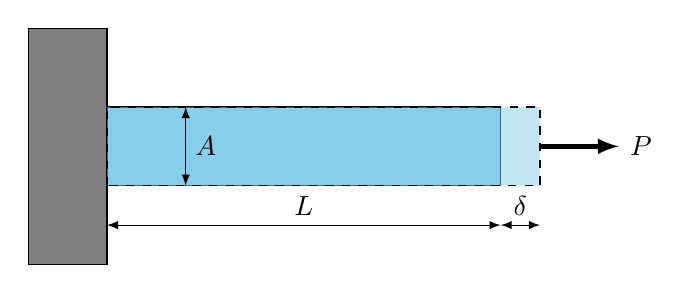
\begin{tikzpicture}
    \draw[fill=Grey] (-1,-1) rectangle (0,2);
    \draw[fill=SkyBlue] (0,0) rectangle (5,1);
    \draw[fill=SkyBlue, fill opacity=0.5, dashed] (0,0) rectangle (5.5,1);
    \draw[->,ultra thick] (5.5,0.5) -- (6.5,0.5) node[right]{$P$};
    \draw[<->] (0,-0.5) -- (2.5,-0.5) node[above]{$L$} -- (5,-0.5);
    \draw[<->] (5,-0.5)-- (5.25,-0.5) node[above]{$\delta$} -- (5.5,-0.5);
    \draw[<->] (1,0) -- (1, 0.5) node[right]{$A$} -- (1,1);
  \end{tikzpicture}
  \caption{Deformation of a axially loaded constant cross-sectioned member.}
\end{figure}

\begin{gather}
 \sigma      = \dfrac{P}{A} \\
 \varepsilon = \dfrac{\delta}{L} \\
 \sigma      = E\varepsilon 
\end{gather}

And therefore we can derive for these relationships that

\begin{equation}
  \delta  = \frac{PL}{AE}
\end{equation}

This equation shows that the elongation is directly proportional to the load $P$ and the member length $L$, and inversely proportional to the modulus of elasticity $E$ and the cross-sectional area $A$. This equation works assuming that the bar has a uniform cross section.

\subsection{Change in Length of Nonuniform Members}

However, if the bar is loaded by different axial loads, bar made of different materials, or its cross sectional area varies throughout its length, the stress throughout the bar varies. To solve for the total change in length of this type of problem, we must 1) identify the segments of the bar, 2) determine the axial forces in the segments from the free body diagrams, 3) applies the equation to all segments. The total change in length is the sum of the changes in length in all segments, or

\begin{figure}[h]
  \centering
  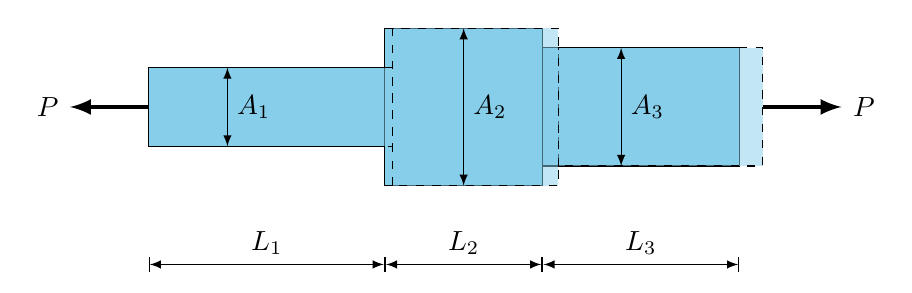
\begin{tikzpicture}
    %members
    \draw[fill=SkyBlue] (0,0) rectangle (3,1) ;
    \draw[fill=SkyBlue] (3,-0.5) rectangle (5,1.5);
    \draw[fill=SkyBlue] (5,-0.25) rectangle (7.5,1.25);
    % extended members
    \draw[fill=SkyBlue, fill opacity=0.5, dashed] (0,0) rectangle (3.1,1) ;
    \draw[fill=SkyBlue, fill opacity=0.5, dashed] (3.1,-0.5) rectangle (5.2,1.5);
    \draw[fill=SkyBlue, fill opacity=0.5, dashed] (5.2,-0.25) rectangle (7.8,1.25);
    %force
    \draw[->,ultra thick] (7.8,0.5) -- (8.8,0.5) node[right]{$P$};
    \draw[<-,ultra thick] (-1,0.5) node[left]{$P$} -- (0,0.5);
    %lengths
    \draw[|<->|] (0,-1.5) -- (1.5,-1.5) node[above]{$L_1$} -- (3,-1.5);
    \draw[|<->|] (3,-1.5)-- (4,-1.5) node[above]{$L_2$} -- (5,-1.5);
    \draw[|<->|] (5,-1.5)-- (6.25,-1.5) node[above]{$L_3$} -- (7.5,-1.5);
  %areas
    \draw[<->] (1,0) -- (1, 0.5) node[right]{$A_1$} -- (1,1);
    \draw[<->] (4,-0.5) -- (4, 0.5) node[right]{$A_2$} -- (4,1.5);
    \draw[<->] (6,-0.25) -- (6, 0.5) node[right]{$A_3$} -- (6,1.25);
  \end{tikzpicture}
\end{figure}

\begin{equation}
  \delta  = \sum\limits_{i = 1}^n \frac{{P_i}{L_i}}{{E_i}{A_i}}
\end{equation}

In which $i$ is the index of various segments of the bar and $n$ is the total number of segments. Note that the force $P_i$ is the internal axial force in the segment $i$, not the external force.

Some other times, the axial force $P$ and the cross-sectional area $A$ vary continuously along the axis of a bar. In this case, instead of using an algebraic sum, we must integrate the small changes along the length of a bar to calculate the total change in length.

Consider a small slither of the bar that has length $dx$ and cross-sectional area $A(x)$ locating at a distance $x$ from one end of the bar. Assume the internal force acting on the slither of the bar follows the function $P(x)$. The change in length of the slither is simply

\begin{figure}[h]
  \centering
  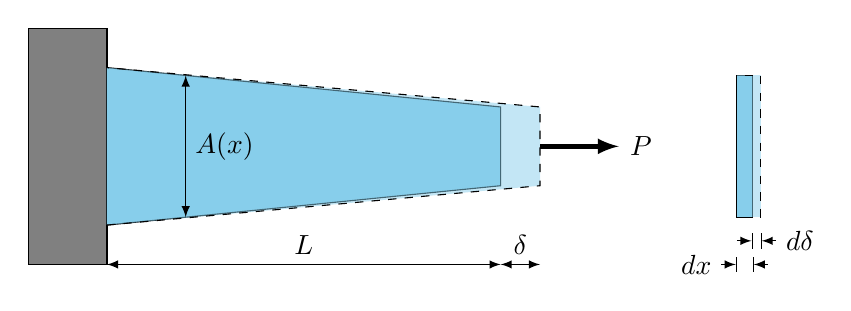
\begin{tikzpicture}
    \draw[fill=Grey] (-1,-1) rectangle (0,2);
    \draw[fill=SkyBlue] (0,-0.5) -- (5,0) -- (5,1) -- (0,1.5);
    \draw[fill=SkyBlue, fill opacity=0.5, dashed] (0,-0.5) -- (5.5,0) -- (5.5,1) -- (0,1.5);
    \draw[->,ultra thick] (5.5,0.5) -- (6.5,0.5) node[right]{$P$};
    \draw[<->] (0,-1) -- (2.5,-1) node[above]{$L$} -- (5,-1);
    \draw[<->] (5,-1)-- (5.25,-1) node[above]{$\delta$} -- (5.5,-1);
    \draw[<->] (1,-0.4) -- (1, 0.5) node[right]{$A(x)$} -- (1,1.4);

    \draw[fill=SkyBlue] (8,-0.4) rectangle (8.2,1.4);
    \draw[fill=SkyBlue, fill opacity=0.5, dashed] (8,-0.4) rectangle (8.3,1.4);
    \draw[->|] (7.8,-1) node[left]{$dx$}  to (8,-1);
    \draw[|<-] (8.2,-1) to (8.4,-1);
    \draw[->|] (8,-0.7) to (8.2,-0.7);
    \draw[|<-] (8.3,-0.7) to (8.5,-0.7) node[right]{$d\delta$};
  \end{tikzpicture}
  \caption{Deformation of a axially loaded constant cross-sectioned member.}
\end{figure}

  \[d\delta  = \frac{{P(x)dx}}{{EA(x)}}\]

And the total elongation of the entire bar is

\begin{equation}
  \delta  = \int_0^L {d\delta }  = \int_0^L {\frac{{P(x)dx}}{{EA(x)}}}
\end{equation}

\begin{example}
  A cylinder with continuously variable cross sections of length $L$ is supported at end A and subjected to a tensile load $P$ at the free end B. The radii of the bar at ends A and B are $r_A$ and $r_B$ respectively. Determine the elongation of the bar due to the load $P$.
  \begin{figure}[H]
    \centering
    % 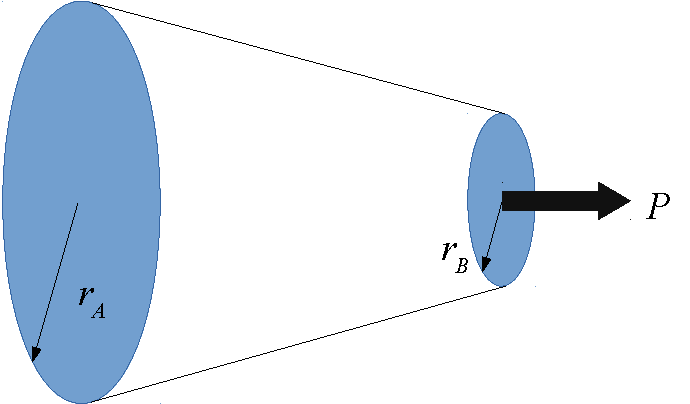
\includegraphics[scale=0.6]{pictures/Axial-load/axial-load-cone}
    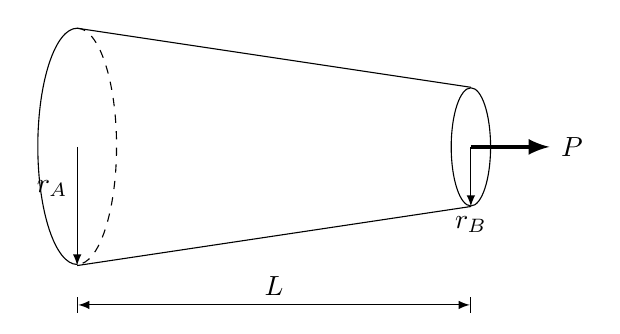
\begin{tikzpicture}
      \node [ellipse, dashed, minimum height=3cm, minimum width=1cm](left){};
      \draw (left.north) arc (90:270:0.5 and 1.5);
      \draw [dashed] (left.north) arc (90:-90:0.5 and 1.5);
      \node [ellipse, xshift=5cm, minimum height=1.5cm, minimum width=0.5cm, draw](right){};
      \draw
      (left.north) -- (right.north)
      (left.south) -- (right.south);
      \draw [->] (left.center) -- (left.south) node[midway, above left]{$r_A$};
      \draw [->] (right.center) -- (right.south) node[below]{$r_B$};
      \draw [->, ultra thick] (right.center) --++ (0:1) node[right]{$P$};
    \draw [|<->|] (left.south) ++ (-90:0.5) --++ (0:5) node[midway, above]{$L$};
    \end{tikzpicture}
  \end{figure}
\end{example}

\begin{solution}
  From the equation
  
\[\delta  = \int_0^L d\delta  = \int_0^L \frac{P(x)dx}{EA(x)} \]

We know that the load is constant throughout the length of the cylinder. The only thing varying is the diameter of the cross section. Therefore, we will write the diameter as a function of length.
First to simplify the expression for the integral, we set the origin of the $x$ coordinate by extending the sides of the tapered bar until they meet at point O.
The distance $L_A$ and $L_B$ from the origin O to ends A and B respectively are in the ratio

\begin{figure}[H]
  \centering
  % 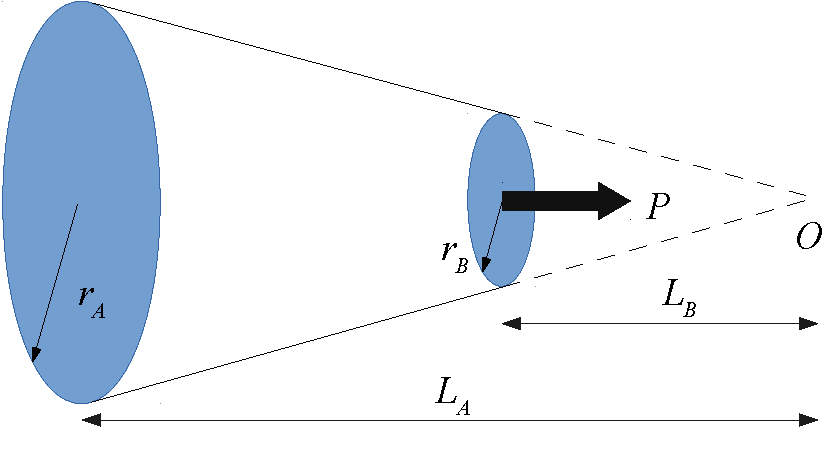
\includegraphics[scale=0.6]{pictures/Axial-load/axial-load-cone-mod}
  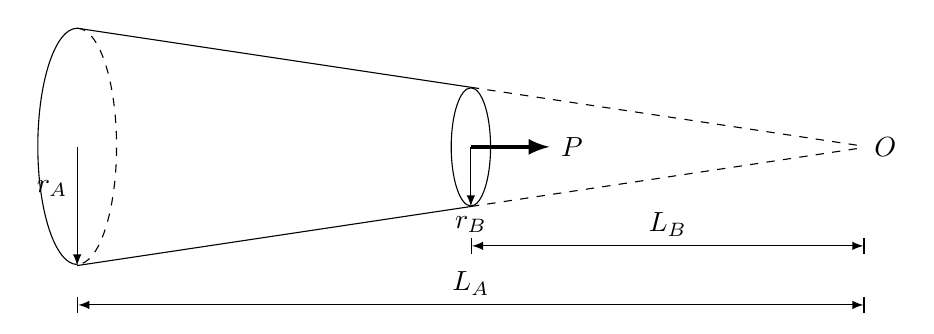
\begin{tikzpicture}
    \node [ellipse, dashed, minimum height=3cm, minimum width=1cm](left){};
    \draw (left.north) arc (90:270:0.5 and 1.5);
    \draw [dashed] (left.north) arc (90:-90:0.5 and 1.5);
    \node [ellipse, xshift=5cm, minimum height=1.5cm, minimum width=0.5cm, draw](right){};
    \draw
    (left.north) -- (right.north)
    (left.south) -- (right.south);
    \draw [dashed]
    (right.north) --++ (5,-0.75)
    (right.south) --++ (5,0.75) node(O){} node[right]{$O$};
    \draw [->] (left.center) -- (left.south) node[midway, above left]{$r_A$};
    \draw [->] (right.center) -- (right.south) node[below]{$r_B$};
    \draw [->, ultra thick] (right.center) --++ (0:1) node[right]{$P$};
    \draw [|<->|] (left.south) ++ (-90:0.5) --++ (0:10) node[midway, above]{$L_A$};
    \draw [|<->|] (right.south) ++ (-90:0.5) --++ (0:5) node[midway, above]{$L_B$};
  \end{tikzpicture}
\end{figure}

\[\frac{L_A}{L_B} = \frac{r_A}{r_B}\]	

Using similar triangles, we have that the radius $r(x)$ at the distance $x$ from the origin to the radius $r_A$ at the small end of the bar is

\[\frac{r(x)}{r_A} = \frac{x}{L_A} \text{  or  } r(x) = \frac{r_Ax}{L}\]	

Therefore, the cross-sectional area at distance $x$ from the origin is

\[A(x) = \pi [r(x)]^2 = \frac{\pi r_A^2x^2}{L_A^2}\]

The change in length is, thus,

\[\delta  = \int_{L_A}^{L_B} \frac{Pdx(L_A^2)}{E\pi r_A^2x^2} \]

Performing the integration, we have

\[\delta  = \frac{PL_A^2}{E\pi r_A^2}\left[ - \frac{1}{x} \right]_{L_A}^{L_B} = \frac{PL_A^2}{E\pi r_A^2}\left( \frac{1}{L_A} - \frac{1}{L_B} \right)\]	

The quantity in the parentheses can be simplified to

\[\left( \frac{1}{L_A} - \frac{1}{L_B} \right) = \frac{L_B - L_A}{L_AL_B} = \frac{L}{L_AL_B}\]	

So the equation becomes

\[\delta  = \frac{PL_A^2}{E\pi r_A^2}\frac{L}{L_AL_B} = \frac{PL}{E\pi r_A^2}\left( \frac{L_A}{L_B} \right)\]	

Finally, we know from similar triangles that $L_A/L_B = r_A/r_B$.

\[\delta  = \frac{PL}{E\pi r_A^2}\left( \frac{r_A}{r_B} \right) = \frac{PL}{\pi Er_Ar_B}\]

\end{solution}

\section{Statically Indeterminate Systems}

In the case where the deformation of the member can be determine solely from equation of equilibrium and free-body diagram, the structure of that type is classified as statically determinate. It is also important to note that the force in this type of structure can be determined without the knowledge of properties of the materials.

However, most structures are more complex than this. The internal forces and reactions cannot be determined from the equation of equilibrium alone. For example, consider a bar that is attached on both sides to walls. A force P is applied in the middle of the beam towards the right wall. Now, it is impossible to determine the internal force and reaction forces since there is only one useful equation of equilibrium but two unknown forces (reaction forces at either end). This type of structure is classified as statically indeterminate. To analyze such structures we must supplement the equilibrium equations with additional equations pertaining to the displacement of the structure.

The equation that pertains to the displacement requirements of the structure is called an equation of \emph{compatibility} or \emph{kinematic} equation.

To solve both the equation of equilibrium and equation of compatibility, we must establish the relationship between the force and displacement, this we can borrow from our knowledge of statically determinate system of axially loaded members that
	
We shall now look at a simple example to better understand the steps in analyzing statically indeterminate system.

\begin{example}
  A circular bar AB is fixed on both end between the two walls of the same distance apart as the unstretched length of the bar $L$. The bar has a constant cross-sectional area $A$. Force $P$ is exerted on the bar at point C. Find the reaction at both point A and B.
  \centering
  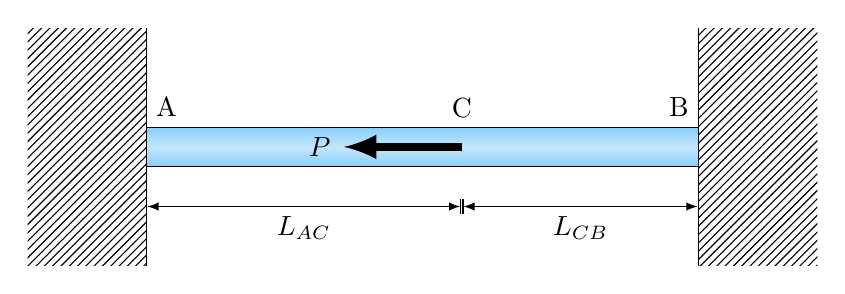
\begin{tikzpicture}
    \node [rectangle, pattern=north east lines, minimum height=3cm, minimum width=1.5cm](lwall){};
    \draw (lwall.south east) -- (lwall.north east);
    \node at (lwall.east) [anchor=west, draw, rectangle, top color=LightSkyBlue, bottom color=LightSkyBlue, middle color=LightSkyBlue!50, minimum height=5mm, minimum width=7cm](bar){};
    \node at (bar.east) [anchor=west, rectangle, pattern=north east lines, minimum height=3cm, minimum width=1.5cm](rwall){};
    \draw (rwall.south west) -- (rwall.north west);
    \node at (bar.north west) [above right]{A};
    \node at (bar.north east) [above left]{B};
    \draw [->, line width=3pt] (bar.center) ++ (0:0.5) node[above, yshift=0.2cm]{C} --++ (180:1.5) node[left]{$P$};
    \draw [|<->|] (bar.south west) ++ (-90:0.5) --++ (0:4) node[midway, below]{$L_{AC}$};
    \draw [|<->|] (bar.south east) ++ (-90:0.5) --++ (180:3) node[midway, below]{$L_{CB}$};
  \end{tikzpicture}
\end{example}
\begin{solution}
First, we know that there would be reactions at both points A and B. Using the equation of equilibrium, we know that the bar is in equilibrium, and therefore

\[\sum F  = 0 = P - {F_A} - {F_B}\]

We also know that the bar is restrained between two walls, preventing any length change so that the deformation of segment AC and CB must sum up to zero.

\[{\delta _{AC}} + {\delta _{CB}} = 0\]

Finally, we apply force-displacement relationship based on Hooke’s law. We know that the force in segment AC is $F_A$ in the compressive direction, and that the force in segment CB is $F_B$ in the tensile direction. We substitute the force-displacement relationship into the compatibility equation so that we have

\[ - \frac{{{F_A}{L_{AC}}}}{{AE}} + \frac{{{F_B}{L_{CB}}}}{{AE}} = 0\]	

Solving this equation, we have

\[{F_B} = \frac{{{L_{AC}}}}{{{L_{CB}}}}{F_A}\]	

So the magnitude of the reaction is inversely proportional to the distance away from the applied load. Substitute the solution into the equation of equilibrium, we have

\[\begin{gathered}
  {F_A} = \frac{{{L_{CB}}}}{L}P \hfill \\
  {F_B} = \frac{{{L_{AC}}}}{L}P \hfill \\ 
\end{gathered} \]
\end{solution}

\begin{example} Three bars attached to a rigid beam
  \begin{figure}[H]
    \centering
    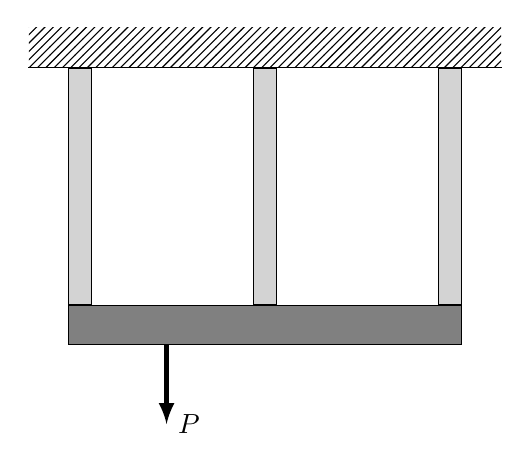
\begin{tikzpicture}[>=latex]
      \node [draw, rectangle, minimum height=0.5cm, minimum width=5cm, fill=Grey](rigid){};
      \node at (rigid.north west) [anchor=south west, draw, fill=LightGrey, minimum height=3cm, minimum width=3mm](left){};
      \node at (rigid.north) [anchor=south, draw, fill=LightGrey, minimum height=3cm, minimum width=3mm](mid){};
      \node at (rigid.north east) [anchor=south east, draw, fill=LightGrey, minimum height=3cm, minimum width=3mm](right){};
      \node at (mid.north) [anchor=south, minimum height=5mm, minimum width=6cm, pattern=north east lines](ceil){};
      \draw (ceil.south west) -- (ceil.south east);
      \draw [->, ultra thick] (rigid.south) ++ (180:1.25) --++ (-90:1) node[right]{$P$};
    \end{tikzpicture}
  \end{figure}

  Determine the internal forces in the three vertical members if they have the same $A$ and $E$?
\end{example}
\begin{solution}

  Drawing a free body diagram of each component shows that the application of equlibrium equation should be done on the rigid beam to express $P$ in terms of internal forces in the members $F_1, F_2, F_3$. Assuming all internal forces are tensile, they all point upward on the rigid beam. As such, the force equilibrium equation can be written as.

 \[ F_1 + F_2 + F_3 = P \]

 The internal forces and not acting along the axis of the rigid beam, hence we must make sure that the total moment on the beam is zero as well. Using the leftmost point on the rigid beam as a fulcrum, we have that

 $$ F_2 L + F_3 (2L) = P \frac{L}{2} $$

 This can be reduced to 

 $$ F_2 + 2F_3 = \frac{P}{2} $$

 At this point we have 3 unknown internal forces, but only 2 equations. We need an additional one using compatibility equation

 At this point we have 3 unknown internal forces, but only 2 equations. We need an additional one using compatibility equation. In this problem, the horizontal rigid beam is key. Being rigid, the beam must remain straight (though not necessarily horizontal), and we can use this to derive our compatibility equation. The problem is asymmetrical, as $P$ is off-center, so we may assume that the rigid beam would tilt slightly. This will results in the deformation of all three members being proportional, as shown in the following figure.

 % \begin{figure}[H]
 % \end{figure}

 From the given geometry, we can derive a compatibility equation using a similar triangle relation.

 $$ \frac{\delta_1 - \delta_3}{2L} = \frac{\delta_2 - \delta_3}{L} $$
 $$ \delta_1 - \delta_3 = 2\delta_2 - 2\delta_3 $$
 $$ \delta_1 = 2\delta_2 - \delta_3 $$

 The next step is to convert the compatibility equation to its expression in force using Hooke's law.

 $$ \frac{F_1 L}{AE} = 2\frac{F_2 L}{AE} - \frac{F_3 L}{AE} $$
 $$ F_1 = 2F_2 - F_3 $$

 We now have the third equation to solve for our system. You may choose to solve for each internal force in any order, though in this example we will start with $F_3$. So write all other internal forces in terms of $F_3$.

 $$ F_2 = \frac{P}{2} - 2F_3 $$
 $$ F_1 = 2F_2 - F_3 = P - 5F_3 $$

 Now, substitute this into the first equilibrium equation.

 $$ F_1 + F_2 + F_3 = P - 5F_3 + \frac{P}{2} - 2F_3 + F_3 = P $$
 $$ 6F_3 = \frac{P}{2} $$
 $$ F_3 = \frac{P}{12} $$

 $$ F_1 = P - 5 \frac{P}{12} = \frac{7P}{12} $$
 $$ F_2 = \frac{P}{2} - \frac{2P}{12} = \frac{P}{3} $$
\end{solution}


\section{Statically Indeterminate Systems with Thermal Effects}

As mentioned in section 1.3, external loads are not the only sources of stress and strains in a structure. Changes in temperature can produce expansion or contraction of the material, resulting in thermal strains and stresses.

In statically indeterminate structures, the total change in length when considering thermal effects is simply the sum of the change from external loads and the change from thermal effects. Similarly, in the case of statically indeterminate structures, thermal effects apply directly into equations of compatibility. After the effect has been properly accounted for, the structures can be analyzed as normal.

\begin{example}
  Using the previous example of the bar fixed at both ends between the walls. Once the force $P$ is applied, what is the change in temperature so that there is no stress in segment AC? Assume that the material of the bar has Young’s modulus $E$ and cross-sectional area $A$.
  
  \centering
  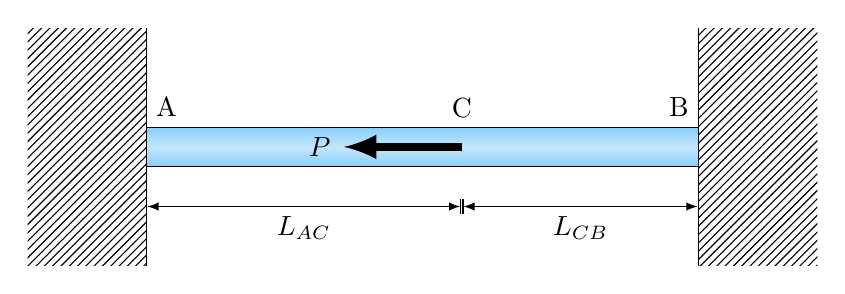
\begin{tikzpicture}
    \node [rectangle, pattern=north east lines, minimum height=3cm, minimum width=1.5cm](lwall){};
    \draw (lwall.south east) -- (lwall.north east);
    \node at (lwall.east) [anchor=west, draw, rectangle, top color=LightSkyBlue, bottom color=LightSkyBlue, middle color=LightSkyBlue!50, minimum height=5mm, minimum width=7cm](bar){};
    \node at (bar.east) [anchor=west, rectangle, pattern=north east lines, minimum height=3cm, minimum width=1.5cm](rwall){};
    \draw (rwall.south west) -- (rwall.north west);
    \node at (bar.north west) [above right]{A};
    \node at (bar.north east) [above left]{B};
    \draw [->, line width=3pt] (bar.center) ++ (0:0.5) node[above, yshift=0.2cm]{C} --++ (180:1.5) node[left]{$P$};
    \draw [|<->|] (bar.south west) ++ (-90:0.5) --++ (0:4) node[midway, below]{$L_{AC}$};
    \draw [|<->|] (bar.south east) ++ (-90:0.5) --++ (180:3) node[midway, below]{$L_{CB}$};
  \end{tikzpicture}
\end{example}
\begin{solution}

  There are still support forces at A and B. The equilibrium equation in this case would remain the same

  \[\sum F  = 0 = P - {F_A} - {F_B}\]

  Also, as the bar is still fixed at both ends, it cannot change in length. Therefore the sum of the change in length of both segments must be zero.

  \[{\delta _{AC}} + {\delta _{CB}} = 0\]	

  Finally, we apply force-displacement relationship based on Hooke’s law. We know that the force in segment AC is $F_A$ in the compressive direction, and that the force in segment CB is $F_B$ in the tensile direction. However, there is also the change in length of each segment due to the temperature change, so we must substitute in the change in length of both segments with force-displacement and displacement-temperature change relationships
  
  \[\begin{gathered}
      - \frac{F_AL_{AC}}{AE} + \alpha \Delta T{L_{AC}} + \frac{F_BL_{CB}}{AE} + \alpha \Delta T{L_{CB}} = 0 \\ 
      - \frac{F_AL_{AC}}{AE} + \frac{F_BL_{CB}}{AE} + \alpha \Delta T(L_{CB} + L_{AC}) = 0 \\ 
      - \frac{F_AL_{AC}}{AE} + \frac{F_BL_{CB}}{AE} + \alpha \Delta TL = 0 \\ 
    \end{gathered} \]	
  
  Solving this equation we have
  
  \[\begin{gathered}
      {F_A} = P\frac{L_{CB}}{L} + \frac{\alpha \Delta T}{AE} \hfill \\
      {F_B} = P\frac{L_{AC}}{L} - \frac{\alpha \Delta T}{AE} \hfill \\ 
    \end{gathered} \]
  
  To reduce the stress in segment AC to zero, its internal force must be zero, and therefore the reaction at A must be zero. Setting $F_A = 0$, we have
  
  \[\Delta T =  - \frac{{PAE}}{\alpha }\frac{{{L_{CB}}}}{L}\]
  
\end{solution}

\begin{example} Three bars and a rigid beam under thermal change

  The leftmost and rightmost members have identical thermal properties $\alpha_1$, while the middle member has $\alpha_2$.

  \centering
  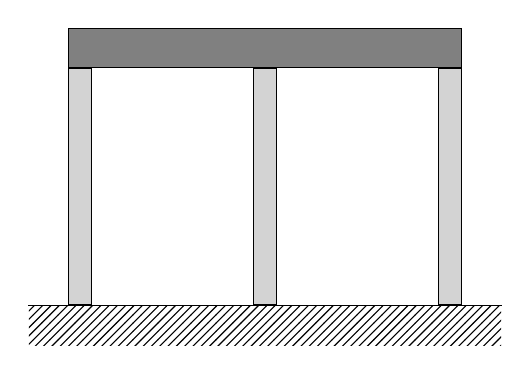
\begin{tikzpicture}[>=latex]
    \node [draw, rectangle, minimum height=0.5cm, minimum width=5cm, fill=Grey](rigid){};
    \node at (rigid.south west) [anchor=north west, draw, fill=LightGrey, minimum height=3cm, minimum width=3mm](left){};
    \node at (rigid.south) [anchor=north, draw, fill=LightGrey, minimum height=3cm, minimum width=3mm](mid){};
    \node at (rigid.south east) [anchor=north east, draw, fill=LightGrey, minimum height=3cm, minimum width=3mm](right){};
    \node at (mid.south) [anchor=north, minimum height=5mm, minimum width=6cm, pattern=north east lines](ceil){};
    \draw (ceil.north west) -- (ceil.north east);
  \end{tikzpicture}

  If the temperatures of the vertical bars are increased by $\Delta T$, determine the internal force in each member.
\end{example}
\begin{solution}
  First we must establish equilibrium equations for the members. For the force equilibrium in $y$-axis, we have

  $$ F_1 + F_2 + F_3 = 0 $$

  A second equilibrium equation can be derived in one of the two ways. The first exploits the problem's symmetry about the middle member.

  $$ F_1 = F_3 $$

  Substituting this into the force equilibrium equation gives

  $$ F_2 = 2F_3 = 2F_1 $$
  
  The second method employs the moment equilibrium about the left side of the rigid beam.

  $$ F_2 L + F_3 (2L) = 0 $$
  $$ F_2 = -2F_3 $$

  Moment equilibrium about the right side of the rigid beam gives the same equation.

  $$ F_2 = -2F_1 = 2F_3 $$

  The next step is to determine the compatibility equation. We can still apply similar triangle equation, but it is obvious that, with symmetry, all three vertical members undergo identical deformations. 

  $$ \delta_1 = \delta_2 = \delta_3 $$

  Converting deformation to internal force and thermal change, we have

  $$ \frac{F_1 L}{AE} + \alpha_1 \Delta TL = \frac{F_2 L}{AE} + \alpha_2 \Delta TL $$ 

  Substituting $F_1 = F_2 / 2$, we have

  $$ F_2 = \frac{2}{3} \left( \alpha_1 - \alpha_2 \right) \Delta T A E $$
  $$ F_1 = F_3 = \frac{1}{3} \left( \alpha_2 - \alpha_1 \right) \Delta T A E $$

  Now, let us analyze the solution. We have previously assumed all internal forces tensile, so if the sign comes out positive, the force \emph{is} tensile. It is compressive otherwise. For $\alpha_1 > \alpha_2$ and $\Delta T > 0$

  $$ F_2 > 0 \text{ and } F_1, F_3 < 0 $$

  When the members are heated the left and right members will try to expand more than the middle one due to their higher coefficients of thermal expansion $\alpha_1$. However, because of the rigid beam restriction, the left and right members are squeezed down, while the middle part is pulled. Other situations can be analyzed with similar logic.
\end{solution}

\section{Compound Bars}

Increasing uses of composite materials dictates the need for us to understand their mechanical behavior. For an axially loaded component made of composite materials, the simplest of these are compound bars. A compound bar is defined by an axially loaded member whose various materials that make up its cross section undergo the exact elongation/contraction as all the other materials.

\begin{figure}[h]
  \centering
  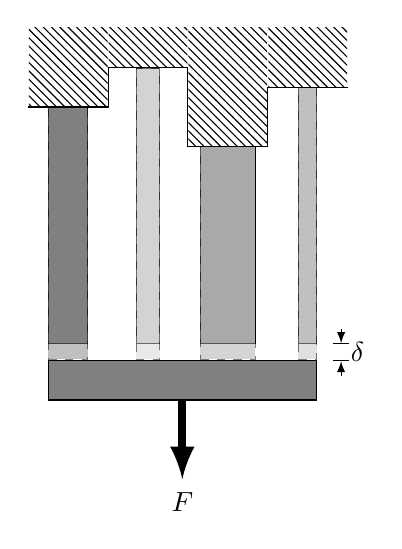
\begin{tikzpicture}[>=latex]
    \node [minimum height=1cm, pattern=north west lines, minimum width=1cm](wall1){};
    \node at (wall1.north east)[anchor=north west, minimum height=0.5cm, pattern=north west lines, minimum width=1cm](wall2){};
    \node at (wall2.north east)[anchor=north west, minimum height=1.5cm, pattern=north west lines, minimum width=1cm](wall3){};
    \node at (wall3.north east)[anchor=north west, minimum height=0.75cm, pattern=north west lines, minimum width=1cm](wall4){};

    \draw (wall1.south west) -- (wall1.south east) -- (wall2.south west) -- (wall2.south east) -- (wall3.south west) -- (wall3.south east) -- (wall4.south west) -- (wall4.south east);

    \node at (wall1.south) [anchor=north, draw, minimum height=3cm, minimum width=5mm, fill=Grey](bar1){};
    \node at (wall2.south) [anchor=north, draw, minimum height=3.5cm, minimum width=3mm, fill=LightGrey](bar2){};
    \node at (wall3.south) [anchor=north, draw, minimum height=2.5cm, minimum width=7mm, fill=DarkGrey](bar3){};
    \node at (wall4.south) [anchor=north, draw, minimum height=3.25cm, minimum width=2mm, fill=Silver](bar4){};
    
    \node at (wall1.south) [anchor=north, dashed, draw, minimum height=3.2cm, minimum width=5mm, fill=Grey, opacity=0.5](bar1e){};
    \node at (wall2.south) [anchor=north, dashed, draw, minimum height=3.7cm, minimum width=3mm, fill=LightGrey, opacity=0.5](bar2e){};
    \node at (wall3.south) [anchor=north, dashed, draw, minimum height=2.7cm, minimum width=7mm, fill=DarkGrey, opacity=0.5](bar3e){};
    \node at (wall4.south) [anchor=north, dashed, draw, minimum height=3.45cm, minimum width=2mm, fill=Silver, opacity=0.5](bar4e){};

    \node at (bar1e.south west) [anchor=north west, draw, minimum height=5mm, minimum width=3.4cm, fill=Grey](bar){};

    \draw [line width=3pt, ->] (bar.south) --++ (-90:1) node[below]{$F$};
    \draw [|<-] (bar4.south east) ++ (0:0.3) --++ (90:0.2) node[at start, right, yshift=-1mm]{$\delta$};
    \draw [|<-] (bar4e.south east) ++ (0:0.3) --++ (-90:0.2);
  \end{tikzpicture}
  \caption{An axially loaded compound bar}
  \label{fig: compound bar}
\end{figure}

\subsection{Internal Force}

The governing equation of deformation in member $i$ of the compound bar can be expressed as

\begin{align*}
  \delta_i = \frac{F_i L_i}{A_i E_i}
\end{align*}

By definition, all members in a compound bar share identical deformation

\begin{align*}
  \delta_1 = \delta_2 = \ldots = \delta
\end{align*}

Also, due to equilibrium on the horizontal bar, sum of the internal forces must be equal to $F$, which allows us to write that

\begin{align}
  \label{eq: compound bar}
  F = \sum F_i &= \sum \frac{\delta A_i E_i}{L_i} \nonumber \\
  \frac{F_i}{F} &= \frac{\dfrac{A_iE_i}{L_i}}{\sum \dfrac{A_iE_i}{L_i}}
\end{align}

\subsection{Compound Modulus}

To evaluate the modulus of the compound bar as a single material, the members must have identical lengths (the reason for which will be discussed soon). We can derive the relationship of the modulus of the compound bar, aka \emph{compound modulus}, as follows.

\begin{align*}
  F &= F_1 + F_2 + \ldots + F_n \\
  \sigma A &= \sigma_1 A_1 + \sigma_2 A_2 + \ldots + \sigma_n A_n 
\end{align*}

At this point, we are going to divide through both sides by a commond strain $\epsilon$. We can do this because members of a compound bar share the same elongations/contractions and, as we introduced earlier in this section, they now share the same lengths. Therefore, when the members have the same length and the same elongations/contractions, they definitely have the same strains. Now, we can proceeed.

\begin{align}
  \label{eq: compound modulus}
  \frac{\sigma}{\epsilon} A &= \frac{\sigma_1}{\epsilon} A_1 + \frac{\sigma_2}{\epsilon} A_2 + \ldots + \frac{\sigma_n}{\epsilon} A_n \nonumber \\
  E_cA &= E_1 A_1 + E_2A_2 + \ldots + E_nA_n \nonumber \\
  E_c &= \dfrac{\sum E_iA_i}{\sum A_i}
\end{align}

It is worth noting in the end that the compound modulus is simply the area-weighted average of the moduli of the members.

\section{** Inelastic Deformation **}

In the previous sections, we have discussed the analysis of structures when the material stress never exceeds yield strength. However, in some engineering applications, especially in designing steel members, the design must take into account the behavior after the stress has reached yield strength. To meaningfully analyze the behavior into the plastic regime of deformation, we must first introduce the concept of elastic perfectly plastic materials.

\subsection{Elastic perfectly plastic materials}

In this type of material, the stress-strain behavior is linear throughout its elastic region. However, once the stress reaches yield strength, the material can no longer support additional stress. The strain, on the other hand, will keep increasing even after the stress reaches yield point, resulting in a flat stress-strain diagram after yield point.

\begin{figure}[h]
  \centering
  \begin{tikzpicture}[scale=0.7, >=latex]
    \draw[<->](-5,0)--(5,0) node[right]{$\varepsilon$};
    \draw[<->](0,-5)--(0,-4) node[right]{$-S_y$} -- (0,4) node[left]{$S_y$} -- (0,5) node[right]{$\sigma$};
    \draw[very thick, Blue](-5,-4) -- (-2,-4) -- (2,4) -- (5,4);
  \end{tikzpicture}
  %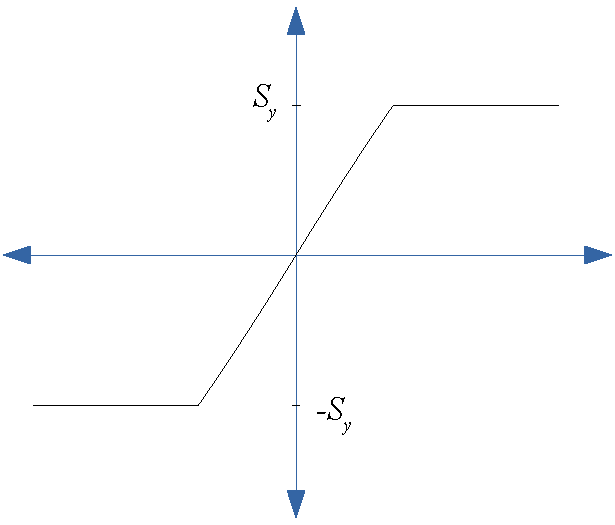
\includegraphics[scale=0.7]{pictures/Axial-load/elastic-perfectly-plastic}
  \caption{Typical behavior of an elastic-perfectly plastic material.}
\end{figure}

\subsection{Residual Stress}

When a material is loaded beyond its yield point, the material will go into plastic deformation for which even after the load is removed, the deformation will remain. When the material is not restrained by supports, the deformation will manifest itself in dimension changes. On the other hand, if the material is restrained, the plastic deformation cannot manifest itself in the form of dimension changes but in residual stress instead. In this case, the methods of solving statically indeterminate problems apply here as well.

We must, however, be mindful that now the material stress-strain response is more complicated—the material is now assumed to be elastic-perfectly plastic. Therefore, after the initial stress analysis through the use of equations of equilibrium and equations of compatibility, we must validate that the stress in any member remains at or below yield point.

To solve a residual stress problem, where there is a cycle of loading and unloading, we must employ the principle of superposition of positive load (loading) and negative load (unloading). The loading results in both elastic and plastic deformations while the unloading results only in an elastic stress. After superposition, the loads will cancel; however, the stress distribution will not cancel and therefore residual stress will remain.

\begin{example}

  A circular bar AB having radius of 1 in is fixed between two walls 5 ft apart. A load $P$ is applied to a point 2 ft from the left wall towards the left wall. The circular bar has a stress-strain response as shown. Find
  \begin{enumerate}
  \item The minimum magnitude of $P$ so that both segments of the beam will start to yield.
  \item The permanent deformation of point C after the force $P$ is removed.
  \end{enumerate}

\end{example}

\begin{solution}
  
  First we find the Young’s modulus of the bar material
  
  \[E = \frac{{(20 \times {{10}^3})}}{{0.001}} = 2 \times {10^7} \text{ psi}\]	
  
  For both segments of the beam to yield, the stresses in both segments must reach yield point, which is at 20 ksi. However, when force $P$ is applied, the left segment will be in compression, while the right will be in tension. Therefore, we have
  
  \begin{align*}
    &{\sigma _{AC}} =  - 20 \times {10^3} \text{ psi} \\
    &{\sigma _{CB}} = 20 \times {10^3} \text{ psi}
  \end{align*}	

  Using equilibrium equation, we can solve for force $P$ from the support forces at A and B.
  
  \begin{align*}
    P = {F_A} + {F_B} &= 2(20 \times {10^3} \text{ psi})(\pi ){(1 \text{ in})^2} \\ 
                      &= 1.26 \times {10^5} \text{ lb}
  \end{align*}	
  
  Note that the support forces at A and B are equal because the stresses in both segments have the same magnitude.
  
  To find the permanent deformation, we first need to find the residual stress. By applying the principle of superposition, we can find the residual stress after unloading by summing the stresses from loading $P$ to the left and to the right. Since we have already found the stresses from loading P to the left, we will proceed to find the stresses from the ‘unloading’ force $P$ at point C to the right.
  
  \begin{align*}
    (\sigma _{AC})_{unload} &= \frac{L_{CB}}{L}\frac{P}{A} = \frac{3}{5} \frac{(1.26 \times 10^5 \text{ lb})}{\pi {(1 \text{ in})^2}} = 2.4 \times {10^4} \text{ psi} \text{ (tensile)} \\
  (\sigma _{CB})_{unload} &= \frac{L_{AC}}{L}\frac{P}{A} = \frac{2}{5} \frac{(1.26 \times 10^5 \text{ lb})}{\pi (1 \text{ in})^2} = 1.6 \times {10^4} \text{ psi} \text{ (compressive)}
  \end{align*}	
  
  Note that we do not need to be concern about the stress going beyond the yield point in the unloading case because this is a ‘fictitious’ load used to apply the principle of superposition.
  
  The residual stresses are simply the sum of the stresses from loading and unloading forces.
  
  \begin{align*}
    ({\sigma _{AC}})_r &=  - 20 \times {10^3} + 2.4 \times {10^4} \text{ psi}\;({\text{tensile}}) = 4 \times 10^3 \text{ psi}  \\
    ({\sigma _{CB}})_r &= 20 \times {10^3} - 1.6 \times {10^4}\;psi\;({\text{compressive}}) = 4 \times 10^3 \text{ psi}
  \end{align*}	
  
  This confirms that our calculation is correct since the residual stresses in both segments are identical.
  To calculate the permanent deformation, we must calculate using CB since this section is only beginning to yield, while AC has yielded and we can no longer specify the strain accompanying the deformation due to the material’s elastic-perfectly plastic behavior. The permanent strain associated with CB is that resulting from residual stress.
  
  \begin{align*}
    (\varepsilon_{CB})_r &= \frac{(\sigma_{CB})_r}{E} = \frac{4 \times 10^3 \text{ psi}}{20 \times 10^6 \text{ psi}} = 2 \times 10^{-4} \hfill \\
    (\delta _{CB})_r &= (\varepsilon_{CB})_rL_{CB} = 2 \times 10^{-4}(3) = 6 \times 10^{-4} \text{ ft} \hfill 
  \end{align*}	
  
  Since AC yielded under compression first, the material will keep deforming until BC begins to yield. Therefore, AC has become shorter due to plastic deformation, and point C moves to the left after unloading by 0.0006 ft.
  
\end{solution}

\section{Dynamic Loading and Material Response}

In previous sections, we have discussed the response of the structure where the applied load is constant, both in terms of magnitude and direction. We will now assume that the load can vary in magnitude and in direction. First, we will discuss the response of a structure when the applied load is due to an impact. This usually occurs when an object with initial velocity collides with the structure. Then we will discuss briefly about the case of periodic loads and material fatigue. A more detailed exploration of fatigue will be discussed further in \cref{section: fatigue failure}.

\subsection{Impact loading}

Impact loading is when the application and the removal of the load are sudden. Impact loads are produced when two objects collide or when a falling object strikes a structure. As an example of how structures respond to impact loads, we will now discuss the impact of an object falling on a prismatic bar, illustrated in \cref{fig: impact loading}. A collar of mass $m$, initially at rest, falls from a height $h$ on top of bar AB whose Young's modulus is $E$, cross-sectional area is $A$, and original length is $L$. When the collar strikes the top of the bar, it begins to shorten, creating axial stress and strains within the bar. In a very short interval of time, the top of the bar will move downward and reach its maximum displacement position. Afterwards, the bar will lengthen, then shorten, then lengthen again as the bar vibrates longitudinally and the end of the bar moves up and down. The vibrations are analogous to those that occur when a spring is stretched and then released, or when a person makes a bungee jump. The vibrations soon cease and the bar comes to rest with the mass $m$ supported on the top. The response of the bar to the falling collar is in fact very complicated. However, we can make an approximate analysis by suing the concept of strain energy and make several simplifying assumptions.

\begin{figure}[h]
  \centering
  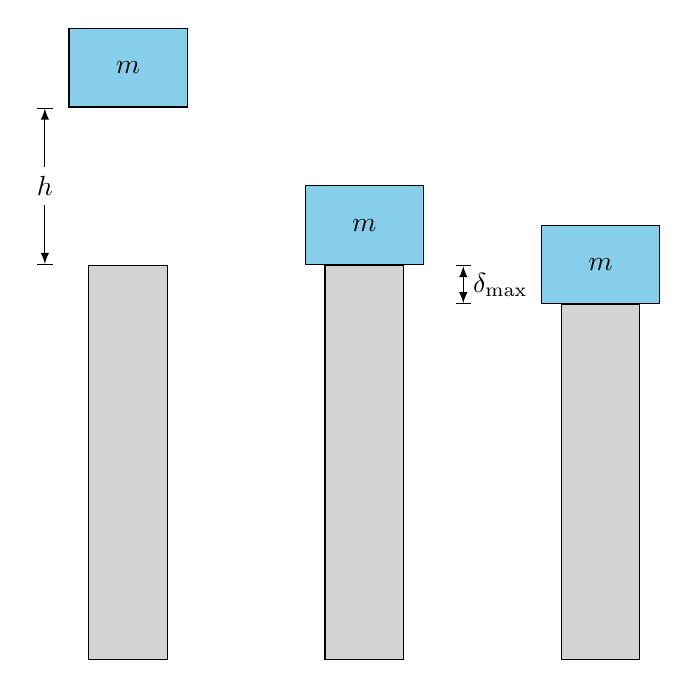
\begin{tikzpicture}
    \node [draw, rectangle, fill=LightGrey, minimum height=5cm, minimum width=1cm](lcol){};
    \node at (lcol.north)[anchor=south, yshift=2cm, draw, rectangle, fill=SkyBlue, minimum height=1cm, minimum width=1.5cm](lbox){$m$};
    \draw [|<->|] (lbox.south west) ++ (180:0.3) --++ (-90:2) node[midway, fill=white]{$h$};
    \node [xshift=3cm, draw, rectangle, fill=LightGrey, minimum height=5cm, minimum width=1cm](mcol){};
    \node at (mcol.north)[anchor=south, draw, rectangle, fill=SkyBlue, minimum height=1cm, minimum width=1.5cm](mbox){$m$};
    \node at (mcol.south) [anchor=south, xshift=3cm, draw, rectangle, fill=LightGrey, minimum height=4.5cm, minimum width=1cm](rcol){};
    \node at (rcol.north)[anchor=south, draw, rectangle, fill=SkyBlue, minimum height=1cm, minimum width=1.5cm](rbox){$m$};
    \draw [|<->|] (mbox.south east) ++ (0:0.5) --++ (-90:0.5) node[midway, right]{$\delta_{\max}$};
  \end{tikzpicture}
  % 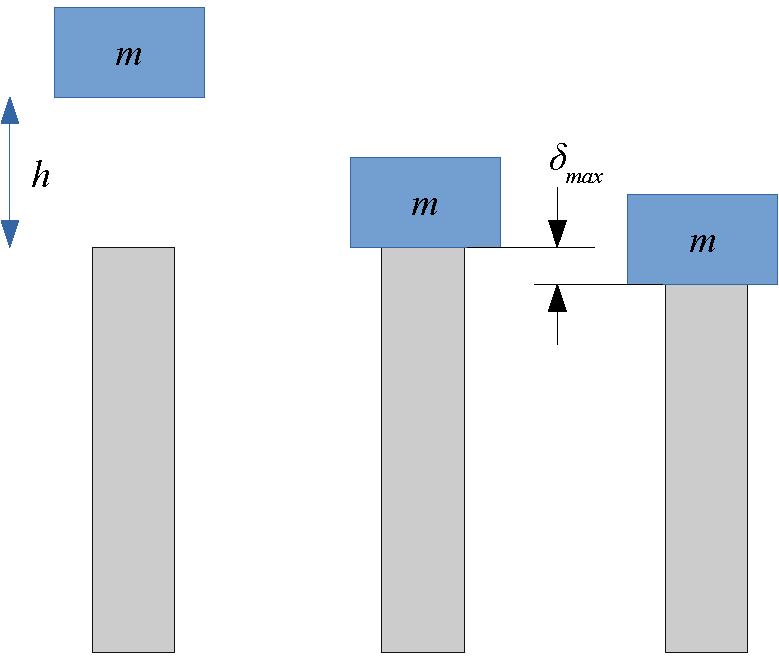
\includegraphics[scale=0.7]{pictures/Axial-load/impact-load}
  \caption{Initial, impact, and maximum deformation conditions in simplified impact loading problem}
  \label{fig: impact loading}
  \end{figure}

  Consider the energy of the system just before the collar is released. The potential energy of the collar with respect to the elevation of the flange is $mgh$, when $g$ is the acceleration of gravity. This potential energy is converted into kinetic energy as the collar falls. At the instant the collar strikes the flange, its potential energy with respect to the elevation is zero and its kinetic energy is $mv^2/2$, where $v = (2gh)^{1/2}$ is its velocity. Following the impact, the kinetic energy is transformed into other forms of energy such as plastic deformation, heat, and sound. However, we will assume that the kinetic energy is wholly transferred to the elastic strain energy in the flange, and that after the collision, the collar `sticks' to the flange as it deforms.

Using these assumptions, we can now calculate the maximum deformation and the stresses produced by the impact load.

\begin{gather}
  mg(h+ \delta_{\max}) = \frac{EA \delta_{\max}^2}{2L} \nonumber \\
  \left( \frac{EA}{2L} \right) \delta_{\max}^2 - mg \delta_{\max} - mgh = 0 \nonumber
\end{gather}

Notice that $mg$ is simply the weight of mass $m$. So let $mg = W$

\begin{align}
  \delta_{\max} = \frac{WL}{EA} + \left[ \left( \frac{WL}{EA} \right)^2 + 2h \left( \frac{WL}{EA} \right) \right]^{1/2}
\end{align}

Notice that $W\mspace{-2mu}L/EA$ is simply the deformation of the bar due to static weight $W$. In other words, $\delta_{st} = W\mspace{-2mu}L/EA$.

\begin{equation}
  \delta_{\max} = \delta_{st} + \left[ \delta_{st}^2 + 2h\delta_{st} \right]^{1/2}
\end{equation}

When $h \gg \delta_{st}$

\begin{equation}
  \delta_{\max} = \sqrt{2h \delta_{st}} = \sqrt{ \frac{mv^2L}{EA} }
\end{equation}

We can similarly show the resultant impact stress, assuming that $\delta = \sigma L / E$

\begin{align}
  \sigma_{\max} &= \frac{\delta_{\max} E}{L} \nonumber \\
                &= \frac{W}{A} + \left[ \left( \frac{W}{A} \right)^2 + 2h \left( \frac{W}{A} \right) \right]^{1/2} \nonumber \\
                &= \sigma_{st} + \left[ \sigma_{st}^2 + 2h \sigma_{st} \right]^{1/2}
\end{align}

And if $h$ is large, then

\begin{equation}
  \sigma_{\max} = \sqrt{ 2h \sigma_{st} } = \sqrt{ \frac{mv^2 E}{AL} }
\end{equation}

Comparison between static and impact responses can be done using the \emph{impact factor}, defined as

\begin{equation}
  \text{impact factor} = \frac{\delta_{\max}}{\delta_{st}} = \frac{\sigma_{\max}}{\sigma_{st}}
\end{equation}

Impact factors can then be used to apply to determine proper design parameters for components under impact loading.

% \begin{example} A battering ram on a castle gate.
  
%   On the final days of Balon Greyjoy's rebellion, the combined armies of Robert Baratheon and Eddard Stark have laid siege on castle on the final Iron Island stronghold of Pyke. Robert ordered his van to ram down the front gate to the castle to commence the final attack. The 500-kg battering ram is a 10-m long solid cylindrical bar made of weirwood with $E$ = 20 GPa and cross sectional radius of 1 m. If the soldiers were able to accelerate the ram up to 20 m/s right before impact, what are the maximum deformation and stress on the ram?
  
%   \begin{center}
%     \begin{tikzpicture}
%       \node [cylinder, draw, minimum height=5cm, minimum width=1cm, inner sep=4](ram){};
%       \node at (ram.east) [anchor=west, xshift=1cm, fill=LightSkyBlue, minimum height=2cm, minimum width=1cm, draw](gate){};
%       \draw [->, ultra thick] (ram.north) ++ (-0.5,0.2) --++ (0:1) node[midway, above]{20 m/s};
%     \end{tikzpicture}
%   \end{center}
  
% \end{example}
% \begin{solution}

%   We can apply the principle of conservation of energy in this problem. Before the impact, the energy of the system is simply the kinetic energy of the ram. At the maximum deformation (and maximum stress) moment, the energy is transferred entirely from the ram to the gate. The gate is 
% \end{solution}

\section*{Summary}

When the deformation of a body in the lateral directions is negligible, its longitudinal deformation can be considered using axially loaded member methodology. First, we consider statically determinate cases, where the use of equilibrium equation is sufficient to determine the deformation of the body. Second, we consider statically indeterminate cases, where, in addition to equilibrium equation, we also need compatibility equation to determine the deformation. From this, we assumed that materials are allowed to deform well into their plastic regimes. After which the removal of the force will lead to permanent deformation and, in certain cases, residual stresses. We then proceeded to relax the assumption that the external force is static, which leads us to impact loading and repeated loading.

\section*{Exercises}

\begin{exercises}

  \item A compound bar consists of four brass wires of 2.5 mm diameter and one steel wire of 1.5 mm diameter. Determine

  \begin{figure}[H]
    \centering
    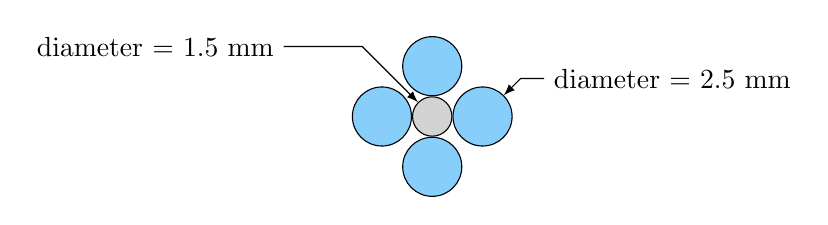
\begin{tikzpicture}
      \node [circle, draw, minimum height=0.5cm, fill=LightGrey](steel){};
      \node at (steel.north) [anchor=south, circle, draw, minimum height=0.75cm, fill=LightSkyBlue]{};
      \node at (steel.east) [anchor=west, circle, draw, minimum height=0.75cm, fill=LightSkyBlue](right){};
      \node at (steel.south) [anchor=north, circle, draw, minimum height=0.75cm, fill=LightSkyBlue]{};
      \node at (steel.west) [anchor=east, circle, draw, minimum height=0.75cm, fill=LightSkyBlue]{};
      \draw [<-] (right.north east) --++ (45:0.3) --++ (0:0.3) node[right]{diameter = 2.5 mm};
      \draw [<-] (steel.north west) --++ (135:1) --++ (180:1) node[left]{diameter = 1.5 mm};
    \end{tikzpicture}
  \end{figure}
  \begin{enumerate}
  \item the stresses in each of the wires when the bar supports a load of 500 N, assuming all the wires are of equal lengths.
  \item The ‘equivalent’ or ‘combined’ modulus for the compound bar and its total extension if it is initially 0.75 m long. 
    For brass $E$ = 100 GPa and for steel $E$ = 200 GPa.
  \end{enumerate}

  \item A compound bar is constructed from three bars 50 mm wide by 12 mm thick fastened together to form a bar 50 mm wide by 36 mm thick. The middle bar is of aluminum alloy for which $E$ = 70 GPa and the outside bars are of brass with $E$ = 100 GPa.

\begin{figure}[H]
      \centering
      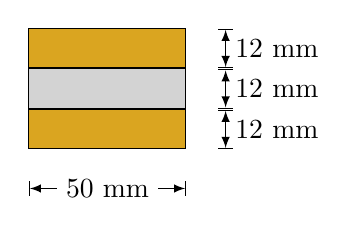
\begin{tikzpicture}
        \node [draw, thin, minimum height=0.5cm, minimum width=2cm, fill=Goldenrod](bottom){};
        \node at (bottom.north) [anchor=south, draw, thin, minimum height=0.5cm, minimum width=2cm, fill=LightGrey](mid){};
        \node at (mid.north) [anchor=south, draw, thin, minimum height=0.5cm, minimum width=2cm, fill=Goldenrod](top){};
        \draw [|<->|] (bottom.south east) ++ (-90:0.5) --++ (180:2) node[midway, fill=White]{50 mm};
        \draw [|<->|] (bottom.south east) ++ (0:0.5) --++ (90:0.5) node[midway, right]{12 mm};
        \draw [|<->|] (mid.south east) ++ (0:0.5) --++ (90:0.5) node[midway, right]{12 mm};
        \draw [|<->|] (top.south east) ++ (0:0.5) --++ (90:0.5) node[midway, right]{12 mm};
      \end{tikzpicture}
    \end{figure}

  \begin{enumerate}
  \item If the bars are initially fastened at 18$\degree$C and the temperature of the assembly is raised to 50$\degree$C, determine the stresses set up in the brass and the aluminum.
        
  \item What will be the changes in these stresses if an external compressive load of 15 kN is applied to the compound bar at the higher temperature?
  \end{enumerate}
    
  \item A composite bar is constructed from a steel rod of 25 mm diameter surrounded by a copper tube of 50 mm outside diameter and 25 mm inside diameter. The rod and tube are joined by two 20 mm diameter pins as shown in the figure below. Find the shear stress in the pins if, after pinning, the temperature is raised by 50 C.

  \begin{figure}[H]
    \centering
    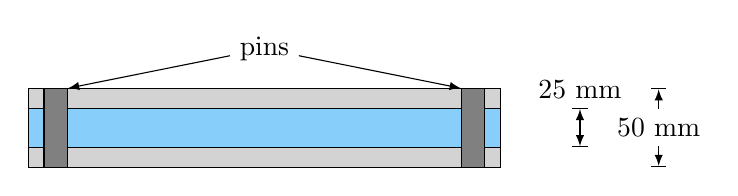
\begin{tikzpicture}
      \node [draw, minimum width=6cm, minimum height=1cm, fill=LightGrey](outer){};
      \node [draw, minimum width=6cm, minimum height=0.5cm, fill=LightSkyBlue](inner){};
      \node at (outer.north west) [anchor=north west, xshift=2mm, draw, minimum width=3mm, minimum height=1cm, fill=Grey](lpin){};
      \node at (outer.north east) [anchor=north east, xshift=-2mm, draw, minimum width=3mm, minimum height=1cm, fill=Grey](rpin){};
      \node at (outer.north) [yshift=5mm](pinnames){pins};
      \draw [<-] (lpin.north east) -- (pinnames);
      \draw [->] (pinnames)-- (rpin.north west);
      \draw [|<->|] (outer.north east) ++ (0:2) --++ (-90:1) node[midway, fill=white]{50 mm};
      \draw [|<->|] (inner.north east) ++ (0:1) --++ (-90:0.5) node[at start, above, fill=white]{25 mm};
    \end{tikzpicture}
  \end{figure}
  For steel $E$ = 210 GPa and $\alpha = 11 x 10^{-6}$ per C
  For copper $E$ = 105 GPa and $\alpha = 17 x 10^{-6}$ per C
  
  \item A rigid beam of length $L$ is pinned to a wall on one side so it is only allow to rotate within the plane of this paper. A spring with constant $k$ is connected to the beam at the middle. If a mass $M$ is falling from height h above on to the end of the beam, prove that the deflection of the end of the beam is equal to

  $$ \delta = \dfrac{4Mg}{k} \left[ 1 + \left( 1 + \dfrac{kh}{2Mg} \right)^{1/2}
  \right] $$

  \begin{figure}[H]
    \centering
    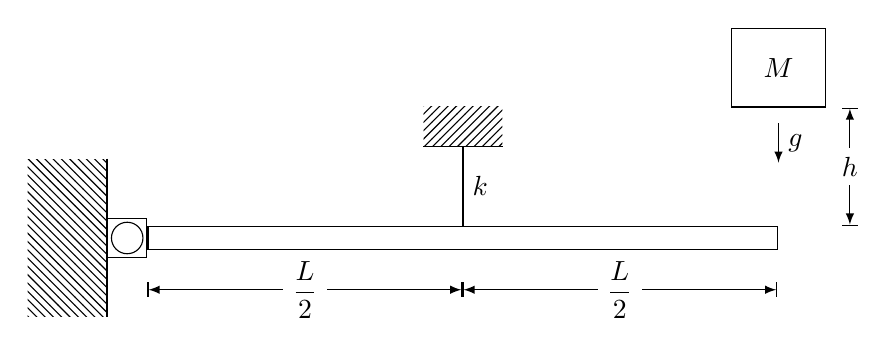
\begin{tikzpicture}
      \node [minimum height=2cm, minimum width=1cm, pattern=north west lines](wall){};
      \draw (wall.north east) -- (wall.south east);
      \node at (wall.east) [anchor=west, minimum height=5mm, minimum width=5mm, draw](hinge){};
      \node at (hinge.center) [circle, minimum height=4mm, draw](pin){};
      \node at (hinge.east) [anchor=west, minimum height=3mm, minimum width=8cm, draw](beam){};
      \draw (beam.north) --++ (90:1) node[midway, right]{$k$} node[anchor=south, minimum height=5mm, minimum width=1cm, pattern=north east lines](ceiling){};
      \draw (ceiling.south east) -- (ceiling.south west);
      \node at (beam.north east) [anchor=south, draw, yshift=1.5cm, minimum height=1cm, minimum width=1.2cm](mass){$M$};
      \draw [->] (mass.south) ++ (-90:0.2) --++ (-90:0.5) node[midway, right]{$g$};
      \draw [|<->|] (mass.south east) ++ (0:0.3) --++ (-90:1.5) node[midway, fill=White]{$h$};
      \draw [|<->|] (beam.south west) ++ (-90:0.5) --++ (0:4) node(A){} node[midway, fill=White]{$\dfrac{L}{2}$};
      \draw [|<->|] (A.center) --++ (0:4) node[midway, fill=White]{$\dfrac{L}{2}$};
    \end{tikzpicture}
  \end{figure}
  
  \item Beam AB is fixed between two walls distance 3 m apart. The beam has a cross-sectional area of 0.1 m$^2$ and the material is elastic-perfectly plastic, has $E$ = 70 GPa, and has a yield stress = 200 MPa. A load $P$ is applied at point C toward point A. Find

  \begin{figure}[H]
    \centering
    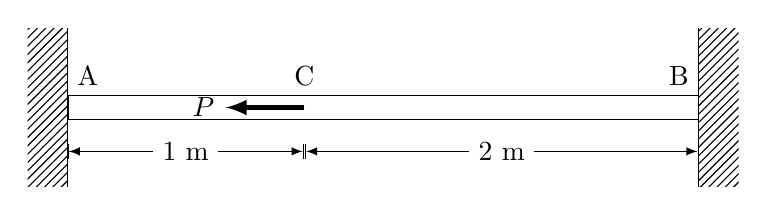
\begin{tikzpicture}
      \node [minimum height=2cm, minimum width=0.5cm, pattern=north east lines](lwall){};
      \draw (lwall.north east) -- (lwall.south east);
      \node at (lwall.east) [anchor=west, draw, minimum height=0.3cm, minimum width=8cm](beam){};
      \node at (beam.east) [anchor=west, minimum height=2cm, minimum width=0.5cm, pattern=north east lines](rwall){};
      \draw (rwall.north west) -- (rwall.south west);
      \node at (beam.north west) [above right]{A};
      \node at (beam.north east) [above left]{B};
      \node at (beam.north) [above, xshift=-1cm]{C};
      \draw [|<->|] (beam.south west) ++ (-90:0.4) --++ (0:3) node[midway, fill=White]{1 m};
      \draw [|<->|] (beam.south east) ++ (-90:0.4) --++ (180:5) node[midway, fill=White]{2 m};
      \draw [->, ultra thick] (beam.center) ++ (180:1) --++ (180:1) node[left]{$P$};
    \end{tikzpicture}
  \end{figure}
  
  \begin{enumerate}
  \item The load $P$ in which both segments will start to yield.
  \item The residual stress in both segments after load $P$ is removed.
  \item The elongation of beam AB after the walls and load $P$ are removed.
  \end{enumerate}

  \item A 2-m long compound cable is used to hoist a weight $W$ up onto a platform. It consists of one steel section and one aluminum section, both with circular cross sections. Steel and aluminum have the following properties: 

  \begin{table}[H]
    \centering
    \begin{tabular}{  c c c }
      \toprule
      Material & Steel & Aluminum \\
      \midrule
      $E$ (GPa) & 210 & 70 \\
      $\sigma_{allow}$ (MPa) & 100 & 50 \\
      $\nu$	&	0.3	&	0.25 \\
      cross section area (mm$^2$) & 80 & 160 \\
      \bottomrule
    \end{tabular}
  \end{table}

  \begin{figure}[H]
    \centering
    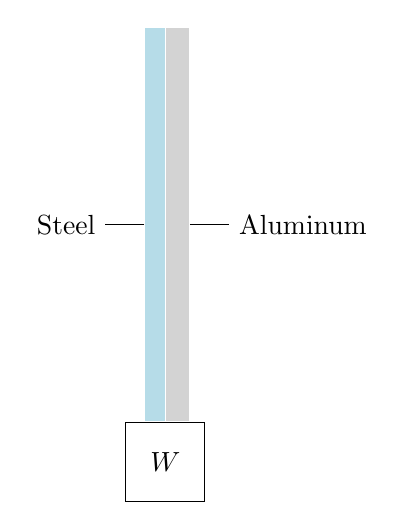
\begin{tikzpicture}
      \node at (0,0) [rectangle, inner sep=0, minimum height=5cm, minimum width=0.25cm, fill=LightBlue!90](A){};
      \node at (A.east) [anchor=west, rectangle, minimum height=5cm, minimum width=0.3cm, fill=LightGrey](B){};
      \node at (A.south east) [anchor=north, draw, rectangle, minimum height=1cm, minimum width=1cm]{$W$};
      \draw (A.west) -- ++(180:0.5) node[left]{Steel};
      \draw (B.east) -- ++(0:0.5) node[right]{Aluminum};
    \end{tikzpicture}
  \end{figure}
  
  \begin{enumerate}
  \item What is the maximum weight $W$ that can be hoisted by the compound cable?
  \item What are the final volumes of both sections when $W$ found in (a) is hoisted?
  \end{enumerate}

\begin{pycode}
E_st = random.randint(15,25)*10*1e9 # 150 - 250 GPa
E_al = random.randint(10,20)*5*1e9 # 50 - 100 GPa
E_cu = random.randint(3,8)*10*1e9 # 30 - 80 GPa

L_st = random.randint(20,30)/10 # 2 - 3 m
L_al = random.randint(15,40)/10 # 1.5 - 4 m
L_cu = random.randint(10,30)/10 # 1 - 3 m

A_st = random.randint(2,5)*1e-4 # 2 - 5 cm2
A_al = random.randint(4,8)*1e-4 # 4 - 8 cm2
A_cu = random.randint(6,10)*1e-4 # 6 - 10 cm2

sigma_st = random.randint(20,45)*10*1e6 # 200 - 450 MPa
sigma_al = random.randint(10,25)*10*1e6 # 100 - 250 MPa
sigma_cu = random.randint(6,15)*10*1e6 # 60 - 150 MPa
\end{pycode}

  \item A compound bar is made up of three materials whose properties and dimensions are as follows

        \begin{table}[htbp]
          \centering
          \begin{tabular}{lcccc}
            \toprule
            Material & $E$ [GPa] & $\sigma_{\text{allow}}$ [MPa] & $L$ [m] & $A$ [cm$^{2}$] \\
            \midrule
            Steel & \py{E_st/1e9} & \py{sigma_st/1e6} & \py{L_st} & \py{A_st/1e-4} \\
            Aluminum & \py{E_al/1e9} & \py{sigma_al/1e6} & \py{L_al} & \py{A_al/1e-4} \\
            Copper & \py{E_cu/1e9} & \py{sigma_cu/1e6} & \py{L_cu} & \py{A_cu/1e-4} \\
            \bottomrule
          \end{tabular}
        \end{table}

        The three materials are mounted side-by-side on a ceiling so that they form a compound bar and would undergo identical deformation. Determine the maximum force $P$ that can be applied to the compound bar.

  \item A 2-m long $6 \times 10$ cm$^2$  railroad track, fixed on both ends, is sitting in the sun. Solar radiation causes the track to heat up by $\Delta T$. The track is made of AISI1023 steel, with the following properties: $\alpha = 12 \times 10^{-6}$ /C, $E = 200$ GPa, and maximum allowable stress $\sigma_{allow} = 50$ MPa.

  \begin{figure}[H]
    \centering
    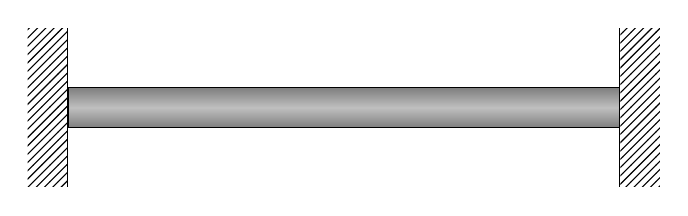
\begin{tikzpicture}
      \node at (0,0) [rectangle, draw, minimum height=0.5cm, minimum width=7cm, top color=Grey, bottom color=Grey, middle color=Grey!50](A){};
      \node at (A.west) [anchor=east, rectangle, minimum height=2cm, minimum width=0.5cm, pattern=north east lines](C){};
      \draw (C.south east) -- (C.north east);
      \node at (A.east) [anchor=west, rectangle, minimum height=2cm, minimum width=0.5cm, pattern=north east lines](B){};
      \draw (B.south west) -- (B.north west);
    \end{tikzpicture}
  \end{figure}
  
  Determine the maximum temperature change $\Delta T$ allowed on the track.
	
\item A 2-m compound bar made of steel and copper is undergoing a heat treatment process for which the materials are heated from 25 C to 300 C. Afterwards, the bar is compressed back by force $P$ until it is back to its original 2-m length while its temperature remains at 300 C. The section properties are as follows:
  
  \begin{table}
    \centering
    \begin{tabular}{ c c c }
      \toprule
      Material	&		Steel	&		Copper \\
      \midrule
      $E$ (GPa)	&	210	&	100	\\
      Cross-sectional area (cm$^2$)	&	20	& 30 \\
      $\alpha$ (/C)	&	10 $\times 10^{-6}$	& 23 $\times 10^{-6}$ \\
      \bottomrule
    \end{tabular}
  \end{table}
  
  \begin{enumerate}
  \item What is the required force $P$?
  \item What are the stresses in the steel and copper sections?
  \end{enumerate}
  
\item A \textbf{1-m} long railroad track is fixed at both ends to the ground. However, when it is fixed, the engineers made a mistake and the fixed ends were only 0.999 m apart. The track is made of steel whose Young's modulus $E$ = 210 GPa and coefficient of thermal expansion $\alpha$ = 13 $\times$ 10$^{-6}$. According to installation standard, the track should  not have more than 300 MPa compressive stress or it will start buckling. How much temperature change can the track take without buckling?

  \begin{figure}[H]
    \centering
    \centering
    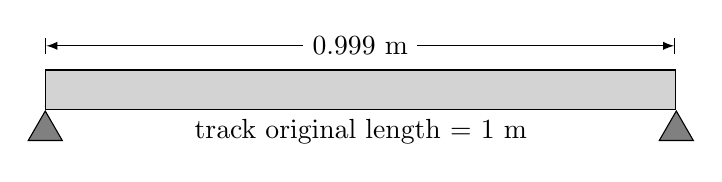
\begin{tikzpicture}[>=latex]
      \node [draw, fill=LightGrey, minimum height=5mm, minimum width=8cm](track){};
      \node at (track.south west) [anchor=north, fill=Grey, draw, regular polygon, regular polygon sides=3, minimum height=5mm, inner sep=0]{};
      \node at (track.south east) [anchor=north, fill=Grey, draw, regular polygon, regular polygon sides=3, minimum height=5mm, inner sep=0]{};

      \draw [|<->|] (track.north west) ++ (90:0.3) --++ (0:8) node[midway, fill=White]{0.999 m};
      \node at (track.south) [below] {track original length = 1 m};
    \end{tikzpicture}
  \end{figure}

\end{exercises}
  %%%%%%%%%%%%%%%%%%%%%%%%%%%%%%%%%%%%%%%%%%%%%%%%%%%%%%%%%%%%%%%%%%%%%%%%%%%%%%%%%%%%%%%%%%%%%%%%%%%%%%%%%%%%%%%%%%%%%%%%%%%%%%%%%%%%%%%%%%%%%%%%%%%%%%%%%%%%%%%%%%%%%%%%%%%%%% 

\chapter{Analysis of Members under Torsion}

Torsion is a twist of a straight bar when loaded by moments that tend to produce rotation about the longitudinal axis of the bar. In this chapter, we begin by developing formulas for the deformations and stresses in circular bars under torsion. We then analyze the rotating shafts and determine the power they transmit. Finally, we cover several additional topics related to torsion such as statically indeterminate members, strain energy, thin-walled tubes, and power transmission.

\section{Simple torsion}

Simple torsion is the case where the cross-sectional area and the torque throughout the length of the material are constant. The understanding of simple torsion and its conditions can be applied to other more complex torsion in upcoming sections.

\subsection{Torsion of circular elastic bars}

When a circular bar is twisted by torques $T$ at the ends, every cross section of the bar is still identical and is subjected to the same internal torque $T$, we say that the bar is in pure torsion. From consideration of symmetry, it can be proved that cross sections of the bar do not change in shape as they rotate about the longitudinal axis. Furthermore, if the angle of rotation between one end of the bar and the other is small, neither the length of the bar nor its radius will change.

\begin{figure}[h]
  \centering
  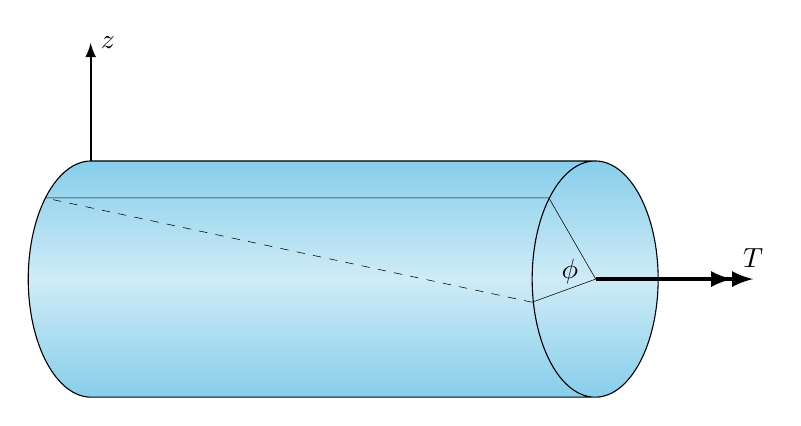
\begin{tikzpicture}
    \draw [->, thick] (0,0) --++ (90:3) node[right]{$z$};
    \node at (0,0) [anchor=west, xshift=-8mm, draw, top color=SkyBlue, bottom color=SkyBlue, middle color=SkyBlue!40, cylinder, minimum height=8cm, minimum width=3cm, inner sep=0.8cm](cyl){};
    \draw [->>, ultra thick] (cyl.east) ++ (180:0.8) node(O){} --++ (0:2) node[above]{$T$};
    \draw [very thin] (O.center) --++ (120:1.19) --++ (180:6.4) node(A){};
    \draw [very thin] (O.center) --++ (200:0.86) node(B){};
    \draw [very thin, dashed] (B.center) -- (A.center);
    \node at (O.center) [left, yshift=1mm, xshift=-1mm] {$\phi$};
  \end{tikzpicture}
  % 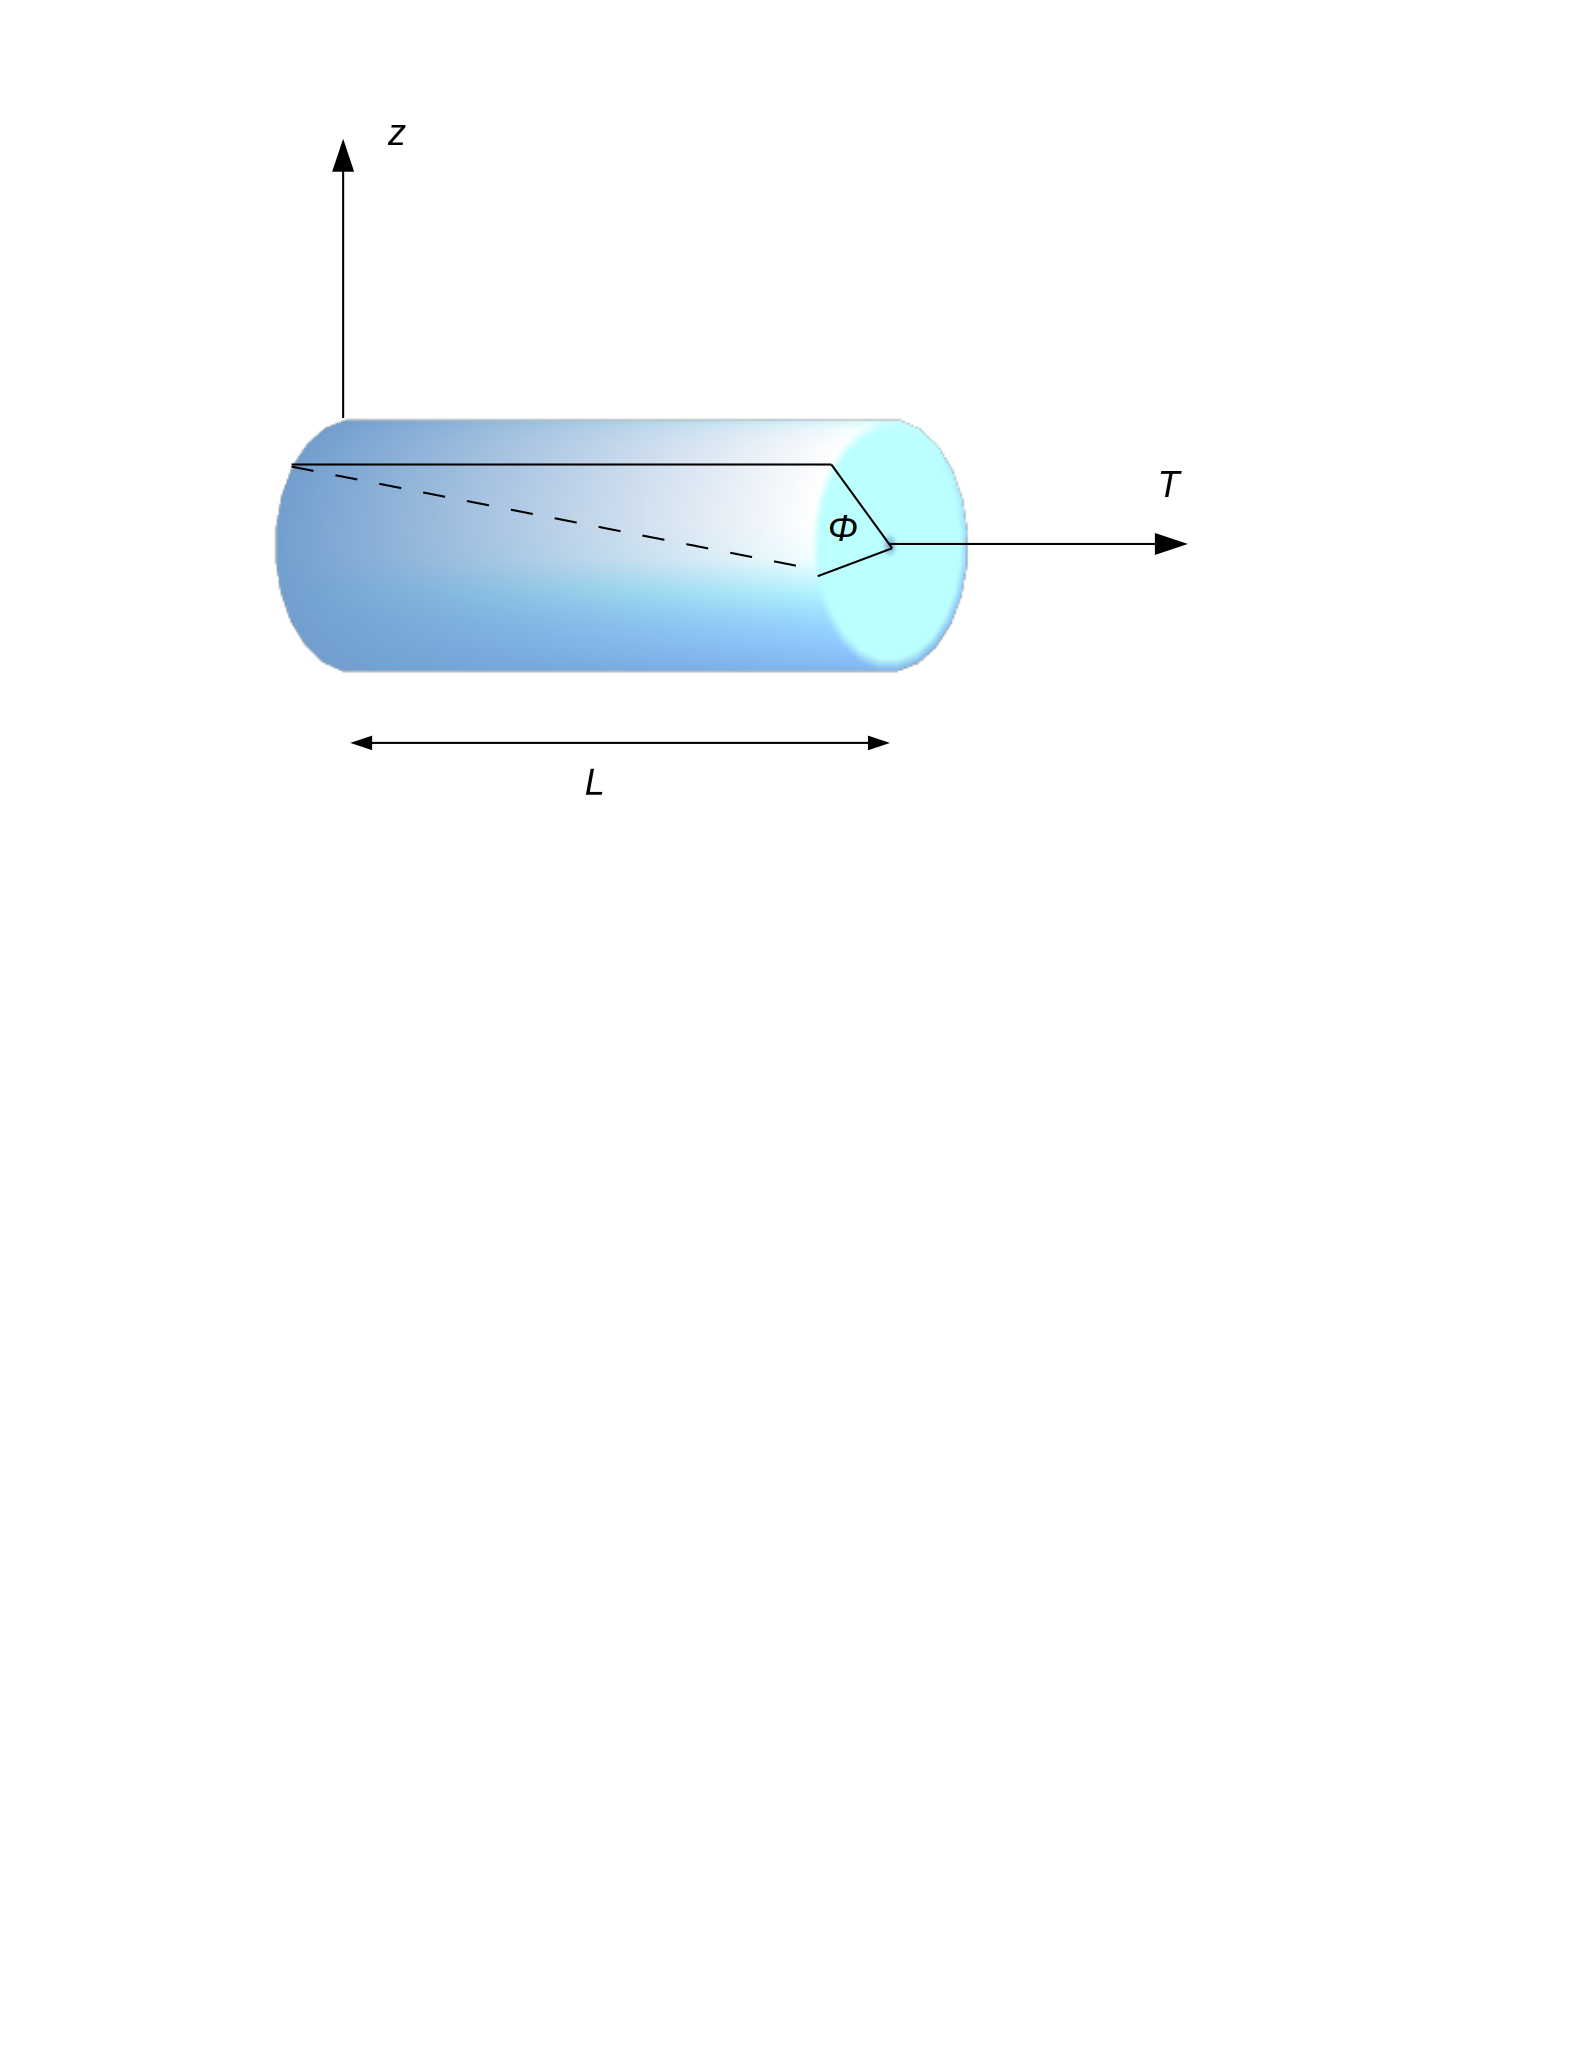
\includegraphics[scale=0.8]{pictures/Static-body-load-analysis/3d-torsion}
  \caption{A circular bar under torsion. The figure shows the torque and deformation on the cross section.}
  \label{fig: 3d torsional deformation}
\end{figure}

Consider a circular bar under torsion in \cref{fig: 3d torsional deformation}. Under the action of torque $T$, if the left-hand end is fixed, the right-hand end will rotate through a small angle $\phi$, known as the angle of twist. The angle of twist changes along the axis of the bar, and at intermediate cross sections it will have a value $\phi(x)$, which we can prove varies linearly between the ends.

\begin{figure}[h]
  \centering
  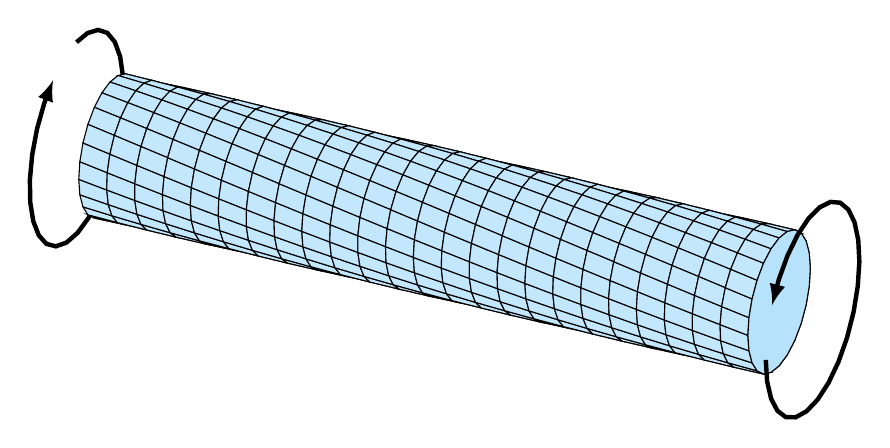
\begin{tikzpicture}
    \begin{axis}[
      scale=2,
      axis equal image, 
      z buffer=sort,
      hide axis, 
      domain=0:1, y domain = 0:10, samples y = 25,
      ylabel =y, xlabel=x,
      clip=false,
      ]

      \addplot3 [
      z buffer=none, domain=0:330, samples y=1,
      ultra thick, black, -latex] (
      -0.5,
      {sin(x)*1.5},
      {cos(x)*1.5}
      );

      \addplot3 [surf, shader=flat corner, fill=LightSkyBlue!50, draw=black] (
      y,
      {cos(360*x) * cos(y*9) - sin(360*x) * sin(y*9)},
      {cos(360*x) * sin(y*9) + sin(360*x) * cos(y*9)}
      );

      \addplot3 [z buffer=none, fill=LightSkyBlue!60, draw=black] (
      10,
      {cos(360*x) * cos(90) - sin(360*x) * sin(90)},
      {cos(360*x) * sin(90) + sin(360*x) * cos(90)}
      );

      \addplot3 [
      z buffer=auto, domain=-60:270, samples y=1,
      ultra thick, black, latex-] (
      10.5,
      {sin(x)*1.5},
      {cos(x)*1.5}
      );
    \end{axis}
  \end{tikzpicture}
  \caption{Surface of a cylindrical shaft under torsion}
\end{figure}

The shear strain in an element of length $dx$ is simply the change in the orientation of the originally straight longitudinal line. The change in the orientation can be defined by the angle of change along the length, which is

\begin{equation} \label{eqn: strain and angle of twist}
  \gamma _{\max } = \frac{{rd\phi }}{{dx}} = r\theta  = \frac{{r\phi }}{L}
\end{equation}

where $\theta$ is defined as the angle of twist per unit length, or rate of twist, and $r$ is the radius of the cross-section. Due to symmetry and our assumption that the cross section remains unchanged during the rotation, the radius of the cross section remains undistorted during this time as well, and therefore the shear strain within the interior of the bar radius away from the center is

\begin{equation} \label{eqn: strain and radius}
  \gamma  = \rho \theta  = \frac{\rho }{r}{\gamma _{\max }}
\end{equation}

Since the bar is in pure shear, we can apply Hooke’s law in shear to analyze the state of stress of the bar in torsion. We have

$$\tau  = G\gamma $$

in which $G$ is the shear modulus of elasticity. We can combine this equation with \cref{eqn: strain and angle of twist} and \cref{eqn: strain and radius} to get

\begin{equation}
  \begin{gathered}
    {\tau _{\max }} = Gr\theta  \hfill \\
    \tau (\rho ) = G\rho \theta  = \dfrac{\rho }{r}{\tau _{\max }} \hfill 
  \end{gathered}
\end{equation}

in which $\tau_{max}$ is the shear stress at the outer surface of the bar and $\tau$ is the shear stress at the interior point of radius $\rho$ from the center of the bar.
Now that we have figured out the stress and strain state in a circular bar under torsion, we will now go on to determine the relationship between the external load (in the case of torsion, the twisting moment or torque T and the shear stress.
First we consider a small element of area $dA$ located at a radial distance $\rho$ from the center of the bar. The shear force acting on the surface would be $\tau dA$ where $\tau$ is the shear stress at radius $\rho$. The moment from the shear force is simply the force times the distance from the center, $\tau \rho dA$. We can express this small moment as

\[dM = \tau \rho dA = \frac{\tau_{\max }}{r}\rho ^2dA\]

The resultant moment is simply the sum of these small moments across the cross-sectional area

\begin{figure}[h]
  \centering
  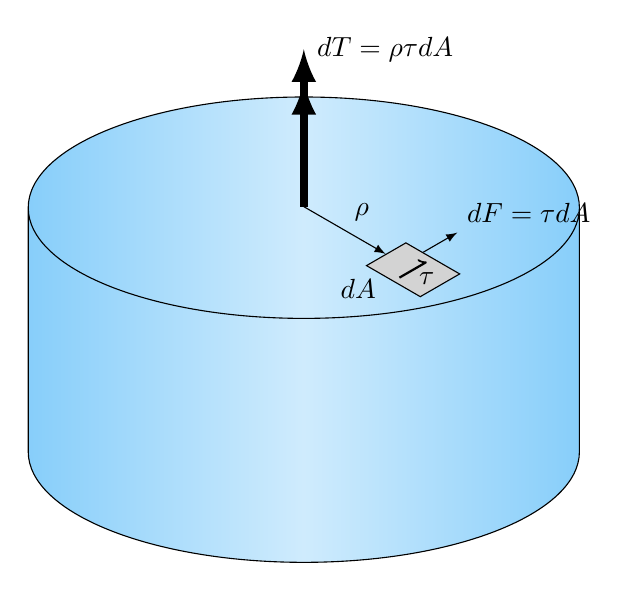
\begin{tikzpicture}[>=latex]
    \node[draw, left color=LightSkyBlue, right color=LightSkyBlue, middle color=LightSkyBlue!40, cylinder, rotate=90, minimum width=7cm, minimum height=3cm, inner sep=40](A){};
    \draw[->>, line width=3pt] (A.top) ++ (0,-1.4) node(B){} --++ (90:2cm) node[right]{$dT = \rho \tau dA$};
    \draw[->] (B.center) --++ (-30:1.2) node(C){} node[midway, above right]{$\rho$} node[below left, yshift=-0.2cm]{$dA$};
    \node at (C) [anchor=west, draw, trapezium, trapezium left angle=60, trapezium right angle=-60, fill=LightGrey, minimum width=5mm, minimum height=5mm, rotate=-30](D){};
    \draw[-left to, thick] (D.center) ++ (-150:0.2) --++(30:0.4) node[below]{$\tau$};
    \draw[->] (D.north) -- ++ (30:0.5) node[above right]{$dF=\tau dA$};
  \end{tikzpicture}
  \caption{Torsion formula derivation.}
\end{figure}

\[T = \int_A {dT}  = \frac{{{\tau _{\max }}}}{r}\int_A {{\rho ^2}dA}  = \frac{{\tau _{\max }}}{r}{J}\]

in which $J$ is the polar moment of inertia of the circular cross section. By rearranging this equation, we obtain the maximum shear stress as a function of applied torque:

\begin{equation} \label{eqn: torsion formula}
  {\tau _{\max }} = \frac{{Tr}}{{{J}}}
\end{equation}

This equation is called the torsion formula. Similar to shear strain, the shear stress at a distance $\rho$ from the center of the bar is

\begin{equation}
  \tau  = \frac{\rho }{r}{\tau _{\max }} = \frac{{T\rho }}{{{J}}}
\end{equation}

Finally, we can also relate the angle of twist of a linearly elastic bar to the applied torque T by combining Hooke’s law in shear and the torsion formula, for which we get

\[\begin{gathered}
    {\tau _{\max }} = Gr\theta \\
    {\tau _{\max }} = \frac{Tr}{J} \hfill \\
    \theta  = \frac{T}{{G{J}}} \hfill \\ 
  \end{gathered} \]

This shows that the rate of twist is directly proportional to the torque $T$ and inversely proportional to the product $GJ$. The total angle of twist for the bar in pure torsion is

\begin{equation}
  \phi  = \theta L = \frac{TL}{GJ} = \frac{T}{k_T}
\end{equation}

where $k_T = GJ/L$ is called the torsional stiffness of the bar.

\begin{example} Statically indeterminate torsional analysis in a cylindrical shaft
  
  A circular bar is supported at both ends by ball bearing hubs, allowing them to rotate freely. Three torques are applied along the length of the bar, their magnitudes, directions, and locations are shown in the figure. The bar has diameter of 3 cm, the material it is made of has G = 80 GPa. Find the maximum shear stress in each segment and angle of twist between point B and D.

  \begin{figure}[H]
  \centering
  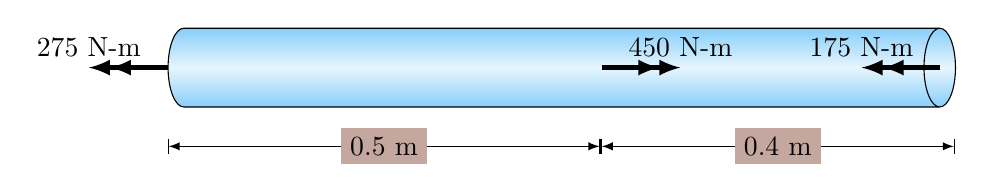
\begin{tikzpicture}
    % \fill [white] (-7,-2) rectangle (6,2);
    \node[draw, top color=LightSkyBlue, bottom color=LightSkyBlue, middle color=LightSkyBlue!20, cylinder, minimum height=10cm, minimum width=1cm, inner sep=2mm](cyl){};
    \draw [->>, ultra thick] (cyl.west) --++ (180:1) node[above]{275 N-m};
    \draw [->>, ultra thick] (cyl.east) ++ (180:0.2) --++ (180:1) node[above]{175 N-m};
    \draw [->>, ultra thick] (cyl.east) ++ (180:4.5) --++ (0:1) node[above]{450 N-m};
    \draw [|<->|] (cyl.west) ++ (-90:1) --++ (0:5.5) node[midway, fill=titlepagecolor!50]{0.5 m};
    \draw [|<->|] (cyl.west) ++ (-90:1) ++ (0:5.5) --++ (0:4.5) node[midway, fill=titlepagecolor!50]{0.4 m};
  \end{tikzpicture}
\end{figure}
  
\end{example}
  
\begin{solution}
First, we need to find the torque in each segment. We can use equation of equilibrium to calculate just that.

Using the method of section, within segment BC,

$$T =  - {T_1} =  - 275\text{ Nm}$$

Within segment CD,

\[T =  - {T_3} = 175\text{ Nm}\]

The maximum shear stress in each segment is at the outer diameter. We have

\[\begin{gathered}
  {\tau _{\max }} = \frac{{Tr}}{{{J}}} = \frac{{2T}}{{\pi {r^3}}} \hfill \\
  {({\tau_{\max }})_{BC}} = \frac{{2(275\text{ Nm})}}{{\pi {{(1.5 \times {{10}^{ - 2}}\text{ m})}^3}}} = 51.9\text{ MPa} \hfill \\
  {({\tau _{\max }})_{CD}} = \frac{{2(175\text{ Nm})}}{{\pi {{(1.5 \times {{10}^{ - 2}}\text{ m})}^3}}} = 33\text{ MPa} \hfill \\ 
\end{gathered} \]

Angle of twist between B and D is the sum of the angles of twist in BC and CD.

\[\begin{gathered}
  \phi_{BD} = \phi_{BC} + \phi_{CD} \hfill \\
  J = \frac{\pi r^4}{2} = \frac{\pi (1.5 \times 10^{-2}\text{ m})^4}{2} = 7.95 \times 10^{-8}\text{ m}^4 \hfill \\
  \phi_{BC} = \frac{T_{BC}L_1}{GJ} = \frac{( - 275\text{ Nm})(0.5\;{\text{m}})}{(80\text{ GPa})(7.95 \times 10^{-8}\text{ m}^4)} =  - 0.0216\text{ rad} \hfill \\
  \phi_{CD} = \frac{T_{CD}L_2}{GJ} = \frac{(175\text{ Nm})(0.4\text{ m})}{(80\text{ GPa})(7.95 \times 10^{-8}\text{ m}^4)} = 0.0110\text{ rad} \hfill \\
  \phi_{BD} =  - 0.0216 + 0.0110 =  - 0.0106\text{ rad} \hfill \\ 
\end{gathered} \]

Therefore, the bar twisted in the same direction as $T_2$ by 0.0106 rad.
\end{solution}

\section{Nonuniform Torsion}

\subsection{Nonuniform Torsion}

In the case of nonuniform torsion, we have loosened the restrictions previously and implicitly imposed on the previous section which are that the bar must be of constant cross section and that the torque throughout the length of the bar must be constant. In this case, we will use the method of sections and apply the principles already explained in the previous section to analyze nonuniform torsion.

To illustrate the procedure, we will divide nonuniform torsion problems into 3 cases.

\begin{enumerate}
\item Bar consisting of constant cross section segments with constant torque throughout each segment. For example, as the figure shows, the bar is made up of three constant cross segments. and throughout each cross section there is a constant torque.
  
  To analyze this problem, we simply use the method of section to determine the torque throughout each cross section. Once the internal torques is determined, we can apply the equations to find the shear stress or the angle o twist in each segment. The total angle of twist of the bar is simply the sum of the angles of twist for all segments. So we have that

  \begin{figure}[h]
    \centering
    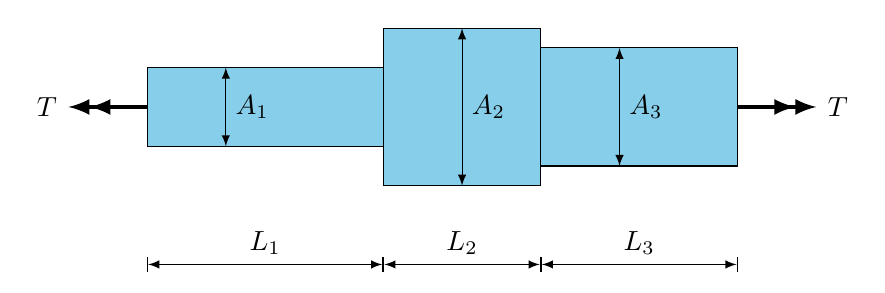
\begin{tikzpicture}
      % members
      \draw[fill=SkyBlue] (0,0) rectangle (3,1) ;
      \draw[fill=SkyBlue] (3,-0.5) rectangle (5,1.5);
      \draw[fill=SkyBlue] (5,-0.25) rectangle (7.5,1.25);
      % extended members
      % force
      \draw[->>, ultra thick] (7.5,0.5) -- (8.5,0.5) node[right]{$T$};
      \draw[->>, ultra thick] (0,0.5) --++ (180:1) node[left]{$T$};
      % lengths
      \draw[|<->|] (0,-1.5) -- (1.5,-1.5) node[above]{$L_1$} -- (3,-1.5);
      \draw[|<->|] (3,-1.5)-- (4,-1.5) node[above]{$L_2$} -- (5,-1.5);
      \draw[|<->|] (5,-1.5)-- (6.25,-1.5) node[above]{$L_3$} -- (7.5,-1.5);
      % areas
      \draw[<->] (1,0) -- (1, 0.5) node[right]{$A_1$} -- (1,1);
      \draw[<->] (4,-0.5) -- (4, 0.5) node[right]{$A_2$} -- (4,1.5);
      \draw[<->] (6,-0.25) -- (6, 0.5) node[right]{$A_3$} -- (6,1.25);
    \end{tikzpicture}
  \end{figure}
  
  \begin{equation}
    \begin{gathered}
      \phi  = {\phi _1} + {\phi _2} + {\phi _3} +  \ldots  \hfill \\
      \phi  = \sum\limits_{i = 1}^n {{\phi _i} = \sum\limits_{i = 1}^n {\dfrac{{{T_i}{L_i}}}{{{G_i}{J_i}}}} }  \hfill \\ 
    \end{gathered}
  \end{equation}
  
  where $i$ indicates the numbering index for various segments.
  
\item Bar with continuously varying cross sections and constant torque. When the torque is constant, the maximum shear stress in a solid bar always occurs at the cross section having the smallest diameter. To find the angle of twist, we can consider an element of length $dx$ at distance $x$ from one end of the bar. The differential angle of twist $\phi$ is
  
  \begin{figure}[h]
    \centering
    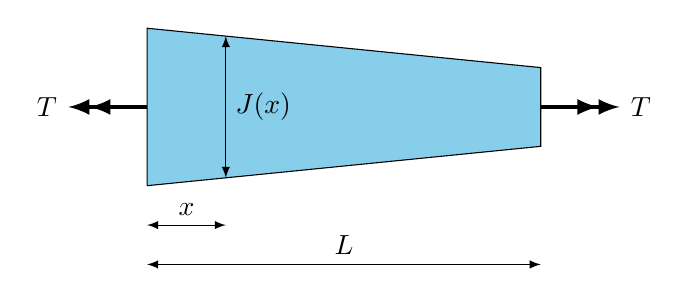
\begin{tikzpicture}
      \draw[fill=SkyBlue] (0,-0.5) -- (5,0) -- (5,1) -- (0,1.5) -- (0,-0.5);
      \draw[->>,ultra thick] (5,0.5) -- (6,0.5) node[right]{$T$};
      \draw[->>,ultra thick] (0,0.5) --++ (180:1) node[left]{$T$};
      \draw[<->] (0,-1.5) -- (2.5,-1.5) node[above]{$L$} -- (5,-1.5);
      \draw[<->] (0,-1) -- (0.5,-1) node[above]{$x$} -- (1,-1);
      \draw[<->] (1,-0.4) -- (1, 0.5) node[right]{$J(x)$} -- (1,1.4);
    \end{tikzpicture}
    \caption{Deformation of a torque-loaded variable cross-sectioned member.}
  \end{figure}
  
  \[d\phi  = \frac{{Tdx}}{{G{J}(x)}}\]
  
  in which $J(x)$ is the polar moment of inertia of cross section at distance x from the end. The angle of twist of the entire bar is the sum of the differential angles of twist:
  
  \begin{equation}
    \phi  = \int_0^L \frac{Tdx}{G{J(x)}}
  \end{equation}
  
  If the expression for the polar moment of inertia is not too complex, the integral can be evaluated analytically; in other cases, however, it must be evaluated numerically.
  
\item Bar with continuously varying cross sections and continuously varying torque. The bar can be subjected to a distributed torque that varies along the length of an also varying cross section bar. We can use the method of sections to find the torque along the length of the bar. We also need to find the polar moment of inertia along the length of the bar. Once we know both quantities, we can use the torsion formula to determine the shear stress. The angle of twist can also be found in the same manner as case 2 except now the torque is also varying. So the equation for the total angle of twist becomes

    \begin{figure}[h]
    \centering
    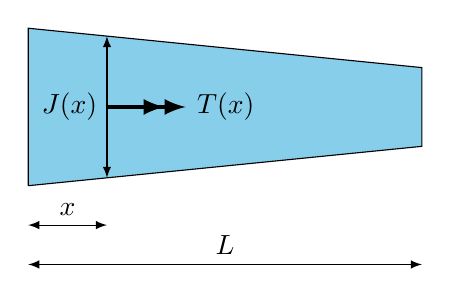
\begin{tikzpicture}
      \draw[fill=SkyBlue] (0,-0.5) -- (5,0) -- (5,1) -- (0,1.5) -- (0,-0.5);
      \draw[->>,ultra thick] (1,0.5) -- (2,0.5) node[right]{$T(x)$};
      \draw[<->] (0,-1.5) -- (2.5,-1.5) node[above]{$L$} -- (5,-1.5);
      \draw[<->] (0,-1) -- (0.5,-1) node[above]{$x$} -- (1,-1);
      \draw[<->] (1,-0.4) -- (1, 0.5) node[left]{$J(x)$} -- (1,1.4);
    \end{tikzpicture}
    \caption{Deformation of a torque-loaded variable cross-sectioned member.}
  \end{figure}
  
  \begin{equation}
    \phi  = \int_0^L \frac{T(x)dx}{G{J(x)}}
  \end{equation}
  
  This integral usually must be evaluated numerically.
\end{enumerate}
  
\section{Statically Indeterminate Members under Torsion}

Similar to axially loaded members, when torque loaded members are constrained against deformation, the torque and deformation in any cross section cannot simply be determined using equilibrium equations alone. Compatibility equations must also be derived and taken into account in order to solve for the deformation and load properly.

\section{Power Transmission}

One of the most common uses of shafts and tubes under torsion is power transmission. When used for this purpose they are subjected to torques that depends on the power generated by the machine and angular speed of the shaft. We can express the power transmitted through a shaft as

\begin{equation}
  P = T\omega
\end{equation}

where $\omega$  is the angular speed of the shaft. For machinery, the frequency of rotation is also often reported. This is a measure of the number of rotations per second. Since one rotation of the shaft covers $2\pi$ radian, then

\begin{equation} \label{eqn: power-torque}
  \begin{gathered}
    \omega  = 2\pi f \hfill \\
    P = 2\pi fT \hfill \\ 
  \end{gathered}
\end{equation}

\begin{example}
  A 40-mm diameter transmission shaft is connected to a motor whose output power is constant at 10 hp.  If the shaft needs to transfer the torque at shaft speed between 100 to 2000 rpm, what is the minimum shear stress the material should be able to withstand?
  
    \begin{figure}[H]
    \centering
    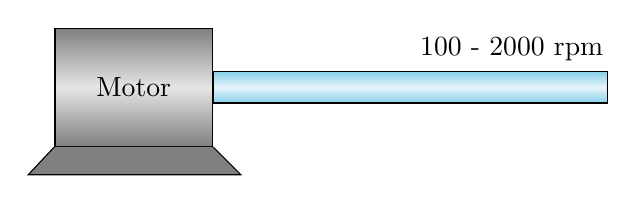
\begin{tikzpicture}
      \node [draw, xshift=1cm, rectangle, top color=SkyBlue, bottom color=SkyBlue, middle color=SkyBlue!20, minimum height=4mm, minimum width=5cm](shaft){};
      \node at (shaft.north) [above right]{100 - 2000 rpm};
      \node at (shaft.west)[anchor=east, draw, rectangle, top color=Grey, bottom color=Grey, middle color=Grey!20, minimum height=1.5cm, minimum width=2cm](motor){Motor};
      \draw [fill=Grey] (motor.south east) --++ (-45:0.5) --++ (180:2.7) -- (motor.south west);
    \end{tikzpicture}
  \end{figure}
  
\end{example}
\begin{solution}
From \cref{eqn: torsion formula}, the maximum shear stress in the shaft occurs when there is maximum torque applied. Using \cref{eqn: power-torque}, we can calculate the maximum torque due to the power transmission. It is evident from the equation that the maximum torque is transferred when the angular speed of the shaft is the lowest. Therefore, the maximum torque applied on the shaft is

\begin{align*}
  P &= 2\pi fT \\ 
  (10 \text{ hp})(746 \text{ W/hp}) &= 2\pi T (100 \text{ rpm})(1/60 \text{ s/min}) \\ 
  T &= 712 \text{ N-m}
\end{align*}	

The maximum shear stress on the material is

\begin{align*}
  {\tau _{\max }} &= \frac{{Tr}}{{{I_p}}} = \frac{{2T}}{{\pi {r^3}}} \\[5pt]
                  &= \frac{2(712 \text{ N-m})}{\pi (20 \times 10^{ - 3})^3} \\[5pt]
                  &= 56.7 \text{ MPa}  
\end{align*}

\end{solution}

\section{Torsion of Thin-walled Tubular Members}

Thin-walled tubes of non-circular shape are often used to construct lightweight frameworks. In some applications, they may be subjected to a torsional loading. In this section, we will analyze the effect of applying a torque to a thin-walled tube having a closed cross section. For this analysis, we will assume that the walls have a variable thickness $t$. Since the walls are thin, we will be able to obtain an approximate solution for the shear stress by assuming that this stress is uniformly distributed across the thickness of the tube. However, we will need to first discuss some preliminary concepts on the action of shear stress over the cross section.

\paragraph{Shear flow.} Consider a small element of a tube along the cross section having a finite length s and differential width $dx$. If the thickness of the tube is nonuniform along the length of the wall, let the thickness on one side be $t_b$ and on the other side be $t_c$. The shear stress on the $b$ side is $\tau_b$ while the stress on the $c$ side is $\tau_c$. Using equation of equilibrium, since the element is in equilibrium, the shear force on one face must be the same in magnitude as the shear force on the opposite face. In other words,

\[F_b = \tau_bt_bdx = \tau_ct_cdx = F_c\]

Since $dx$ is chosen arbitrarily, it follows that the product of shear stress and thickness at any point on the cross section is the same. This product is known as shear flow and is denoted by the letter $f$.

\begin{equation}
  f = \tau_bt_b = \tau_ct_c = \text{constant}
\end{equation}

\paragraph{Shear stress.} The next step is to relate the shear flow and the torque acting on the tube. To do that, consider an element of length $ds$ and thickness $t$. The distance $s$ defining the location of the element is measured along the median line from an arbitrary point. The median line is the line that passes through the middle of the wall thickness along the circumference of the tube.
The total shear force acting on the element is $fds$, and the moment of this force about an arbitrary point $O$ within the tube is

\[dT = rfds\]

In which $r$ is the perpendicular distance from point $O$ to the line of action of the force. The total torque produced by the shear stress is obtained by integrating along the median line.

\[T = f\int_0^{L_m} rds \]

In which $L_m$ denotes the length of the median line. While the integral may seem difficult at first, a simple geometric interpretation helps us evaluate the integral quite easily. $rds$ is twice the area of a triangle formed by $r$ and $ds$. Thus, summing the triangles along the median line gives us the area enclosed by the median line. So the integrals can be written as

\[T = f\int_0^{L_m} rds  = 2fA_m\]

where $A_m$ is the area enclosed by the median line. So we have torsion formula for thin-walled tubes as

\begin{equation} \label{eqn: thin-walled torsion}
  \begin{gathered}
    f = \frac{T}{2A_m} \hfill \\
    \tau  = \frac{T}{2tA_m} \hfill \\ 
  \end{gathered}
\end{equation}

\paragraph{Angle of twist.} The angle of twist can be proven by the energy method, discussed later in this material. If the material is linearly elastic, the angle of twist, $\phi$, can be calculated as

\begin{equation}
  \phi = \frac{TL}{4 A_m^2 G} \oint \frac{ds}{t}
\end{equation}

Note that the line integral has to be performed around the entire median circumference of the cross section.

\begin{example}
  A rectangular tube with thickness of 2 mm throughout is being twisted by a torque. If the tube material has a maximum allowable shear stress of 150 MPa, find the maximum torque that could be applied on the tube.

  \begin{figure}[H]
    \centering
    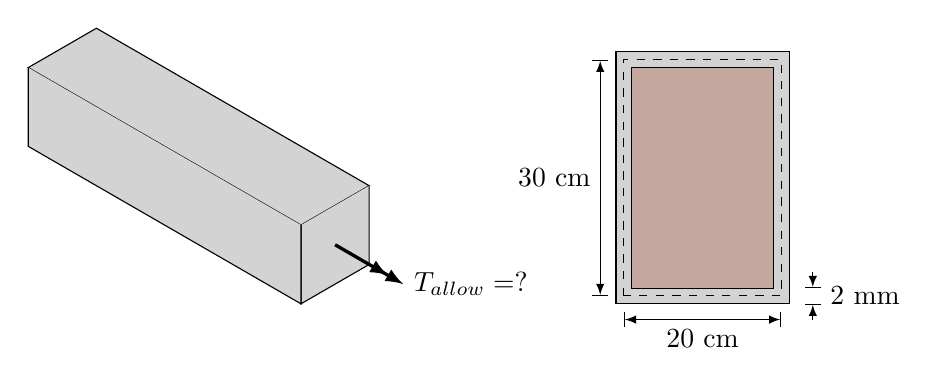
\begin{tikzpicture}[>=latex]
      % grid
      % \draw (-8,-2) grid (8,5);
      % beam
      \draw[fill=LightGrey] (0,0) -- ++ (30: 1cm) -- ++ (150:4) -- ++(-150:1) -- ++ (-30:4);
      \draw[fill=LightGrey] (0,0) -- ++ (-90:1) -- ++ (30:1) -- ++ (90:1);
      \draw[fill=LightGrey] (0,0) -- ++ (-90:1) -- ++ (150:4) -- ++ (90:1);
      % torque
      \draw[->>,very thick] (0.433, -0.25) -- ++ (-30: 1) node[right]{$T_{allow} = ?$};
      % cross section
      \draw[fill=LightGrey] (4, -1) rectangle ++(2.2, 3.2);
      \draw[dashed] (4.1,-0.9) rectangle ++ (2,3);
      \draw[fill=titlepagecolor!50] (4.2,-0.8) rectangle ++(1.8,2.8);
      % dimensioning
      \draw[|<->|] (4.1, -1.2) -- ++ (1, 0) node[below]{20 cm} -- ++ (1,0);
      \draw[|<->|] (3.8, -0.9) -- ++ (90: 1.5) node[left]{30 cm} --++ (90:1.5);
      \draw[->|] (6.5, -0.6) -- ++ (-90:0.2);
      \draw[->|] (6.5, -1.2) -- ++ (90:0.2);
      \draw (6.6, -0.9) node[right]{2 mm};
    \end{tikzpicture}
  \end{figure}
  
\end{example}
\begin{solution}
From \cref{eqn: thin-walled torsion}, we need to first evaluate the area that the median line circumscribes. Since we are given the internal dimensions and thickness, the area circumscribed by the median line is simply the internal dimensions plus half the thickness.

\[\begin{gathered}
    A_m = (0.2 + 0.001 \text{ m})(0.3 + 0.001 \text{ m}) \\ 
    = 0.0605 \text{ m}^2 
  \end{gathered} \]	

After that, finding the maximum allowable torque is simply a matter of substituting all known variables, for which we have

\[\begin{gathered}
  {T_{allow}} = 2t{A_m}{\tau _{allow}} \\ 
   = 2(0.002 \text{ m})(0.0605 \text{ m}^2)(150 \times 10^6 \text{ Pa}) \\ 
   = 36.3 \text{ kN-m} \\ 
\end{gathered} \]
\end{solution}

\section*{Summary}

Torque applied in the direction of the longitudinal axis a body leads to torsion. The problems in torsion are either statically determinate, where the body is unrestrained and can freely deform, and statically indeterminate, where the body is restrained by supports or other materials. The most important application of torsion is power transmission in shaft, in which our knowledge of torsion can help determine and design shafts of appropriate dimensions to meet requirements. Finally, we also learned about approximations and derivations leading to the relationship between torque, deformation, and shear stress in thin-walled tube.

\section*{Exercise}

\begin{exercises}

  \item A solid shaft, 100 mm diameter, transmits 75 kW at 150 rev/min. Determine

  \begin{figure}[H]
    \centering
    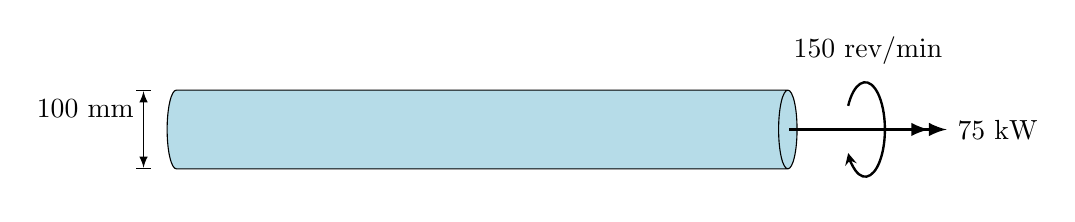
\begin{tikzpicture}[>=latex]
      \node (0,0) [cylinder, draw,fill=LightBlue!90, minimum height=8cm, minimum width=1cm]{};
      \draw[->>, very thick] (4,0) -- ++ (0:2) node[midway]{\AxisRotator} node[right]{75 kW};
      \draw (5,1) node{150 rev/min};
      \draw[|<->|] (-4.2,-0.5) -- ++ (90:1) node[below left]{100 mm};
    \end{tikzpicture}
  \end{figure}
  
  \begin{enumerate}
  \item The value of the maximum shear stress in the shaft and the angle of twist per meter of the shaft length if G = 80 GPa.
  \item The maximum torque the shaft could carry without exceeding the same maximum shear stress, if the shaft has now been bored so that its inner diameter is 60 mm in order to reduce weight.
  \end{enumerate}
  
  \item  Determine the dimensions of a hollow shaft with a diameter ratio of 3:4 which is to transmit 60 kW at 200 rev/min. The maximum shear stress in the shaft is limited to 70 MPa and the angle of twist is 3.8 degree in a length of 4 m. The shaft material has G = 80 GPa.

  \begin{figure}[H]
    \centering
    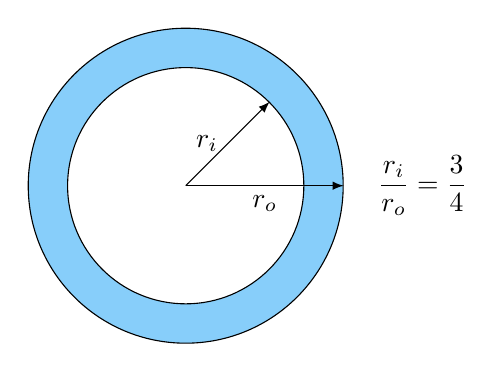
\begin{tikzpicture}
      \node [draw, circle, minimum height=4cm, fill=LightSkyBlue](outer){};
      \node [draw, circle, minimum height=3cm, fill=White](inner){};
      \draw [->] (inner.center) -- (inner.north east) node[midway, left]{$r_i$};
      \draw [->] (outer.center) -- (outer.east) node[midway, below]{$r_o$};
      \node at (outer.east) [xshift=1cm] {$\dfrac{r_i}{r_o} = \dfrac{3}{4}$};
    \end{tikzpicture}
  \end{figure}

  \item A circular bar ABC, 3 m long, is rigidly fixed at its ends A and C. The portion AB is 1.8 m long and of 50 mm diameter and BC is 1.2 m long and of 25 mm diameter. If a twisting moment of $T$ = 680 Nm is applied at B, determine the values of the resisting moments at A and C and the maximum stress in each section of the shaft. What will be the angle of twist of each portion? The shaft material has $G$ = 80 GPa.

  \begin{figure}[H]
    \centering
    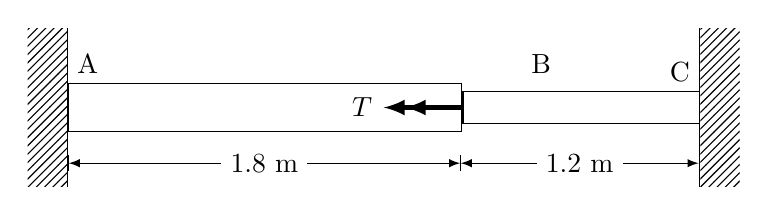
\begin{tikzpicture}
      \node [minimum height=2cm, minimum width=0.5cm, pattern=north east lines](lwall){};
      \draw (lwall.north east) -- (lwall.south east);
      \node at (lwall.east) [anchor=west, draw, minimum height=0.6cm, minimum width=5cm](beam){};
      \node at (beam.east) [anchor=west, draw, minimum height=0.4cm, minimum width=3cm](beam1){};
      \node at (beam1.east) [anchor=west, minimum height=2cm, minimum width=0.5cm, pattern=north east lines](rwall){};
      \draw (rwall.north west) -- (rwall.south west);
      \node at (beam.north west) [above right]{A};
      \node at (beam1.north east) [above left]{C};
      \node at (beam.north east) [above, xshift=1cm]{B};
      \draw [|<->|] (beam.south west) ++ (-90:0.4) --++ (0:5) node[midway, fill=White]{1.8 m};
      \draw [|<->|] (beam1.south east) ++ (-90:0.5) --++ (180:3.05) node[midway, fill=White]{1.2 m};
      \draw [->>, ultra thick] (beam.east) --++ (180:1) node[left]{$T$};
    \end{tikzpicture}
  \end{figure}

\begin{pycode}
L1 = random.randint(3,10)/10 # 0.3 - 1.0 m
L2 = random.randint(5,15)/10 # 0.5 - 1.5 m
x = L1 + L2/random.randint(2,4)
d1 = random.randint(20,40)/10*1e-2 # 2.0 - 4.0 cm
d2 = d1 + random.randint(5,15)/10*1e-2
G = random.randint(5,10)*10*1e9 # 50 - 100 GPa
tau_allow = random.randint(6,12)*10*1e6 # 60 - 120 MPa
phi_allow = random.randint(1,5)/10 # 0.1 - 0.5 rad
\end{pycode}

  \item A two-segment circular cross-sectioned shaft is fitted with a gear at length $x$ = \py{round(x,3)} m. The smaller segment to the left has $L_{1}$ = \py{L1} m and $d_{1}$ = \py{round(d1/1e-2,1)} cm, while the larger segment to the right has $L_{2}$ = \py{L2} m and $d_{2}$ = \py{round(d2/1e-2,1)} cm. Both segments are made of a single material whose $G$ = \py{G/1e9} GPa. For this mechanism to work, the designed allowable shear stress $\tau_{\text{allow}}$ = \py{tau_allow/1e6} MPa and allowable angle of twist $\phi_{\text{allow}}$ = \py{phi_allow} rad. Determine the maximum torque $T$ that the gear can transmit without exceeding $\tau_{\text{allow}}$ or $\phi_{\text{allow}}$.

        \begin{figure}[htbp]
          \centering
          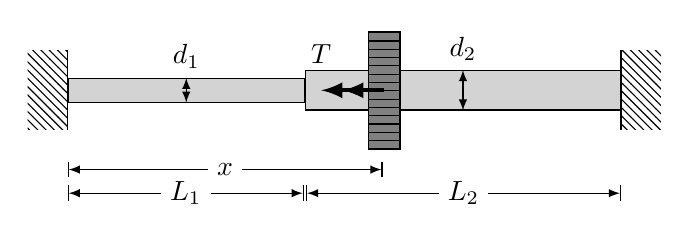
\begin{tikzpicture}[>=latex]
            \node[minimum height=1cm, minimum width=5mm, pattern=north west lines](lwall){};
            \draw (lwall.north east) -- (lwall.south east);
            \node at (lwall.east) [draw, fill=LightGrey, anchor=west, minimum height=3mm, minimum width=3cm](lbeam){};
            \node at (lbeam.east) [draw, fill=LightGrey, anchor=west, minimum height=5mm, minimum width=4cm](rbeam){};
            \node at (rbeam.east) [anchor=west, minimum height=1cm, minimum width=5mm, pattern=north west lines](rwall){};
            \draw (rwall.north west) -- (rwall.south west);
            \node at (rbeam.center) [xshift=-1cm, draw, minimum height=1.5cm, minimum width=4mm, fill=Grey](gear){};
            \node at (rbeam.center) [xshift=-1cm, draw, minimum height=1.5cm, minimum width=4mm, pattern=horizontal lines]{};

            %%%%% Dimensions %%%%%
            \draw [|<->|] (lwall.south east) ++ (-90:0.5) --++ (0:4) node[midway, fill=White]{$x$};
            \draw [|<->|] (lwall.south east) ++ (-90:0.8) --++ (0:3) node[midway, fill=White]{$L_{1}$};
            \draw [|<->|] (rwall.south west) ++ (-90:0.8) --++ (180:4) node[midway, fill=White]{$L_{2}$};
            \draw [<->] (lbeam.south) -- (lbeam.north) node[above]{$d_{1}$};
            \draw [<->] (rbeam.south) -- (rbeam.north) node[above]{$d_{2}$};

            %%%% Torque %%%%%
            \draw [->>, ultra thick] (gear.center) --++ (180:0.8) node[above, yshift=2mm]{$T$};
          \end{tikzpicture}
        \end{figure}

  \item An engineer is working on designing a new electric car model. He planned to reuse the shaft from an old model which uses a gasoline (benzene) engine. The old shaft radius was the minimum that can still operate with the engine, whose power output (in Watt) follows the function
	$$ P_{engine} = -2\times10^{-6} (rpm)^3 + 1.5 \times 10^{-2} (rpm)^2; 1000 < rpm < 6000 $$ 
  where $rpm$ is the engine speed in revolutions per minute. The new electric car uses a motor for which its power output in Watt varies with its angular velocity as
	$$ P_{motor} = -3 \times 10^{-6}(rpm)^3 + 2.5 \times 10^{-2} (rpm)^2; 1000 < rpm < 6000 $$

  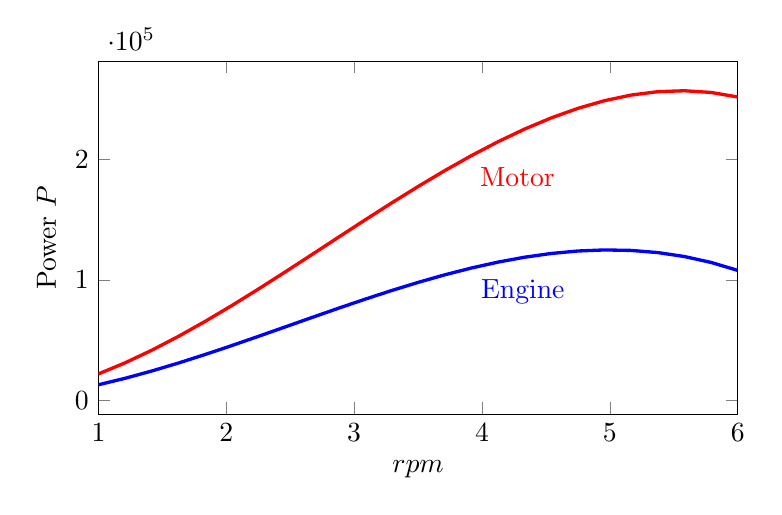
\begin{tikzpicture}
    \centering
    \begin{axis}[
      width=0.8\textwidth,
      height=.5\textwidth,
      xmin=1,xmax=6,
      xlabel={$rpm$},
      ylabel={Power $P$},
      ]
      \addplot [very thick, blue, domain=1:6]{-2*10^3*x^3 + 1.5*10^4*x^2} node[near end, below right]{Engine};
      \addplot [very thick, red, domain=1:6]{-3*10^3*x^3 + 2.5*10^4*x^2} node[near end, below right]{Motor};
    \end{axis}
  \end{tikzpicture}
  
  Is it safe the use the old shaft? Show your work. If not, what should the radius of the new shaft be? Assume that the old and new shafts are manufactured from the same material (AISI 1023), whose $\tau_{allow}$ = 200 MPa.
        
\item  A shaft is fitted with a gear as shown in the picture. The gear is connected to an engine whose maximum torque is provided when it is running at 1000 rpm, giving the power output of 150 kW.

%   $$ P = -2 \cdot 10^{-6} \omega^3 + 1.5 \cdot 10^{-4} \omega^2 $$
% where $0 \leqslant \omega \leqslant 600 $ rad/s

  The shaft is connected with one wheel at each end which can be considered as a fixed end in this problem. The shaft is made of steel whose $\sigma_{\text{allow}}$ = 200 MPa. Determine the minimum required radius of the shaft.

  \begin{figure}[H]
    \centering
    \centering
    \begin{tikzpicture}[>=latex]
      \node [draw, fill=LightGrey, minimum height=5mm, minimum width=6cm](shaft){};
      \node [draw, fill=Grey, minimum width=3mm, minimum height=2cm, xshift=-1cm](gear){};
      % \draw [->>, ultra thick] (gear.center) --++ (0:1) node[below, yshift=-2mm]{$T(\omega)$};
      \draw [<-] (gear.south) --++ (-90:0.5) --++ (0:1) node[right]{gear connected to engine output};
      \node at (shaft.west) [anchor=east, pattern=north west lines, minimum height=2cm, minimum width=0.7cm](wwall){};
      \node at (shaft.east) [anchor=west, pattern=north west lines, minimum height=2cm, minimum width=0.7cm](ewall){};
      \draw (wwall.north east) -- (wwall.south east);
      \draw (ewall.north west) -- (ewall.south west);
      \draw [|<->|] (wwall.north east) ++ (90:0.3) --++ (0:2) node[midway, fill=White]{0.6 m};
      \draw [|<->|] (wwall.north east) ++ (90:0.3) --++ (0:2) node(A){} node[midway, fill=White]{0.6 m};
      \draw [|<->|] (A.center) --++ (0:4) node[midway, fill=White]{1.2 m};
    \end{tikzpicture}
  \end{figure}
\end{exercises}

%%%%%%%%%%%%%%%%%%%%%%%%%%%%%%%%%%%%%%%%%%%%%%%%%%%%%%%%%%%%%%%%%%%%%%%%%%%%%%%%%%%%%%%%%%%%%%%%%%%%%%%%%%%%%%%%%%%%%%%%%%%%%%%%%%%%%%%%%%%%%%%%%%%%%%%%%%%%%%%%%%%%%%%%%%%%%%%%%%%%%%%%%%%%%%%%%%%%%%%%%%%%%%%%%%%%%%%%%%%%%%%%%

\chapter{Analysis of Beam Bending}

When external load is applied perpendicular to the axis of the length of the beam, it will create a shear force and/or bending moment inside the beam. The deformation from this type of load is called deflection. In this chapter, we will analyze the relationship between the external load, the shear force, the bending moment, and the deflection of the beam.

\section{Symmetric Beam Bending}

First we will consider the simplest case of bending where the cross section of the beam in consideration has at least one axis of symmetry, and that the applied load is in the same plane as the axis of symmetry. This will cause bending in the plane of symmetry, resulting in symmetric beam bending.

\subsection{Longitudinal strains in beams}

The longitudinal strain in a beam can be found by analyzing the curvature of the beam and the associated deformations. For this purpose, let us consider a portion ab of a beam in pure bending subjected to positive bending moment $M$. Under the action of the bending moments, the beam deflects in the $xy$ plane and its longitudinal axis is bent into a circular curve. Cross sections of the beam are assumed to remain plane and normal to the longitudinal axis.

\begin{figure}[h]
  \centering
  \begin{tikzpicture}
    \node at (0,0) (O){} node[right]{$O$};
    \draw [dashed] (O.center) -- ++(-120:5) node(A){};
    \draw [line width=40pt, LightSkyBlue] (A.center) arc (-120:-60:5) node(B){};
    \draw [dash dot] (A.center) arc (-120:-60:5) node[near end](y){};
    \draw [->] (y.center) --++ (105:0.3) node[midway, left]{$y$};
    \draw [dashed] (B.center) -- (O.center);
    \draw [<->, black!50] (O.center) ++ (90:1) --++ (-90:8);
    \draw [<->, black!50] (O.center) ++ (-90:5) ++ (180:4) --++ (0:8) node[below, black]{$x$};
    \draw [->] (O.center) --++ (-70:5) node[midway, left]{$\rho$};
    \draw [dashed] (O.center) --++ (-100:5) node[midway, left, yshift=-2mm]{$d\theta$};
    \draw [dashed] (O.center) --++ (-110:5);
  \end{tikzpicture}
 % 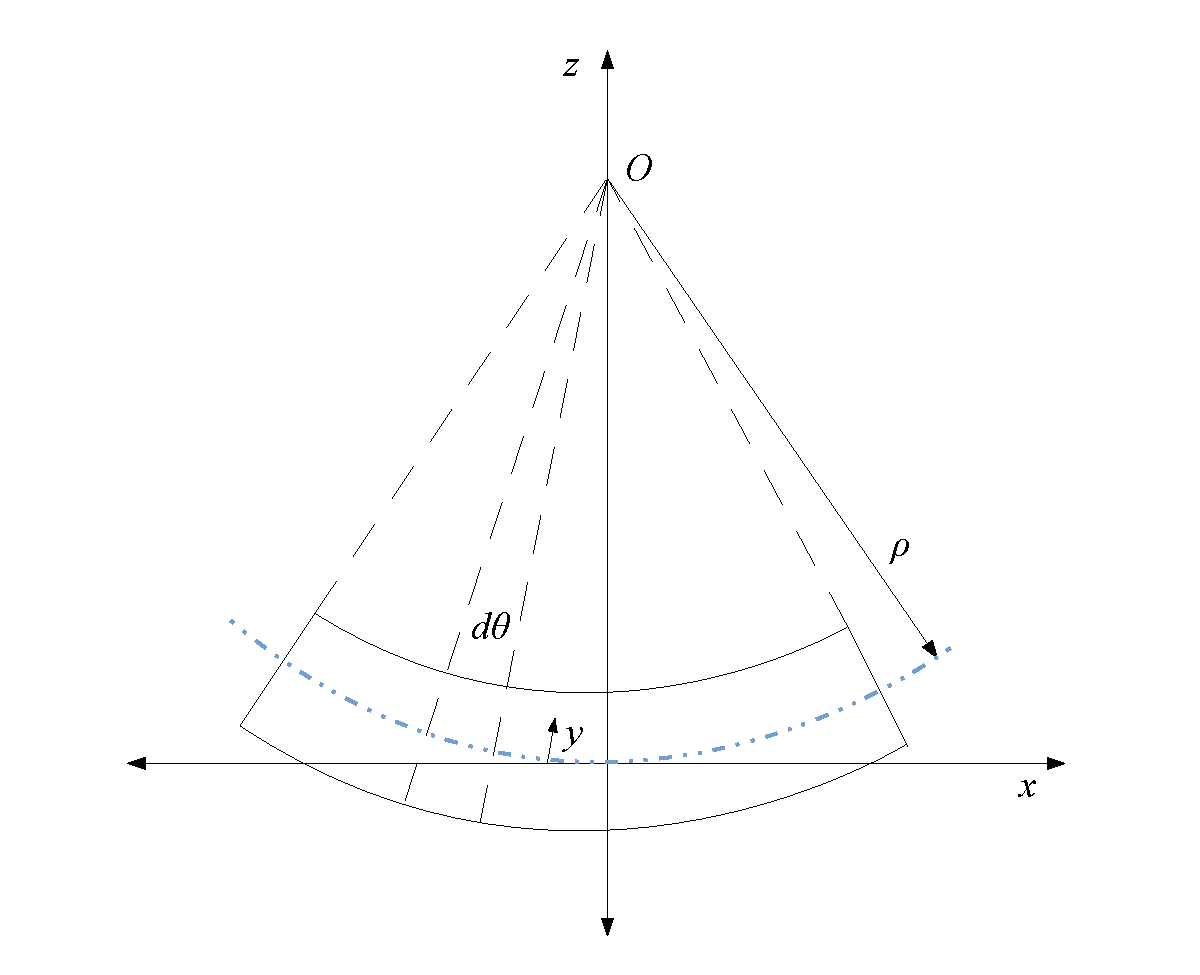
\includegraphics[scale=0.6]{pictures/Static-body-load-analysis/pure-bending}
  \caption{Deformation in pure beam bending.}
  \label{fig: pure bending}
\end{figure}

Because of the bending deformations, cross sections rotate with respect to each other about axes perpendicular to $xy$ plane. As shown in \cref{fig: pure bending}, longitudinal lines of the convex part of the beam are elongated, while those on the concave side are shortened. Therefore, the lower part of the beam is in tension while the upper part is in compression. Somewhere between the top and bottom surface there is a surface where its longitudinal lines do not change in length. This surface is called the \emph{neutral surface}. Its intersection with any cross-sectional plane is called the neutral axis of the cross section.

The planes containing cross sections intersect in a line through the center of curvature. The angle between the two planes is denoted $d\theta$ and the distance to the neutral surface is the radius of curvature $\rho$. The initial distance between the two planes is unchanged at the neutral surface and thus $\rho d \theta = dx$. However, all other lines not on the internal surface either lengthen or shorten, creating normal strains.

To evaluate the normal strains, consider a longitudinal line located at a
distance y away from the neutral surface in an initially straight beam. Once the beam deflects, the neutral surface moves with the beam, but the x axis remains fixed and therefore the longitudinal line is still located at the same distance y away. The new length of this longitudinal line becomes

\[(\rho  - y)d\theta  = dx - \dfrac{y}{\rho }dx\]

Therefore, the corresponding normal strain of this longitudinal line is simply the change in length divided by the original length, which is

\begin{equation}
  {\varepsilon _x} = \frac{{dx - \dfrac{y}{\rho }dx - dx}}{{dx}} =  - \dfrac{y}{\rho } =  - \kappa y
\end{equation}

where $\kappa$ is the curvature.

Note the negative sign in the equation; when the point of interest is above the neutral surface, the part is in compression, and vice versa.

The next step in our analysis is to find the stresses from the strains, which derive from Hooke’s law for linearly elastic materials.

\subsection{Normal stresses in beams}

Since we have established the relationship between the distance of the point of interest from the neutral surface and the normal strain in bending beam, we can now apply Hooke’s law for linearly elastic material to derive the stress in the beam.

\begin{figure}[h]
  \centering
  \begin{tikzpicture}[>=latex]
    \draw [fill=SkyBlue] (0,0) arc [radius=9, start angle=120, end angle=90] --
    ++(90:2) arc [radius=11, start angle=90, end angle=120] -- (0,0);
    \draw[->, thick] (-1.5,2) arc (135:250:1.5cm);
    \draw[dashed, thin] (-0.5,0.866) arc (120:90:10cm);
    \foreach \x in {0,...,10}
    \draw[->] (4.5,3.2 - 0.2*\x) -- ++(0: 1-0.2*\x);
    \draw[->, thick] (6, 3.5) arc (60:-60:1.5);
    \draw (-2.5,1) node{$M$};
    \draw (7, 2.5) node{$M$};
    \draw (5.4,3.1) node[right]{$+\sigma$};
    \draw (3.6,1.4) node[left]{$-\sigma$};
  \end{tikzpicture}
  \caption{Bending stress in uniform bending.}
\end{figure}

\begin{equation} \label{eqn: stress-strain bending}
  {\sigma _x} = E{\varepsilon _x} =  - E\frac{y}{\rho } =  - E\kappa y
\end{equation}

This equation shows that the normal stresses, just like normal strains, vary linearly with the distance $y$ from the neutral surface. For example, when the bending moment $M$ is positive and the beam bends with positive curvature, the stresses are negative (compression) above the neutral surface and positive (tension) below it.

However, in order for \cref{eqn: stress-strain bending} to be useful, we must first determine the location of the neutral axis on the cross section so that we may find the distance of the point of interest from it.

The location of the neutral axis can be determined by employing a static equilibrium equation. We know that the resultant force on any cross section of the beam is zero. We may then apply \cref{eqn: stress-strain bending} using this fact, thus we have

\[\int_A {{\sigma _x}dA}  =  - \int_A {E\kappa ydA}  = 0\]

Since the curvature and the modulus of elasticity are constants at any cross section of the beam, we have

\begin{equation}
  \int_A {ydA}  = 0
\end{equation}

This equation states that the first moment of the area of the cross section, evaluated with respect to the neutral axis, is zero. In other words, the neutral axis must pass through the centroid of the cross section.

\subsection{Moment-curvature formula}

We also know that the resultant moment of the normal stresses acting over the cross section must be equal to the bending moment at that cross section. Let us first consider the element of force $\sigma xdA$ acting on the element of area $dA$ is in the positive direction when $\sigma_x$ is positive. If the element $dA$ is located above the neutral axis, a positive stress would produce an element of moment in $\sigma_xydA$ the negative direction since it tends to bend the beam downward. Therefore, we have

\[dM =  - {\sigma _x}ydA\]

The sum of all the elemental moments of the entire cross section is simply the bending moment:

\[M =  - \int_A {{\sigma _x}ydA} \]

By substituting $\sigma_x = -E\kappa y$, we have

\[M =  - \int_A {\kappa E{y^2}dA}  =  - \kappa E\int_A {{y^2}dA} \]

which we can define as

\begin{figure}[h]
  \centering
  \begin{tikzpicture}[>=latex]
    \draw [fill=SkyBlue] (0,0) arc [radius=9, start angle=120, end angle=90] --
    ++(90:2) arc [radius=11, start angle=90, end angle=120] -- (0,0);
    \draw[dashed, thin] (-0.5,0.866) arc (120:90:10cm);
    \foreach \x in {1}
    \draw[->] (4.5,3.2 - 0.2*\x) -- ++(0: 1-0.2*\x);
    \draw[->, thick] (6, 3.5) arc (75:-75:0.6);
    \draw[|<->|] (4.3,2.2) -- (4.3, 3.0) node[below left]{$y$};
    \draw (6.5, 3) node[right]{$dM = \sigma y dA$};
    \draw (5.3,3) node[above]{$\sigma dA$};
  \end{tikzpicture}
  \caption{Infinitessimal bending moment $dM$ generated from force $\sigma dA$ with a distance $y$ from the neutral axis.}
\end{figure}


\[\begin{gathered}
  M = \kappa EI \hfill \\
  I = \int_A {{y^2}dA}  \hfill \\ 
\end{gathered} \]

where $I$ is called the moment of inertia. We can now rearrange equation 3.43 in terms of the bending moment as

\begin{equation} \label{eqn: moment-curvature}
  \kappa  = \frac{1}{\rho } = \frac{M}{{EI}}
\end{equation}

This equation is known as the moment-curvature equation, showing that the curvature of the bending beam is directly proportional to the bending moment and inversely proportional to the quantity $EI$, which is called the \emph{flexural rigidity} of the beam.

\subsection{Elastic Flexure Formula}

Now that we have located the neutral axis and derived the moment-curvature relationship, we can determine the stress inside the beam from the bending moment. Substituting \cref{eqn: moment-curvature} into \cref{eqn: stress-strain bending}, we have

\begin{equation} \label{eqn: flexure formula}
  {\sigma _x} =  - \frac{{My}}{I}
\end{equation}

This equation is called the flexure formula, shows that the stresses are directly proportional to the bending moment $M$ and inversely proportional to the moment of inertial $I$. The stresses also vary linearly with the distance $y$ from the neutral axis.

\subsection{Maximum stress at a cross section}

From \cref{eqn: flexure formula}, we know that the maximum tensile stress and compressive stress on a given cross section occurs at points located the furthest away from the neutral axis. Assume the distance from the neutral axis to the extreme elements above and below to be $c_1$ and $c_2$ respectively, then the corresponding maximum normal stresses from the flexure formula are

\begin{equation} \label{eqn: section modulus}
  \begin{gathered}
    \sigma _1 =  - \frac{Mc_1}{I} =  - \frac{M}{S_1} \hfill \\
    \sigma _2 =  - \frac{Mc_2}{I} =  - \frac{M}{S_2} \hfill \\ 
  \end{gathered}
\end{equation}

in which

\[\begin{gathered}
  S_1 = \frac{I}{c_1} \hfill \\
  S_2 = \frac{I}{c_2} \hfill \\ 
\end{gathered} \]

The quantities $S_1$ and $S_2$ are known as the section moduli of the cross section.

\begin{example}
  A rectangular cross-sectioned beam is put under 3 point loading scheme as shown. Its cross-sectional width is 3 cm and height is 5 cm. Determine the maximum stress in the beam.

  \begin{figure}[H]
    \centering
    \begin{tikzpicture}[>=latex]
      % \node [rectangle, fill=white, minimum height=4cm, minimum width=10cm]{};
      \node [draw, rectangle, fill=SkyBlue, minimum width=8cm, minimum height=2mm](beam){};
      \node at (beam.south west)[anchor=north, xshift=1cm, draw, fill=LightGray, circle, minimum height=3.9mm, inner sep=0](left){};
      \node at (beam.south east)[anchor=north, xshift=-1cm, draw, fill=LightGray, regular polygon, regular polygon sides=3, minimum height=5mm, inner sep=0](right){};
      \draw [<-, ultra thick] (beam.north) --++ (90:1) node[above]{500 N};
      \draw[|<->|] (left.south) ++ (-90:0.5) --++ (0:3) node[midway, below]{50 cm};
      \draw[|<->|] (right.south) ++ (-90:0.5) --++ (180:3) node[midway, below]{50 cm};
    \end{tikzpicture}
  \end{figure}
\end{example}

\begin{solution}
  First, we must understand that the location along the beam where maximum stress occurs is the location of maximum bending. Using the method of sections and equilibrium equation, we find that the maximum bending moment $M_{\max}$ occurs at the middle of the beam between the two supports.

  \begin{align*}
    M_{\max} &= 250 \text{ N} \times 0.5 \text{ m} \\
             &= 125 \text{ N-m}
  \end{align*}
  
  We can then use this bending moment to calculate the maximum stress. Maximum stresses occurs on the surface of the beam furthest away from the neutral axis, which in the case of a rectangular cross-sectioned beam, there are two—namely compressive on one surface and tensile on the other. The maximum distance away from the neutral axis is simply half of the beam cross-sectional height. So we have
  
  \begin{align*}
    \sigma_{\max} &= \pm \frac{My}{I} \\
                  &= \pm \frac{(125 \text{ N-m})(2.5 \times 10^{-2} \text{ m})}{ \dfrac{1}{12}(3 \times 10^{-2} \text{ m})(5 \times 10^{-2} m)^3} \\
                  &= \pm 10 \text{ MPa}
  \end{align*}
  
Since the bending moment is positive, the top surface will be in compression, while the bottom part will be in tension.
\end{solution}

\section{Beams of Composite Cross Sections}

Beams constructed of two or more different materials are referred to as composite beams. Many composite beams are designed so that the appropriate material can take an appropriate load type. For example, reinforced concrete beams are designed with steel wires since concrete is excellent at resisting compressive load but poor at resisting tensile load, while steel wires are good at resisting tensile load, but inadequate for resisting compressive load. Other composite beams are designed to reduce weight or cost while still perform relatively the same.

\subsection{Strains and stresses}

The strains in composite beams are determined from the same geometry as we used for finding strains in beams of one material. We assume that the cross sections remain plane during bending and therefore, the longitudinal strains in a composite beam still vary linearly from top to bottom of the beam, so that

\begin{equation}
  {\varepsilon _x} =  - \frac{y}{\rho } =  - \kappa y
\end{equation}

Since we have this linear strain distribution, we can quickly calculate the normal bending stress in the beam. Using Hooke’s law, we can derive the stress depending on the distance away from the neutral axis and the material the point of interest is located in:

\begin{align}
  {\sigma _{x1}} &=  - E\kappa {y_1}  \nonumber \\
  {\sigma _{x2}} &=  - E\kappa {y_2} 
\end{align}

in which $\sigma_{x1}$ is the stress in material 1 and $\sigma_{x2}$ is the stress in material 2.

\subsection{Neutral axis}

Just like in the case of beam with single material, there also exist a neutral plane and neutral aes on which there are no normal strains along the length of the beam. We can find the location of the neutral axis by employing the fact that the resultant axial force acting on any cross section of the beam is zero.

\begin{figure}[h]
  \centering
  \begin{tikzpicture}[>=latex]
    \draw[fill=LightGrey] (0,0) rectangle (8,3);
    \draw[fill=SkyBlue] (0,3) rectangle (8,6);
    %element
    \draw (1.9,3.9) rectangle (2.3,4.3) node[right]{$dA$};
    %height of element
    \draw[|<->|] (1.5,0) to (1.5,2) node[left]{$y$} to (1.5,4.1);
    %centroid 1
    \draw[fill=Black] (4,4.5) node[right]{$c_1$}circle [radius=0.05] ;
    % centroid 2
    \draw[fill=Black] (4,1.5) node[right]{$c_2$}circle [radius=0.05];
    % height c1
    \draw[|<->|] (5,0) to (5,0.75) node[right]{$y_{c1}$} to (5,1.5);
    % height c2
    \draw[|<->|] (6,0) to (6,2.25) node[right]{$y_{c2}$} to (6,4.5);
    \end{tikzpicture}
  \caption{Dimensions for determining the neutral axis in a composite beam.}
\end{figure}

\[ \int_1 \sigma_{x1}dA  + \int_1 \sigma_{x2}dA  = 0 \]

where the first integral is evaluated over the cross section of material 1 and the second integral is evaluated over the cross section of material 2. Substituting the value for stresses from equation 461 in this equation, we have

\[ - \int_1 E_1\kappa ydA  - \int_2 E_2\kappa ydA  = 0\]

Again, since the curvature is a constant at any given cross section, it can be cancelled from the equation, giving

\begin{equation} \label{eqn: composite beam neutral axis}
  -E_1\int_1 ydA  - E_2\int_2 ydA  = 0
\end{equation}

The integrals in this equation represents the first moments of the two parts of the cross-sectional area with respect to the neutral axis. For any pair of uniform materials, \cref{eqn: composite beam neutral axis} can be simplified to

\begin{equation}
  E_1A_1(y - y_{c1}) + E_2A_2(y - y_{c2}) = 0
\end{equation}

where $y_{c1}$ and $y_{c2}$ are distances from the neutral axis to the centroids of materials 1 and 2, respectively.

\subsection{Moment-curvature relationship}

The moment-curvature relationship for a composite beam may be determined from the condition that the moment resultant of the bending stresses is equal to the bending moment $M$ acting at the cross section. Using the same procedure as for a beam with single material, we employ equations 452 and 453 for two materials:

\[M =  - \int_A \sigma _xydA  =  -  - \int_1 \sigma _{x1}ydA  - \int_2 \sigma _{x2}ydA \]

Substituting the normal stress in each material gives

\[M = \kappa E_1\int_1 y^2dA  - \kappa E_2\int_2 y^2dA \]

Rewriting the equation in simpler form gives

\begin{equation}
  M = \kappa (E_1I_1 - E_2I_2)
\end{equation}

where $I_1$ and $I_2$ are the moments of inertia about the neutral axis of the cross-sectional areas of both materials. Therefore, the curvature of the beam can be written as

\begin{equation}
  \kappa  = \frac{1}{\rho } = \frac{M}{E_1I_1 + E_2I_2}
\end{equation}

It is important to note that $I_1$ and $I_2$ must be evaluated about the neutral axis of the composite beam. With a single material beam, the neutral axis always passes through the centroid. This is not always the case for composite beams. Hence, our formula for calculating the moment of inertia needs slight modification. In fact, this is where \emph{paralell axis theorem} comes in.

\paragraph{Parallel Axis Theorem}

This theorem is used to evaluate the moments of inertia of cross sections with off-centroid neutral axes. The new, modified moment of inertia is simply the sum of the centroidal moment of inertia of about a parallel axis (hence the name) and the area times the square of the distance from the centroid to the neutral axis.

\begin{figure}[h]
  \centering
  \begin{tikzpicture}[scale=0.7, >=latex]
    \draw[fill=LightSkyBlue!80] (3,4) rectangle ++(5,1) node[midway, circle, minimum height=1mm, inner sep=0, fill=black](centroid){};
    \draw[|<->|] (2.5,4) --++(90:1) node[midway, fill=white]{$H$};
    \draw[|<->|] (3, 3.5) --++ (0:5) node[midway, fill=white]{$L$};
    \draw[dash pattern=on 0.5cm off 0.1cm on 0.1cm off 0.1 cm] (0,2) --++(90:6) node[at start, below]{1} node[above]{1};
    \draw[dash pattern=on 0.5cm off 0.1cm on 0.1cm off 0.1 cm] (1,0) --++(0:10) node[at start, left]{2} node[right]{2};
    \draw[|<->|] (centroid) ++(0:3) --++ (-90:4.5) node[midway, fill=white]{$d_2$};
    \draw[|<->|] (centroid) ++(90:1) --++ (180:5.5) node[midway, fill=white]{$d_1$};
  \end{tikzpicture}
  \caption{Cross section with an off-centroid neutral axis.}
  \label{fig: parallel axis theorem}
\end{figure}

In other words, according to \cref{fig: parallel axis theorem}, the polar moments of inertia about axes 1-1 and 2-2 are

\begin{equation}
  \begin{aligned}
    I_{1-1} &= I_{c(1-1)} + Ad_1^2 \\
    & = \frac{LH^3}{12} + LHd_1^2 \\
    I_{2-2} &= I_{c(2-2)} + Ad_2^2 \\
    &= \frac{HL^3}{12} + LHd_2^2
  \end{aligned}
\end{equation}

\subsection{Normal stresses}

The normal stresses in the beam can be obtained from the bending moment by substituting the expression for curvature into equation 461, we have

\begin{align}
  \sigma_{x1} = \frac{MyE_1}{E_1I_1 + E_2I_2} \nonumber \\
  \sigma_{x2} = \frac{MyE_2}{E_1I_1 + E_2I_2} 
\end{align}

\begin{figure}[h]
  \centering
  \begin{tikzpicture}[>=latex]
    \draw [fill=SkyBlue] (0,0) arc [radius=9, start angle=120, end angle=90] --++ (90:2) arc [radius=11, start angle=90, end angle=120] -- (0,0);
    \draw [fill=LightGrey] (0,0) arc [radius=9, start angle=120, end angle=90] --++ (90:1) arc [radius=10, start angle=90, end angle=120] -- (0,0);
    \draw[->, thick] (-1.5,2) arc (135:250:1.5cm) node[midway, fill=white]{$M$};
    \draw[->, thick] (6, 3.5) arc (60:-60:1.5) node[midway, fill=white]{$M$};
    %Neutral axis
    \draw[dashed, thin] (-0.25,0.566) arc (120:90:9.5cm);
    %Stress distribution
    \foreach \x in {0,...,4}
    \draw[->] (4.5,3.2 - 0.2*\x) --++ (0: 1-0.1*\x);
    \foreach \x in {5,...,10}
    \draw[->] (4.5,3.2 - 0.2*\x) --++ (0: 2.75-0.4*\x);
    \draw (5.4,3.1) node[right]{$+\sigma$};
    \draw (3.6,1.4) node[left]{$-\sigma$};
  \end{tikzpicture}
  \caption{Bending stress distribution in composite beam.}
\end{figure}

These equations are also known as the flexure formulas for a composite beam.

\begin{example}
A composite beam made of two types of woods is subjected to bending under pure bending moment. The cross-sectional area of the beam is made up as shown below. The top layer wood has $E$ = 200 MPa, while the bottom layer has $E$ = 400 MPa. Determine the maximum compressive and tensile stresses in the beam.

\begin{figure}[H]
  \centering
  \begin{tikzpicture}[>=latex]
    \draw[fill=LightGrey] (0,0) rectangle (2.5,1);
    \draw[fill=SkyBlue] (0,1) rectangle (2.5,2.5);
    \draw[|<->|] (3,0) to (3,0.5) node[right]{2 cm} to (3,1);
    \draw[|<->|] (3,1) to (3,1.55) node[right]{3 cm} to (3,2.5);
    \draw[|<->|] (0,3) to (1.25,3) node[above]{5 cm}to (2.5, 3);
    % beam with load
    \draw[fill=LightGrey] (5,0.7) rectangle (11,1);
    \draw[fill=SkyBlue](5,1) rectangle (11,1.5);
    \draw[->, thick]  (5,2) node[above]{200 N-m} arc (120:240:1cm);
    \draw[->, thick]  (11,2) node[above]{200 N-m} arc (60:-60:1cm);
    \end{tikzpicture}
  %\caption{Dimensions for determining the neutral axis in a composite beam.}
\end{figure}

\end{example}
\begin{solution}
We know that the top part of the beam will be in tension while the bottom will be in compression. However, to determine the stresses, we must first determine the location of the neutral axis. We can do so by using equation 464. Assume that the neutral axis is h m away from the bottom, we have

\[\begin{gathered}
  0 = 200 \times {10^6}(3 \times 5)(3.5 - h) + 400 \times {10^6}(2 \times 5)(1 - h) \hfill \\
  0 = 21 - 6h + 8 - 8h \hfill \\
  h = 2.07 \text{ cm} \hfill \\ 
\end{gathered} \]

  Calculating the area moment of inertia of each cross section, we have

  \begin{align*}
    I_1 &= \frac{1}{12}(0.05)(0.03)^3 + (0.05)(0.03)(0.035 - 0.0207)^{2} \\
        &= 4.19 \times 10^{-7} \text{ m}^4 \\
    I_2 &= \frac{1}{12}(0.05)(0.02)^3 + (0.05)(0.02)(0.0207 - 0.01)^{2} \\
        &= 1.48 \times 10^{ -7} \text{ m}^4
    \end{align*}

The maximum tensile stress, occurring on the top surface of the beam, is

\begin{align*}
  \sigma_{\max,tensile} &= \frac{MyE_1}{E_1I_1 + E_2I_2} \\
                             &= \frac{200(0.05 - 0.0207)(200 \times 10^6)}{200 \times 10^6(4.19 \times 10^{-7}) + 400 \times 10^6(1.48 \times 10^{ -7})} \\
                             &= 8.19 \text{ MPa}
\end{align*}

Similarly for the maximum compressive stress at the bottom surface is

\begin{align*}
  \sigma_{\max \text{ compressive}} &= \frac{MyE_2}{E_1I_1 + E_2I_2} \\
                                 &= \frac{200(2.07 \times 10^{ - 2})(400 \times 10^6)}{200 \times 10^6(4.19 \times 10^{-7}) + 400 \times 10^6(1.48 \times 10^{-7})} \\
                                 &= 11.6 \text{ MPa}
\end{align*}

\end{solution}

\section{Doubly Symmetric Beams with Inclined Loads}

In previous sections, we discussed stresses and strains in beam bending under a load that is in the same plane of symmetry. However, many engineering structures require that the designed beam be subjected to inclined loads, or loads that are not in the plane of symmetry of the beam. In this case, we will limit our discussion to beams that are doubly symmetric; both the $xy$ and $xz$ planes are planes of symmetry. Also, the inclined loads must act through the centroid of the cross section to avoid twisting the beam.
In this case, we can determine the bending stress in the beam by applying the principle of superposition. By breaking the loads into their components in the plane of symmetry, we can simply add the stress resultants from the loads and obtain the total bending stress.

\begin{figure}[h]
  \centering
  \begin{tikzpicture}[>=latex]
    % coordinate
    \draw [->, thick] (-6,0) -- ++ (-30:1) node[right]{$x$};
    \draw [->, thick] (-6,0) -- ++ (90:1) node[right]{$y$};
    \draw [->, thick] (-6,0) -- ++ (-150:1) node[left]{$z$};
    % grid
    % \draw (-8,-2) grid (8,5);
    % beam
    \draw[fill=LightBlue] (0,0) -- ++ (30: 1cm) -- ++ (150:8) -- ++(-150:1) -- ++ (-30:8);
    \draw[fill=LightBlue] (0,0) -- ++ (-90:1) -- ++ (30:1) -- ++ (90:1);
    \draw[fill=LightBlue] (0,0) -- ++ (-90:1) -- ++ (150:8) -- ++ (90:1);
    % forces
    \draw[->,ultra thick] (1.85,2.25) node[above right]{$P$} -- ++(-120:2);
    \draw[dashed] (1.85,2.25) -- ++(-120:4);
    \draw[dashed] (1.85,2.25) -- ++ (-150:2);
    \draw[dashed] (1.85,2.25) -- ++ (-90:2);
    \draw[<-, very thick] (0.45,0.26) -- ++ (90:1.2) node[above]{$P_y$};
    \draw[<-, very thick] (0.85,0) -- ++ (30:1.2) node[right]{$P_z$};
    % moments
    \draw [->, thick] (-0.866,-1)node[left]{$M_z = P_y L$} -- ++ (30:1) node[near start]{\AxisRotator[rotate=30]};
    \draw [<-, thick] (0.45,-1.74)node[below]{$M_y = P_z L$} -- ++ (90:1) node[near start]{\AxisRotator[rotate=90]};
  \end{tikzpicture}
  \caption{Diagonally-loaded beam.}
\end{figure}

\subsection{Bending stresses}

Let us assume that a doubly symmetric beam is loaded and that at a cross section, there is an inclined bending moment $M$ acting on it. The normal stresses from bending with the bending moment M can be obtained by breaking M into its $y$ and $z$ components. According to convention and $xyz$ coordinates, positive My creates a tensile stress in positive $z$ direction and vice versa, while positive $M_z$ creates a compressive stress in positive $y$ direction and vice versa. With this, we can use superposition to give the expression for normal stresses at any point:

\begin{equation}
  \sigma_x = \frac{M_yz}{yI_y} - \frac{M_zy}{I_z}
\end{equation}

in which $I_y$ and $I_z$ are the moments of inertia of the cross-sectional area with respect to the $y$ and $z$ axes, respectively.

\subsection{Neutral axis}

The equation of the neutral axis can be determined by knowing that along the neutral axis, the normal stress from bending is zero. So we have

\begin{equation}
  \sigma_x = 0 = \frac{M_y}{I_y}z - \frac{M_z}{I_z}y
\end{equation}

This equation shows that the neutral axis is a straight line passing through the centroid. The angle $\beta$ between the neutral axis and the $z$ axis is determined by

\begin{equation}
  \tan \beta  = \frac{y}{z} = \frac{M_yI_z}{M_zI_y}
\end{equation}

\section{Shear stresses in beams}

When the beam is in pure bending, there are only bending moments and normal stresses in the cross sections. However, most beams are subjected to loads that produce both bending moments and shear forces, resulting in nonuniform bending. In this case, both normal and shear stresses are developed in the beam.

To derive the formula for the shear stresses in a rectangular beam, we instead evaluate the vertical horizontal shear stresses acting between layers of the beam due to convenience, since both have the same magnitudes.

Let us consider a beam in nonuniform bending. Take an element with two adjacent cross sections $mn$ and $m_1n_1$ with distance $dx$ apart. On the left hand face, the bending moment $M$ and shear force $V$ is applied. Since the beam is in nonuniform bending, the bending moment and shear force may change along the length of the beam, and the corresponding quantities on the right hand face are $M + dM$ and $V + dV$.

On cross section $mn$ and $m_1n_1$, the normal stresses are

\[\begin{gathered}
  \sigma _1 =  - \frac{My}{I} \hfill \\
  \sigma _2 =  - \frac{(M + dM)y}{I} \hfill \\ 
\end{gathered} \]

Next, we separate a small subelement $mm_1pp_1$ by passing a horizontal plane through our initial element. Since the bending moments vary along the axis of the beam, the normal forces acting on the left hand and right hand sides are no longer of the same magnitude. The forces on the left $F_1$ and right side $F_2$ respectively, are

\[\begin{gathered}
    F_1 = \int \frac{My}{I}dA \hfill \\
    F_2 = \int \frac{(M + dM)y}{I}dA \hfill \\ 
  \end{gathered} \]

The rest of the force must be balanced by the shear force $F_3$, which gives us

\begin{align*}
  F_3 = F_2 - F_1 &= \int \frac{(M + dM)y}{I}dA  - \int \frac{My}{I}dA  \\ 
                        &= \int \dfrac{(dM)y}{I}dA 
 \end{align*}

 Rearranging this equation, we have

\begin{equation} \label{eqn: shear stress eval}
  F_3 = F_2 - F_1 = \frac{dM}{I}\int y dA
\end{equation}

Assuming the shear stress is evenly distributed across the width b of the beam, making the area the shear force is acting upon is $bdx$, gives us

\[F_3 = \tau bdx\]

Substitute this into \cref{eqn: shear stress eval} and solve for shear stress gives

\[\tau  = \frac{dM}{dx}\left( {\frac{1}{Ib}} \right) \int ydA \]

We know that the quantity $dM/dx$ is equal to the shear force $V$. The integral is evaluated over the part of the cross section that we have chosen earlier. It represent the first moment of the partial cross section with respect to the neutral axis. If we denote the first moment by $Q$, we have

\begin{equation}
  \tau  = \frac{VQ}{Ib}
\end{equation}

This equation, known as the \emph{shear formula}, can be used to determine shear stress at any point in the cross section of a rectangular beam. Note that for a specific cross section, the shear force $V$, the moment of inertia $I$, and the cross-sectional width $b$ are constant; only the first moment $Q$ changes with the distance $y$ from the neutral axis.

\begin{example}
  A beam made of two 2 x 5 cm layers of identical material is held together by high-strength glue. The material has $E$ = 2 GPa. If, under a three-point bending test, the maximum load $P$ the beam can withstand is 1500 N before delamination, determine the maximum shearing strength of the glue. Assume that the glue layer is very small.

  \begin{figure}[H]
    \centering
    \begin{tikzpicture}[>=latex]
      \node [draw, fill=LightGrey, rectangle, minimum height=1cm, minimum width=2cm] (bottomcross) {};
      \node at (bottomcross.north) [anchor=south, draw, fill=LightSkyBlue, rectangle, minimum height=1.5cm, minimum width=2cm] (topcross) {};
      \draw[|<->|] (bottomcross.south east) ++ (0:0.5) --++ (90:1) node[midway, right]{2 cm};
      \draw[|<->|] (bottomcross.north east) ++ (0:0.5) --++ (90:1.5) node[midway, right]{3cm};
      \draw[|<->|] (topcross.north west) ++ (90:0.5) --++ (0:2) node[midway, above]{5 cm};
      % beam with load
      \node at (topcross.east) [anchor=west, xshift=4cm, draw, fill=LightSkyBlue, rectangle, minimum height=0.6cm, minimum width=7cm](top){};
      \node at (top.south) [anchor=north, draw, fill=LightGrey, rectangle, minimum height=0.4cm, minimum width=7cm](bottom){};
      \draw [<-, ultra thick] (top.north) --++ (90:1) node[above]{1500 N};
      \node at (bottom.south west) [anchor=north, draw, regular polygon, regular polygon sides=3, minimum height=0.5cm, fill=white, inner sep=0]{};
      \node at (bottom.south east) [anchor=north, draw, circle, minimum height=0.4cm, fill=white, inner sep=0]{};
    \end{tikzpicture}
  \end{figure}
  
\end{example}

\begin{solution}
  First, we need to find the location for maximum shear stress in the glue layer. The shear stress is directly proportional to the shear force in the cross section. In three-point bending where the load is applied in the middle of the length, the shear force magnitude is constant throughout = $P/2$ = 750 N, positive on the left half and negative on the right half. The shear stress can be derived from the equation

  \begin{equation*}
    \tau  = \frac{VQ}{Ib}
  \end{equation*}

  The top and bottom layers are made of the same material. We can consider them like a single continuous material when determining the neutral axis. Since the cross section is symmetric, the neutral axis is located right in the middle, i.e. 2.5 cm from the bottom.

  We can then proceed to calculate $Q$.

  \begin{align*}
    Q &= \int_{A'} yda = y_cA' \\
      &= (0.025 - 0.01)(0.02)(0.05) \\
      &= 1.5 \times 10^{-5} \text{ m}^3
  \end{align*}

  Finally, the shear stress at the glue layer is

  \begin{align*}
    \tau &= \frac{(750)(1.5 \times 10^{-5})}{\dfrac{1}{12}(0.05)(0.05)^3(0.05)} \\ 
         &= 4.32 \times 10^5 \text{ Pa}
  \end{align*}
\end{solution}
	
\section{** Shear Flow **}

Occasionally in engineering practice, members are built up from several composite parts in order to achieve a greater resistance to loads. If the loads cause the members to bend, fasteners such as nails, bolts, or glue may be needed to keep the component parts from sliding relative to one another. In order to design these fasteners, it is necessary to know the shear force that must be resisted along the member’s length. This loading, when measured as a force per unit length, is referred to as the \emph{shear flow}, $q$.

\subsection{Shear flow in Built-Up Members}

\begin{figure}[h]
  \centering
  \begin{tikzpicture}[>=latex]
    \node [draw, rectangle, fill=LightSkyBlue, minimum height=0.7cm, minimum width=3.5cm](top){};
    \node at (top.north west)[anchor=north east, draw, rectangle, fill=white, minimum height=2.5cm, minimum width=0.4cm](left){};
    \node at (top.north east)[anchor=north west, draw, rectangle, fill=white, minimum height=2.5cm, minimum width=0.4cm](right){};
    \node at (top.center) [draw, fill=black, circle, minimum height=0.1cm, inner sep=0](centroid){};
    \draw [dashed] (left.west) ++ (150:0.4) node[left]{NA} --++ (0:5) node[right]{NA};
    \draw [<-] (centroid) ++ (170:1) --++ (110:1) node[above]{$A'$};
    \draw [|<->|] (centroid.center) ++ (0:0.5) --++ (-90:0.7) node[midway, above right]{$y_c$};
  \end{tikzpicture}
  \caption{Area of consideration for built-up members depends on joints of interest.}
  \end{figure}

The magnitude of the shear flow along any longitudinal section of a beam can be obtained using a development similar to that for finding the shear stress in the beam. As in the consideration for shear stress, there will be three horizontal forces acting on the part. Two of these forces, $F$ and $F + dF$, are developed by normal stresses caused by the moments $M$ and $M + dM$, respectively. The third force, which for equilibrium equals $dF$, acts at the part and is said to be supported by the fastener.  Realizing that $dF$ is the result of $dM$, then, as in the case of the shear formula equation 488, we have

\begin{equation*}
  dF = \frac{dM}{I}\int_A ydA
\end{equation*}

The integral represents $Q$, the moment of area of $A$ about the neutral axis for the cross section. Since the segment has a length $dx$, the shear flow, or force per unit length along the beam, is $q = dF/dx$. Hence dividing both sides by dx and noting that $V = dM/dx$, we can write

\[q = \frac{VQ}{I}\]

where $V$ is the internal shear force and $I$ is the moment of inertia of the entire cross-sectional area about the neutral axis.

\subsection{Shear flow in thin-walled members}

In the previous section we developed the shear-flow equation and showed how it can be used to determine the shear flow acting along any longitudinal plane of a member. In this section we will show how to apply this equation to find the shear-flow distribution throughout a member’s cross-sectional area. Here we will assume that the member has thin walls. As will be shown, this analysis has important applications in structural and mechanical design.

\begin{figure}[h]
  \centering
  \begin{tikzpicture}[>=latex]
    \node [fill=LightBlue, rectangle, minimum height=0.3cm, minimum width=3cm](top){};
    \node at (top.south west)[anchor=north west, yshift=0.1cm, fill=LightBlue, rectangle, minimum height=4cm, minimum width=0.3cm](mid){};
    \node at (mid.south west)[anchor=north west, yshift=0.1cm, fill=LightBlue, rectangle, minimum height=0.3cm, minimum width=3cm](bottom){};

    % force
    \draw [<-, ultra thick] (top.north west) ++ (0:0.8) --++ (90:0.7) node[above]{$V$};

    % shear flow
    \foreach \x in {1,...,3}
    \draw [->] (bottom.east) ++ (180:0.7*\x) --++ (180:0.15*\x);
    \foreach \x in {-2,...,2}
    \draw [->] (mid.south) ++ (90:0.9*\x+1.9) --++ (90:0.5-0.1*\x*\x+0.3);
    \foreach \x in {1,...,3}
    \draw [->] (top.west) ++ (0:0.8*\x) --++ (0:0.6 - 0.15*\x);

    % dimensions
    \draw [<-] (bottom.south east) ++ (180:0.2) --++ (-90:0.3); 
    \draw [<-] (bottom.north east) ++ (180:0.2) --++ (90:0.3) node[above]{$t$}; 
    \draw [|<->|] (bottom.east) ++ (0:1) --++ (90:4.1) node[midway, right]{$d$};
    \draw [|<->|] (bottom.west) ++ (-90:0.7) --++ (0:3) node[midway, below]{$b$};
  \end{tikzpicture}
  \caption{Shear flow magnitude and direction along the cross section of a channel section.}
\end{figure}

Before we determine the shear-flow distribution on a cross section, we will first show how the shear flow is related to the shear stress. To do this, consider the segment dx of a wide-flange beam. The force dF is developed along the shaded longitudinal section in order to balance the normal forces $F$ and $F + dF$ created by the moments $M$ and $M + dM$, respectively. Since the segment has a length dx, then the shear flow or force per length along the section is $q = dF/dx$. Because the flange wall is thin, the shear stresswill not vary much over the thickness $t$ of the section; so that we will assume that it is constant. Hence, $dF = \tau dA = \tau t dA = qdx$, or 

\[q = \tau t\]

Like the shear stress, the shear flow acts on both longitudinal and transverse planes. Although it exists, we will neglect the vertical transverse component of the shear flow, since it can be shown that it is approximately zero throughout the thickness of the element. This is because the walls are assumed to be thin and the top and bottom surfaces of the elements are free of stress. To summarize, then, only the shear-flow component that acts parallel to the walls of the member will be considered.

By a similar analysis, isolation of the left-hand segment on the top of the flange will establish the correct direction of the shear flow on the corner element of the segment. This illustrates how the direction of the shear flow can be established at any point of a beam’s cross section. Using the shear-flow formula, $q = VQ/I$, we will now show how to determine the distribution of the shear flow throughout the cross section. It is to be expected that this formula will give reasonable results for the shear flow since the accuracy of this equation improves for members having thin rectangular cross sections. For any application, however, the shear force must act along an axis of symmetry or principal centroidal axis of inertia for the cross section.

Let us find the distribution of shear flow along the top right flange of the wide-flange beam. To do this, consider the shear flow $q$, acting on an element located an arbitrary distance $x$ from the centerline of the cross section. It is determined that $Q$ for this cross section is $[d/2](b/2 - x)t$. Thus,

\[q = \frac{VQ}{I} = \frac{V \left( \dfrac{d}{2} \right)\left( \dfrac{b}{2} - x \right)t}{I} = \frac{Vtd}{2I}\left( \frac{b}{2} - x \right)\]

This distribution is linear, varying from $q = 0$ at $x = b/2$ to $(q_{max})f = Vtdb/4I$ at $x = 0$. Due to symmetry, a similar analysis yields the same distribution of shear flow for the other flanges.

The total force developed in the left and right portions of a flange can be determined by integration. Since the force on the element is $dF = qdx$, then

\[F_f = \int qdx  = \int_0^{b/2} \frac{Vtd}{2I}\left( \frac{b}{2} - x \right)dx  = \frac{Vtdb^2}{16I}\]

Also, we can determine this result by finding the area under the triangle since $q$ is a distribution of force per length. Hence,

\[F_f = \frac{1}{2}(q_{\max })_f\left( \frac{b}{2} \right) = \frac{Vtdb^2}{16I}\]

The directions of these forces from all flanges show that the horizontal force equilibrium is maintained.

A similar analysis can be performed for the web. Here, we have

\begin{align*}
  Q = \sum \bar y^\prime A^\prime  &= \left( \frac{d}{2} \right)(bt) + \left[ y + \left( \frac{1}{2} \right)\left( \frac{d}{2} - y \right) \right]t\left( \frac{d}{2} - y \right) \\ 
                        &= \left( \frac{btd}{2} \right) + \left( \frac{t}{2} \right)\left( \frac{d^2}{4} - y^2 \right)
\end{align*}	

So we can calculate the shear flow for the web as

\begin{equation}
  q = \frac{VQ}{I} = \frac{Vt}{I}\left[ \frac{{db}}{2} + \frac{1}{2}\left( {\frac{d^2}{4} - y^2} \right) \right]
\end{equation}

For the web, the shear flow varies in a parabolic manner with the maximum value in the middle of the web ($y = 0$) where

\[(q_{\max })_w = \left( \frac{Vtd}{I} \right)\left( \frac{b}{2} + \frac{d}{8} \right)\]	

In order to determine the force in the web, $F_w$, we must integrate $q$, giving

\begin{align}
  {F_w} = \int {qdy}  &= \int_{ - d/2}^{d/2} {\frac{{Vt}}{I}\left[ {\frac{{db}}{2} + \frac{1}{2}\left( {\frac{{{d^2}}}{4} - {y^2}} \right)} \right]dy} \nonumber \\ 
   &= \frac{Vt}{I}\left[ \frac{dby}{2} + \frac{1}{2}\left( \frac{yd^2}{4} - \frac{y^3}{3} \right) \right]_{-d/2}^{d/2} \nonumber \\ 
   &= \frac{Vtd^2}{4I}\left( 2b + \frac{d}{3} \right)
\end{align}

\section{** Shear Center **}

In previous section, it was assumed that the internal shear $V$ was applied along a principal centroidal axis of inertia that also represents an axis of symmetry for the cross section. In this section, we will consider the effect of applying the shear along a principal centroidal axis that is \emph{not} an axis of symmetry. For the scope of this course, only thin-walled members will be analyzed using simply the centerline of the walls of the members.

\begin{figure}[h]
  \centering
  \begin{tikzpicture}[>=latex]
    % upside down u
    \node [fill=LightBlue, rectangle, minimum height=0.3cm, minimum width=3cm](upper){};
    \node at (upper.north west)[anchor=north east, xshift=0.1cm, fill=LightBlue, rectangle, minimum height=1cm, minimum width=0.3cm](left){};
    \node at (upper.north east)[anchor=north west, xshift=-0.1cm, fill=LightBlue, rectangle, minimum height=1cm, minimum width=0.3cm](right){};

    % axis and forces
    \draw [dashed] (left.east) ++ (180:0.5) --++ (0:4);
    \draw [dashed] (upper.north) ++ (90:0.5) --++ (-90:2);
    \draw [<-, ultra thick] (upper.north) --++ (90:0.7) node[above]{$P$};
    \node at (upper.south) [yshift=-0.2cm, circle, fill=red, minimum height=0.2cm, inner sep=0]{};

    \node at (right.east)[anchor=west, xshift=2cm, fill=LightBlue, rectangle, minimum height=3cm, minimum width=0.3cm](mid){};
    \node at (mid.north west)[anchor=south west, yshift=-0.1cm, fill=LightBlue, rectangle, minimum height=0.3cm, minimum width=1cm](top){};
    \node at (mid.south west)[anchor=north west, yshift=0.1cm, fill=LightBlue, rectangle, minimum height=0.3cm, minimum width=1cm](bottom){};
    
    \draw [dashed] (mid.east) ++ (180:1.3) --++ (0:2.5);
    \draw [dashed] (top.north) ++ (90:0.25) --++ (-90:4);
    \draw [<-, ultra thick] (mid.west) ++ (180:0.7) ++ (90:0.2) --++ (90:0.7) node[above]{$P$};
    \node at (mid.west) [xshift=-0.7cm, circle, fill=red, minimum height=0.2cm, inner sep=0](tope){};
    \draw [thin] (tope.south) ++ (-90:0.05) --++ (-90:1.7);
    \draw [|<->|] (mid.south) ++ (-90:0.5) --++ (180:0.86) node[midway, above]{$e$};
  \end{tikzpicture}
  \caption{Shear centers of a channel section when loaded along different directions.}
\end{figure}

A typical example is a channel section which is fixed on one side and is subjected to a force $P$ along a vertical, unsymmetrical axis that passes through the centroid of the cross-sectional area. The channel will not only bend downward, but will also twist.

In order to understand why the member twists, it is necessary to study the shear-flow distribution along the channel’s flanges and web. When this distribution is integrated over the flange and web areas, it will give resultant forces of $F_f$ in each flange and a force of $V = P$ in the web. If the moments of these forces are summed about point $A$ in the middle of the web, it can be seen that the torque created by the flange forces is responsible for the twist. The actual twist is opposite to the direction of the moment from shear flow since it is the \emph{internal} force $F_f$ that causes the twisting. In order to prevent this twisting, it is therefore necessary to apply the load $P$ at a point $O$ located a distance $e$ from the web of the channel. We can determine the distance $e$ by setting the sum of the twisting moment from shear flow equal to the moment created from applying the load $P$ at a distance $e$ from the web. Taking point $A$ as center of rotation, we have

\[\begin{gathered}
  Pe = F_fd \hfill \\
  e = \frac{F_fd}{P} \hfill \\ 
\end{gathered} \]

$F_f$ can be evaluated in terms of $P$ and the dimensions of the flanges and web, allowing $P$ to be canceled out. This leaves us with the expression for $e$ simply as a function of the cross-sectional geometry and independent of P or its location along the length of the beam. The point $O$ located at a distance $e$ away is called the \emph{shear center} or \emph{flexural center}. When $P$ is applied at the shear center, the beam will bend without twisting.

It should also be noted that the shear center will always lie on an axis of symmetry of a member’s cross-sectional area. Obviously, if a member has two axes of symmetry, then the shear center will coincide with the intersection of these axes (the centroid).

\begin{example}
Find the shear center of a channel section. Given a channel section has thickness of $t$ throughout, the height of $d$, and the width of $b$.
\end{example}
\begin{solution}
If there is force $V$ applied on the section, the resultant shear flow in the horizontal sections at distance $x$ from the right end is

\[\begin{gathered}
  q = \frac{VQ}{I} = \frac{V\left( \dfrac{d}{2} \right)(b - x)t}{I} \\ 
   = \frac{Vtd}{2I}(b - x) \\ 
\end{gathered} \]	

We can evaluate this to the shear force in the top and horizontal flange (same magnitude, only opposite direction) as

\[\begin{gathered}
  F_h = \int_0^b qdx  \\ 
   = \frac{Vtdb^2}{4I} \\ 
\end{gathered} \]

Note that it is unnecessary to find the shear force in the vertical section since when we take torque about, say, a point $O$ in the middle of the vertical section, the moment resultant of the vertical shear force is zero. Therefore, the torque about point $O$ is simply

\[T = F_hd = \frac{Vtd^2b^2}{4I}\]

The shear center of the section, the location at which the application of force $V$ results in no torque about point $O$, can be defined as the distance $e$ from $O$ as

\[\begin{gathered}
  Ve = T = \frac{Vtd^2b^2}{4I} \\ 
  e = \frac{td^2b^2}{4I} \\ 
\end{gathered} \]

In this case, the moment of inertia of the channel section is

\[I = \frac{1}{12}td^3 + 2\left( \frac{1}{12}bt^3 + \left( \frac{d}{2} \right)^2bt \right)\]	

We can ignore term(s) with $t^3$ since it becomes very small, the distance e becomes

\[e = \frac{td^2b^2}{\dfrac{1}{3}t{d^3} + 2d^2bt} = \frac{b^2}{\dfrac{d}{3} + 2b} = \frac{b}{2 + \left( \dfrac{d}{3b} \right)}\]	

Note that $e$ is independent of $t$ and ranges from 0 to $b/2$ depending on the ratio $d/3b$.
\end{solution}

\section{** Bending in Curved Beams **}
                
The flexure formula applies to a prismatic member that is straight, since it was shown that for a straight member the normal strain varies linearly from the neutral axis. If the member is curved, however, this assumption becomes inaccurate, and so we must develop another equation that describes the stress distribution. In this section, we will consider the analysis of a curved beam--a beam that has a curved axis and is subjected to bending. In another word, these curved beams have relatively large thickness compared to their radii of curvature.

First, we must assume that the cross-sectional area is constant and that the axis of symmetry is perpendicular to the applied moment. Like the case of a straight beam, we will assume that the cross sections of the member remain plane after the moment is applied, and that any distortion of the cross section within its own plane will be neglected.

\begin{figure}[h]
  \centering
  \begin{tikzpicture}[>=latex]
     \draw [LightBlue, line width=60pt] (0,0) arc [radius=8, start angle=120, end angle=60]{};
     \draw [|<-] (1,0.8) --++ (-68:8.5) node[midway, fill=white]{$r_c$} node[fill=black, circle, minimum height=0.2cm, inner sep=0](O){} node[below]{$O'$};
     \draw [->|] (O.center) --++ (95:8) node[midway, fill=white]{$R$};
     \draw [->|] (O.center) --++ (85:7.6) node[midway, fill=white]{$r$} node(r){};
     \node at (r.west)[xshift=-0.2cm, rectangle, fill=black, minimum width=0.1cm, minimum height=0.2cm, inner sep=0](dA){};
     \draw [<-] (dA) --++ (60:2) node[above]{Area element $dA$};
     \node at (dA.north) [yshift=0.35cm, circle, fill=black, minimum height=0.1cm, inner sep=0](NA){};
     \node at (NA.north) [yshift=0.3cm, circle, fill=black, minimum height=0.1cm, inner sep=0](centroid){};
     \draw [<-] (NA) --++ (160:3) node[left]{Neutral Axis};
     \draw [<-] (centroid) --++ (135:1.5) node[left]{Centroid};

     % cross section
     \node at (centroid.east) [xshift=7cm, yshift=-0.3cm, ellipse, fill=LightBlue, minimum height=60pt, minimum width=1.5cm](section){};
     \draw [dash pattern= on 0.5cm off 0.2cm on 0.2cm off 0.2cm] (section.center) ++ (90:1.5) --++ (-90:3) node[below]{};
     \node at (section.center) [yshift=3mm, circle, fill=black, minimum height=1mm, inner sep=0](C){};
     \node at (C) [above left]{$C$};

     % horizontal lines
     \draw [very thin] (centroid) ++ (0:0.2) --++ (0:6.7);
     \draw [very thin] (NA) ++ (0:0.2) --++ (0:6.7);
     \draw [very thin] (dA) ++ (0:0.6) --++ (0:5.9) node[anchor=west, xshift=0.1cm, rectangle, fill=LightSkyBlue!50!Blue, minimum height=0.2cm, minimum width=0.2cm, inner sep=0]{};

     % vertical distances
     \draw [<->] (C) ++ (180:1) --++ (-90:0.36) node[midway, left]{$e$};
     \draw [<->] (dA) ++ (0:5) --++ (90:0.46) node[midway, left]{$y$};
  \end{tikzpicture}
  \caption{Curved beam geometry and dimensions.}
\end{figure}

To perform the analysis, three radii extending from the center of curvature of the member must be identified: $r_c$ references the radius to the centroid for the cross-sectional area, $R$ references the yet unspecified radius to the neutral axis, and $r$ indicates a radius to an arbitrary point or an infinitesimal area $dA$ on the cross section. Notice that the neutral axis lies within the cross section, since a bending moment always creates tension on one side of the member and compression on the other, and by definition, the neutral axis is a line of zero stress and strain.

\subsection{Strains and stresses}

If we isolate a differential segment of the beam, the stress tends to deform the material such that each cross section will rotate through an angle $\delta \theta / 2$. The normal strain $\varepsilon$ in the arbitrary strip of material located at $r$ will now be determined. This strip has an original length $r\delta\theta$. Due to the rotation $\delta \theta /2$, however, the strip’s total change in length is $\delta \theta (R-r)$. Consequently,

\begin{equation}
  \varepsilon  = \frac{\delta \theta (R - r)}{rd\theta}
\end{equation}

Defining $k = \delta \theta / d \theta$, which is constant for any particular element, we have

\begin{equation}
  \varepsilon  = k\left( \frac{R - r}{r} \right)
\end{equation}

Unlike the case of straight beams, here it can be seen that the normal strain is nonlinear function of $r$. This is true even though the cross section of the beam remains plane after the deformation. If the material only deforms elastically, Hooke’s law still applies, and we can derive the normal stress as a function of position as

\begin{equation}
  \sigma  = Ek\left( \frac{R - r}{r} \right)
\end{equation}

Now that the stress has been established, we can now determine the location of the neutral axis and relate the stress distribution to the resultant internal moment $M$.

\subsection{Neutral axis}

The location $R$ of the neutral axis can be determined by setting the resultant internal force caused by the stress distribution over the cross section to be zero.

\begin{equation}
  \begin{gathered}
    \int_A \sigma dA  = 0 \hfill \\
    \int_A Ek\left( \frac{R - r}{r} \right)dA  = 0 \hfill \\ 
  \end{gathered}
\end{equation}

Since $Ek$ and $R$ are constants, we have

\[R\int_A \frac{dA}{r}  - \int_A dA  = 0\]

Solving for $R$ yields

\begin{equation}
  R = \dfrac{A}{\displaystyle\int_A \frac{dA}{r}}
\end{equation}

where $R$ is the location of the neutral axis, measured as a distance from the center of curvature, $A$ is the cross-sectional area of the member, and $r$ is the radius of position of the small area $dA$ from the center of curvature.

\begin{table}
  \centering
  \caption{Properties of various cross-sectional shapes for curved beams.}
  \label{table: curved beam radius of neutral axis}
  \begin{tabular}{lc}
    \toprule
    Cross section & Radius of neutral surface \\
    \midrule
    Rectangle & $R = \dfrac{A}{\displaystyle b \ln \dfrac{r_o}{r_i}}$ \\
    Circle & $R = \dfrac{A}{\displaystyle 2\pi (r_c + \sqrt {r_c^2 - c^2} )}$ \\
    \bottomrule
  \end{tabular}
\end{table}

\begin{example} Proof of radius of neutral surface for rectangular cross-sectioned curved beam.

  Derive the radius of the curved beam shown in \cref{table: curved beam radius of neutral axis}
\end{example}
\begin{solution}
  The curved beam in question has an inner and outer radii of $r_i$ and $r_o$ respectively. The width of the cross section $b$ is constant, making the cross sectional area of the beam constant at $A = (r_o - r_i)b$. Now, we simply need to evaluate the integral on the denominator.

  Because of the constant width, we can simply cut the rectangular cross section into horizontal strips of height $dr$ and width $b$, in which case we can evaluate the integral simply as

  \begin{align*}
    \int_A \frac{dA}{r} &= \int_{r_o}^{r_i} \frac{bdr}{r} \\
                        &= b \ln \frac{r_o}{r_i}
  \end{align*}

  Substitute this back into the expression for $R$ to obtain

  \begin{align*}
    R &= \frac{A}{\displaystyle \int_A \frac{dA}{r}} \\
      &= \frac{A}{\displaystyle b \ln \frac{r_o}{r_i}} \\
      &= \frac{r_o - r_i}{\displaystyle \ln \frac{r_o}{r_i}}
  \end{align*}
\end{solution}

\subsection{Moment-stress distribution relationship}

In order to relate the stress distribution to the resultant bending moment, we require the resultant internal moment to be equal to the moment of the stress distribution computed about the neutral axis. The stress $\sigma$, acting on the area element $dA$ and located a distance $y$ from the neutral axis, creates a force $dF = \sigma dA$ on the element and a moment $dM = y(\sigma dA)$ about the neutral axis. This moment is positive, since by the right hand rule, it is in the same direction as $M$. Over the entire cross section, we know that

\[M = \int_A (R - r)Ek\left( \frac{R - r}{r} \right)dA \]

We know that $Ek$ and $R$ are constants, we can expand the expression as

\[M = Ek\left( R^2 \int_A \frac{dA}{r} - 2R \int_A dA + \int_A rdA \right)\]

The first integral is equivalent to $A/R$, and the second integral is $A$, and the third integral is simply $r_cA$, we can rewrite the expression as

\begin{equation} \label{eqn: bending moment curved beam}
  M = EkA({r_c} - R)
\end{equation}

Solving for $Ek$ in \cref{eqn: bending moment curved beam}, substituting into the above equation, and solving for $\sigma$, we have

\[\sigma  = \frac{M(R - r)}{Ar(r_c - R)}\]

where $\sigma$ is the nominal normal stress in the member.
From $y = R - r$ and $e = r_c - R$, we can rewrite equation 483 as

\begin{equation}
  \sigma  = \frac{My}{Ae(R - y)}
\end{equation}

These equations are called \emph{curved-beam formula}, which can be used to determine the normal-stress distribution in a curved member. Since the stress acts in the direction of the circumference of the beam, it is sometimes called \emph{circumferential stress}.

\section*{Summary}

When moment is applied perpendicular to the longitudinal axis of the body, bending occurs. First we discussed the deformations that happen in uniform bending, where the bending moment remains constant along the length. We learned that the deformation in the beam on the same cross section can be tensile or compressive depending on the location. We then relax the assumption, looking at nonuniform bending and deriving the relationship between bending moment, stress, and strain along the length of a beam. We also derive the relationship between shear force and shear stress on a bent beam.

We then consider the cases where the applied bending moment is not perpendicular to any axis of the cross section—inclined loading. This can be solved by using superposition. Finally, the topics of shear flow and shear center are covered.

\section*{Exercises}

\begin{exercises}

  \item A steel wire ($E$ = 210 GPa) of diameter $d$ = 5 mm in is bent around a pulley of radius $r$ = 5 cm inch

  \begin{figure}[H]
    \centering
    \begin{tikzpicture}
      \node[circle, draw, minimum height=4cm](pulley){};
      \draw [line width=10pt, LightSkyBlue] (pulley.south east) ++ (-45:0.18) --++ (-135:2);
      \draw [line width=10pt, LightSkyBlue] (pulley.south east) ++ (-45:0.18) arc (-45:90:2.18) --++ (180:2);
      \draw [->] (pulley.center) -- (pulley.south west) node[midway, above left]{5 cm};
      \draw [<->] (pulley.east) --++ (0:10pt) node[right]{5 mm};
    \end{tikzpicture}
  \end{figure}
  
  \begin{enumerate}

  \item What is the maximum stress in the wire?
  \item Does the stress increase or decrease if the radius of the pulley is increased?
  \item Does the stress increase or decrease if the diameter of the wire is increased?

  \end{enumerate}

  \item A board weighing 3 lb/ft of length is loaded by two weights 90 lb each. Each weight is 8 ft away from the fulcrum. The board is 19 ft long, 8 in wide, and 1.5 in thick. What is the maximum bending stress in the board?

  \item The shear stresses in a rectangular beam are given by
  \[ \tau = \frac{V}{Ib} \left( \frac{h^2}{4} - y^2 \right) \]	
  in which $V$ is the shear force, $I$ is the moment of inertia of the cross-sectional area, $h$ is the height of the beam, and $y$ is the distance from the neutral axis to the point where the shear stress is being determined. By integrating over the cross-sectional area, show that the resultant of the shear stress is equal to the shear force $V$
  
  \item A composite beam is constructed of a wood beam 6 in wide and 8 in thick reinforced on the lower side by a 0.5 in by 6 in steel plate. The modulus of elasticity for the wood is 1.2 x 106 psi and for the steel is 30 x 106 psi. Find the allowable bending moment if the allowable stress in the wood is 1500 psi and in the steel is 15,000 psi (Hint: find the lower bending moment of the two cases)

  \item A beam of rectangular cross section supports an inclined load $P$ having its line of action along a diagonal of the cross section.
  \begin{enumerate}
    
  \item Show that the neutral axis lies along the other diagonal.
  \item If the beam has length $L$, what is the maximum stress on the beam?

  \end{enumerate}
  
  \item Determine the shape factor $f$ for a cross section in the section in the shape of a double trapezoid having the dimensions shown in the figure.

  \begin{figure}[H]
    \centering
    \begin{tikzpicture}[>=latex]
      \node [fill=LightSkyBlue, trapezium, trapezium left angle=50, trapezium right angle=50, minimum height=2cm, minimum width=2cm](top){};
      \node at (top.south) [anchor=north, yshift=1pt, fill=LightSkyBlue, trapezium, trapezium left angle=130, trapezium right angle=130, minimum height=2cm, minimum width=2cm](bottom){};
      % dimensions
      \draw [|<->|] (top.north west) ++ (90:0.3) --++ (0:2) node[midway, above]{$b$};
      \draw [|<->|] (top.south east) ++ (0:2) --++ (90:2) node[midway, right]{$h$};
      \draw [|<->|] (bottom.south west) ++ (-90:0.3) ++ (180:1.7) --++ (0:5.2) node[midway, below]{$B$};
    \end{tikzpicture}
  \end{figure}
  
  \item A badminton racket designer attempts to employ the latest material technology to reduce the weight of a racket. Old models of racket shafts are made of aluminum alloy, and the designer wants to replace it with carbon-fiber reinforced polymer (CFRP). Material properties of both are listed below. The old shaft has a solid circular cross section with radius of 3 mm, and the new shaft should remain circular cross-sectioned. The new shaft should be able to take the same downward load $P$ that the old one can. Assume that the hand holding the racket behaves like a fixed support, what is the percentage weight reduction the designer can achieve?
	
  \begin{table}[H]
    \centering
    \begin{tabular}{lrr}
      \toprule
      Material	&		Aluminum Alloy		&		CFRP \\
      \midrule
      $E$ (GPa)	&		70	&		100	\\
      $\sigma_{allow}$	(MPa)	&		150	&		200	\\
      density (kg/m$^3$)	&		2700		&		1800		\\
      \bottomrule
    \end{tabular}
  \end{table}

\item A composite beam made of laminated layers of bamboo and oak woods. The oak layer has $E$ = 2 GPa and $\sigma_{allow}$ = 20 MPa, while the bamboo layer has $E$ = 1 GPa and $\sigma_{allow}$ = 30 MPa. The cross-section of the beam is a section of 5 cm $\times$ 3 cm layer of oak glued on top of a section of 5 cm $\times$ 4 cm layer of bamboo. If the beam is fixed on the left end, determine the maximum load $P$ that can be exerted downward at the free end.

  \begin{figure}[h]
    \centering
    \begin{tikzpicture}[>=latex]
       \node [pattern=north west lines, minimum height=1.5cm, minimum width=5mm](wall){};
       \draw (wall.north east) -- (wall.south east);
       \node at (wall.east) [anchor=south west, draw, fill=LightGrey, minimum width=6cm, minimum height=4mm](topbeam){Oak};
       \node at (wall.east) [anchor=north west, draw, fill=Grey, minimum width=6cm, minimum height=3mm](bottombeam){Bamboo};
       \draw [<-, ultra thick] (topbeam.north east) --++ (90:1) node[above]{$P$};

       \node at (wall.east) [draw, xshift=8cm, anchor=south west, minimum height=1.6cm, minimum width=2cm, fill=LightGrey](topsect){Oak};
       \node at (topsect.south) [draw, anchor=north, minimum height=1.2cm, minimum width=2cm, fill=Grey](bottomsect){Bamboo};

       \draw [|<->|] (bottomsect.south west) ++ (-90:0.3) --++ (0:2) node[midway, fill=White]{5 cm};
       \draw [|<->|] (bottomsect.south east) ++ (0:0.5) --++ (90:1.2) node[midway, fill=White]{3 cm};
       \draw [|<->|] (topsect.south east) ++ (0:0.5) --++ (90:1.6) node[midway, fill=White]{4 cm};
    \end{tikzpicture}
  \end{figure}

\begin{pycode}
  frac = random.randint(1,4)/5 # 0.2 - 0.8
  L = random.randint(1,3) # 1 - 3 m
  x = round(frac*L,2)
  E_cfrp = random.randint(10,18)*10*1e9 # 100 - 180 GPa
  E_steel = random.randint(15,25)*10*1e9 # 150 - 250 GPa
  sigma_cfrp = random.randint(10,20)*10*1e6 # 200 - 400 MPa
  sigma_steel = random.randint(30,45)*10*1e6 # 300 - 450 MPa
  tau_glue = random.randint(4,8)*10*1e6 # 40 - 80 MPa
  b = random.randint(3,6)*1e-2 # 3 - 6 cm
  h_cfrp =  random.randint(12,25)/10*1e-2 # 1.2 - 2.5 cm
  h_steel =  random.randint(8,15)/10*1e-2 # 0.8 - 1.5 cm
\end{pycode}

  \item A \py{L}-m long compound rectangular cross-sectioned beam is simply supported on both ends with load $P$ applied downward at \py{x} m from the left support. The top layer of the beam is made of carbon-fiber-reinforced polymer (CFRP) whose Young's modulus is $E_{\text{CFRP}}$ = \py{round(E_cfrp/1e9)} GPa and allowable compressive stress is $\sigma_{\text{CFRP}}$ = \py{round(sigma_cfrp/1e6)}. The bottom layer is made of steel whose is $E_{\text{steel}}$ = \py{round(E_steel/1e9)} and allowable tensile stress is $\sigma_{\text{steel}}$ = \py{round(sigma_steel/1e6)}. The CFRP layer is \py{round(h_cfrp/1e-2,1)} cm thick, while the steel layer is \py{round(h_steel/1e-2,1)} thick. The two layers are assembled with a very thin layer of glue whose maximum allowable shear stress $\tau_{\text{glue}}$ = \py{round(tau_glue/1e6)} MPa. The beam cross-section is \py{round(b/1e-2)} wide. Determine the maximum force $P$ that can be applied.

        \begin{figure}[htbp]
          \centering
          \begin{tikzpicture}[>=latex]
            \node [draw, fill=LightGrey, rectangle, minimum height=1cm, minimum width=2cm] (bottomcross) {};
            \node at (bottomcross.north) [anchor=south, draw, fill=LightSkyBlue, rectangle, minimum height=1.5cm, minimum width=2cm] (topcross) {};
            %%% bottom layer thickness %%%%%
            \draw[|<->|] (bottomcross.south east) ++ (0:0.5) --++ (90:1) node[midway, right]{\py{round(h_steel/1e-2,1)} cm};
            %%% top layer thickness %%%%%
            \draw[|<->|] (bottomcross.north east) ++ (0:0.5) --++ (90:1.5) node[midway, right]{\py{round(h_cfrp/1e-2,1)} cm};
            \draw[|<->|] (topcross.north west) ++ (90:0.5) --++ (0:2) node[midway, above]{\py{round(b/1e-2)} cm};
            % beam with load
            \node at (topcross.east) [anchor=west, xshift=4cm, draw, fill=LightSkyBlue, rectangle, minimum height=0.6cm, minimum width=7cm](top){};
            \node at (top.south) [anchor=north, draw, fill=LightGrey, rectangle, minimum height=0.4cm, minimum width=7cm](bottom){};
            \begin{pycode}
              print(r'\draw [<-, ultra thick] (top.north west) ++ (0:'+str(7*frac)+r') --++ (90:1) node[above]{$P$};')
              print(r'\draw [|<->|] (top.north west) ++ (90:0.3) --++ (0:'+str(7*frac)+r') node[midway,  above]{'+str(round(x,1))+r' m};')
            \end{pycode}
            \node at (bottom.south west) [anchor=north, draw, regular polygon, regular polygon sides=3, minimum height=0.5cm, fill=white, inner sep=0]{};
            \node at (bottom.south east) [anchor=north, draw, circle, minimum height=0.4cm, fill=white, inner sep=0]{};
          \end{tikzpicture}
        \end{figure}
  
\end{exercises}

%%%%%%%%%%%%%%%%%%%%%%%%%%%%%%%%%%%%%%%%%%%%%%%%%%%%%%%%%%%%%%%%%%%%%%%%%%%%%%%%%%%%%%%%%%%%%%%%%%%%%%%%%%%%%%%%%%%%%%%%%%%%%%%%%%%%%%%%%%%%%%%%%%%%%%%%%%%%%%%%%%%%%%%%%%%%%%

\chapter{Analysis of Beam Deflection}

In certain engineering applications, it is more important to understand the deformation, or deflection, of a beam due to bending moment or shear force itself than the stresses generated from it. In previous sections we have developed a method to determine the normal and shear stresses in bending beams. However, we have not yet developed a method to determine the deflections themselves. In this section, we will determine the equation of the deflection curve and also find deflections at specific points along the axis of the beam.

Deflections are sometimes calculated in order to verify that they are within tolerable limits. For examples, specifications for the design of buildings usually place upper limits on the deflections, preventing cracks in ceilings and walls from large deformation. In the design of machines and aircraft, specifications may limit deflections in order to prevent undesirable vibrations.

There are mainly two methods widely used in calculating the deflection of the beam. The first method is based on using the relationship between the bending moment and the curvature in the beam. As we have discussed, the curvature of the beam is simply the second derivative of the deflection of the beam along its length and, therefore, to obtain the deflection curve, on must integrate the curvature of the beam. We will call this the \emph{direct integration approach}. The second method is based on the relationship between the strain energy in the bending beam and applied load. Therefore, this method is called the \emph{energy approach}.

\section{Direct Integration Approach}

For the purpose of discussion, we will assume that the beam has its original orientation along the x axis. The deflection, denoted with $v$, is the lateral deformation of the beam along the y axis at any position x along the length of the beam.
When the beam is bent, there is not only a deflection at each point along the axis but also a rotation. The angle of rotation $\theta$ of the axis of the beam is the angle between the x axis and the tangent to the deflection curve. If $\rho$ is the radius of curvature and $s$ is the length of the curve, we see that

\[ \rho d\theta  = ds \]

Therefore, the curvature $\kappa$ is given by the equation

\begin{equation} \label{eqn: deflection curve}
  \kappa  = \frac{1}{\rho } = \frac{d\theta}{ds}
\end{equation}

The slope of the deflection curve is the first derivative $dv/dx$ of the deflection curve. Since both $dv$ and $dx$ are very small, the slope $dv/dx$ is simply the tangent of the angle of rotation. Thus

\begin{equation} \label{eqn: tan approx}
  \frac{dv}{dx} = \tan \theta
\end{equation}

In similar manner, we also obtain the following relationships:

\[\cos \theta  = \frac{dx}{ds} \text{ and } \sin \theta  = \frac{dv}{ds}\]

Since these derivations are based only upon geometric considerations, they are valid for beams of any material. Furthermore, there are no restrictions on the magnitudes of the slopes and deflections.
When we assume that the beam undergo only very small deflections and angles of rotation, in this case, it is acceptable to assume that the curvature of the beam is very small. For very small angle, $\cos\theta \approx 1$, giving

\[ds \approx dx\]

And so \cref{eqn: deflection curve} becomes

\begin{equation} \label{eqn: deflection curve 2}
  \kappa  = \frac{1}{\rho } = \frac{d\theta}{dx}
\end{equation}

Also, when the angle is small $\tan\theta \approx \theta$ so we can simplify \cref{eqn: tan approx} to

\[\theta  = \frac{{dv}}{{dx}}\]

Substituting this into \cref{eqn: deflection curve 2} and we have

\[\kappa  = \frac{1}{\rho } = \frac{d^2v}{dx^2}\]

This equation is valid for a beam of any material provided the rotations are small. If we assume that the material of a beam is linearly elastic and follows Hooke’s law, and that the curvature of the beam follows \cref{eqn: moment-curvature}, then we can derive the \emph{differential equation of the deflection curve} as

\begin{equation} \label{eqn: diff equation of deflection}
  \frac{d^2v}{dx^2} = \frac{M}{EI}
\end{equation}

This equation can be integrated to find the deflection, provided the bending moment $M$ and flexural rigidity $EI$ are known as a function of $x$.

Other equations can be obtained by replacing the bending moment $M$ with the shear force $V$ and the intensity of the distributed load $q$. We know that

\begin{equation} \label{eqn: shear force and load intensity}
  \frac{{dM}}{{dx}} = V \hspace{1cm} \frac{{dV}}{{dx}} =  - q
\end{equation}

In the case of a nonprismatic beam, the flexural rigidity $EI$ is varying along the length of the beam. We write \cref{eqn: diff equation of deflection} in the form

\[EI\frac{{{d^2}v}}{{d{x^2}}} = M\]

Differentiating both sides of this equation and substitute values from \cref{eqn: shear force and load intensity} gives

\begin{equation}
  \begin{gathered}
    \frac{d}{{dx}}\left( {EI\frac{{{d^2}v}}{{d{x^2}}}} \right) = V \hfill \\
    \frac{{{d^2}}}{{d{x^2}}}\left( {EI\frac{{{d^2}v}}{{d{x^2}}}} \right) = \frac{{dV}}{{dx}} =  - q \hfill \\ 
  \end{gathered}
\end{equation}

In the case of a prismatic beam, the differential equation reduces to

\begin{align}
    EI\frac{{{d^2}v}}{{d{x^2}}} &= M \nonumber \\
    EI\frac{{{d^3}v}}{{d{x^3}}} &= V \nonumber \\
    EI\frac{{{d^4}v}}{{d{x^4}}} &=  - q 
\end{align}

Each time we integrate produces one constant of integration. These constants can be solved for by imposing known conditions regarding the slopes and deflections. The conditions fall into one of these three categories: 1) boundary conditions, 2) continuity conditions, and 3) symmetry conditions.

\emph{Boundary conditions} pertain to the deflections and slopes at the supports of the beam. For example, a simple support keeps the deflection at zero, and at a fixed support both the deflection and slope are zero.

\emph{Continuity conditions} occur where the regions of integration meet. The deflection curve of any beam must be continuous and differentiable throughout its length. Thus, both its deflection and slope must be continuous throughout.

\emph{Symmetry conditions} may be available where supports and loading are symmetric. For example, if a simple beam supports a uniform load throughout its length, the beam's deflection must be symmetric. It can then be deduced that the slope of the deflection at the middle must be zero.

\begin{example} \label{example: cantilever beam deflection}
  If we have a prismatic beam fixed on one end and a vertical load $P$ applied on the other end. What is the deflection curve of the beam and what is the maximum deflection if the beam has properties $E$ and $I$ throughout its length?

  \begin{figure}[H]
    \centering
    \begin{tikzpicture}[>=latex]
      \draw (0,-0.5) rectangle (1,2.5);
      \fill[pattern=north west lines] (0,-0.5) rectangle (1,2.5);
      \draw[fill=SkyBlue] (1,0.75) rectangle (7,1.25);
      \draw[<-, ultra thick] (7,1.25) -- ++(90:1) node[above]{$P$};
      \draw[|<->|] (1, 0.25) -- (4,0.25) node[below]{$L$} --  (7, 0.25);
      \draw (4,1.75) node{$EI$};
      \draw[->] (1,1.75) -- (2,1.75) node[above left]{$x$};
    \end{tikzpicture}
  \end{figure}
  
\end{example}
\begin{solution}
First we must determine the bending moment inside the cross section along the length. Using the method of sections, we can determine that

\[M(x) =  - P(L - x)\]	

We can determine the deflection curve by integrating twice on the equation and apply boundary conditions on the fixed end

\begin{gather*}
  EI\frac{d^2v}{dx^2} = M(x) =  - P(L - x) \\
  EI\frac{dv}{dx} = \frac{P}{2}(L - x)^2 + C_1
\end{gather*}

For cantilever beams, the fixed end does not allow rotation, and so the slope at the wall is zero, i.e., $\dfrac{dv}{dx} = 0$ at $x = 0$.

\begin{gather*}
  C_1 =  - \frac{PL^2}{2} \hfill \\
  EI\frac{dv}{dx} = \frac{P}{2}(L - x)^2 - \frac{PL^2}{2} \hfill \\
  EIv =  - \frac{P}{6}{(L - x)^3} - \frac{PL^2x}{2} + C_2 \hfill
\end{gather*}

At the fixed end, there is no vertical deflection, i.e. $v = 0$ at $x = 0$

\begin{gather*}
  C_2 = \frac{PL^3}{6} \hfill \\
  v =  - \frac{P}{6EI}(L - x)^3 - \frac{PL^2x}{2EI} + \frac{PL^3}{6EI} \hfill \\ 
\end{gather*}

The maximum deflection, naturally, is at the free end. Its value is

\[v(L) =  - \frac{PL^3}{2EI} + \frac{PL^3}{6EI} =  - \frac{PL^3}{3EI}\]

Note that the negative sign means the deflection is downward.
\end{solution}

\subsection{Deflections by integration of the shear force and load equations}

The equation of the deflection curve may also be obtained by integrating the differential equation in terms of the shear force $V$ and the load $q$. The procedure for solving the load or the shear force equation is similar to that for solving the bending moment equation, except that more integrations are needed. This also leads to more constants of integrations. Just like before, the constants can be solved through the application of boundary, continuity, and symmetry conditions. However, these conditions now include conditions on the shear forces and bending moments as well as conditions on the slopes and deflections.

Conditions on the shear forces are equivalent to conditions on the third derivative. In a similar manner, conditions on the bending moments are equivalent to the conditions on the second derivative. Once these have been applied, we will have enough conditions to solve for all constants of integrations.

\section{Energy Approach}

\subsection{Strain Energy of Bending}

The general concepts of strain energy were discussed previously for bar subjected to axial loads and shaft under torsion. In this section, we will apply the same concepts to beams. Since we will be using the equations for curvature and deflection derived earlier, we will have to keep the assumptions that the material is linearly elastic and that the deflections and rotations are small.

Consider first a simple beam in pure bending under the action for two coupling moments of magnitude $M$ each. The deflection curve is a circular arc of constant curvature $\kappa = M/EI$. The angle $\theta$ subtended by the arc equals $L/\rho$, where $L$ is the length of the beam and $\rho$ is the radius of curvature. Therefore, we have

\begin{equation} \label{eqn: curvature-moment relation}
  \theta  = \frac{L}{\rho } = \kappa L = \frac{ML}{EI}
\end{equation}

This linear relationship between the moments $M$ and the angle $\theta$ shows that as bending moment increases, they perform work $W$ represented by the shaded area below the curve $M-\theta$. This work is equal to the strain energy $U$ stored in the beam, so we have

\begin{equation} \label{eqn: strain energy - moment - rotation relation}
  W = U = \frac{M\theta}{2}
\end{equation}

By combining \cref{eqn: curvature-moment relation} and \cref{eqn: strain energy - moment - rotation relation}, we can express the strain energy stored in a beam in pure bending in these terms

\begin{equation} \label{eqn: strain energy eqn}
  U = \frac{M^2L}{2EI} = \frac{EI\theta ^2}{2L}
\end{equation}

The equation represents the strain energy in terms of either the bending moment or the angle of rotation. However, if the bending moment in a beam varies along its length (if shear force is present), then we may obtain the strain energy by applying \cref{eqn: strain energy eqn} to an element of the beam and integrating along the length. We know that

\[d\theta  = \kappa dx = \frac{{{d^2}v}}{{d{x^2}}}dx\]

Therefore, the strain energy $dU$ of the element is given by these equations

\[\begin{gathered}
  dU = \frac{M^2dx}{2EI} \hfill \\
  dU = \frac{EI(d\theta )^2}{2dx} = \frac{EI}{2dx}\left( \frac{d^2v}{dx^2}dx \right)^2 = \frac{EI}{2}\left( \frac{d^2v}{dx^2} \right)^2dx \hfill \\ 
\end{gathered} \]

The strain energy is then simply the integration of the strain energy of the element throughout the length of the beam, so that

\begin{equation}
  \begin{gathered}
    U = \int \frac{M^2dx}{2EI}  \hfill \\
    U = \int \frac{EI}{2} \left( \frac{d^2v}{dx^2} \right)^2dx  \hfill \\ 
  \end{gathered}
\end{equation}

We can use the first equation to find the strain energy in the beam when we know the bending moment as a function of the beam, or we can use the second equation when we know the deflection curve.

\subsection{Castigliano’s Theorem}

This theorem provides a method for finding the deflections of a structure from its strain energy. The theorem simply states that the derivative of the strain energy with respect the load is equal to the deflection corresponding to the load. The derivation of Castigliano’s theorem will show what the theorem physically represents.

Consider a beam subjected to $n$ number of loads $P_1, P_2, \ldots, P_n$. The deflections of the beam corresponding to the various loads are denoted $\delta_1, \delta_2, \ldots, \delta_n$. We will assume that the principle of superposition is applicable to the beam and its loads.

Now we will determine the strain energy of this beam. When the loads are applied to the beam, they gradually increase in magnitude from zero to their maximum values. Simultaneously, as the load is applied, it moves through the corresponding displacement and does work. The total work done by the loads is equal to the strain energy $U$ stored in the beam, $W = U$. Note that $W$ is a function of the loads acting on the beam.

Next, assume one of the loads, $i$th load, is increased slightly by the amount $dP_i$ while the other loads are held constant. This increase in the load will cause a small increase in strain energy of the beam $dU$. This increase may be expressed as the rate of change of $U$ with respect to $P_i$ times the small increase in $P_i$. Thus, the increase in strain energy is

\[dU = \frac{\partial U}{\partial P_i} dP_i\]

The final strain energy of the beam is

\[U + dU = U + \frac{\partial U}{\partial P_i} dP_i\]

Because the principle of superposition holds for this beam, the total strain energy is independent of the order in which the loads are applied. Therefore, assume that we first apply the load $dP_i$, it will produce the strain energy equal to one-half the product of the load and its corresponding displacement $d\delta_i$. Thus, the amount of strain energy due to the load $dP_i$ is

\[\frac{dP_i d\delta _i}{2}\]

When the rest of the loads are applied, they produce the same displacement as before and do the same amount of work as before. However, during the application of these loads, the force dPi automatically moves through the displacement $\delta_i$. It therefore produces additional work equal to the product of the force and the distance (without the 1/2 factor since the full load acts throughout the displacement). Thus, the final strain energy for the second loading sequence is

\[\frac{dP_i d\delta _i}{2} + U + dP_i\delta _i\]

But this quantity is the same as the strain energy from the first loading sequence, namely when the load dPi is applied last, so that

\[\frac{dP_id\delta _i}{2} + U + dP_i\delta _i = U + \frac{\partial U}{\partial P_i}dP_i\]

We discard the first term because it contains the product of two differentials and are much smaller than other quantities. We then obtain the following relationship.

\begin{equation}
  \delta_i = \frac{\partial U}{\partial P_i}
\end{equation}

This equation is known as \emph{Castigliano’s second theorem}.
Castigliano’s first theorem, which states that

\[P_i = \frac{\partial U}{\partial \delta_i}\]

can also be proven using a similar method.

\subsection{The use of a fictitious load}

According to Castigliano’s theorem, the only displacement that can be found are those that correspond to loads acting on the structure. If we want to calculate a displacement at a point where there is no applied load, then a fictitious load corresponding to the desired displacement must be applied to the structure. We can then determine the displacement by evaluating the strain energy and taking the partial derivative with respect to the fictitious load. The result is the displacement produced by the actual loads and the fictitious load acting simultaneously. By setting the fictitious load to zero, we then obtain the displacement produced only by the actual loads.

\begin{example} Deflection at the middle of a cantilever beam

  Determine the deflection at $x = L/2$ using the fictitious load method.
  
  \begin{figure}[H]
    \centering
    \begin{tikzpicture}[>=latex]
      \node [pattern=north east lines, rectangle, minimum height=3cm, minimum width=1cm](wall){};
      \draw (wall.south east) -- (wall.north east);
      \node at (wall.east) [anchor=west, draw, fill=LightBlue, rectangle, minimum height=0.5cm, minimum width=6cm](beam){};
      \draw[<-, ultra thick] (beam.north east) -- ++(90:1) node[above]{$P$};
      \draw[|<->|] (beam.south west) ++ (-90:0.3) --++ (0:6) node[midway, fill=titlepagecolor!50]{$L$};
      \node at (beam.north) [above] {$EI$};
      \draw[->] (beam.north west) ++ (90:0.3) --++ (0:1) node[midway, fill=titlepagecolor!50]{$x$};
    \end{tikzpicture}
  \end{figure}

\end{example}
\begin{solution}
  To find the deflection at the location without a load, we must apply the fictitious load $Q$ at the point of interest, i.e. the middle.

   \begin{figure}[H]
    \centering
    \begin{tikzpicture}[>=latex]
      \node [pattern=north east lines, rectangle, minimum height=3cm, minimum width=1cm](wall){};
      \draw (wall.south east) -- (wall.north east);
      \node at (wall.east) [anchor=west, draw, fill=LightBlue, rectangle, minimum height=0.5cm, minimum width=6cm](beam){};
      \draw[<-, ultra thick] (beam.north east) -- ++(90:1) node[above]{$P$};
      \draw[<-, dashed, ultra thick] (beam.north) -- ++(90:1) node[above]{$Q$};
      \draw[|<->|] (beam.south west) ++ (-90:0.6) --++ (0:3) node[midway, fill=titlepagecolor!50]{$\dfrac{L}{2}$};
    \end{tikzpicture}
  \end{figure}

    We can then proceed to determine the bending moment and strain energy as though there were two forces exerting on the beam.
    
    \begin{align*}
      M(x) &= \left\{
      \begin{array}{l l l}
        P(x - L) + Q(x - \dfrac{L}{2}) & & x \leqslant \dfrac{L}{2} \\[1em]
        P(x - L) & & x \geqslant \dfrac{L}{2}
      \end{array} \right. \\
    \end{align*}

    The strain energy in the beam is

    \begin{align*}
      U &= \frac{1}{2EI} \int_0^{L/2} \left[ P(x - L) + Q(x - \dfrac{L}{2}) \right]^2dx + \frac{1}{2EI} \int_{L/2}^L \left[ P(x-L) \right]^2dx \\
        &= \frac{1}{2EI} \left[ \int_0^{L/2} \left[ P^2(x-L)^2 + 2PQ(x-L)(x-\dfrac{L}{2}) + Q^2(x - \dfrac{L}{2})^2 \right] dx +  \int_{L/2}^L \left[ P(x-L) \right]^2dx \right]
    \end{align*}

    Before evaluating the above rather tedious looking equation, we must realize that the next step involves taking partial derivative with respect to $Q$ and then substitute $Q = 0$ to obtain the deflection at the middle. We know that for any terms $U_i$ without $Q$

    \begin{equation*}
      \frac{\partial U_i}{\partial Q} = 0
    \end{equation*}

    Also, for any terms $U_i$ with $Q$ order higher than one.

    \begin{equation*}
      \left. \frac{\partial U_i}{\partial Q} \right|_{Q=0} = 0
    \end{equation*}

    Therefore, we can eliminate terms that fall into either of the conditions, which leave us with only

    \begin{align*}
      U^* &= \frac{1}{2EI} \int_0^{L/2} 2PQ(x-L)(x-\dfrac{L}{2}) dx \\
          &= \frac{PQ}{EI} \int_0^{L/2} (x^2 - Lx - \frac{Lx}{2} + \frac{L^2}{2}) dx \\
          &= \frac{PQ}{EI} \left[ \frac{x^3}{3} - \frac{3x^2L}{4} + \frac{xL^2}{2} \right]_0^{L/2} \\
          &= \frac{PQL^3}{EI} \left[ \frac{1}{24} - \frac{3}{16} + \frac{1}{4} \right] \\
          &= \frac{5PQL^3}{48EI}
    \end{align*}

    Note that we now use the term $U^*$ because it no longer represents the strain energy in the beam, only the portion that is relevant to the derivation of the deflection. Finally, the deflection in the middle is

    \begin{align*}
      \delta_{mid} &= \left. \frac{\partial U^*}{\partial Q} \right|_{Q=0} \\
                   &= \left. \frac{\partial}{\partial Q} \left( \frac{5PQL^3}{48EI} \right) \right|_{Q=0} \\
                   &= \frac{5PL^3}{48EI}
    \end{align*}
\end{solution}
\subsection{Differentiation under the integral sign}

The use of Castigliano’s theorem for determining beam deflections may lead to lengthy integrations, especially when more than two loads act on the beam. Since finding the strain energy requires the integration of the square of the bending moment. After the integrations are completed and the strain energy has been determined, we differentiate the strain energy to obtain the deflections. However, we can bypass this step of finding the strain energy by differentiating before integrating. This procedure does not eliminate the integrations, but it does make them much simpler.

To derive this method, we begin with the equation for the strain energy and apply Castigliano’s theorem:

\[\delta _i = \frac{\partial U}{\partial P_i} = \frac{\partial }{\partial P_i}\int \frac{M^2dx}{2EI} \]

Using the rules of calculus, we can differentiate the integral by differentiating under the integration sign:

\begin{equation} \label{eqn: castigliano theorem diff}
  \delta _i = \frac{\partial }{\partial P_i}\int \frac{M^2dx}{2EI}  = \int \left( \frac{M}{EI} \right) \left( \frac{\partial M}{\partial P_i} \right)dx
\end{equation}

In this case, we integrate the product of the bending moment and its derivative, thus the integration is much simpler.

\begin{example}
Assume again that we have the prismatic beam with bending modulus $EI$ with one end fixed and the other free. Load $P$ is applied downward at the free end. Use Castigliano’s theorem to determine its maximum deflection.
\end{example}
\begin{solution}
The maximum deflection is at the free end. We know that the bending moment at any length $x$ is

\[M(x) =  - P(L - x)\]

This allows us to compute the deflection directly by employing \cref{eqn: castigliano theorem diff}, thus

\begin{align*}
  \delta_i &= \int \left( \frac{M}{EI} \right)\left( \frac{\partial M}{\partial P_i} \right)dx \\ 
              &= \frac{1}{EI}\int_0^L - P(L - x)[ - (L - x)]dx  \\ 
              &= \frac{P}{EI}\left[ L^2x - x^2L + \frac{x^3}{3} \right]_0^L \\ 
              &= \frac{PL^3}{3EI} 
\end{align*}	

Note that we have the same answer as that of the direct integration method. The only difference is the sign. Using Castigliano's theorem, positive deflections indicate that it is in the same direction as the force, which is downward.
\end{solution}

\section*{Summary}

This chapter presents two methods that can be used to determine lateral deflection of a beam as a result of bending moment, shear force, or distributed load. One is the direct integration, which relates the lateral deflection to the curvature of the beam. By solving for the deflection using ordinary differential equation, one must apply the correct boundary conditions to arrive at a correct solution. In this case, the conditions are the ones exerted by the supports. The other method is the energy method or Castigliano’s theorem where the strain energy stored in a bent beam is related to its lateral deflection.

\section*{Exercise}

\begin{exercises}
  
  \item \label{exercise: beam-deflection-midpoint} A beam of rectangular cross section with second area moment of inertia $I$ and modulus of elasticity $E$ is fixed at the left end. A load $P$ is applied downward at the middle of the beam. The cross section of the beam has height $h$.
  \begin{enumerate}
  \item What is the bending moment function $M(x)$ along the length of the beam?
  \item What is the maximum normal bending stress in the beam? Where does it occur?
  \item What is the maximum deflection of the beam?
  \end{enumerate}

  \begin{figure}[H]
    \centering
    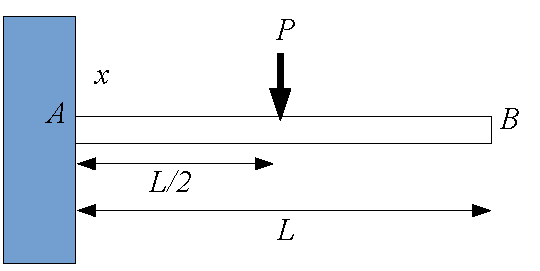
\includegraphics[scale=0.8]{pictures/Static-body-load-analysis/beam-def-midpoint-exercise}
    \caption{Exercise \ref{exercise: beam-deflection-midpoint}}
  \end{figure}
  
  \item Derive the equation of the deflection curve for a simple beam AB loaded by a moment $M_0$ at the left hand support. Also, determine the maximum deflection  (note: use the second order differential equation to determine the deflection $v(x)$, a simple beam is a constant cross sectional beam with Young’s Modulus $E$ and area moment of inertia $I$.)

  \item \label{exercise: beam-deflection-moving-force} What must be the equation $y = f(x)$ of the axis of the slightly curved beam AB before the load is applied in order that the load $P$, moving along the bar, always stays at the same level?

  \begin{figure}[H]
    \centering
    % 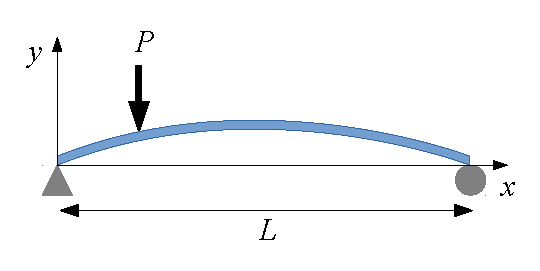
\includegraphics[scale=1]{pictures/Static-body-load-analysis/beam-def-moving-force-exercise}
    \begin{tikzpicture}
      \draw[<->] (0,3) node[left]{$y$} --++ (-90:3) --++ (0:8) node[below]{$x$};
      \draw [line width=6pt, LightSkyBlue] (0,0) node(A){} arc (120:60:7) node[near start](C){} node(B){};
      \draw [<-, ultra thick] (C.center) --++ (90:1) node[above]{$P$};
      \node at (A.center) [anchor=north, regular polygon, regular polygon sides=3, minimum height=4mm, draw, fill=LightGrey, inner sep=0]{};
      \node at (B.center) [anchor=north, circle, minimum height=4mm, draw, fill=LightGrey, inner sep=0]{};
      \draw [|<->|] (A.center) ++ (-90:0.7) --++ (0:7) node[midway, fill=White]{$L$};
    \end{tikzpicture}
    \caption{Exercise \ref{exercise: beam-deflection-moving-force}}
  \end{figure}
  
  \item The cantilever beam shown in the figure supports a triangularly distributed load of maximum intensity $q_0$, determine the deflectionat the free end B. (Obtain the solution by determining the strain energy of the beam and using Castigliano’s theorem)

    \begin{figure}[H]
    \centering
    \begin{tikzpicture}[>=latex]
      \draw[fill=LightGrey] (0,-0.5) rectangle (1,2.5);
      \draw[fill=SkyBlue] (1,0.75) node[above left]{A}  rectangle (7,1.25) node[below right]{B};
      \foreach \x in {0,...,10}
      \draw[<-,thick] (1.0+ 0.6*\x, 1.25) -- ++(90:1.01-\x/10);
      \draw (1,2.25) node[above right]{$q_0$} -- (7,1.25);
      \draw[|<->|] (1, 0.25) -- (4,0.25) node[below]{$L$} --  (7, 0.25);
      \draw (4,1) node{$EI$};
      \draw[->] (1,0.5) -- (1.5,0.5) node[right]{$x$};
    \end{tikzpicture}
  \end{figure}

\item A cat, a mouse, and a tree branch

A 10-N mouse is chased by a 50-N cat onto a \emph{circular} cross-sectioned tree branch ($r$ = 5 mm) which is 10 m long and is 5 cm above ground. The cat is always 5 m behind the mouse. When the mouse gets to the end of the branch, it immediately jumps down to the ground and keeps running away. The branch material properties are $E$ = 10 GPa and $\sigma_{allow}$ = 3 MPa.

\begin{figure}[h]
  \centering
  \begin{tikzpicture}[>=latex]
    \draw (0,0) --++ (-90:0.5) arc (180:270:0.1) node(A){} --++ (0:10) node[midway](B){} node(C){} --++ (-90:0.4) --++ (180:10) arc (90:180:0.1) --++ (-90:1) node(D){};
    \node at (D.center) [anchor=north west, pattern=north west lines, minimum height=5mm, minimum width=10cm](ground1){};
    \draw [|<->|] (D.center) ++ (90:0.8) --++ (0:10) node[midway, fill=White]{10 m};
    \draw [|<->|] (ground1.north east) ++ (0:0.3) --++ (90:1.1) node[midway, right, fill=White]{5 cm};
    \draw (ground1.north west) -- (ground1.north east);
    \node at (A.center) [anchor=south west, draw, minimum height=3mm, minimum width=5mm, fill=DarkGrey](cat1){};
    \draw [<-] (cat1) --++ (90:0.5) node[above]{cat};
    \node at (B.center) [anchor=south, draw, minimum height=3mm, minimum width=2mm, fill=DarkGrey](mouse1){};
    \draw [<-] (mouse1) --++ (90:0.5) node[above]{mouse};
    \node at (D.center) [yshift=-1cm, anchor=west]{Beginning of chase};
    
    \draw (D.center) ++ (-90:2) --++ (-90:0.5) arc (180:270:0.1) node(E){} --++ (0:10) node[midway](F){} node(G){} --++ (-90:0.4) --++ (180:10) arc (90:180:0.1) --++ (-90:1) node(H){};
    \node at (H.center) [anchor=north west, pattern=north west lines, minimum height=3mm, minimum width=10cm](ground2){};
    \draw (ground2.north west) -- (ground2.north east);
    \node at (F.center) [anchor=south west, draw, minimum height=3mm, minimum width=5mm, fill=DarkGrey]{};
    \node at (G.center) [anchor=south, draw, minimum height=3mm, minimum width=2mm, fill=DarkGrey]{};
    \node at (H.center) [yshift=-1cm, anchor=west]{Middle of chase. Mouse about to jump away from branch.};

    \draw (H.center) ++ (-90:2) --++ (-90:0.5) arc (180:270:0.1) node(I){} --++ (0:10) node[midway](J){} node(K){} --++ (-90:0.4) --++ (180:10) arc (90:180:0.1) --++ (-90:1) node(L){};
    \node at (L.center) [anchor=north west, pattern=north west lines, minimum height=3mm, minimum width=10cm](ground3){};
    \draw (ground3.north west) -- (ground3.north east);
    \node at (K.center) [anchor=south, draw, minimum height=3mm, minimum width=5mm, fill=DarkGrey]{};
    \node at (L.center) [yshift=-1cm, anchor=west]{End of chase. Mouse got away. Cat stands at end of branch.};
  \end{tikzpicture}
\end{figure}

Questions:

\begin{enumerate}
\item Does the branch ever touch the ground at any time during the chase? (Show your work.)
\item Does the branch break during the chase? (Again, show your work.)
\end{enumerate}

\begin{pycode}
  L = random.randint(5,12)/10 # 0.5 - 1.2 m
  E = random.randint(5,9)*10*1e9 # 50 - 90 GPa
  sigma_allow = random.randint(10,20)*10*1e6 # 100 - 200 MPa
  frac = random.randint(6,9)/10 # 5/8 - 7/8
  x = frac*L
  delta = random.randint(3,8)*1e-2 # 3 - 8 cm
\end{pycode}

  \item A \py{L}-m long circular cross-sectioned cantilever beam with radius $r$ made of aluminum with $E$ = \py{E/1e9} GPa and $\sigma_{\text{allow}}$ = \py{sigma_allow/1e6} MPa. An upward load $F$ is applied at length \py{round(x,3)} m from the fixed end. Determine the radius $r$ so that the free end of the beam can bend upward at least \py{round(delta/1e-2,2)} cm without failing.

  \begin{figure}[htbp]
    \centering
    \begin{tikzpicture}[>=latex]
      \node[minimum height=1cm, minimum width=5mm, pattern=north west lines](wall){};
      \draw (wall.south east) -- (wall.north east);
      \node at (wall.east) [anchor=west, draw, fill=LightGrey, minimum height=5mm, minimum width=6cm, top color=LightGrey, bottom color=LightGrey, middle color=LightGrey!30](beam){};
      \begin{pycode}
        print(r'\draw [|<->|] (wall.south east) --++ (0:'+str(frac*6)+r') node[midway, below]{'+str(round(x,3))+r' m};')
        print(r'\draw [<-,ultra thick] (beam.south west) ++ (0:'+str(frac*6)+r') --++ (-90:1) node[below]{$P$};')
      \end{pycode}
      \draw [dashed] (beam.east) --++ (0:0.5);
      \draw [->|] (beam.east) ++ (0:0.2) --++ (90:0.5) node[midway, right]{\py{round(delta/1e-2,2)} cm};
    \end{tikzpicture}
  \end{figure}
  
\end{exercises}

%%%%%%%%%%%%%%%%%%%%%%%%%%%%%%%%%%%%%%%%%%%%%%%%%%%%%%%%%%%%%%%%%%%%%%%%%%%%%%%%%%%%%%%%%%%%%%%%%%%%%%%%%%%%%%%%%%%%%%%%%%%%%%%%%%%%%%%%%%%%%%%%%%%%%%%%%%%%%%%%%%%%%%%%%%%%%%

\chapter{Analysis of Multiaxial Stress} \label{chapter: multiaxial stress}

In this section, we will show how to transform the stress components that are associated with a particular coordinate system into ones associated with another coordinate system. Once the transformation equation have been established, we can use them to obtain the maximum normal and shear stress components at a point and find the orientation of the element on which they act.

\section{Plane Stress}

\begin{marginfigure}
  \centering
  \begin{tikzpicture}[>=latex]
    \node [draw, fill=LightBlue, regular polygon, regular polygon sides=4, minimum width=3cm](A){};
    \draw [->,very thick] (A.north) --++ (90:1) node[above]{$\sigma_y$};
    \draw [->,very thick] (A.east) --++ (0:1) node[right]{$\sigma_x$};
    \draw [->,very thick] (A.west) --++ (180:1);
    \draw [->,very thick] (A.south) --++ (-90:1);
    \node at (A.north west) [yshift=3mm] (B){};
    \draw [-left to, very thick] (B) --++ (0:2);
    \node at (A.south east) [xshift=3mm] (C){};
    \draw [-right to, very thick] (C) --++ (90:2) node[above right]{$\tau_{xy}$};
    \node at (A.north west) [xshift=-3mm] (D){};
    \draw [-right to, very thick] (D) --++ (-90:2);
    \node at (A.south east) [yshift=-3mm] (E){};
    \draw [-left to, very thick] (E) --++ (180:2);
    \node at (A.south) [yshift=-1.2cm] {$\sigma_z = 0$, $\tau_{xz} = 0$, $\tau_{yz}  = 0$.};
  \end{tikzpicture}
  % 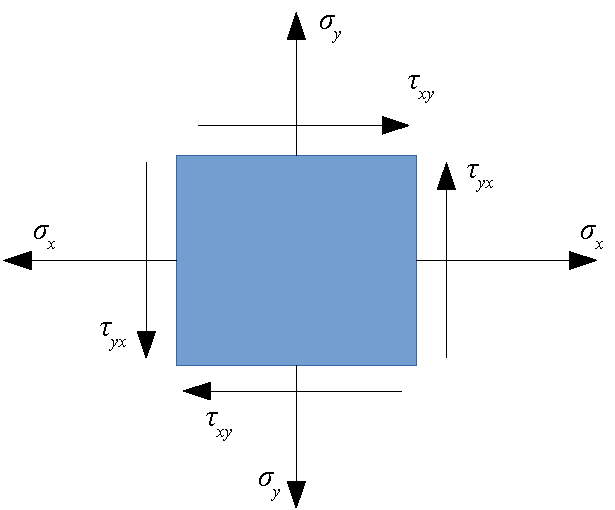
\includegraphics[scale=0.7]{pictures/Multiaxial/plane-stress}
  \caption{A plane stress element.}
  \label{fig: plane stress element}
\end{marginfigure}

Normally, the state of stress at a point in a body is defined by six independent normal and shear stresses. However, this is rarely encountered in real life, as we usually approximate and simplify so that the stress can be analyzed in a single plane. This is called \emph{plane stress}, illustrated in \cref{fig: plane stress element}. In this case, it is assumed that there is no load on the surface of a body and the corresponding stress components (both normal and shear) in the out-of-plane direction are zero. Therefore, the only three components of stress left are $\sigma_x$, $\sigma_y$, and $\tau_{xy}$ which act on the sides of the element.

\section{Stress Transformation for Plane Stress}

The method of transforming the normal and shear stress components from the $x$, $y$ to $x^\prime$, $y^\prime$ coordinate axes will now be developed in a general manner and expressed as a set of stress transformation equations.

\paragraph{Sign Convention:} Before the transformation equations are derived, we must first establish a sign convention for the stress components. A normal or shear stress component is positive when it acts in a positive direction on a positive face, or it acts in a negative direction on a negative face. The stress component is negative otherwise.

Given the state of plane stress, the orientation of the inclined plane on which the normal and shear stress components are to be determined will be defined using $\theta$. Note that both coordinate systems $x$-$y$ and $x^\prime$-$y^\prime$ must form right-handed coordinate systems, meaning the cross product $x \times y$ must give the direction of $z$.

\begin{figure}[h]
  \centering
  \begin{tikzpicture}[>=latex]
    \node [draw, fill=LightBlue, regular polygon, regular polygon sides=4, minimum width=4cm](A){};
    \draw [->,very thick] (A.north) --++ (90:1) node[above]{$\sigma_y$};
    \draw [->,very thick] (A.east) --++ (0:1) node[right]{$\sigma_x$};
    \draw [->,very thick] (A.west) --++ (180:1);
    \draw [->,very thick] (A.south) --++ (-90:1);
    \node at (A.north west) [yshift=3mm] (B){};
    \draw [-left to, very thick] (B) --++ (0:2.6);
    \node at (A.south east) [xshift=3mm] (C){};
    \draw [-right to, very thick] (C) --++ (90:2.6) node[above right]{$\tau_{xy}$};
    \node at (A.north west) [xshift=-3mm] (D){};
    \draw [-right to, very thick] (D) --++ (-90:2.6);
    \node at (A.south east) [yshift=-3mm] (E){};
    \draw [-left to, very thick] (E) --++ (180:2.6);
    \draw [dashed] (A.north west) ++ (-90:0.5) node(F){} ++ (135:1) --++ (-45:6);
    \node at (A.west) [above right]{$\theta$};
    %%%% cut section %%%%
    \draw [fill=LightBlue] (F) ++ (0:8) node(G){} --++ (-90:2.3) node(H){} --++ (0:2.3) node(I){} -- cycle node[midway](J){};
    \draw [->, very thick] (G.center) ++ (-90:1) --++ (180:1) node[above]{$\sigma_x$};
    \draw [->, very thick] (H.center) ++ (0:1.3) --++ (-90:1) node[right]{$\sigma_y$};
    \draw [-left to, very thick] (I.center) ++ (-135:0.5) --++ (180:1.8);
    \draw [-right to, very thick] (G.center) ++ (-135:0.5) --++ (-90:1.8) node[below]{$\tau_{xy}$};
    \draw [->, very thick] (J.center) --++ (45:1) node[above right]{$\sigma_{x^\prime }$};
    \draw [-right to, very thick] (I.center) ++ (90:0.5) --++ (135:2.6) node[above right]{$\tau_{x^\prime y^\prime}$};
  \end{tikzpicture}
  % 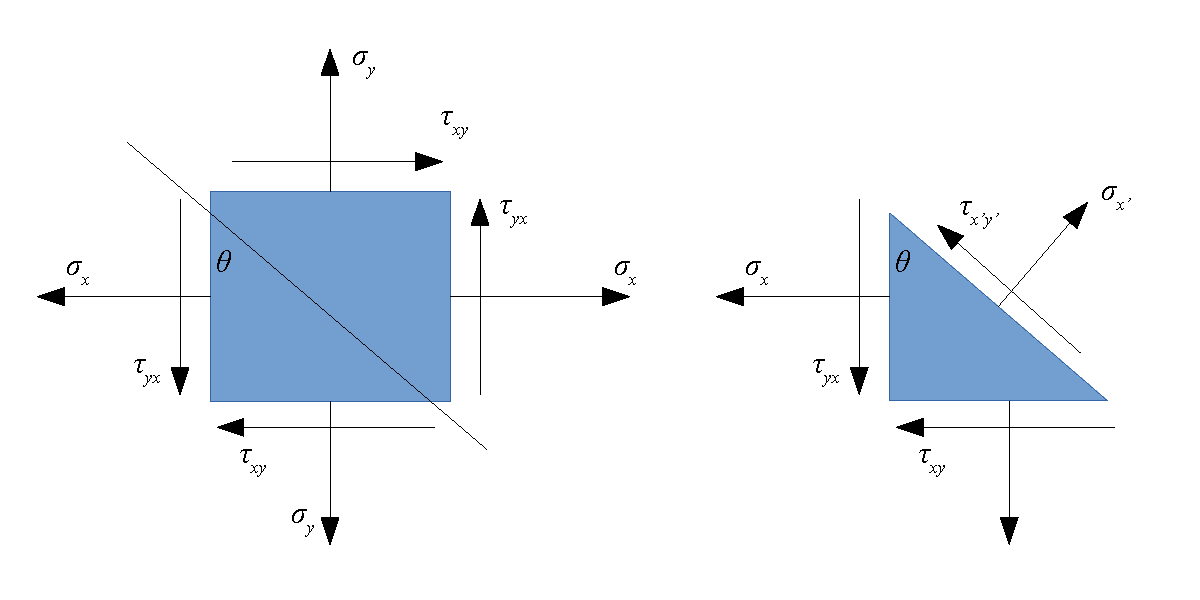
\includegraphics[scale=0.7]{pictures/Static-body-load-analysis/stress-transformation}
  \caption{Derivation of stress transformation equation by cutting element at an angle.}
  \label{fig: stress transformation}
\end{figure}

\paragraph{Normal and Shear Stress Components:} The element is sectioned into a right-angle triangle with an angle of $\theta$ on the top as in the figure below. The resulting normal and shear stress on the newly sectioned side can be determined using equation of force equilibrium as

\begin{gather*}
  \sum F_{x^\prime }  = 0; \hfill \\[1em]
  \begin{split}
    \sigma_{x^\prime }\Delta A - (\tau_{xy}\Delta A\sin \theta )\cos \theta  &- (\sigma _y\Delta A\sin \theta )\sin \theta  \\
    &- (\tau_{xy}\Delta A\cos \theta )\sin \theta  - (\sigma_x\Delta A\sin \theta )\cos \theta  = 0
  \end{split} \nonumber \\[0.5em]
  \sigma_{x^\prime } = \sigma_x\cos ^2\theta  + \sigma_y\sin^2\theta  + 2\tau_{xy} \sin \theta \cos \theta  \\[1em]
  \sum F_{y^\prime}  = 0; \hfill \\ 
  \tau_{x^\prime y^\prime} = -(\sigma_x - \sigma_y)\sin \theta \cos \theta  + \tau_{xy}(\cos ^2\theta  - \sin^2\theta ) \\ 
\end{gather*}

Once we know $\sigma_{x^\prime}, \sigma_{y^\prime}$ can be obtained simply by substituting $\theta$ with 90 + $\theta$

\[\sigma_{y^\prime} = \sigma_x\sin^2\theta  + \sigma_y\cos^2\theta  - 2\tau_{xy}\sin \theta \cos \theta \]

If we know the stress components for all possible orientations of faces through a point, we say that we know the \emph{state of stress} at a point.

\section{Mohr’s Circle for Stress Transformation}

The stress transformation can be made easier to understand through the use of a graphical representation. However, first we have to rewrite stress transformation using double angle formulas.

\begin{align*}
  &\sigma_{x^\prime } = \sigma_x\cos^2\theta  + \sigma_y\sin^2\theta  + 2\tau_{xy}\sin \theta \cos \theta \\
  &\sigma_{x^\prime } = \frac{\sigma_x}{2}(1 + \cos 2\theta ) + \frac{\sigma_y}{2}(1 - \cos 2\theta ) + \tau_{xy}\sin 2\theta \\
  &\sigma_{x^\prime } - \left( \frac{\sigma_x + \sigma_y}{2} \right) = \left( \frac{\sigma_x + \sigma_y}{2} \right)\cos 2\theta  + \tau_{xy}\sin 2\theta 
\end{align*}

\begin{align*}
  &\tau_{x^\prime y^\prime} = (\sigma_y - \sigma_x)\sin \theta \cos \theta  + \tau_{xy}(\cos ^2\theta  - \sin^2\theta ) \\
  &\tau_{x^\prime y^\prime} = \left( \frac{\sigma_y - \sigma_x}{2} \right)\sin 2\theta  + \tau_{xy}\cos 2\theta 
\end{align*}

Square both expressions and add them together, we have

\begin{align*}
  \left[ \sigma_{x^\prime } - \left( \frac{\sigma_x + \sigma_y}{2} \right) \right]^2 + \tau_{x^\prime y^\prime}^2 = &\left( \frac{\sigma_x - \sigma_y}{2} \right)^2\cos^22\theta  + 2\left( \frac{\sigma_x - \sigma_y}{2} \right)\tau_{xy}\cos 2\theta \sin 2\theta  + \tau_{xy}^2{\sin^2}2\theta \\
  + &\left( \frac{\sigma_x - \sigma_y}{2} \right)^2\sin^22\theta  + 2\left( \frac{\sigma_y - \sigma_x}{2} \right)\tau_{xy}\cos 2\theta \sin 2\theta  + \tau_{xy}^2\cos^22\theta
\end{align*}

Simplifying the expression using trigonometry identities, we have

\[\left[ \sigma_{x^\prime } - \left( \frac{\sigma_x + \sigma_y}{2} \right) \right]^2 + \tau_{x^\prime y^\prime}^2 = \left( \frac{\sigma_x - \sigma_y}{2} \right)^2 + \tau _{xy}^2\]

Since $\sigma_x$, $\sigma_y$, and $\tau_{xy}$ are known quantities for the problem, we can rewrite the expression as

\begin{equation}
  (\sigma_{x^\prime } - \sigma_{avg})^2 + \tau_{x^\prime y^\prime}^2 = R^2
\end{equation}

Note that this equation represents a circle having radius $R$ and center on the $\sigma$ axis at point ($\sigma_{avg}$, 0).

\begin{figure}[h]
  \centering
  \begin{tikzpicture}
    \node at (-3,0) [anchor=west, draw, fill=SkyBlue, circle, minimum height=7cm](large){};
    \draw [<->] (-5,0) --++ (0:10) node[right]{$\sigma$};
    \draw [<->] (0,-5) --++ (90:10) node[above]{$\tau$};
    \node at (large.east) [below right] {$\sigma_1$};
    \node at (large.west) [below left] {$\sigma_2$};
    \draw (0,0) node[below left]{0};
    \draw [dashed](large.center) -- (large.south) node[below right](absolute){$(\tau_{x^\prime y^\prime})_{\max}$};
    \draw (large.center) --++ (50:3.5) node[above right]{$\sigma_x$} node(A){};
    \draw (large.center) --++ (-130:3.5) node[below left]{$\sigma_y$};
    \draw [dashed] (A.center) --++ (180:2.75) node[left]{$\tau_{xy}$};
    \draw (absolute.south) [out=-90, in=150] to ++(0.5,-0.5) node[right]{Maximum in-plane shear stress};
  \end{tikzpicture}
  \caption{Mohr's circle and its representation of state of stress.}
  \label{fig: mohr's circle}
\end{figure}

This extremely useful graphical representation for stress transformation was developed by a German engineer Otto Mohr and is therefore called \emph{Mohr’s circle}.
The original state of stress can be determined by

\begin{equation} \label{eqn: principal direction}
  2\theta_p = \tan^{-1}\frac{2\tau_{xy}}{\sigma_x - \sigma_y}
\end{equation}

where $\theta _p$ is called the \emph{principal direction}. And when determining the stress components in the material at angle $\alpha$ from its original coordinate system, simply draw the line from the center of the circle at angle $2\alpha$ from the original state to determine stress components at this new orientation.

\subsection{Principal Stresses for Plane Stress}

Considering the two points where the circle crosses the $\sigma$ axis, these two points are where the two normal stress components are at maximum and minimum. These two stresses are called the maximum and minimum principal stresses, respectively. We can represent them in terms of stresses in plane stress as

\begin{equation} \label{eqn: principal stresses}
  \sigma_{1,2} = \frac{\sigma_x + \sigma_y}{2} \pm \sqrt {\frac{\sigma_x - \sigma_y}{2}^2 + \tau _{xy}^2}
\end{equation}

Also note that the shear stress component is zero in this orientation.

\subsection{Maximum In-Plane Shear Stresses}

At the highest point of the circle represents the maximum shear stress and its orientation. We can represent the maximum shear stress in terms of stresses in plane stress as

\begin{equation} \label{eqn: max shear stress}
  \tau_{xy} = \sqrt {\left( \frac{\sigma_x - \sigma_y}{2} \right)^2 + \tau_{xy}^2}
\end{equation}

Since the angle between the principal stresses and maximum shear stress on Mohr’s circle is 90 degree, the actual angle between the principal stress plane and maximum shear stress plan is 45. Also note that the normal component stresses are equal to $\sigma_{avg}$.

\begin{example} State of stress of a plane stress element \label{example: plane stress}
  
  Determine the principal stresses, maximum shear stress, and the principal direction in this element 

  \begin{figure}[H]
    \centering
    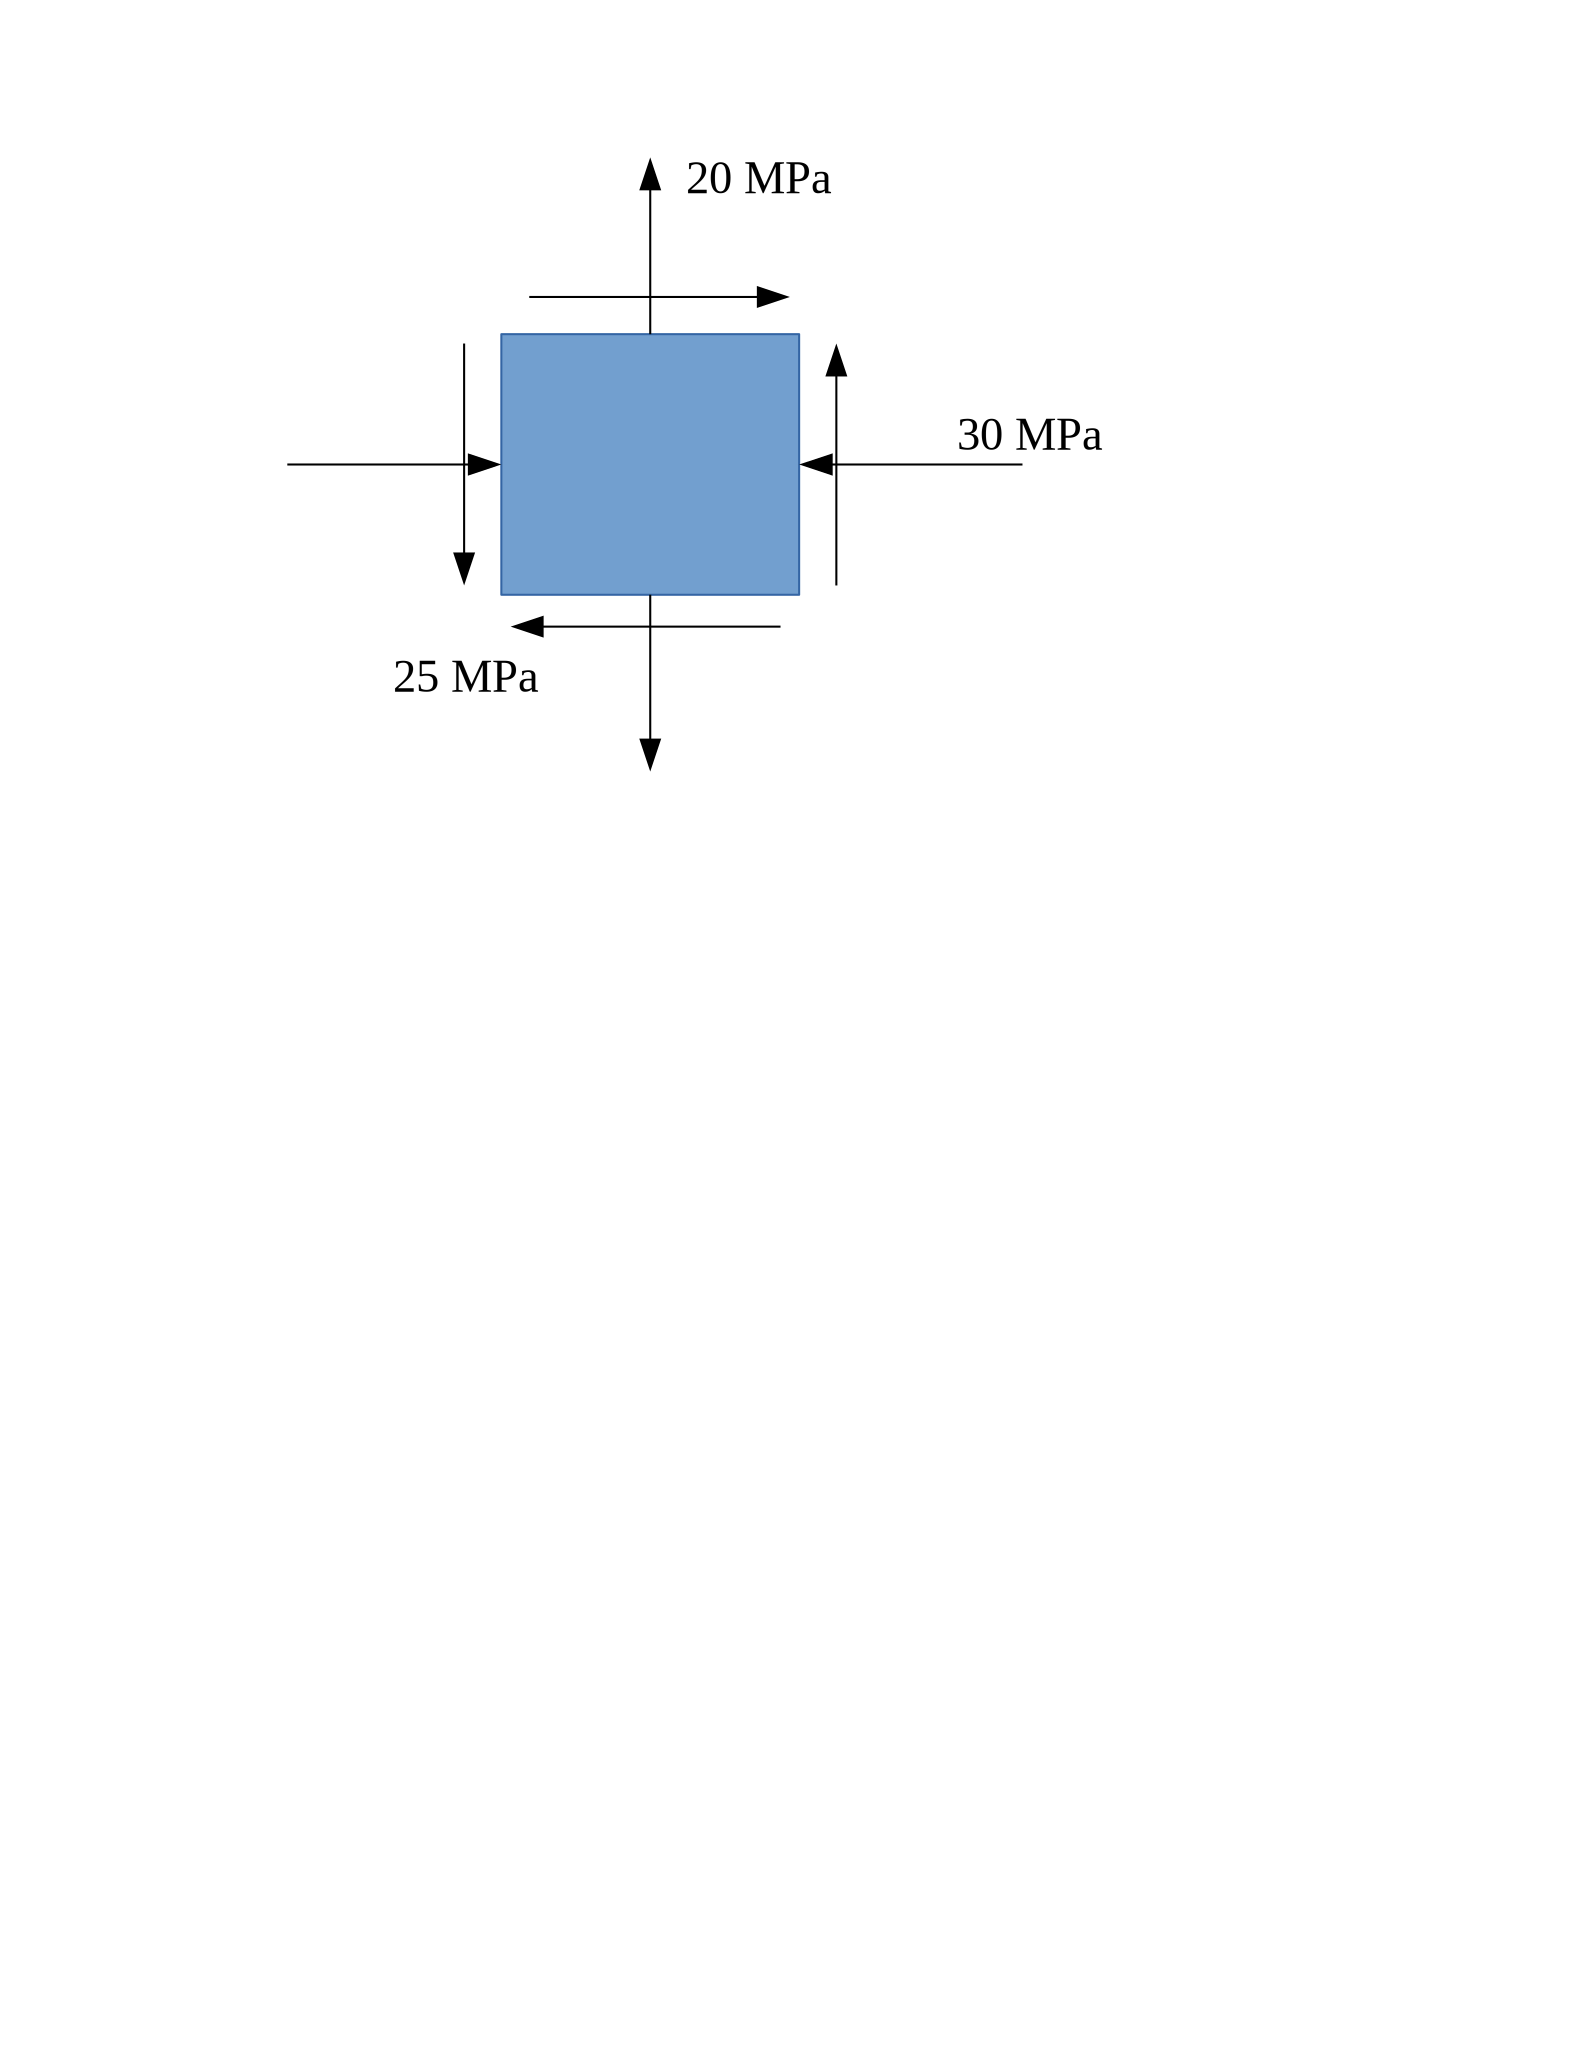
\includegraphics[scale=0.5]{pictures/Static-body-load-analysis/plane-stress-example}
    \caption{\Cref{example: plane stress}}
  \end{figure}
\end{example}
\begin{solution}
  To determine the maximum shear stress, simply substitute the values into \cref{eqn: max shear stress} and obtain
  
  \begin{align*}
    \tau_{xy} &= \sqrt {\left( \frac{\sigma_x - \sigma_y}{2} \right)^2 + \tau _{xy}^2}  \\ 
                 &= \sqrt {\left( \frac{-30 - 20)}{2} \right)^2 + 25^2}  \\ 
                 &= 35.4 \text{ MPa} 
  \end{align*}
  
  The principal stresses are

  \begin{align*}
    \sigma_{1,2} &= \frac{\sigma_x + \sigma _y}{2} \pm \sqrt {\frac{\sigma _x - \sigma_y}{2}^2 + \tau _{xy}^2}  \\ 
                    &= \frac{-30 + 20}{2} \pm 35.4 \\ 
                    &= 30.4 \text{ MPa}, - 40.4 \text{ MPa} 
  \end{align*}
  
  The principal direction is

  \begin{align*}
    2\theta  &= \tan^{-1}\frac{2\tau_{xy}}{\sigma_x - \sigma_y} \\ 
             &= \tan^{-1} -1 \\ 
             &= -45\degree \\
    \theta  &= -22.5\degree
  \end{align*}

  We can also plot the expression for transformed normal stress $\sigma_x^\prime $ and transformed shear stress $\tau_{x^\prime y^\prime}$ as

  \begin{figure}[H]
    \centering
    \begin{tikzpicture}
      \begin{axis} [
        width=0.8\textwidth,
        height=0.5\textwidth,
        samples=50,
        xlabel={$\theta$},
        ylabel={Stress (MPa)},
        domain=0:360,
        xtick distance=45,
        xmin=0,
        ]
        \addplot+[mark=none]{-30*(cos(x))^2 + 20*(sin(x))^2 + 50*sin(x)*cos(x)} node[right]{$\sigma_x^\prime $};
        \addplot+[mark=none]{-(-30 - 20)*sin(x)*cos(x) + 25*((cos(x))^2 - (sin(x))^2)} node[right]{$\tau_{x^\prime y^\prime}$};
      \end{axis}
    \end{tikzpicture}
  \end{figure}

  where we can observe that the principal direction and max shear stress direction are always 45$^{\circ}$ apart.

  Finally, to bring things full circle (literally), let us draw a Mohr's circle to represent the state of stress.

  \begin{figure}[H]
    \centering
    \begin{tikzpicture}
      \node at (-4,0) [anchor=west, draw, fill=SkyBlue, circle, minimum height=7cm](large){};
      \draw [<->] (-5,0) --++ (0:9) node[right]{$\sigma$};
      \draw [<->] (0,-4.5) --++ (90:9) node[above]{$\tau$};
      \node at (large.east) [below right] {30.4};
      \node at (large.west) [below left] {-40.4};
      \draw (0,0) node[below right]{0};
      \draw (large.south west) -- (large.north east);
      \draw [dashed] (large.north east) --++ (-90:2.5) node[below]{20};
      \draw [dashed] (large.south west) --++ (0:3) node[right]{25};
      \draw [dashed] (large.south west) --++ (90:2.45) node[above]{-30};
      \node at (0,0) [above right]{-45$^{\circ}$};
      \draw [-latex] (large.center) ++ (45:1.5) arc (45:0:1.5);
    \end{tikzpicture}
  \end{figure}
\end{solution}

\section{Hooke’s Law for Plane Stress}

We have previously investigated the stresses in a plane-stress element. We will now use them in combination with Hooke’s law to derive the strains in the material. Here, we will have to assume that the material is uniform throughout the body and has the same properties in all directions.

Consider the normal strains $\varepsilon_x$, $\varepsilon_y$, and $\varepsilon_z$ in plane stress. Each strain is the summation of effects of individual stresses. For example, the strain $\varepsilon_x$ due to the stress $\sigma_x$ is $\sigma_x / E$ where $E$ is the modulus of elasticity. Also, the strain $\varepsilon_x$ due to the stress $\sigma_y$ is equal to $-\nu \sigma_y / E$ where $\nu$ is the Poisson’s ratio. Since there is no stress in the $z$ direction and the shear stresses produce no normal strains, we have the resultant strain in the x direction is

\begin{equation} \label{eqn: plane stress x}
  \varepsilon_x = \frac{1}{E}(\sigma_x - \nu \sigma_y)
\end{equation}

And in a similar manner, we obtain the strains in the $y$ and $z$ directions as:

\begin{align} \label{eqn: plane stress y and z}
  \varepsilon_y &= \frac{1}{E}(\sigma_y - \nu \sigma_x) \nonumber \\
  \varepsilon_z &=  - \frac{\nu }{E}(\sigma_x + \sigma_y)
\end{align}

These equations may be used to find the normal strains when the stresses are known.

The shear stress causes a distortion of the element. The shear strain $\tau_{xy}$ is the decrease in angle between the $x$ and $y$ faces of the element and is related to the shear stress by Hooke’s law in shear as follows:

\begin{equation}
  \gamma_{xy} = \frac{\tau_{xy}}{G}
\end{equation}

where $G$ is the shear modulus of elasticity. Note that the normal stresses have no effect on the shear strain.

\Cref{eqn: plane stress x} and \cref{eqn: plane stress y and z} can be solved simultaneously for the stresses in terms of the strains, so we have:
\begin{equation}
  \begin{gathered}
    \sigma_x = \frac{E}{1 - \nu^2}(\varepsilon_x + \nu \varepsilon_y) \hfill \\
    \sigma_y = \frac{E}{1 - \nu^2}(\varepsilon_y + \nu \varepsilon_x) \hfill \\ 
  \end{gathered}
\end{equation}

These equations may be used to find the stresses in plane stress when the strains are known.

\subsection{Special cases of Hooke’s law}

In the special case of biaxial stress, we only have normal stresses in the $x$ and $y$ directions. There is no normal stress in the out-of-plane direction and there is no shear stress at all. In this case, Hooke’s law for plane stress simplifies to
\begin{equation}
  \begin{gathered}
    \varepsilon_x = \frac{1}{E}(\sigma_x - \nu \sigma_y) \hfill \\
    \varepsilon_y = \frac{1}{E}(\sigma_y - \nu \sigma_x) \hfill \\
    \varepsilon_z =  - \frac{\nu }{E}(\sigma_x + \sigma_y) \hfill \\ 
  \end{gathered}
\end{equation}

And the corresponding normal stresses are:

\begin{equation}
  \begin{gathered}
    \sigma_x = \frac{E}{1 - \nu^2}(\varepsilon_x + \nu \varepsilon_y) \hfill \\
    \sigma_y = \frac{E}{1 - \nu^2}(\varepsilon_y + \nu \varepsilon_x) \hfill
  \end{gathered}
\end{equation}

For uniaxial stress, there is only a normal stress in the $x$ direction, the equations of Hooke’s law simplify further to:

\begin{equation}
  \begin{gathered}
    \varepsilon_x = \frac{1}{E}({\sigma _x} - \nu \sigma_y) \hfill \\
    \varepsilon_y = {\varepsilon _z} =  - \frac{\nu }{E}{\sigma _x} \hfill \\ 
  \end{gathered}
\end{equation}

\subsection{Unit volume change}

The unit volume change at a point in a strained body can be found by considering the deformed element. Assume that the original volume of this element is $V_0 = abc$, its final volume is

\[V_1 = abc(1 + \varepsilon_x)(1 + \varepsilon_y)(1 + \varepsilon_z)\]

Expanding the expression, we have

\[V_1 = abc(1 + \varepsilon _x + \varepsilon _y + \varepsilon _z + \varepsilon_x\varepsilon_y + \varepsilon_x\varepsilon_z + \varepsilon_y\varepsilon_z + \varepsilon_x\varepsilon_y\varepsilon_z)\]

Since we assume that the strains are very small, we can ignore the products of the small strains and the final volume becomes

\[V_1 = abc(1 + \varepsilon_x + \varepsilon_y + \varepsilon_z)\]

Therefore, the change in volume is

\[\Delta V = V_1 - V_0 = abc(\varepsilon_x + \varepsilon_y + \varepsilon_z)\]

And the unit volume change, or dilatation, becomes

\begin{equation} \label{eqn: 2d dilatation}
  e = \frac{\Delta V}{V_0} = \varepsilon_x + \varepsilon_y + \varepsilon_z
\end{equation}

This equation gives the dilatation in terms of the normal strains and is valid for any material provided the strains are small. Observe once again that shear strains produce no change in volume. When the material follows Hooke’s law, we can substitute equations 6140 and 6141 into equation 6151 and obtain the following expression for the unit volume change in plane stress in terms of the stresses:

\begin{equation}
  e = \frac{\Delta V}{V_0} = \frac{1 - 2\nu}{E}(\sigma_x + \sigma_y)
\end{equation}
  
Having this expression for $e$, we can find the volume change for any object subjected to plane stress by integrating throughout its volume.

\section{Triaxial Stress}

When an element of material is subjected to normal stresses in all three perpendicular directions and there are no shear stresses in the faces, the element is said to be in a state of triaxial stress. Since there are no shear stresses, the three normal stresses are the principal stresses in the material.

From our previous discussion of plane stresses, we know that the maximum shear stresses occur on planes oriented at 45 degree to the principal plane. Therefore, for a material in triaxial stress, the maximum shear stresses occur on elements oriented at angles of 45 degree to the $x$, $y$, and $z$ axes. Therefore, the maximum shear stresses obtained by the rotation about the axes are

\begin{equation}
  \begin{gathered}
    (\tau_{\max })_z =  \pm \frac{\sigma_x - \sigma_y}{2} \hfill \\
    (\tau_{\max })_x =  \pm \frac{\sigma_y - \sigma_z}{2} \hfill \\
    (\tau_{\max })_y =  \pm \frac{\sigma_x - \sigma_z}{2} \hfill \\ 
  \end{gathered}
\end{equation}

The absolute maximum shear stress is the numerically the largest of the stresses from equation 6153.

\subsection{Hooke’s law for triaxial stress}

If the material follows Hooke’s law, we can obtain the relationships between the normal stresses and normal strains by using the same procedure as for plane stress. The strains produced by the stresses $\sigma_x$, $\sigma_y$, and $\sigma_z$ acting independently are superimposed to obtain the resultant strains. We can then derive the equations for strains in triaxial stress as follow:

\begin{equation}
  \begin{gathered}
    \varepsilon_x = \frac{\sigma_x}{E} - \frac{\nu }{E}(\sigma_y + \sigma_z) \hfill \\
    \varepsilon_y = \frac{\sigma_y}{E} - \frac{\nu }{E}(\sigma_x + \sigma_z) \hfill \\
    \varepsilon_z = \frac{\sigma_z}{E} - \frac{\nu }{E}(\sigma_x + \sigma_y) \hfill 
  \end{gathered}
\end{equation}

These equations can then be solved simultaneously for the stresses in terms of the strains.

\begin{equation}
  \begin{gathered}
    \sigma_x = \frac{E}{(1 + \nu )(1 - 2\nu )}\left[ (1 - \nu )\varepsilon_x + \nu (\varepsilon_y + \varepsilon_z) \right] \hfill \\
    \sigma_y = \frac{E}{(1 + \nu )(1 - 2\nu )}\left[ (1 - \nu )\varepsilon_y + \nu (\varepsilon_x + \varepsilon_z) \right] \hfill \\
    \sigma_z = \frac{E}{(1 + \nu )(1 - 2\nu )}\left[ (1 - \nu )\varepsilon_z + \nu (\varepsilon_x + \varepsilon_y) \right] \hfill \\ 
  \end{gathered}
\end{equation}

These equations are also known as \emph{Hooke’s law for triaxial stress}.

\subsection{Unit Volume Change}

From \cref{eqn: 2d dilatation} the unit volume change is simply the sum of the normal stresses so that

\begin{equation}
  e = \frac{\Delta V}{V_0} = \varepsilon_x + \varepsilon_y + \varepsilon _z
\end{equation}

In triaxial stress, since all three normal stresses exist without any shear stress, the unit volume change corresponding to those stress are

\begin{equation}
  e = \frac{1 - 2\nu}{E}(\sigma_x + \sigma_y + \sigma_z)
\end{equation}

\subsection{Spherical stress}

In a special case of triaxial stress where all three perpendicular stresses are of the same magnitude, the material is said to be under \emph{spherical stress} or \emph{hydrostatic stress}. In this case, the stresses can be written as

\[\sigma_x = \sigma_y = \sigma_z = \sigma_o\]

Intuitively, the normal strains are also equal.

\[\varepsilon _x = \varepsilon _y = \varepsilon _z = \varepsilon _o = \frac{\sigma _o}{E}(1 - 2\nu )\]

The unit volume change or dilatation under spherical stress is

\begin{equation}
  e = 3\varepsilon_o = \frac{3\sigma_o}{E}(1 - 2\nu )
\end{equation}

The constant of the ratio between the spherical stress and unit volume change is

\begin{equation}
  K = \frac{E}{3(1 - 2\nu )}
\end{equation}

where $K$ is called the \emph{volume modulus of elasticity} or \emph{bulk modulus}.

\begin{example}
A 0.25-m$^3$ cube is being submerged under water where the water pressure is 30 MPa. If the material has $E$ = 3 GPa and Poisson’s ratio of 0.3, find the final volume of the element.
\end{example}
\begin{solution}
Hydrostatic pressure situation represents the state where the pressure is equal in all direction, this means that we can assume that the element is under spherical stress. The unit volume change is

\begin{align*}
  e &= \frac{3\sigma_o}{E}(1 - 2\nu ) \\ 
    &= \frac{3(-30 \times 10^6 \text{ Pa})(1 - 2(0.3))}{(3 \times 10^9 \text{ Pa})} \\ 
    &= -0.012 
\end{align*}	

This means that the volume reduced by 1.2\% (since hydrostatic pressure in this case is compressive), and thus the final volume is

\begin{align*}
  V_f &= (1 + e)V \\ 
      &= 0.988(0.25 \text{ m}^3) \\ 
      &= 0.247 \text{ m}^3
\end{align*}

\end{solution}

\subsection{Absolute Maximum Shear Stress}

In any three-dimensional element, we can determine the 3 principal stresses so that the element is in an equivalent trixial stress state. Though the method of determining three dimensional principal stresses are beyond the scope of this material, we can make simplifying assumptions using plane stress to understand its concept.

Consider a material subjected to in-plane principal stresses $\sigma_1$ and $\sigma_2$. If we look at the element in two dimensions, then we can use Mohr's circle to determine the maximum in-plane shear stress for each of the planes $x$-$y$, $x$-$z$, and $y$-$z$. We can furthermore determine the \emph{absolute maximum shear stress} in the material, which is equal to half of the biggest difference among the three principal stresses. In other words, for a plane stress element where $\sigma_1 > \sigma_2$, we have that

\begin{figure}[h]
  \centering
  \begin{tikzpicture}
    \draw [<->] (0,-5) --++ (90:10) node[above]{$\tau$};
    \node at (0,0) [anchor=west, draw, fill=SkyBlue, circle, minimum height=7cm](large){};
    \node at (0,0) [anchor=west, draw, fill=SkyBlue!50, circle, minimum height=3cm](left){};
    \node at (left.east) [anchor=west, draw, fill=SkyBlue!50, circle, minimum height=4cm](right){};
    \draw [<->] (-2,0) --++ (0:10) node[right]{$\sigma$};
    \node at (large.east) [below right] {$\sigma_1$};
    \node at (large.west) [below left] {0};
    \draw (right.west) [out=70, in=180] to ++(0.5,0.5) node[right]{$\sigma_2$};
    \draw (left.center) -- (left.south) node[below]{$(\tau_{y^\prime z^\prime})_{\max}$};
    \draw (right.center) -- (right.south) node[below](inplane){$(\tau_{x^\prime y^\prime})_{\max}$};
    \draw (inplane.south) [out=-80, in=150] to ++(0.5,-0.5) node[right]{Maximum in-plane shear stress};
    \draw (large.center) -- (large.south) node[below](absolute){$(\tau_{x^\prime z'})_{\max}$};
    \draw (absolute.south) [out=-90, in=90] to ++(-0.5,-0.5) node[below]{Absolute maximum shear stress};
  \end{tikzpicture}
  \caption{Mohr's circles of a plane stress element in each of the planes $x$-$y$, $x$-$z$, and $y$-$z$ when the stresses are positive.}
\end{figure}

\begin{figure}[h]
  \centering
  \begin{tikzpicture}
    \node at (-3,0) [anchor=west, draw, fill=SkyBlue, circle, minimum height=7cm](large){};
    \node at (0,0) [anchor=east, draw, fill=SkyBlue!50, circle, minimum height=3cm](left){};
    \node at (0,0) [anchor=west, draw, fill=SkyBlue!50, circle, minimum height=4cm](right){};
    \draw [<->] (-5,0) --++ (0:10) node[right]{$\sigma$};
    \draw [<->] (0,-5) --++ (90:10) node[above]{$\tau$};
    \node at (large.east) [below right] {$\sigma_1$};
    \node at (large.west) [below left] {$\sigma_2$};
    \draw (right.west) [out=70, in=180] to ++(0.5,0.5) node[right]{0};
    \draw (left.center) -- (left.south) node[below]{$(\tau_{y^\prime z^\prime})_{\max}$};
    \draw (right.center) -- (right.south) node[below](inplane){$(\tau_{x^\prime y^\prime})_{\max}$};
    \draw (inplane.south) [out=-80, in=150] to ++(0.5,-0.5) node[right]{Maximum in-plane shear stress};
    \draw (large.center) -- (large.south) node[below](absolute){$(\tau_{x^\prime z^\prime})_{\max}$};
    \draw (absolute.south) [out=-90, in=150] to ++(0.5,-0.5) node[right]{Absolute maximum shear stress};
  \end{tikzpicture}
  \caption{Mohr's circles of a plane stress element in each of the planes $x$-$y$, $x$-$z$, and $y$-$z$ when the stresses are of different signs.}
\end{figure}

\begin{equation}
  \tau_{max,abs} = \left\{
    \begin{gathered}
      \dfrac{\sigma_1}{2} \hspace{1.5cm} \text{when } \dfrac{\sigma_1}{\sigma_2} > 0 \\[10pt]
      \dfrac{\sigma_1 - \sigma_2}{2} \hfill \text{when } \dfrac{\sigma_1}{\sigma_2} < 0
    \end{gathered}
  \right.
\end{equation}

Calculating this absolute maximum shear stress as shown here will be crucial when designing components from a ductile material, since its strength mainly depends on its ability to resist shear stress. A more detailed discussion of ductile material strength and failure takes place in \cref{section: yield and fracture}.

\section{** Plane Strain **}

A general state of strain can, just like a state of stress, be represented by a combination of three component of normal strains and three shear strains, $\varepsilon_x$, $\varepsilon_y$, $\varepsilon_z$, $\gamma_{xy}$, $\gamma_{xz}$, and $\gamma_{yz}$. Also strains, like stresses, vary according to the orientation of the element. Strains at a point are often determined using strain gages, which measure strain in specified directions. However, we sometimes need to obtain strain in other directions. That is where \emph{strain transformation} comes in.

Three dimensional strain transformation is beyond the scope of this material. In our case, we will simplify the process for a \emph{plane strain} element. Similar to its plane stress counterpart, a plane strain element has no normal strain in the $z$ direction and no out-of-plane shear strains $\gamma_{xz}$ and $\gamma_{yz}$.

\begin{figure}[h]
  \centering
  \begin{tikzpicture}[>=latex]
    \draw [fill=LightBlue!50] (0,0) node(mid){} --++ (30:1.5) node(ne){}--++ (150:1.5) node(n){} --++ (-150:1.5) node(nw){} -- (mid.center);
    \draw [fill=LightBlue!10!SkyBlue] (mid.center) --++ (-90:1.5) node(s){} --++ (30:1.5) node(se){} -- (ne.center) -- cycle;
    \draw [fill=LightBlue!90!SkyBlue] (mid.center) -- (s.center) --++ (150:1.5) node(sw){} -- (nw.center) -- cycle;
    \draw (se) --++ (-30:2) node[below right]{$y$};
    \draw (sw) --++ (-150:2) node[below left]{$x$};
    \draw (n) --++ (90:2) node[above]{$z$};
    \draw [->, thick] (sw) ++ (90:0.5) ++ (-30:0.75) --++ (-150:1.5) node[below right]{$\sigma_x$};
    \draw [->, thick] (se) ++ (90:0.5) ++ (-150:0.75) --++ (-30:1.5) node[below left]{$\sigma_y$};
    \draw [->, thick] (se) ++ (90:0.5) ++ (150:0.75) ++ (30:0.75) --++ (30:0.75);
    \draw [->, thick] (sw) ++ (90:0.5) ++ (30:0.75) ++ (150:0.75) --++ (150:0.75);
    \draw [dashed] (sw) ++ (-150:0.3) --++ (-30:1.8);
    \draw [dashed] (se) ++ (-30:0.3) --++ (-150:1.8);
    \draw [dashed] (sw) ++ (-150:0.3) --++ (90:1.5) node(w){} --++ (-30:1.8) --++ (-90:1.5);
    \draw [dashed] (se) ++ (-30:0.3) --++ (90:1.5) node(e){} --++ (-150:1.8);
    \draw [dashed] (w.center) --++ (30:0.3) --++ (-30:1.5);
    \draw [dashed] (e.center) --++ (150:0.3) --++ (-150:1.5);
    \draw (w.north) --++ (90:0.3);
    \draw (nw.north) --++ (90:0.3) node[midway](midleft){};
    \draw [->] (midleft.center) --++ (-150:0.3) node[midway, above, yshift=2mm]{$\varepsilon_x dx$};
    \draw (e.north) --++ (90:0.3);
    \draw (ne.north) --++ (90:0.3) node[midway](midright){};
    \draw [->] (midright.center) --++ (-30:0.3) node[midway, above, yshift=2mm]{$\varepsilon_y dy$};
  \end{tikzpicture}
  \caption{Three-dimensional plane strain  element.}
\end{figure}

It is important to realize that plane stress does not cause plane strain or vice versa.

\subsection{Plane-Strain Transformation}

It is important in plane-strain analysis to establish equations to determine the $x^\prime $, $y^\prime$, and shear strain in the $x^\prime y^\prime$ plane at a point when the $x$, $y$ components of strain are known. Unlike plane-stress transformation that can be solved by equilibrium, this is a geometry-based problem, requiring us to show how the changes in lengths of the element vary according to its orientation.

To develop the strain transformation equation for $\varepsilon_{x^\prime }$, we must determine the elongation of a line segment $dx^\prime $ that lies aong th e$x^\prime $ axis and is subjected to strain components $\varepsilon_x$, $\varepsilon_y$, and $\gamma_{xy}$. As illustrated in figure \cref{fig: plane strain before deformation}, the components of the line $dx^\prime $ along the $x$ and $y$ axes are

\begin{figure}[h]
  \centering
  \begin{tikzpicture}[>=latex]
    \draw [thick, DeepSkyBlue] (0,0) node(O){} --++ (0:4) node[midway, below, black]{$dx$} node(A){};
    \draw [thick, DeepSkyBlue] (O.center) --++ (90:2) node[midway, right, black]{$dy$} node(B){};
    \draw [thick, DeepSkyBlue] (O.center) -- (4,2) node[midway, below, black]{$dx^\prime $} node(C){};
    \draw [dashed] (B.center) -- (C.center) -- (A.center);
    \draw (A) --++ (0:1) node[right]{$x$};
    \draw (B) --++ (90:1) node[above]{$y$};
    \draw (O.center) --++ (110:3) node[above]{$y^\prime$};
    \draw (C) --++ (1,0.5) node[above right]{$x^\prime $};
    \draw [->] (4.7,0) arc (0:26.8:4.7) node[midway, right]{$\theta$};
  \end{tikzpicture}
  \caption{Dimensions of plane strain element before deformation.}
  \label{fig: plane strain before deformation}
\end{figure}

\begin{align*}
  dx &= dx^\prime  \cos \theta \\
  dy &= dx^\prime  \sin \theta
\end{align*}

When there is a positive normal strain $\varepsilon_x$ on the material, the line $dx$ is elongated by $\varepsilon_x dx$, which causes $dx^\prime $ to elongate by $\varepsilon_x dx \cos \theta$. Similarly, when $\varepsilon_y$ occurs, line $dy$ elongates by $\varepsilon_y dy$, causing $dy^\prime$ to elongates by $\varepsilon_y dy \sin \theta$. Finally, if we assume that $dx$ is fied, the shear strain $\gamma_{xy}$, which is the change in angle between $dx$ and $dy$, causes the top of line $dy$ to move by $\gamma_{xy} dy$ to the right. This causes $dx^\prime $ to elongate by $\gamma_{xy} dy \cos \theta$. If all three of these elongations are added togather, the resultant elongation of $dx^\prime $, which we will call $\delta x^\prime $, is

\begin{figure}[h]
  \centering
  \begin{tikzpicture}[>=latex]
    \draw [thick, DeepSkyBlue] (0,0) node(O){} --++ (0:4) node[midway, below, black]{$dx$} node(A){};
    \draw [thick, DeepSkyBlue] (O.center) --++ (90:2) node[midway, right, black]{$dy$} node(B){};
    \draw [thick, DeepSkyBlue] (O.center) -- (4,2) node[midway, below, black]{$dx^\prime $} node(C){};
    \draw [->, thick, DeepSkyBlue] (A) --++ (0:1.68) node[midway, below, black]{$\varepsilon_x dx$} node(E){};
    \draw (E) --++ (0:1) node[right]{$x$};
    \draw [->, thick, DeepSkyBlue] (A.east) --++ (26.5:1.5) node[midway](G){} node(F){}; 
    \draw (G.center) to [out=80, in=180] ++(1,1.5) node[right]{$\varepsilon_x dx \cos \theta$};
    \draw [->, thick, DeepSkyBlue] (F.center) -- (E.center) node[midway](H){};
    \draw (H.center) to [out=30, in=90] ++(0.5,-1) node[below]{$\varepsilon_x dx \sin \theta$};
    \draw (F) --++ (26.5:1);
    \draw [->] (E) ++ (0:0.5) arc (0:26.6:2) node[midway, right]{$\theta$};
    \draw (B) --++ (90:1) node[above]{$y$};
    \draw (O.center) --++ (110:3) node[above]{$y^\prime$};
    \draw [->, thick, DeepSkyBlue] (C) --++ (1.5,0.75) node(D){};
    \draw (D) --++ (1,0.5) node[above right]{$x^\prime $};
    \draw [dashed] (A.east) --++ (90:2);
    \draw [dashed] (D.center) --++ (-90:2.8);
  \end{tikzpicture}
  \caption{Plane strain element under normal strain $\varepsilon_x$}
\end{figure}

\begin{figure}[h]
  \centering
  \begin{tikzpicture}[>=latex]
    \draw [thick] (0,0) node(O){} --++ (0:4) node[midway, below, black]{$dx$} node(A){} node[right]{$x$};
    \draw [thick, DeepSkyBlue] (O.center) --++ (90:2) node[midway, right, black]{$dy$} node(B){};
    \draw [thick, DeepSkyBlue] (O.center) -- (4,2) node[midway, below, black]{$dx^\prime $} node(C){};
    \draw [->, thick, DeepSkyBlue] (B) --++ (90:3.2) node[at start](F){} node(G){} node[midway, left, black]{$\varepsilon_y dy$};
    \draw (G) --++ (90:1) node[above]{$y$};
    \draw [->, thick, DeepSkyBlue](F.center) --++ (26.5:1.35) node(H){} node[midway, right, black]{$\varepsilon_y dy \sin \theta$};
    \draw [->, thick, DeepSkyBlue] (H.center) --++ (116.5:2.75) node[midway, right, black]{$\varepsilon_y dy \cos \theta$};
    \draw (H) --++ (26.5:1.5) node[near end](I){};
    \draw [<->] (I.center) arc (26.5:0:1.2) node[midway, right]{$\theta$};
    \draw (O.center) --++ (110:3) node[above]{$y^\prime$};
    \draw [->, thick, DeepSkyBlue] (C) --++ (1.5,0.75) node(D){};
    \draw (D) --++ (1,0.5) node[above right]{$x^\prime $};
    \draw [dashed] (C.east) ++ (90:0.1) --++ (180:4.2);
    \draw [dashed] (D.center) --++ (180:5.5);
    \draw [<->] (G) ++ (-90:1) arc (-90:-63.5:1) node[midway, above, xshift=-0.7mm]{$\theta$};
  \end{tikzpicture}
  \caption{Plane strain element under normal strain $\varepsilon_y$}
\end{figure}

\begin{figure}[h]
  \centering
  \begin{tikzpicture}[>=latex]
    \draw [thick] (0,0) node(O){} --++ (0:4) node[midway, below, black]{$dx$} node(A){} node[right]{$x$};
    \draw [thick, DeepSkyBlue] (O.center) --++ (90:2.75) node[midway, left, black]{$dy$} node(B){};
    \draw [->, thick, DeepSkyBlue] (B.center) --++ (0:2) node(E)[inner sep=1]{} node[midway, above, black]{$\gamma_{xy} dy$};
    \draw [thick, DeepSkyBlue] (O.center) -- (E);
    \node at (E.south west)[left, xshift=-5mm, yshift=-1.5mm]{$\theta$};
    \draw [dashed] (E) --++ (0:3.5) node(F){};
    \draw [<->] (O) ++ (90:1) arc (90:53:1) node[midway, above]{$\gamma_{xy}$};
    \draw (O.center) --++ (116.5:3) node[above]{$y^\prime$} node[midway, left]{$dy^\prime$};
    \draw (B) --++ (90:1) node[above]{$y$};
    \draw [->, thick, DeepSkyBlue] (B.center) --++ (-63.5:0.9) node[midway](left){};
    \draw [<-, thick, DeepSkyBlue] (E.center) --++ (-153.5:1.8) node[midway](right){} node(low){};
    \draw [dashed] (low) --++ (0:3.5) node(C){};
    \draw [thick, DeepSkyBlue] (O.center) -- (C) node[midway, below, black]{$dx^\prime $};
    \draw [->, thick, DeepSkyBlue] (C.center) -- (F.center);
    \draw (F) --++ (26.6:1) node[above right]{$x^\prime $};
    \draw (right.center) to [out=-20, in=-130] ++ (1.5,0.5) node[above right]{$\gamma_{xy} dy \cos \theta$};
    \draw (left.center) to [out=-160, in=-75] ++ (-0.5,1) node[left]{$\gamma_{xy} dy \sin \theta$};
  \end{tikzpicture}
  \caption{Plane strain element under shear strain $\gamma_{xy}$}
\end{figure}

\begin{equation*}
  \delta x^\prime  = \varepsilon_x dx \cos \theta + \varepsilon_y dy \sin \theta + \gamma_{xy} dy \cos \theta
\end{equation*}

The normal strain along the $x^\prime $ axis is simply

\begin{equation} \label{eqn: strain transformation in x unmod}
  \varepsilon_{x^\prime } = \frac{\delta x^\prime }{dx^\prime } = \varepsilon_x \cos^2 \theta + \varepsilon_y \sin^2 \theta + \gamma_{xy} \sin \theta \cos \theta
\end{equation}

The strain transformation equation for $\varepsilon_{y^\prime}$ can be proven similarly. The resulting equation can also be obtained by substituting $(\theta + 90\degree)$ for $\theta$ in \cref{eqn: strain transformation in x unmod}, which gives

\begin{equation} \label{eqn: strain transformation in y unmod}
  \varepsilon_{y^\prime} = \varepsilon_x \sin^2 \theta + \varepsilon_y \cos^2 \theta - \gamma_{xy} \sin \theta \cos \theta
\end{equation}

Now, the strain transformation equation for $\gamma_{x^\prime y^\prime}$ can be derived considering the amount of rotation $dx^\prime $ and $dy^\prime$ undergo when subjected to the three plane strain components. First, let us consider the rotation of $dx^\prime $, which is defined by a counterclockwise angle $\alpha$ shown in fig. ... It can be determined by the displacement caused by $\delta y^\prime$ using $
\alpha = \delta y^\prime / dx^\prime $. To calculate $\delta y^\prime$, consider the three displacement components acting in the $y^\prime$ direction: $\varepsilon_x$ giving $-\varepsilon_x dy \cos \theta$; $\varepsilon_y$ giving $\varepsilon_y dy \cos \theta$; and $\gamma_{xy}$ giving $-\gamma_{xy} dy \sin \theta$. So $\delta y^\prime$ caused by all three strain components is

\begin{equation*}
  \delta y^\prime = - \varepsilon_x dx \sin \theta + \varepsilon_y dy \cos \theta - \gamma_{xy} dy \sin \theta
\end{equation*}

We can then obtain $\alpha = \delta y^\prime / dx^\prime $ by dividing though with $dx^\prime $, giving

\begin{equation}
  \alpha = \left(-\varepsilon_x + \varepsilon_y \right) \sin \theta \cos \theta - \gamma_{xy}dy \sin \theta
\end{equation}

The line $dy^\prime$ rotates by a counterclockwise angle $\beta$. Using a similar analysis, we obtain

\begin{equation*}
  \beta = - \left( - \varepsilon_x + \varepsilon_y \right) \cos \theta \sin \theta - \gamma_{xy} \cos^2 \theta
\end{equation*}

The shear strain $\gamma_{x^\prime y^\prime}$ is defined as the angle of change between $dx^\prime $ and $dy^\prime$, which can be expressed by

\begin{equation}
  \gamma_{x^\prime y^\prime} = \alpha - \beta = -2 \left( \varepsilon_x - \varepsilon_y \right) \sin \theta \cos \theta + \gamma_{xy} ( \cos^2 \theta - \sin^2 \theta )
\end{equation}

Using trigonometric identities for double angles, we can rewrite the strain transformation equations in their final forms.

\begin{align}
  &\varepsilon_{x^\prime } = \frac{\varepsilon_x + \varepsilon_y}{2} + \frac{\varepsilon_x - \varepsilon_y}{2}\cos 2\theta + \frac{\gamma_{xy}}{2}\sin 2\theta \\[10pt]
  &\varepsilon_{y^\prime} = \frac{\varepsilon_x + \varepsilon_y}{2} - \frac{\varepsilon_x - \varepsilon_y}{2}\cos 2\theta - \frac{\gamma_{xy}}{2}\sin 2\theta \\[10pt]
  &\frac{\gamma_{x^\prime y^\prime}}{2} = -\left( \frac{\varepsilon_x - \varepsilon_y}{2} \right) \sin 2\theta + \frac{\gamma_{xy}}{2} \cos 2\theta
\end{align}

The similarity between these three equations and those of plane-stress transformation should be noted

\subsection{Principal Strains}

Just like stress, an element can be rotated so that there exist only normal strains with no shear strain. The corresponding strains are called the \emph{principal strains}, and if the mateial is isotropic, the orientation at which these strains occur will be identical to the principal direction.

Refering to the principal direction, \cref{eqn: principal direction}, and principal stress equations, \cref{eqn: principal stresses}, and the correspondence between stress and strain transformation equation, the principal direction and principal strains can be determined from

\begin{gather}
  \tan 2\theta_p = \frac{\gamma_{xy}}{\varepsilon_x - \varepsilon_y} \\[10pt]
  \varepsilon_{1,2} = \frac{\varepsilon_x + \varepsilon_y}{2} \pm \sqrt{ \left( \frac{\varepsilon_x - \varepsilon_y}{2} \right)^2 + \left( \frac{\gamma_{xy}}{2} \right)^2 }
\end{gather}

\subsection{Maximum In-Plane Shear Strain}

Using the equations for the maximum in-plane shear stress and the analogy between stress and strain transformation, we can derive the maximum in-plane shear strain along with its direction from the following equations:

\begin{gather}
  \tan 2\theta_s = - \left( \frac{\varepsilon_x - \varepsilon_y}{\gamma_{xy}} \right) \\[10pt]
  \frac{\gamma_{\max}}{2} =  \sqrt{ \left( \frac{\varepsilon_x - \varepsilon_y}{2} \right)^2 + \left( \frac{\gamma_{xy}}{2} \right)^2 }
\end{gather}

\subsection{Mohr's Circle for Plane Strain}

As to be expected, since the plane-stress and plane-strain transformation equations are analogous, we can use Mohr's circle as a graphical tool to represent the state of strain and eliminate the angle $\theta$. The Mohr's circle for plane strain can be written in the form

\begin{equation}
  (\varepsilon_{x^\prime } - \varepsilon_{avg})^2 + \left( \frac{\gamma_{x^\prime y^\prime}}{2} \right)^2 = R^2
\end{equation}
where
\begin{align*}
  \varepsilon_{\text{avg}} &= \frac{\varepsilon_x + \varepsilon_y}{2} \\[10pt]
  R &= \sqrt{ \left( \frac{\varepsilon_x - \varepsilon_y}{2} \right)^2 + \left( \frac{\gamma_{xy}}{2} \right)^2 }
\end{align*}

\begin{figure}[h] % double size for better readability
  \centering
  \begin{tikzpicture}
    \node at (-2,0) [anchor=west, draw, fill=SkyBlue, circle, minimum height=6.52cm](mohr){};
    \draw [<->] (-4,0) --++ (0:10) node[right]{$\varepsilon$};
    \draw [<->] (0,-5) --++ (90:10) node[left]{$\dfrac{\gamma}{2}$};
    \node at (mohr.west) [below left]{$\varepsilon_2$};
    \node at (mohr.east) [below right]{$\varepsilon_1$};
    \draw (mohr.center) -- (mohr.north) node[above]{$\dfrac{\gamma_{\max}}{2}$};
    \draw (mohr.center) --++ (60:3.26) node(epsilonx){} node[above right]{$\varepsilon_x$};
    \draw [dashed] (epsilonx.center) --++ (-90:3.26*sin(60);
    \draw [dashed] (epsilonx.center) --++ (180:2.9) node[left]{$\dfrac{\gamma_{xy}}{2}$};
    \draw (mohr.center) --++ (-120:3.26) node(epsilony){} node[below left]{$\varepsilon_y$};
    \draw [dashed] (epsilony.center) --++ (90:3.26*sin(120);
  \end{tikzpicture}
  \caption{A Mohr's circle representing a state of plane strain.}
\end{figure}


\subsection{Absolute Maximum Shear Strain}

Similar equations apply for absolute maximum shear strain as they do for its stress counterpart. For an element whose principal strains are $\varepsilon_1 > \varepsilon_2$, we have that

\begin{equation}
  \gamma_{\text{max, abs}} = \left\{
    \begin{gathered}
      \varepsilon_1 \hfill \text{when } \frac{\varepsilon_1}{\varepsilon_2} > 0 \\[10pt]
      \varepsilon_1 - \varepsilon_2 \hspace{0.5cm} \text{when } \frac{\varepsilon_1}{\varepsilon_2} < 0
    \end{gathered} \right.
\end{equation}

When the principal strains have the same sign, the absolute maximum shear strain is simply the maximum principal strain. If the principal strains have opposite signs, the absolute maximum shear strain is the difference between the two principal strains.

\section{** Strain Rosette **}

When performing a tensile test on a specimen, it is often the case that the normal strain is measured using a strain gage, which relies on the change in electrical resistance when it elongates or contracts. For the general state of strain on a body, the strains are determined using a network of three strain gages arranged in a pattern, also called a \emph{strain rossette}. Once the normal strains on the gages are measured, the results can be transformed to provide the state of stress at the point.

\begin{figure}[h]
  \centering
  \begin{tikzpicture}
    \node [draw, rectangle, fill=SkyBlue, minimum height=2cm, minimum width=3cm](gage){};
    \foreach \x in {2,...,9}
    \draw (gage.north west) ++ (0.2,-0.2*\x+0.1) --++ (0:2.6);
    \foreach \x in {3,5,7}
    \draw (gage.north west) ++ (0.2,-0.2*\x+0.1) --++ (-90:0.2);
    \foreach \x in {2,4,6,8}
    \draw (gage.north west) ++ (2.8,-0.2*\x+0.1) --++ (-90:0.2);
    \node at (gage.north west) [xshift=0.2cm, yshift=-0.3cm, circle, fill=black, minimum height=2mm, inner sep=0](A){};
    \node at (gage.north west) [xshift=0.2cm, yshift=-1.7cm, circle, fill=black, minimum height=2mm, inner sep=0](B){};
    \draw (A) --++ (180:1);
    \draw (B) --++ (180:1);
    \draw [<->] (gage.north west) ++ (90:0.3) --++ (0:3) node[midway, fill=white]{Direction of Measurement};
  \end{tikzpicture}
  \caption{A schematic representation of a linear strain gage. As the strain gage stretches, so does the conductor within, thus increasing the gage's electrical resistance.}
\end{figure}

It is important to remember that on the surfaces on which the strain gages are attached, there are usually no out-of-plane stress, so the gages may be subjected to \emph{plane stress} but \emph{not} plane strain. However, the unmeasured out-of-plane strain should not affect other in-plane measurements. 

In general, the axes of the three gages are arranged at the angles $\theta_a$, $\theta_b$, and $\theta_c$. After the readings from the three strain gages $\varepsilon_a$, $\varepsilon_b$, and $\varepsilon_c$ are taken, we can apply the strain-transformation equation to determine the three plane-strain components.

\begin{figure}[h]
  \centering
  \begin{tikzpicture}
    \draw (0,0) node(o){} --++ (0:3) node[right]{$x$};
    \draw (o.center) --++ (45:1.5) node[anchor=west, draw, rectangle, fill=SkyBlue, minimum height=0.6cm, minimum width=1cm, rotate=45]{};
    \draw [->] (o) ++ (0:1.2) arc (0:45:1.2) node[midway, right]{$\theta_a$};
    \draw (o.center) --++ (120:1.5) node[anchor=west, draw, rectangle, fill=SkyBlue, minimum height=0.6cm, minimum width=1cm, rotate=120]{};
    \draw [->] (o) ++ (0:0.9) arc (0:120:0.9) node[near end, above]{$\theta_b$};
    \draw (o.center) --++ (250:1.5) node[anchor=west, draw, rectangle, fill=SkyBlue, minimum height=0.6cm, minimum width=1cm, rotate=250]{};
    \draw [->] (o) ++ (0:0.6) arc (0:250:0.6) node[near end, left]{$\theta_c$};
  \end{tikzpicture}
  \caption{Strain rosettes and their orientations.}
\end{figure}

\begin{equation}
  \begin{gathered}
    \varepsilon_a = \varepsilon_x \cos^2 \theta_a + \varepsilon_y \sin^2 \theta_a + \gamma_{xy} \sin \theta_a \cos \theta_a \\[5pt]
    \varepsilon_b = \varepsilon_x \cos^2 \theta_b + \varepsilon_y \sin^2 \theta_b + \gamma_{xy} \sin \theta_b \cos \theta_b \\[5pt]
    \varepsilon_c = \varepsilon_x \cos^2 \theta_c + \varepsilon_y \sin^2 \theta_c + \gamma_{xy} \sin \theta_c \cos \theta_c
  \end{gathered}
\end{equation}

The values of $\varepsilon_x$, $\varepsilon_y$, $\gamma_{xy}$ are determined by solving these equations simultaneously. Once these components are determined, the principal strains and maximum shear strains can be determined.

\begin{example} State of strain on a cylindrical specimen

  A set of strain rosettes are installed on a shaft. The gages are arranged so that $\theta_a, \theta_b,$ and $\theta_c$ are $0\degree, 60\degree,$ and $120\degree$ respectively. The strain read from each of the gages are $\varepsilon_a = 120 \times 10^{-6}, \varepsilon_b = 200 \times 10^{-6}$ and $\varepsilon_c = -80 \times 10^{-6}$. Determine the principal strains, the principal direction, and the maximum shear strain.

  \begin{figure}[H]
  \centering
  \begin{tikzpicture}
    \draw (0,0) node(o){} --++ (0:3) node[right]{$x$};
    \draw (o.center) --++ (0:1.5) node[anchor=west, draw, rectangle, fill=SkyBlue, minimum height=0.6cm, minimum width=1cm, rotate=0]{};
    \draw (o.center) --++ (60:1.5) node[anchor=west, draw, rectangle, fill=SkyBlue, minimum height=0.6cm, minimum width=1cm, rotate=60]{};
    \draw [->] (o) ++ (0:0.9) arc (0:60:0.9) node[near end, right]{$60\degree$};
    \draw (o.center) --++ (120:1.5) node[anchor=west, draw, rectangle, fill=SkyBlue, minimum height=0.6cm, minimum width=1cm, rotate=120]{};
    \draw [->] (o) ++ (0:0.6) arc (0:120:0.6) node[near end, above]{$120\degree$};
  \end{tikzpicture}
\end{figure}
  
\end{example}
\begin{solution}

  First we need to substitute the angles into all of the strain rosette equations

  \begin{align*}
    120 \times 10^{-6} &= \varepsilon_x \cos^2 0\degree + \varepsilon_y \sin^2 0\degree + \gamma_{xy} \sin 0\degree \cos 0\degree \\[5pt]
                       &= \varepsilon_x \\
    200 \times 10^{-6} &= \varepsilon_x \cos^2 60\degree + \varepsilon_y \sin^2 60\degree + \gamma_{xy} \sin \theta_b \cos 60\degree \\[5pt]
                       &= 0.25\varepsilon_x + 0.75\varepsilon_y + 0.433\gamma_{xy} \\
    -80 \times 10^{-6} &= \varepsilon_x \cos^2 120\degree + \varepsilon_y \sin^2 120\degree + \gamma_{xy} \sin \theta_c \cos 120\degree \\
                       &= 0.25\varepsilon_x + 0.75\varepsilon_y -0.433\gamma_{xy}
  \end{align*}

  Solving the system of equations, we obtain

  \begin{align*}
    \varepsilon_x &= 120 \times 10^{-6} \\
    \varepsilon_y &= 40 \times 10^{-6} \\
    \gamma_{xy} &= 323 \times 10^{-6}
  \end{align*}

  Substitute these values into the principal strain equations, we get

  \begin{align*}
    \tan 2\theta_p &= \frac{323}{120 - 40} = 4\\[10pt]
    \theta_p &=  38\degree \\
    \varepsilon_{1,2} &= \frac{120 + 40}{2} \pm \sqrt{ \left( \frac{120 - 80}{2} \right)^2 + \left( \frac{323}{2} \right)^2 } \\
                   &= 80 \pm 163 = (243, -83) \times 10^{-6} \\
    \gamma_{\max} &= 2(163) \times 10^{-6} = 326 \times 10^{-6}
  \end{align*}

  Finally, the Mohr's circle representing the state of strain at the point is

  \begin{figure}[H] % double size for better readability
    \centering
    \begin{tikzpicture}
      \node at (-1.66,0) [anchor=west, draw, fill=SkyBlue, circle, minimum height=6.52cm](mohr){};
      \draw [<->] (-3,0) --++ (0:10) node[right]{$\varepsilon$};
      \draw [<->] (0,-5) --++ (90:10) node[left]{$\dfrac{\gamma}{2}$};
      \node at (mohr.west) [below left]{$-83(10^{-6})$};
      \node at (mohr.east) [below right]{$243(10^{-6})$};
      \draw (mohr.center) -- (mohr.north) node[above]{$163(10^{-6})$};
      \draw [->] (mohr.center) --++ (-76:3.26) node(epsilonx){} to [out=-30, in=-180] ++(0.5, -1) node[right]{$\epsilon_x = 120(10^{-6})$};
      \draw [dashed] (epsilonx.center) --++ (90:3.26*sin(76);
      \draw [->] (mohr.center) --++ (104:3.26) node(epsilony){} to [out=150, in=-150] ++(0,1) node[right]{$\epsilon_y = 40(10^{-6})$};
      \draw [dashed] (epsilony.center) --++ (180:0.8) node[left]{$\dfrac{323}{2}(10^{-6})$};
      \draw [dashed] (epsilony.center) --++ (-90:3.26*sin(104);
      \draw [->] (mohr.center) ++ (-76:1) arc (-76:0:1) node[midway, above left, xshift=1mm]{76$\degree$};
    \end{tikzpicture}
  \end{figure}
\end{solution}

\section*{Summary}

This chapter lays the foundation to analysis of multiaxial stress. Once there are more than one stresses acting on a body, one can no longer consider the stresses separately. The concept here is to find an ‘equivalent’ stress from the multiple stresses that can be used to determine the material failure. This is where the concept of principal stresses and maximum shear stress is useful.

The deformation of a body, however, can be considered using the principle of superposition. Simply find the deformation in each direction due to Hooke’s law and Poisson’s effect and add them up.

Finally, interesting cases in analysis of multiaxial stress are presented including 3D stress, volume change, and spherical stress.

\section*{Exercise}

\begin{exercises}
  
  \item \label{exercise: stress transformation} Determine the principal stresses, maximum shear stresses, and principal direction in each of these elements using stress transformation equations.
  
  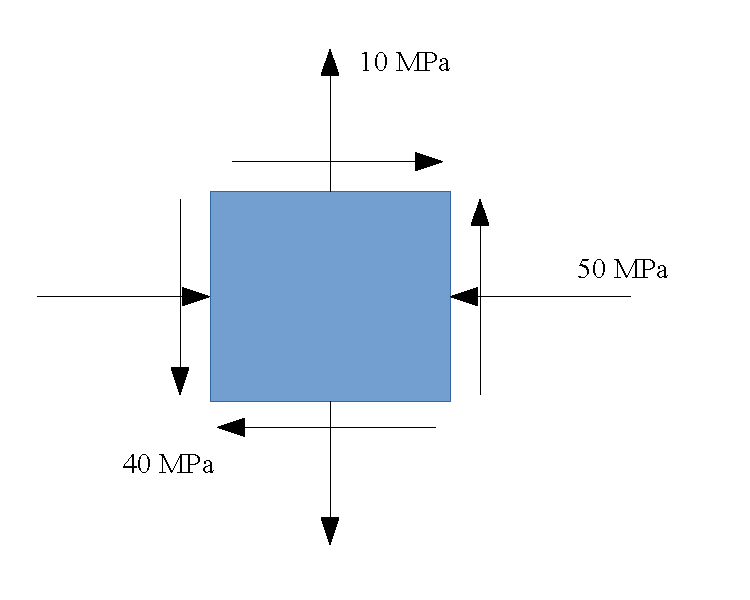
\includegraphics[scale=0.65]{pictures/Static-body-load-analysis/plane-stress-exercise1}
  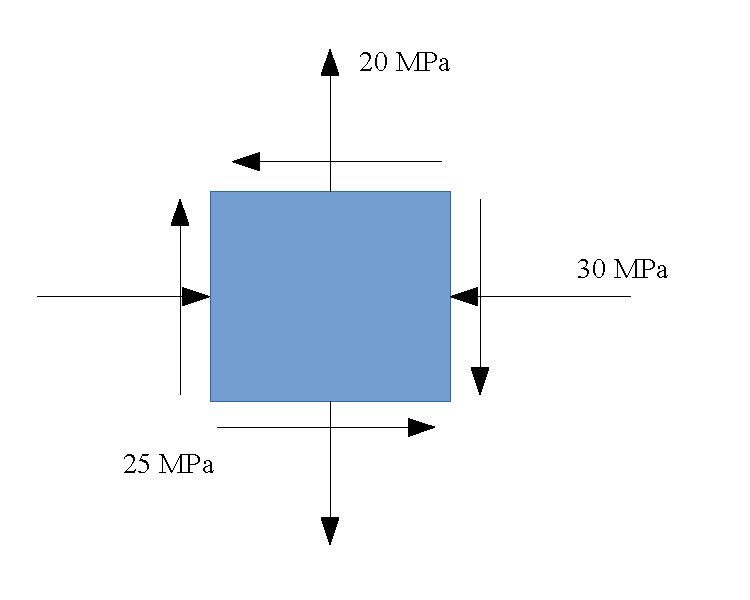
\includegraphics[scale=0.65]{pictures/Static-body-load-analysis/plane-stress-exercise2} \\
  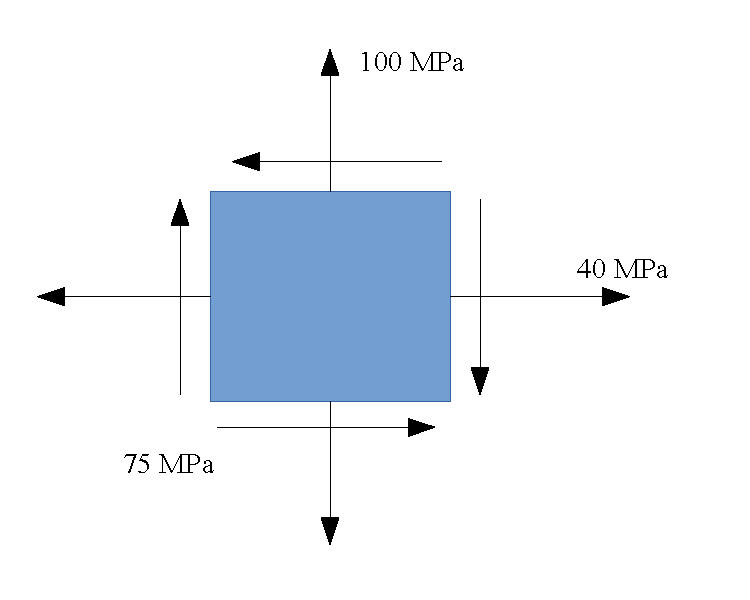
\includegraphics[scale=0.65]{pictures/Static-body-load-analysis/plane-stress-exercise3}

  \item With Mohr's circle, determine the principal stresses, maximum shear stresses, and principal direction for the elements in exercise \ref{exercise: stress transformation}.

  \item A set of strain rosette consisting of strain gages along the $0\degree$, $45\degree$, and 90$\degree$ are attached onto a specimen that undergoes tensile test. The results from the strain gages are $2 \times 10^{-4}$, $1 \times 10^{-4}$, and $ -2 \times 10^{-4}$. Determine the principal strains, the absolute maximum shear strain, and the principal direction.

  \item A $4 \times  4 \times 4$ cm$^3$ cube with $E$ = 200 GPa is put under the
  following state of stress: $\sigma_x$ = 100 MPa, $\sigma_y$ = -50
  MPa, $\sigma_z$ = 80 MPa. After the stresses are applied, the cube's
  volume is increased by 0.05\% compared to its original
  volume. Determine
  \begin{enumerate}
  \item the Poisson's ratio $\nu$ of the cube.
  \item the bulk modulus $K$ of the cube.
  \item the final volume of the cube under a 3D spherical stress of
    -100 MPa. (Remove the original state of stress and apply the
    spherical stress)
  \end{enumerate}

\begin{pycode}
sigma_x = random.randint(-15,15)*10 # -150 - 150 MPa
sigma_y = random.randint(-15,15)*10 # -150 - 150 MPa
tau_xy = random.randint(-15,15)*10 # -150 - 150 MPa
if sigma_x == 0: sigma_x = 80
if sigma_y == 0: sigma_y = -80
if sigma_x == sigma_y: sigma_x = sigma_y + 50
if tau_xy == 0: tau_xy = 60
\end{pycode}

  \item Given a combination of stresses on an element shown in the figure,

        \begin{enumerate}
          \item draw a Mohr's circle representing the complete state of stress of the element, i.e. show prinicpal stresses ($\sigma_{1}, \sigma_{2}$), maximum shear stresses ($\tau_{\max}$), principal direction ($\theta_{p}$), original orientation, and original stresses ($\sigma_{x}, \sigma_{y}, \tau_{xy}$).
          \item draw three-dimensional Mohr's circles showing the three principal stresses and absolute maximum shear stress.
        \end{enumerate}

        \begin{figure}[H]
          \centering
          \begin{tikzpicture}[>=latex]
            \node [draw, minimum height=2cm, minimum width=2cm, fill=LightGrey](element){};
            \begin{pycode}
            if sigma_y > 0:
              print(r'\draw [->, thick] (element.north) --++ (90:1) node[left]{$\sigma_{y}$ = \py{sigma_y} MPa};')
              print(r'\draw [->, thick] (element.south) --++ (-90:1);')
            else:
              print(r'\draw [<-, thick] (element.north) --++ (90:1) node[left]{$\sigma_{y}$ = \py{sigma_y} MPa};')
              print(r'\draw [<-, thick] (element.south) --++ (-90:1);')
            if sigma_x > 0:
              print(r'\draw [->, thick] (element.east) --++ (0:1) node[above right]{$\sigma_{x}$ = \py{sigma_x} MPa};')
              print(r'\draw [->, thick] (element.west) --++ (180:1);')
            else:
              print(r'\draw [<-, thick] (element.east) --++ (0:1) node[above right]{$\sigma_{x}$ = \py{sigma_x} MPa};')
              print(r'\draw [<-, thick] (element.west) --++ (180:1);')
            if tau_xy > 0:
              print(r'\draw [-left to, thick] (element.north west) ++ (45:0.3) --++ (0:1.5) node[above right]{$\tau_{xy}$ = \py{tau_xy} MPa};')
              print(r'\draw [-left to, thick] (element.south east) ++ (-135:0.3) --++ (180:1.5);')
              print(r'\draw [-right to, thick] (element.north west) ++ (-135:0.3) --++ (-90:1.5);')
              print(r'\draw [-right to, thick] (element.south east) ++ (45:0.3) --++ (90:1.5);')
            else:
              print(r'\draw [right to-, thick] (element.north west) ++ (45:0.3) --++ (0:1.5) node[above right]{$\tau_{xy}$ = \py{tau_xy} MPa};')
              print(r'\draw [right to-, thick] (element.south east) ++ (-135:0.3) --++ (180:1.5);')
              print(r'\draw [left to-, thick] (element.north west) ++ (-135:0.3) --++ (-90:1.5);')
              print(r'\draw [left to-, thick] (element.south east) ++ (45:0.3) --++ (90:1.5);')
            \end{pycode}
          \end{tikzpicture}
        \end{figure}

        \begin{pycode}
          t = random.randint(2,7)*1e-3 # in mm
          W = random.randint(5,15)/10
          L = random.randint(2,5)
          poisson = random.randint(20,45)/100
          alpha = random.randint(5,15)*1e-6
          T_0 = random.randint(10,45)*10
          T_1 = random.randint(10,45)*10
          T_1 = T_0 + 120 if T_1 == T_0 else T_1
          F = random.randint(20,40)*10000
          E = random.randint(5,25)*10*1e9 # 50 - 250 GPa
        \end{pycode}
  \item A sheet metal whose Poisson's ratio is \py{poisson}, coefficient of thermal expansion is \py{round(alpha/1e-6)} $\times 10^{-6}$ /$^{\circ}$C, $E$ = \py{round(E/1e9)} GPa, with the thickness of \py{round(t/1e-3)} mm, width \py{W} m and length \py{L} m is being stretched uniformly by a force of \py{F} N along its width. Its initial temperature is \py{T_0}$^{\circ}$C and after the process is finished, the temperature is cooled down to \py{T_1}$^{\circ}$C, determine the percentage volume change of the sheet from the initial, unstressed state.

        \begin{figure}[htbp]
          \centering
          \begin{tikzpicture}[>=latex]
            \node[minimum height=3cm,minimum width=4cm, draw, fill=LightGrey](sheet){};
            \foreach \x in {0,1,...,6} {
              \draw [->, thick] (sheet.south east) ++ (90:0.5*\x) --++ (0:1);
              \draw [->, thick] (sheet.south west) ++ (90:0.5*\x) --++ (180:1);
            }
            \node at (sheet.east) [xshift=1.7cm]{\py{F} N};
            \draw [|<->|] (sheet.north west) ++ (90:0.3) --++ (0:4) node[midway, fill=White]{\py{L} m};
            \draw [|<->|] (sheet.north west) ++ (180:1.5) --++ (-90:3) node[midway, fill=White]{\py{W} m};
          \end{tikzpicture}
        \end{figure}
\end{exercises}
    
%%%%%%%%%%%%%%%%%%%%%%%%%%%%%%%%%%%%%%%%%%%%%%%%%%%%%%%%%%%%%%%%%%%%%%%%%%%%%%%%%%%%%%%%%%%%%%%%%%%%%%%%%%%%%%%%%%%%%%%%%%%%%%%%%%%%%%%%%%%%%%%%%%%%%%%%%%%%%%%%%%%%%%%%%%%%%%

\chapter{Analysis of Members under Combined Loadings}

Many members and structures in actual engineering applications are subjected to multiple simultaneous loadings. In this chapter, we will combine what we have discussed in previous chapters to determine stress distributions and deformations of members under combined loadings.

\section{Thin-Walled Pressure Vessels}

Cylindrical or spherical vessels are commonly used in industry to serve as boilers and tanks. When under pressure, the material of which they are made is subjected to a loading from all directions. Although this is the case, the vessel can be analyzed in a simpler manner provided it has a thin wall, meaning its wall thickness is much smaller than its radius of curvature.

When the vessel wall is thin, the stress distribution throughout its thickness will not vary significantly, and so we will assume that it is uniform or constant. Using this assumption, we will now analyze the state of stress in thin-walled cylindrical and spherical pressure vessels. The pressure in both cases is understood to be the \emph{gauge pressure}—the pressure above the atmospheric pressure.

\subsection{Cylindrical vessels}

\begin{marginfigure}
  \centering
  \begin{tikzpicture}[scale=2, view angle=15, >=latex]
    % Back of sphere
    \draw[left color=brown!50, right color=brown, horizontal] (0,0) --++ (-120:2) arc (-120:-300:1);
    % Front of sphere
    \draw[left color=brown, right color=brown, middle color=brown!50, horizontal] (0,0) --++ (-90:4.5) node(B){} --++ (-120:2) node(A){} --++ (90:4.5);
    \draw[left color=brown!50, right color=brown, horizontal] (A.center) arc (-120:-180:1) --++ (90:4.5) arc (-180:-120:1);
    % arrows
    \foreach \x in {0,1.1,2.2,...,4.4} {
      \draw [horizontal, ->, thick] (A.center) ++ (90:\x) --++ (-30:0.5);
      \draw [horizontal, ->, thick] (B.center) ++ (90:\x) --++ (-30:0.5);
    }
  \end{tikzpicture}
  % 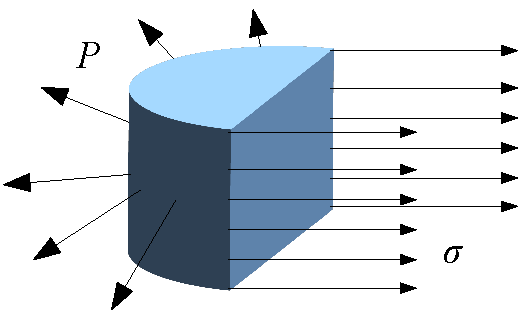
\includegraphics[scale=0.7]{pictures/Combined-loadings/cylindrical-vessel-circ}
  \caption{Force balance between the circumferential stress in vessel's wall and internal pressure.}
  \label{fig: cylindrical vessel circumferential}
\end{marginfigure}

Consider the vessel having a wall thickness $t$ and inner radius $r$. A gauge pressure $p$ is developed within the vessel by a contained gas or fluid, which is assumed to have negligible weight. Due to the uniformity of this loading, the wall is subjected to normal stresses $\sigma_c$ in the circumferential or hoop direction and $\sigma_l$ in the longitudinal or axial direction. Both of these stress components exert tension on the material. To determine the stress components, we will apply the method of sections and the equations of force equilibrium. For the hoop stress, consider the vessel to be sectioned perpendicular to its axis and in half as shown in \cref{fig: cylindrical vessel circumferential}.

\begin{marginfigure}
  \centering
  \begin{tikzpicture}[>=latex]
    \node [draw, cylinder, left color=brown, right color=brown, middle color=brown!50, minimum height=3cm, minimum width=3cm, inner sep=10, rotate=90](cyl){};
    \node at (cyl.east) [anchor=north, fill=brown!50, ellipse, minimum width=3cm, minimum height=0.7cm](top){};
    \draw [->, very thick](top.north) --++ (90:1);
    \draw [->, very thick](top.north east) --++ (90:1);
    \draw [->, very thick](top.east) --++ (90:1);
    \draw [->, very thick](top.south east) --++ (90:1);
    \draw [->, very thick](top.south) --++ (90:1);
    \draw [->, very thick](top.north west) --++ (90:1);
    \draw [->, very thick](top.west) --++ (90:1);
    \draw [->, very thick](top.south west) --++ (90:1);
  \end{tikzpicture}
  % 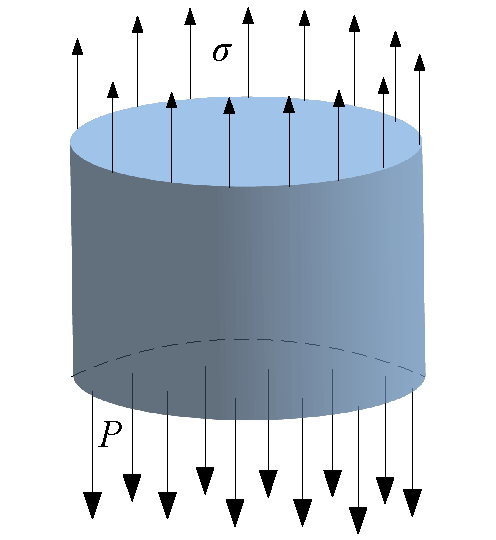
\includegraphics[scale=0.7]{pictures/Combined-loadings/cylindrical-vessel-long}
  \caption{Force balance between longitudinal stress and internal pressure.}
  \label{fig: cylindrical vessel longitudinal}
\end{marginfigure}

Considering only the loading in $x$ direction, the pressure on the wall surface must be balanced by the hoop stress throughout the thickness of both walls. The total force from pressure on the wall surface is the same as the force on the vertical face of the sectioned vessel content. Therefore, we have

\begin{equation}
  \begin{gathered}
    2\sigma _ctdy - p(2r)(dy) = 0 \\ 
    {\sigma _c} = \frac{pr}{t} \\ 
  \end{gathered}
\end{equation}

In order to obtain the longitudinal stress $\sigma_l$, we will consider the left portion the vessel as it is sectioned in the middle of the cylinder.

Consider the force in the $y$ direction, we have

\begin{equation}
  \begin{gathered}
    {\sigma _l}(2\pi rt) - p(\pi {r^2}) = 0 \\ 
    {\sigma _l} = \frac{pr}{2t} \\ 
  \end{gathered}
\end{equation}

It should be noted that the hoop stress is twice as large as the longitudinal stress.

\subsection{Spherical Vessels}

We can analyze a spherical vessel in a similar manner. Consider the vessel that has a wall thickness $t$ and inner radius $r$ and is subjected to an internal gauge pressure of $p$. If the vessel is sectioned in half, the resulting free body diagram illustrated in \cref{fig: spherical vessel} shows that the force resultant from pressure on the wall surface must be balanced by the force resultant from the circumferential or hoop stress. Thus, we have

\begin{marginfigure}
  \centering
  \begin{tikzpicture}[scale=2, view angle=15]
    % Back of sphere
    \draw[fill=brown!50, fill opacity=.75, horizontal] (0,0) circle (1);
    % Front of sphere
    \draw[left color=brown, right color=brown, middle color=brown!50, fill opacity=.75] (0:1) arc (0:-180:1) [horizontal] node[at start](A){} node[near start](B){} node[midway](C){} node[near end](D){} node[at end](E){} arc (-180:0:1) ;
    % Other stuff
    \foreach \n in {1,...,8} {
      \draw [vertical at=45*\n+10,->, very thick] (0:1) --++ (90:0.4);
    }
    \draw [->, very thick] (A.center) --++ (0:0.4);
    \draw [->, very thick] (B.center) --++ (-45:0.4);
    \draw [->, very thick] (C.center) --++ (-90:0.4);
    \draw [->, very thick] (D.center) --++ (-130:0.4);
    \draw [->, very thick] (E.center) --++ (-180:0.4);
  \end{tikzpicture}
  % 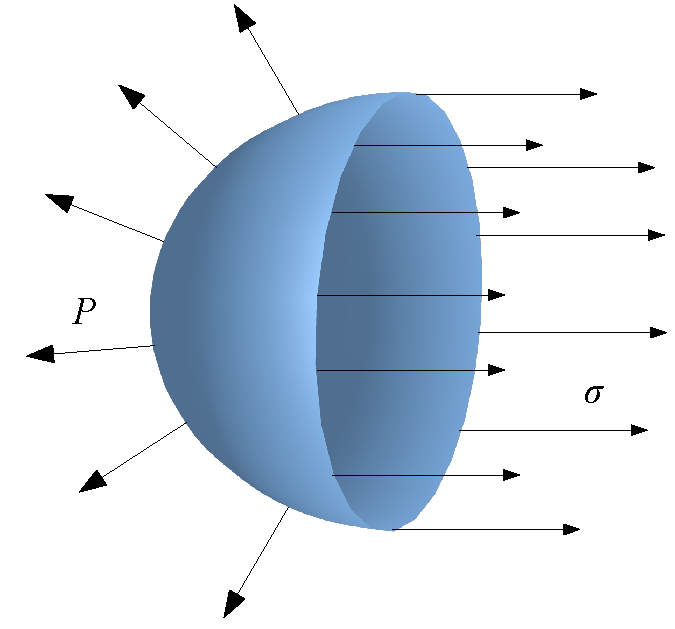
\includegraphics[scale=0.6]{pictures/Combined-loadings/spherical-vessel}
  \caption{Force balance between the circumferential stress in spherical vessel's wall and internal pressure.}
  \label{fig: spherical vessel}
\end{marginfigure}

% \tdplotsetmaincoords{70}{120}
% \tdplotsetrotatedcoords{90}{90}{90}
% \begin{figure}[h]
%   \centering
%   \begin{tikzpicture}[tdplot_main_coords,scale=0.5]
%     \tdplotsetrotatedcoords{90}{90}{90}%
    
%     \draw (0,0,0)--++(0,-2.3,0)node[above left]{$-$};

%     % draw condensore plate
%     \draw[fill=lightgray] (-1.5,0,-1.5)--(-1.5,0,1.5)--(1.5,0,1.5)--(1.5,0,-1.5)--cycle;
%     \draw[fill=lightgray] (1.5,0,-1.5)--(1.5,-0.2,-1.5)--(1.5,-0.2,1.5)--(1.5,0,1.5)--cycle;
%     \draw[fill=lightgray] (1.5,-0.2,1.5)--(-1.5,-0.2,1.5)--(-1.5,0,1.5)--(1.5,0,1.5)--cycle;

%     % draw surface
%     \def\q{-2.3}
%     \def\R{3}
%     \draw (0,-0.5*\q,0) coordinate(R);
%     \tdplotdrawarc[tdplot_rotated_coords,fill=lightgray,fill opacity=0.5,draw=black]{(R)}{\R}{0}{360}{}{}
%     \draw[tdplot_rotated_coords](R)++(-110:\R) node[below left]{$S_1$};
%     \draw[tdplot_rotated_coords](R)++(70:\R) node[above right]{$C$};
%     \tdplotsetrotatedcoords{0}{70}{90}
%     \draw[tdplot_rotated_coords](R)++(90:\R) coordinate (A) circle(0.5pt);
%     \draw[tdplot_rotated_coords,fill opacity=0.5,fill=lightgray!30](A)arc(90:270:\R);
%     \tdplotsetrotatedcoords{90}{90}{90}
%     \tdplotdrawarc[tdplot_rotated_coords,fill=lightgray!10,draw=black]{(R)}{\R}{0}{360}{}{}
%     \begin{scope}

%     % draw condensor plate again, inside (clip outside)
%     \clip[tdplot_rotated_coords] (R)++(0:\R) arc (0:360:\R);
%     \draw[fill=lightgray] (-1.5,0,-1.5)--(-1.5,0,1.5)--(1.5,0,1.5)--(1.5,0,-1.5)--cycle;
%     \draw[fill=lightgray] (1.5,0,-1.5)--(1.5,-0.2,-1.5)--(1.5,-0.2,1.5)--(1.5,0,1.5)--cycle;
%     \draw[fill=lightgray] (1.5,-0.2,1.5)--(-1.5,-0.2,1.5)--(-1.5,0,1.5)--(1.5,0,1.5)--cycle;
%     \end{scope}
%     \draw[tdplot_rotated_coords] (R)++(0:\R) arc (0:360:\R);

%     % draw second condensor plate
%     \draw[fill=lightgray] (-1.5,0-\q,-1.5)--(-1.5,0-\q,1.5)--(1.5,0-\q,1.5)--(1.5,0-\q,-1.5)--cycle;
%     \draw[fill=lightgray] (1.5,0-\q,-1.5)--(1.5,-0.2-\q,-1.5)--(1.5,-0.2-\q,1.5)--(1.5,0-\q,1.5)--cycle;
%     \draw[fill=lightgray] (1.5,-0.2-\q,1.5)--(-1.5,-0.2-\q,1.5)--(-1.5,0-\q,1.5)--(1.5,0-\q,1.5)--cycle;
%     \draw (0,-\q,0)--++(0,2,0)node[above right]{$+$};
%   \end{tikzpicture}
% \end{figure}

\begin{equation}
  \begin{gathered}
    {\sigma }(2\pi rt) - p(\pi {r^2}) = 0 \\ 
    {\sigma } = \frac{{pr}}{{2t}} \\ 
  \end{gathered}
\end{equation}

By comparison, this is the same result obtained for the longitudinal stress in the cylindrical pressure vessel. Furthermore, this stress will be the same regardless of the orientation on the hemispheric free body diagram.

\begin{example}
A thin-walled cylindrical pressure vessel with thickness of 3 mm and diameter of 30 cm is pressurized with natural gas. If the vessel material has the maximum allowable stress of 100 MPa, what is the maximum pressure that the vessel can withstand?
\end{example}
\begin{solution}
The stresses on cylindrical pressure vessels due to internal pressure are always principal stresses. Therefore, we need only compare the maximum allowable stress to the maximum principal stress on the vessel, which is always the hoop/circumferential stress.

\begin{align*}
  {\sigma _c} &= \frac{{Pr}}{t} \\ 
  P &= \frac{{{\sigma _{\max }}t}}{r} \\ 
              &= \frac{100 \times 10^6 \times 3 \times 10^{ - 3}}{30 \times 10^{ - 2}} \\ 
              &= {10^6} \text{ Pa} = 1\text{ MPa} \\ 
\end{align*}

\end{solution}
\section{State of Stress Caused by Combined Loadings}

We have discussed the methods for determining stress distributions in a member subjected to an internal axial force, a shear force, a bending moment, or a torsional moment. In reality, however, the cross section of a member is subjected to several of these types of loadings simultaneously, and as a result, the method of superposition, if it applies, can be used to determine the resultant stress distributions caused by the loads. It must be noted that the principle only applies when there is a \emph{linear relationship} between the \emph{stress} and the \emph{loads} and when the member does not undergo significant deformation due to the loads.

Problems with multiaxial stress usually involves
\begin{enumerate}
\item a critical member with multiple loadings, each of which leads to a resultant stress. \emph{or}
\item a member with a single load, but due to the geometry of the member, the load causes multiple types of loading \emph{or}
\item a combination of the previous two.
\end{enumerate}

Analysis of these problems involves first identify the critical point on the member. Keep in mind that we use the word `point' loosely here. The actual critical `point' can in reality be more than one point, or may contain an entire surface or the volume of the component.

\begin{example} A helicopter rotor shaft design

  We want to determine the proper diameter of a rotor shaft for a 4-ton helicopter. The shaft is connected to the engine that provides the maximum torque of 8000 N-m. The shaft is made of AISI1023 steel with $\sigma_{allow}$ = 400 MPa.

  \begin{figure}[H]
    \centering
    \begin{tikzpicture}[>=latex]
      \node [draw, cylinder, fill=Gray!80, minimum height=1cm, minimum width=0.5cm, shape border rotate=90, inner sep=1pt] (shaft){};
      \node at (shaft.north) [anchor=east, yshift=-0.5mm, draw, fill=LightGray, ellipse, minimum height=0.4cm, minimum width=5cm](left){};
      \node at (shaft.north) [anchor=west, yshift=-0.5mm, draw, fill=LightGray, ellipse, minimum height=0.4cm, minimum width=5cm](right){};
      \draw [->>, ultra thick] (shaft.south) --++ (-90:1) node[right]{$T = 8000$ N-m};
      \draw [->, ultra thick] (shaft.south) --++ (-90:2) node[right]{$W = 4$ ton};
    \end{tikzpicture}
  \end{figure}

\end{example}
\begin{solution}
  First of all, we must determine the location of a critical point. The applied load on the shaft are the torque from the engine and the weight of the helicopter. The axial load of the weight does not give any maximum stress location, while the torsion from the engine means that the outer surface is carrying the highest shear stress. Combining the two, the outer surface of the shaft is the critical `surface.' We can the substitute the loads to determine the stress.

  \begin{align*}
    \sigma &= \frac{F}{A} = \frac{4(1000 \text{ kg/ton})(10 \text{ N/kg})}{\pi r^2} \\
           &= \frac{12732}{r^2} \\
    \tau &= \frac{Tr}{J} = \frac{8000(r)}{\pi r^4/2} \\
           &= \frac{5093}{r^3}
  \end{align*}

  So the state of stress at the critical surface is a combination of normal stress and shear stress. Since the given material is limited by its normal stress, we need to determine the maximum principal stress.

  \begin{align*}
    \sigma_1 = \sigma_{allow} = 400 \times 10^6 &= \frac{12732}{2r^2} + \sqrt{ \left( \frac{12732}{2r^2} \right)^2 + \left( \frac{5093}{r^3} \right)^2 }
  \end{align*}

  This equation can be solved numerically to obtain $r = 2.38$ cm.
\end{solution}
 
\section*{Summary}

In this chapter, the concept in Chapter 6 is utilized. In the first part, one of the simplest and most used applications of multiaxial stress analysis is introduced: pressure vessels. We analyzed the principal stresses and maximum shear stresses depending on the internal pressure and vessel dimensions. In the second part, we open up to all types of possible problems which lead to multiaxial stress state: combined loadings. The key is to determine the types of loads on the cross section--whether forces or moments, determine the resulting stresses, and use the multiaxial stress analysis to determine the principal stresses and maximum shear stress.

\section*{Exercise}

\begin{exercises}

  \item \label{exercise: cantilever beam} A cantilever beam of rectangular cross section is subjected to a concentrated load $P$ = 75000 N acting at the free end. The beam has width $b$ = 10 cm and height $h$ = 25 cm. Point A is located at distance $c$ = 60 cm from the free end and distance $d$ = 8 cm from the bottom of the beam. Calculate the principal stresses 1 and 2 and the maximum shear stress max at point A.
  \begin{figure}[h]
    \centering
    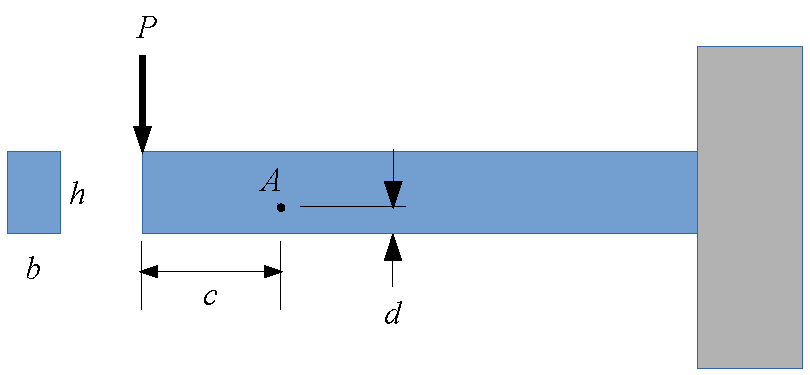
\includegraphics[scale=0.7]{pictures/Static-body-load-analysis/multiaxial-cantilever-beam-exercise}
    \caption{Exercise \ref{exercise: cantilever beam}}
  \end{figure}
  
  \item \label{exercise: generator shaft}A generator shaft of hollow circular cross section is subjected to a torque T = 25 kN-m. The outer and inner diameters of the shaft are 200 mm and 160 mm, respectively. What is the maximum permissible compressive load $P$ that can be applied to the shaft if the allowable in-plane shear stress is allow = 45 MPa?
  
  \begin{figure}[h]
    \centering
    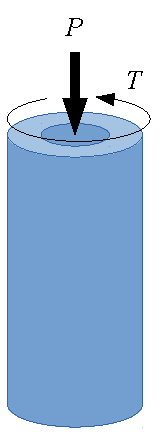
\includegraphics[width=0.3\textwidth]{pictures/Static-body-load-analysis/multiaxial-generator-shaft-exercise}
    \caption{Exercise \ref{exercise: generator shaft}}
  \end{figure}
  
  \item A machine shaft of solid circular cross section is being designed for a tensile load $P$ = 80 kN and a torque $T$ = 1.1 kN-m. The allowable stresses are 60 MPa in tension and 30 MPa in shear. What is the required diameter of the shaft?

  \item A segment of a cylindrical pressure vessel is subjected to a torque T and bending moment M as shown. The outer radius is 12 in and the wall thickness is 1 in. The loads are as follows: T = 8x105 lb-in, M = 106 lb-in, and the internal pressure p = 900 psi. Determine the maximum tensile stress, maximum compressive stress, and maximum shear stress in the wall of the cylinder.

  \item A thin-walled cylindrical pressure vessel of 10 cm radius and 0.25 cm thickness is working with the inside pressure $p$. The vessel is also loaded by an axial force of $F$. The vessel is made of steel, which has yield stress
  \begin{enumerate}
  \item If F = 40 kN, what is the pressure p so that the vessel is beginning to yield under the maximum distortional energy criterion?
  \item If p = 2 MPa, what is the axial load F so that the vessel is beginning to yield under the maximum normal stress criterion?
  \end{enumerate}

  \item You made a bet with your friend that you can apply a large enough bending moment to break an unopened coke can. The can is assumed to be a cylindrical thin-walled vessel whose radius $r$ is 2.5 cm and wall thickness $t$ is 0.3 mm. The internal gage pressure of the can is 100 kPa. The can is made of aluminum whose $\sigma_{allow}$ = 100 MPa. Determine how much bending moment you must apply in order to win this bet.
  
  Note: the moment of inertia of a cylindrical thin-walled vessel is $I = 3 \pi r^3 t$.

  \item You are chewing a bubblegum that has a volume of 2 cm$^3$ and blowing a bubble. Assume that the bubble forms a thin-walled sphere with a constant internal pressure of 3 kPa, regardless of the size of the bubble. What is the maximum radius, $r$, of the bubble that you can blow given that the maximum allowable normal stress of the gum is 50 kPa?
    
    Note: You may assume that the volume of gum used to blow a spherical bubble of radius $r$ and thickness $t$ is $4\pi r^2 t$ and that the volume of the gum always remains 2 cm$^3$.

  \item A 500-N highway sign is attached to the end of an L-shaped, massless pole. The AISI-1023 steel pole (a ducile material with $E$ = 200 GPa and $S_y$ = 360 MPa) is a constant cross-sectioned tube whose outer radius of the pole $r_o$ is 10 cm. Determine

  \begin{enumerate}
  \item the critical point of the pole. (Hint: be specific. Don't just say `the end of the pole.' Point to the exact location of the critical point.) Explain your reasoning.
  \item maximum possible inner diameter $r_i$.
  \end{enumerate}
  
\item An L-shaped bar is fixed on one end at the wall. The bar has a constant circular cross section with the radius of 1 cm. The bar is made of a \emph{ductile} steel whose Young's modulus $E$ = 210 GPa, yield strength $S_{yield}$ = 300 MPa, and ultimate tensile strength $S_{ut}$ = 450 MPa.

  \begin{center}
    \begin{tikzpicture}[>=latex]
      \node [trapezium, trapezium left angle=115, trapezium right angle=65, pattern=north west lines, minimum height=1cm, rotate=90]{};
      \draw [thin, Black, double=LightGrey, double distance=12pt, rounded corners=5mm, line cap=round] (0,0) node(A){} --++ (-25:6) node(B){} --++ (-155:4) node(C){};
      \draw [->, thick] (B.center) ++ (0:2) node(D){} --++ (-25:1) node[right]{$y$};
      \draw [->, thick] (D.center) --++ (90:1) node[above]{$z$};
      \draw [->, thick] (D.center) --++ (-155:1) node[below left]{$x$};
      \draw [<->] (A.center) ++ (25:0.7) --++ (-25:6) node[midway, fill=white, rotate=-25]{80 cm};
      \draw [<->] (C.center) ++ (-25:0.7) --++ (25:4) node[midway, fill=white, rotate=25]{50 cm};
      \node at (C.center) [draw, very thin, fill=LightGrey!50, circle, minimum height=12pt](E){};
      \draw [<-, very thick] (E.north) --++ (90:1) node[above]{$P$};
    \end{tikzpicture}
  \end{center}

  \begin{enumerate}
  \item (5 points) Determine the location of a critical point. (Be specific.)
  \item (5 points) Draw a Mohr's circle representing the state of stress (principal and maximum shear stresses) at the critical point.
  \item (5 points) Determine the maximum static (constant) load $P$ that can be exerted on the bar.
  \item (5 points) Determine the maximum repeated and fully reversed load that varies back and forth between $-P$ and $P$ that can be exerted on the bar.
  \end{enumerate}

\begin{pycode}
sigma_allow = random.randint(3,15)*10*1e6 # 30 - 150 MPa
tau_allow = random.randint(2,10)*10*1e6 # 20 - 100 MPa
r = random.randint(15,25)/10*1e-2 # 1.5 - 2.5 cm
t = random.randint(3,10)/10*1e-3 # 0.3 - 1 mm
h = random.randint(4,7)*1e-2 # 4 - 7 cm
p0 = round(random.randint(1,5)*1e3) # 1 - 5 kPa
\end{pycode}

  \item You want to play a prank on your friend by shaking a can of coke and let him open it so that the can would spray all over him. You want to make sure, however, that the can would not explode before said prank is complete. The can is made of aluminum whose allowable normal stress is $\sigma_{\text{allow}}$ = \py{round(sigma_allow/1e6)} MPa and allowable shear stress is $\tau_{\text{allow}}$ = \py{round(tau_allow/1e6)} MPa. The can dimensions are $r$ = \py{round(r/1e-2,1)} cm, $h$ = \py{round(h/1e-2)} cm, and wall thickness $t$ = \py{round(t/1e-3,1)} mm. Each time you shake, the pressure build up following a function:

        \begin{align*}
          p = (\py{p0})1.2^{n}
        \end{align*}
        where $p$ is the pressure in Pa and $n$ is the number of times you shake the soda can. Determine how many times you can shake the can without ruining your own prank.

\begin{pycode}
F = random.randint(10,30)*100 # 1000 - 3000
L1 = random.randint(15,30)/10 # 1.5 - 3 m
x = L1 - random.randint(5,10)/10 # 0.5 - 1 m
frac = x/L1
d = round(random.randint(2,4)/5*L1,3)
frac_d = d/L1
L2 = random.randint(5,10)/10 # 0.5 - 1 m
b = random.randint(3,8)*1e-2 # 3 - 8 cm
h = random.randint(2,7)*1e-2 # 2 - 7 cm
frac_bh = b/h
\end{pycode}

  \item A structure shown in the figure below is loaded with a downward force. Determine the state of stress of point C by drawing a Mohr's circle.

        \begin{figure}[htbp]
          \centering
          \begin{tikzpicture}[>=latex]
            \node[minimum height=1cm, minimum width=5mm, pattern=north west lines](wall){};
            \draw (wall.north east) -- (wall.south east);
            \node at (wall.east) [anchor=south, rotate=-90, draw, regular polygon, regular polygon sides=3,minimum height=5mm, inner sep=0](support){};
            \draw [Black, line cap=rect, double=LightSkyBlue, double distance=10pt] (support.north) --++ (0:4) node(elbow){} --++ (30:2) node [draw, circle, inner sep=0, minimum height=2mm, yshift=-2mm, xshift=2.5mm](rsupport){};
            \node at (support.north) [draw,circle, inner sep=0, minimum height=1mm]{};
            \node at (rsupport.south east) [anchor=north, pattern=north east lines, minimum height=5mm, minimum width=1cm, rotate=30](rwall){};
            \draw (rwall.north east) -- (rwall.north west);
            \begin{pycode}
            print(r'\draw [<-, ultra thick] (support.north) ++ (0:'+str(frac*4)+r') ++ (90:0.2) --++ (90:1) node[above]{\py{F} N};')
            print(r'\draw [|<->|] (support.north) ++ (90:0.5) --++ (0:'+str(frac*4)+r') node[midway, fill=White]{\py{round(x,1)} m};')
            print(r'\node at (support.north) [draw, fill=Black, circle, inner sep=0, minimum height=1mm,yshift=-2mm,xshift='+str(4*frac_d)+r'cm](C){};')
            print(r'\draw [|<->|] (support.north) ++ (-90:0.5) --++ (0:'+str(frac_d*4)+r') node[midway, fill=White]{'+str(d)+r' m};')
            \end{pycode}

            %%% sectional arrow %%%%
            \draw [<->] (support.north) ++ (0:3.8) ++ (-90:0.5) ++ (180:0.3) node[left]{A} --++ (0:0.3) --++ (90:1) --++ (180:0.3) node[left]{A};

            %%%%% sectional view %%%%%
            \begin{pycode}
              print(r'\node at (wall.west) [draw, xshift=-2cm, minimum height='+str(1.5/frac_bh)+r'cm, minimum width=1.5cm, fill=LightSkyBlue](section){};')
              print(r'\draw [|<->|] (section.south west) ++ (180:0.3) --++ (90:'+str(1.5/frac_bh)+r') node[midway, left, fill=White]{'+str(round(h/1e-2))+r' cm};')
            \end{pycode}
            \draw [|<->|] (section.south west) ++ (-90:0.3) --++ (0:1.5) node[midway, fill=White]{\py{round(b/1e-2)} cm};
            \node at (section.south) [below,yshift=-5mm] {section A-A};
            \node at (C.center) [above right]{C};
            \draw [|<->|] (support.north) ++ (-90:1) --++ (0:4) node[midway, fill=White]{\py{L1} m};
            \draw [dashed] (elbow.center) ++ (-90:5pt) --++ (0:2) node[midway,above]{30$^{\circ}$};
            \draw [|<->|] (elbow.center) ++ (100:15pt) --++ (30:2) node[midway, fill=White, rotate=30]{\py{L2} m};
          \end{tikzpicture}
        \end{figure}

\end{exercises}

%%%%%%%%%%%%%%%%%%%%%%%%%%%%%%%%%%%%%%%%%%%%%%%%%%%%%%%%%%%%%%%%%%%%%%%%%%%%%%%%%%%%%%%%%%%%%%%%%%%%%%%%%%%%%%%%%%%%%%%%%%%%%%%%%%%%%%%%%%%%%%%%%%%%%%%%%%%%%%%%%%%%%%%%%%%%%%%%%%%%%%%%%%%%%%%%%%%%%%%%%%%%%%%%%%%%%%%%%%%%%%%%%%%%%%%

\chapter{Energy Method}

In this chapter, a different approach of solving deflection and deformation problems using energy methods. In kinetics and kinematics problems, problems can be solved using either the equations of motions to relate loads to acceleration, velocity, and displacements or the energy approach relating potential and kinetic energy to determine the answers. The alternated energy approach can also be applied to problems of mechanics of materials where there are little to no macroscale displacement of the body.

To understand the application of energy method to solving mechanics of materials problems, we will discuss external work and corresponding strain energy in solid members, which are related by the principle of conservation of energy. Using this, deflection resulted from impact loadings can be determined. Afterwards, we will develop the method of virtual work and Castigliano's theorem, which can be used to determine the displacement and slope on structural members and mechanical components.

\section{** Mechanical Work **}

We can determine deflections of any point on a truss, beam, or shaft using the energy methods. To derive that relationship, we must first understand the process of how energy is stored in a deformable body and its relation to external work caused by exerted loads. We will formulate the equation which will be used as a basis for work and strain energy throughout this chapter.

\paragraph{Work of a force.}

If you recall from physics, a force $F$ does work only if it undergoes displacement $dx$ in the same direction as itself. If we translate that into an equation, we will have that the work $U$ done by the force $F$ over a displacement $x$ is

\begin{figure}[h]
  \centering
  \begin{tikzpicture}
    \node [draw, rectangle, left color=SkyBlue, right color=SkyBlue, middle color=SkyBlue!50, minimum height=3cm, minimum width=5mm](bar){};
    \node at (bar.north) [anchor=south, pattern=north east lines, minimum height=5mm, minimum width=2cm](ceilleft){};
    \draw (ceilleft.south west) -- (ceilleft.south east);
    \node at (bar.north) [anchor=north, dashed, draw, rectangle, minimum height=3.5cm, minimum width=5mm](ebar){};
    \draw [->, thick](ebar.south) --++ (-90:1) node[left]{$P$};
    \draw [|->|] (bar.south east) ++ (0:0.3) --++ (-90:0.5) node[midway, right]{$\delta$};
    \node at (bar.north) [anchor=north, xshift=4cm, draw, rectangle, left color=SkyBlue, right color=SkyBlue, middle color=SkyBlue!50, minimum height=3.5cm, minimum width=5mm](rbar){};
    \node at (rbar.north) [anchor=south, pattern=north east lines, minimum height=5mm, minimum width=2cm](ceilright){};
    \draw (ceilright.south west) -- (ceilright.south east);
    \node at (rbar.north) [anchor=north, dashed, draw, rectangle, minimum height=3.8cm, minimum width=5mm](erbar){};
    \draw [|->|] (rbar.south east) ++ (0:0.3) ++ (90:0.5) --++ (-90:0.5) node[midway, right]{$\delta$};
    \draw [|->|] (rbar.south east) ++ (0:0.3) --++ (-90:0.3) node[midway, right]{$\delta'$};
    \draw [->, thick](rbar.south) --++ (-90:1) node[right]{$P$};
    \draw [->, thick](erbar.south) ++ (180:0.2) --++ (-90:0.5) node[left]{$P'$};
  \end{tikzpicture}
\end{figure}


\begin{equation} \label{eqn: force-work equation}
  U = \int_0^x F dx
\end{equation}

Now, consider the application of the equation in reality. Let us calculate the work done by an axial force applied to the end of a bar. The magnitude of the force is slowly increased from zero to $P$ where the elongation of the bar is $\delta$. If the material behaves in a linear elastic manner, the force is directly proportional to the elongation, i.e. $F = (P/\delta)x$. Substitute this equation into \cref{eqn: force-work equation}, we have

\begin{equation}
  U = \frac{1}{2} P \delta
\end{equation}

\begin{marginfigure}
  \centering
  \begin{tikzpicture}
    \draw [->] (0,0) --++ (0:4) node[right]{$x$};
    \draw [->] (0,0) --++ (90:5) node[above]{$F$};
    \draw [fill=LightBlue!40] (0,0) --++ (50:3) node(A){} --++ (-90:3*sin(50) node(B){} node[below]{$\delta$} node[below, xshift=1.3cm]{$\delta'$} -- cycle;
    \draw [fill=LightGrey!80] (A.center) --++ (50:2) node(C){} --++ (-90:2*sin(50) node(D){};
    \draw [fill=SkyBlue] (B.center) rectangle (D.center);
    \draw [dashed] (A.center) --++ (180:3*cos(50) node[left]{$P$};
    \draw [dashed] (C.center) --++ (180:5*cos(50) node[left]{$P'$};
  \end{tikzpicture}
  \caption{Force-deformation diagram for a linearly elastic bar.}
  \label{fig:force-deformation diagram}
\end{marginfigure}

As the force is applied to the bar, its magnitude builds from 0 to $P$, and the work done by that force is equal to the average force magnitude $P/2$ multiplied by the total displacement $\delta$. This can be represented graphically as the light-blue shaded area of the triangle in \cref{fig:force-deformation diagram}.

Now, if there is an additional force $P'$ applied at the end of the bar and further displaced it by $\delta'$, the work done by $P'$ is equal to the shaded triangular area, by the work done by $P$ under goes this further displacement is

\begin{equation}
  U' = P \delta'
\end{equation}

In this case, the work is represented by the dark-blue shaded rectangular area. Since $P$ does not change its magnitude, as the bar's displacement $\delta'$ is only caused by $P'$, the work done by $P$ is simply the force times the displacement $\delta'$.

\paragraph{Work of a Moment.}

Similar to work done by a force, a moment $M$ does work when it causes angular deformation $\theta$ along the same direction. This can be expressed as

\begin{figure}[h]
  \centering
  \begin{tikzpicture}
    \draw [line width=40pt, LightBlue] (0,0) node(A){} arc (110:70:10) node(B){};
    \draw [thick, ->] (A) ++ (135:1) arc (135:270:1) node[midway, fill=white]{$M$};
    \draw [thick, ->] (B) ++ (45:1) arc (45:-90:1) node[midway, fill=white]{$M$};
    \draw [dashed] (A.center) --++ (20:5);
    \draw [dashed] (B.center) --++ (160:3.6) node(C){};
    \draw [->] (C.center) ++ (20:1) arc (20:-20:1) node[midway, right]{$\theta$};
  \end{tikzpicture}
\end{figure}

  \begin{equation}
  U = \int_0^\theta M d\theta
\end{equation}

If the moment is applied to a body having linearly elastic material so that its magnitude slowly increase from zero at $M = 0$ to $M$ at $theta$, then the work done by the moment is

\begin{equation}
  U = \frac{1}{2} M \theta
\end{equation}

However, if the moment is already applied to the body and other loads further rotate the body by $\theta'$, the the additional work done by the moment is

\begin{equation}
  U' = M \theta'
\end{equation}

\section{Strain Energy}

When a material undergoes deformation, given that there is no energy loss to heat, the external work applied is converted and stored in the body as \emph{strain energy}. This energy can be caused by either normal or shear stress.

\subparagraph{Normal Stress.}

If a cube element is subjected to the normal stress $\sigma_x$, then the force created on the element's corresponding faces is $dF_x = \sigma_x dA = \sigma_x dx dy$. If this force is applied slowly, similar to the force $P$ discussed previously, and the element undergoes an elongation $d\delta_x = \varepsilon dx$. The work done by this force is $dU = \frac{1}{2}dF_xd\delta_x = \frac{1}{2} \sigma_xdxdy\varepsilon_xdx$. Since the volume of this cube element is $dV = dxdydz$, we have that 

\begin{equation}
  dU = \frac{1}{2}\sigma_x \varepsilon_x dV
\end{equation}

Note that the strain energy $dU$ is always positive because the directions of force and deformation are always the same. In general, if the element is under a uniaxial normal stress $\sigma$, the corresponding strain energy is

\begin{equation}
  U = \int_V \frac{\sigma \varepsilon}{2} dV
\end{equation}

Also, if the material is linearly elastic, we can apply Hooke's law and express the strain energy as

\begin{equation}
  U = \int_V \frac{\sigma^2}{2E} dV
\end{equation}

\paragraph{Shear Stress.}

A similar strain energy expression can be derived for any material subjected to shear stress as well. Consider the same cube element now under the shear stress on the top face of the element, and is deformed by $\gamma dz$ relative to the bottom face. The resulting shear force is $dF = \tau (dx dy)$. All vertical faces simply rotate, hence the shear force does no work. The strain energy, equal to the work done by the shear force, is

\begin{align}
  dU &= \frac{1}{2} \left[ \tau (dx dy) \right] \gamma dz \nonumber \\
     &= \frac{1}{2} \tau \gamma dV \nonumber \\
  U &= \int_V \frac{1}{2} \tau \gamma dV
\end{align}

Again, shear strain energy is always positive since $\tau$ and $\gamma$ will always be in the same direction. If the material is linearly elastic, then we can apply Hooke's law and write

\begin{equation}
  U = \int_V \frac{\tau^2}{2G} dV
\end{equation}

\paragraph{Multiaxial Stress.}

Expressions for normal and shear strain energy can be expanded to determine the strain energy in a body when it is subjected to multidirectional stresses simultaneously. In fact, since energy is a scalar quantity, the total strain energy can simply be added, giving

\begin{equation}
  U = \int_V \left[ \frac{1}{2}\sigma_x \varepsilon_x + \frac{1}{2}\sigma_y \varepsilon_y + \frac{1}{2}\sigma_z \varepsilon_z + \frac{1}{2}\tau_{xy} \gamma_{xy} + \frac{1}{2}\tau_{xz} \gamma_{xz} + \frac{1}{2}\tau_{yz} \gamma_{yz}\right] dV
\end{equation}

The strains can be substituted with the stresses and their corresponding material properties from Hooke's law, in which we have

\begin{equation}
  U = \int_V \left[ \frac{1}{2E} \left( \sigma_x^2 + \sigma_y^2 + \sigma_z^2 \right) - \frac{\nu}{E} \left( \sigma_x \sigma_y + \sigma_y \sigma_z + \sigma_x \sigma_z \right) + \frac{1}{2G} \left( \tau_{xy}^2 + \tau_{xz}^2 + \tau_{yz}^2 \right) \right] dV
\end{equation}

If the problem has been reduced to the three principal stresses $\sigma_1, \sigma_2, \sigma_3$, the expression is simply

\begin{equation}
  U = \int_V \left[ \frac{1}{2E} \left( \sigma_1^2 + \sigma_2^2 + \sigma_3^2 \right) - \frac{\nu}{E} \left( \sigma_1 \sigma_2 + \sigma_2 \sigma_3 + \sigma_1 \sigma_3 \right) \right] dV
\end{equation}

This equation was used as a basis to derive the maximum distortion energy theory.

\section{Strain Energy for Different Types of Loading}

With the equations developed for normal, shear, and multiaxial strain energy, we can now formulate strain energy stored in members under axial, bending, torsion, and transverse shear loadings.

\paragraph{Axial Load.}

Consider a bar with internal force $F$ and a cross sectional area $A$. At the point of interest, the normal stress is $\sigma = F / A$. Thus, for the strain energy stored in the section, we have

\begin{equation*}
  U = \int_V \frac{\sigma_x^2}{2E} dV = \int_V \frac{F^2}{2EA^2}dV
\end{equation*}

If we choose a thin element with length $dx$ so that $dV = A dx$, then the general equation for the strain energy in an axially loaded bar is

\begin{equation}
  U = \int_0^L \frac{F^2}{2AE} dx
\end{equation}

For a prismatic bar with constant cross-sectional area $A$, length $L$, and axial load $F$, we have

\begin{equation}
  U = \frac{F^2L}{2AE}
\end{equation}

\paragraph{Bending Moment.}

Strain energy equation for bending moment can be developed using the equation for axially loaded members because a bending moment also cause normal stress in the member. For a beam with internal moment $M$ at the location with distance $y$ away from the neutral axis, the normal stress is $\sigma = My/I$. If the volume of the element is $dV = dA dx$, where $dA$ is the small element on the cross section and $dx$ is its length, the strain energy of the beam is

\begin{equation*}
  U = \int_V \frac{\sigma^2}{2E} dV = \int_V \frac{1}{2E} \left( \frac{My}{I} \right)^2 dA dx
\end{equation*}

or

\begin{equation*}
  U = \int_0^L \frac{M^2}{2EI^2} \left( \int_A y^2 dA \right) dx
\end{equation*}

The second integral simply evaluates the moment of inertia of the cross section $I$, so the final expression is

\begin{equation}
  U = \int_0^L \frac{M^2dx}{2EI}
\end{equation}

To determine the strain energy in a beam, it is necessary to express the bending moment along the beam length $x$ and integrate over the entire length.

\paragraph{Transverse Shear.}

The strain energy from shear stress in a beam can be determined using the equation of shear strain energy derived earlier. In this case, we will consider a constant cross-sectioned beam with an axis of symmetry about the $y$ axis. If the internal shear at the cross section is $V$, the shear stress acting on the cross section is $\tau = VQ/Ib$. Sunbstitute into the shear strain energy equation, we have

\begin{align*}
  U &= \int_V \frac{\tau^2}{2G} dV = \int_V \frac{1}{2G} \left( \frac{VQ}{Ib} \right)^2 dA dx \\
  U &= \int_0^L \frac{V^2}{2GI^2} \left( \int_A \frac{Q^2}{b^2} dA \right) dx
\end{align*}

The second integral can be simplified if we define the form factor for transverse shear as

\begin{equation}
  f_s = \frac{A}{I^2} \int_A \frac{Q^2}{b^2} dA
\end{equation}

Substituting the form factor into the equation, we have

\begin{equation}
  U = \int_0^L \frac{f_s V^2 dx}{2GA}
\end{equation}

\paragraph{Torsional Moment.}

Again, since torsion causes shear stress in members, the shear strain energy equation will be applicable. Consider a shaft on which a torque $T$ is applied. The shear stress on the shaft is $T = T \rho / J$. The strain energy stored in the shaft is

\begin{align*}
  U &= \int_V \frac{\tau^2}{2G} dV = \int_V \frac{1}{2G} \left( \frac{T \rho}{J} \right)^2 dA dx \\
    &= \int_0^L \frac{T^2}{2GJ^2} \left( \int_A \rho^2 dA \right) dx
\end{align*}

The area integral represents the polar moment of inertial $J$ for the shaft, and so the equation is simplified to

\begin{equation}
  U = \int_0^L \frac{T^2}{2GJ} dx
\end{equation}

\section{** Principle of Virtual Work **}

Energy methods applied in mechanics rely on conservation of energy. In other words, it is implicitly assumed that work done by external load $W$ is converted and stored purely as strain energy $U$, and that there is no loss to heat, chemical reactions, etc. This is simply expressed as

\begin{equation}
  W = U
\end{equation}

The principal of virtual work is based also on the conservation of energy. It has serveral applications in mechanics, although in this book we will focus on its application to determine displacement and slope on a deformable body.

Let us consider the body to be some random shape subjected to actual loads $P_1, P_2,$ and $P_3$. It is assumed that these loads does not cause any movement of the supports. We want to determine the displacement $\delta$ of point $A$ on the body. As there is no force ating at $A$, $\delta$ is not counted as an \emph{external} work. Thus, we must apply fictitious or \emph{virtual} force $P'$ at point $A$ such that it is pointing in the same direction as $\delta$. We will also assume that the load is applied before any actual loads and that its magnitude is 1.

This external virtual load will create an internal virtual load, similar to the way an external load causes an internal load, which can be determined by the equations of equilibrium. This will cause point $A$ to displace by some virtual amount. Once the actual loads $P_1, P_2,$ and $P_3$ are applied, point $A$ will move by the real amount $\delta$, and the element to be displaced by $dL$. As a result, the external virtual force $P'$ and internal virtual load $u$ are also displaced by $\delta$ and $dL$, respectively. These loads will do external virtual work $1 \cdot \delta$ on the body and internal virtual work $u \cdot dL$ on the element. Considering the conservation of \emph{virtual} energy, the external virtual work and intrenal vertial work must be equal. Therefore, the corresponding virtual work equation is

\begin{equation}
  1 \cdot \delta = \Sigma u \cdot dL
\end{equation}

By choosing the magnitude of external virtual load = 1, the solution for displacement is simply the right side of the equation.

Similarly, we can prove the virtual work and virtual moment relationship to find the slope of point $A$. The corresponding equation is

\begin{equation}
  1 \cdot \theta = \Sigma u_\theta dL
\end{equation}

\paragraph{Internal Virtual Work.}

If we assume that the material behavior is linearly elastic and assume the virtual loads are applied first before any actual loads just like in previous cases, we can write equations for internal virtual work done by virtual force $f$, shear force $v$, bending moment $m$, and torque $t$ on the displacements cause by actual axial load $F$, shear force $V$, bending moment $M$, and torque $T$ as follows.

\begin{table}[h]
  \centering
  \caption{Internal virtual work under various types of deformation.}
  \begin{tabular}{l c c}
    \toprule
    Deformation type & Strain Energy & Internal virtual work \\
    \midrule
    Axial load $F$ & $\displaystyle \int_0^L \frac{F^2}{2EA} dx$ & $\displaystyle \int_0^L \frac{fF}{EA} dx $ \\[2em]
    Shear $V$ & $\displaystyle \int_0^L \frac{f_s V^2}{2GA} dx$ & $\displaystyle \int_0^L \frac{f_s vV}{GA} dx$ \\[2em]
    Bending moment $M$ & $\displaystyle \int_0^L \frac{M^2}{2EI} dx$ & $\displaystyle \int_0^L \frac{mM}{EI} dx$ \\[2em]
    Torque $T$ & $\displaystyle \int_0^L \frac{T^2}{2GJ} dx$ & $\displaystyle \int_0^L \frac{tT}{GJ} dx$ \\
    \bottomrule
  \end{tabular}
\end{table}

Note that the internal virtual work is \emph{not} multiplied by one half because the virtual load is already assumed fully applied to the member before any actual deformation takes place, resulting in a full quantity of load multiplied by the displacement.

Finally, we can write an expression for a member undergoing multiple types of deformation simultaneously as

\begin{equation}
  1 \cdot \delta = \int_0^L \frac{fF}{EA} dx + \int_0^L \frac{f_s vV}{GA} dx + \int_0^L \frac{mM}{EI} dx + \int_0^L \frac{tT}{GJ} dx
\end{equation}

\section{** Application of Energy Methods **}

\subsection{Trusses}

By assuming the virtual unit force in the direction of the deformation, the external virtual work is simply $1 \cdot \delta$. If this load is applied to a truss joint, the internal virtual work in each member is $f \Delta L$. Since each member has a constant cross-sectional area $A$, and the forcess are constant throughout the length of each member, then the internal virtual work for each member is simply

\begin{equation*}
  \int_0^L \frac{nN}{AE} dx = \frac{fFL}{AE}
\end{equation*}

The virtual work equation for the truss joint can be written as

\begin{equation}
  1 \cdot \delta = \sum \frac{fFL}{AE}
\end{equation}

Since this topic is rather different from the load-deformation approach we typically employ, we shall start off slow with a simple example, and ramp-up the complexity from there.

\begin{example} Virtual energy and deflection for a constant cross-sectioned beam.

  Just to show that the energy approach works, we will start off with this basic case. A constant force $F$ and applied to the with a prismatic beam with cross-sectional area $A$, length $L$, and Young's modulus $E$. Use the energy method to show that the deformation is identical to that calculated from Hooke's law, i.e. $\delta = FL/AE$

  \centering
  \begin{tikzpicture}
    \node [draw, rectangle, fill=LightGrey, minimum height=5mm, minimum width=5cm](beam){};
    \node at (beam.west) [anchor=east, rectangle, pattern=north west lines, minimum height=1.5cm, minimum width=0.5cm](wall){};
    \draw (wall.north east) -- (wall.south east);
    \node at (beam.north) [above]{$E, A, L$};
    \draw [->, ultra thick](beam.east) --++ (0:1) node[right]{$F$};
  \end{tikzpicture}
\end{example}
\begin{solution}
  Since we want to determine the deformation of the entire beam length, we want to apply the unit virtual load at the point of interest (the free end of the beam). The internal virtual work done by that unit virtual load is

  \begin{align*}
    1 \cdot \delta &= \frac{fFL}{EA} = \frac{(1)FL}{EA} \\
    \delta &= \frac{FL}{EA} 
  \end{align*}
\end{solution}

\begin{example} Virtual energy and deflection for a system of trusses.

  Let us step up in terms of difficulty now. A system of three trusses are connected to the same spot that is being pulled by a force of 20 kN. The dimensions of each truss are listed. We want to find the vertical deflection of point $A$.

  \centering
  \begin{tikzpicture}
    \node [rectangle, pattern=north east lines, minimum height=7cm, minimum width=5mm](wall){};
    \draw (wall.north east) -- (wall.south east);
    \node at (wall.east) [anchor=west, yshift=-2cm, draw, rectangle, fill=LightGrey, minimum width=4cm, minimum height=2mm, rounded corners=1mm](bottom){};
    \node at (bottom.east) [anchor=south, yshift=-0.5mm, draw, fill=LightGrey, minimum height=5.7cm, minimum width=2mm, rotate=45, rounded corners=1mm](diag){};
    \draw (diag.west) ++ (-45:0.5) arc (135:180:2.15) node[midway, right]{$45\degree$};
    \draw [->, ultra thick] (bottom.east) node[below left]{A} --++ (-90:1) node[below]{20 kN};

    % dimensions
    \draw [|<->|] (diag.north) ++ (90:0.5) --++ (0:4) node[midway, fill=titlepagecolor!50]{50 cm};
    \node at (diag.east) [above right]{$A = 2 \text{ cm}^2$};
  \end{tikzpicture}
\end{example}
\begin{solution}
  Let us first determine the internal virtual force resulting from the 1-N virtual force applied downward at point A.
  
  Using sum of forces in $x$ equal to zero, we have that the virtual forces in the diagonal (d) and horizontal (h) members must follow the equation.
  
  \begin{equation*}
    f_d \sin 45 = -f_h
  \end{equation*}
  
  Sum of forces in $y$ equal zero means that
  
  \begin{align*}
    1 &= f_d \sin 45 \\
    f_d &= 1.41 \text{ N} \\
    f_h &= -f_d \sin 45 = -1 \text{ N}
  \end{align*}

  We can similarly break down the actual 20-kN force into the members like above, leading us to
  
  \begin{align*}
    F_d &= 28.3 \text{ kN} \\
    F_h &= 20 \text{ kN}
  \end{align*}

  Finally, the deflection at point A is

  \begin{align*}
    1 \cdot \delta_A &= \sum \frac{fFL}{EA} \\
    \delta_A &= \frac{(-1)(20 \times 10^3)(0.5\sqrt{2})}{(210 \times 10^9)(2 \times 10^{-4})} + \frac{(1.41)(28.3 \times 10^3)(0.5)}{(210 \times 10^9)(2 \times 10^{-4})} \\
                     &= 1.38 \times 10^{-4} \text{ m}
  \end{align*}

  Since the answer is positive, the deflection is in the same direction as the virtual load, which is downward.
  
\end{solution}

\subsection{Beams}

Similar to the derivation of its truss counterpart, the equation for the beams assumes that the virtual unit load is applied at the point of interest in the same direction as the deformation. If the actual loading causes the beam element $dx$ to deform, rotating its end by an angle $d\theta = M dx / EI$, causing the virtual work of $m d\theta$. The beam virtual work equation is

\begin{equation}
  1 \cdot \delta = \int_0^L \frac{mM}{EI} dx
\end{equation}

The equation for the slope of the beam can also be derived in the same fashion. In this case, we must apply a virtual unit bending moment at the point of interest, resulting in a corresponding $m_\theta$ bending moment. The virtual work equation becomes

\begin{equation}
  1 \cdot \theta = \int_0^L \frac{m_\theta M}{EI} dx
\end{equation}

\begin{example}
  Let us begin with the simplest example of a cantilever beam with an end load. Let the beam has a flexural rigidity of $EI$ throughout the length $L$ and a downward load $P$ applied at the free end. We want to find the deflection at the free end.

  \centering
  \begin{tikzpicture}
    \node [draw, rectangle, fill=SkyBlue, minimum height=3mm, minimum width=5cm](beam){};
    \node at (beam.west) [anchor=east, rectangle, pattern=north east lines, minimum height=2cm, minimum width=1cm](wall){};
    \draw (wall.north east) -- (wall.south east);
    \draw [<-, ultra thick] (beam.north east) --++ (90:1) node[right]{$P$};
  \end{tikzpicture}
\end{example}
\begin{solution}
  By applying the unit downward force at the free end, we find that the shear force along the length of the beam is constant and equal to 1, giving the resultant virtual bending moment of

  \begin{equation*}
    m = 1(x - L)
  \end{equation*}

  We also know that the resultant bending moment from the actual load $P$ at the free end is

  \begin{equation*}
    M = P(x - L)
  \end{equation*}

  Substitute into virtual energy equation for beam deflection, we have

  \begin{align*}
    1 \cdot \delta &= \int_0^L \frac{mM}{EI} dx \\
    \delta &= \int_0^L \frac{(x-L)P(x-L)}{EI} dx \\
                   &= \frac{P}{EI} \left[ \frac{x^3}{3} - x^2L +  xL^2 \right]_0^L \\
                   &= \frac{PL^3}{3EI}
  \end{align*}

  Obviously, this is identical to the result obtained by direct integration method shown in \cref{example: cantilever beam deflection}
\end{solution}

\section*{Summary}

In this chapter, we discussed an alternative approach to determining deformation, deflection, or displacement of elastic bodies by using the energy method. It is a powerful approach to solving the problem for any kind of loading conditions, especially when we are interested in a localized deformation rather than a general distribution. The method assumed conservation of energy between the work done by external load and the strain energy stored in the body as a result.

When the deformation of interest is not at the location that the actual load applies, we can instead apply the principle of virtual work and apply a `virtual' load to that location and derive the deformation.

\section*{Exercises}

\begin{exercises}
  \item A network of truss are connected as shown in the figure. A load of 500 N is applied at node A. Determine the \emph{horizontal} displacement at node C. Note that each truss is made of the same material whose $E$ = 1 GPa and $A$ = 20 mm$^2$. The trusses and the wall are joined by pins.

  \begin{center}
    \begin{tikzpicture}
      \node [draw, rectangle, fill=LightGrey, rounded corners=2mm, minimum height=4mm, minimum width=2.32cm](beam1){};
      \node at (beam1.east) [anchor=west, xshift=-3mm, yshift=1.5mm, draw, rectangle, fill=LightGrey, rounded corners=2mm, minimum height=4mm, minimum width=3cm, rotate=-45](beam2){};
      \node at (beam2.east) [anchor=east, xshift=1mm, yshift=1mm, draw, rectangle, fill=LightGrey, rounded corners=2mm, minimum height=4mm, minimum width=2.32cm](beam3){};
      \node at (beam3.west) [anchor=south, xshift=2mm, yshift=-2mm, draw, rectangle, fill=LightGrey, rounded corners=2mm, minimum height=2.28cm, minimum width=4mm](beam4){};
      \node at (beam3.west) [anchor=east, xshift=3.2mm, yshift=-1.5mm, draw, rectangle, fill=LightGrey, rounded corners=2mm, minimum height=4mm, minimum width=3.05cm, rotate=-45](beam5){};
      \node at (beam3.west) [anchor=east, xshift=4mm, draw, rectangle, fill=LightGrey, rounded corners=2mm, minimum height=4mm, minimum width=2.32cm](beam6){};
      \node at (beam6.west) [anchor=east, yshift=1cm, rectangle, pattern=north west lines, minimum height=3cm, minimum width=1cm](wall){};
      \draw (wall.north east) -- (wall.south east);
      \draw [<-, ultra thick] (beam1.north east) ++ (180:0.2) node[above right]{A} --++ (90:1) node[above]{500 N};
      \draw [->, thick, dashed] (beam3.east) node[right]{C} --++ (-90:0.5) node[below]{$\delta$};
    \end{tikzpicture}
  \end{center}
  
  \item Determine the deflection at the end of a cantilever beam with a midpoint downward load $P$ using the virtual work method. Is this identical to the solution obtained by the direct integration method?

  \begin{center}
    \begin{tikzpicture}
      \node [rectangle, pattern=north east lines, minimum height=3cm, minimum width=1cm](wall){};
      \draw (wall.north east) -- (wall.south east);
      \node at (wall.east) [anchor=west, draw, rectangle, fill=LightSkyBlue, minimum height=4mm, minimum width=6cm](beam){};
      \draw [<-, ultra thick] (beam.north) --++ (90:1) node[above]{$P$};
      \draw [|<->|] (beam.south west) ++ (-90:1) --++ (0:6) node[midway, fill=white]{$L$};
      \node at (beam.south) [below] {$EI$};
      \draw [->|] (beam.east) --++ (-90:0.5) node[midway, right]{$\delta$}; 
    \end{tikzpicture}
  \end{center}
\end{exercises}

%%%%%%%%%%%%%%%%%%%%%%%%%%%%%%%%%%%%%%%%%%%%%%%%%%%%%%%%%%%%%%%%%%%%%%%%%%%%%%%%%%%%%%%%%%%%%%%%%%%%%%%%%%%%%%%%%%%%%%%%%%%%%%%%%%%%%%%%%%%%%%%%%%%%%%%%%%%%%%%%%%%%%%%%%%%%%% 

\chapter{Introduction to Theories of Failure} \label{chap: intro theories of failure}

Material failures occur when solid materials lose their strength due to external loads. In this section, we will discuss theories that predict the failure of materials due to multiple types of loadings—multiaxial, repeated, or compressive. These theories are used to determine the allowable stresses reported in design codes. Keep in mind that no single theory can apply to all materials under all situations, and therefore we must also be able to apply the appropriate theory to the appropriate situation.

\section{Yield and Fracture} \label{section: yield and fracture}

In uniaxial state of stress, the material behavior during yield is relatively simple and can be explained by yield stress criteria. However, more generally, we must apply failure criteria under a multiaxial state of stress. The study of the materials that yield is known as plasticity theory. We only limit ourselves to the first third of plasticity theory—the prediction of yield initiation.

A yield criterion can be any descriptive statement that defines conditions under which yielding will occur. It may be expressed in terms of specific quantities, such as stress state, the strain state, a strain energy quantity, or others. To develop a yield function, the components of the multiaxial stress state are combined into a single quantity known as the effective stress . The effective stress is then compared with the yield stress , in some appropriate form, to determine if yield has occurred.

\subsection{Maximum shear stress theory (Tresca criteria)}

The most common cause of yielding of a ductile material is slipping, which occurs due to shear stress. If we make a specimen into a highly polished thin strip and subject it to a simple tension test, we can see that the slip planes will occur approximately 45$\degree$ with the axis of the strip. This actually coincides with the direction of maximum shear stress in a uniaxial stress loading, indicating that ductile materials yield due to shear stress. The maximum shear stress in a material that is loaded to its shear stress is $\tau_{max} = S_y / 2$ where the yield stress is determined from a simple tension test.

For application we will express the absolute maximum shear stress in terms of the principal stresses. If the two in-plane principal stresses have the same sign (both compressive or both tensile), the failure will occur out of plane and so

\begin{equation}
  \tau _{\max } = \frac{\sigma _{\max }}{2}
\end{equation}

However, if the principal stresses have opposite signs, then failure occurs in the plane and so

\begin{equation}
  \tau _{\max } = \frac{\sigma_{\max } - \sigma _{\min }}{2}
\end{equation}

Using these equations, we can express the maximum shear stress theory for plane stress for any two in-plane principal stresses by the following criteria

\begin{equation}
  \begin{gathered}
    \begin{gathered}
      \left| \sigma_1 \right| \leqslant S_y \hfill \\
      \left| \sigma_2 \right| \leqslant S_y \hfill \\ 
    \end{gathered}  \hspace{1.5cm} \text{when } \dfrac{\sigma _1}{\sigma _2} > 0  \\
    \left| \sigma _1 - \sigma _2 \right| \leqslant S_y \hspace{0.6cm} \text{when } \dfrac{\sigma _1}{\sigma _2} < 0 \\ 
  \end{gathered}
\end{equation}

\begin{marginfigure}
  \centering
  \begin{tikzpicture}[scale=0.5]
    \draw [fill=LightSkyBlue] (0,-3) node[right]{$-S_y$} -- (3,0) node[below right]{$S_y$} -- (3,3) -- (0,3) node[left]{$S_y$} -- (-3,0) node[above left]{$-S_y$} -- (-3,-3) -- cycle;
    \draw [<->] (-4,0) --++ (0:8) node[right]{$\sigma_1$};
    \draw [<->] (0,-4) --++ (90:8) node[above]{$\sigma_2$};
    \end{tikzpicture}
  % \includegraphics[scale=0.6]{pictures/Failure-theories/MSST-safe-zone}
  \caption{'Safe-zone' diagram for material under maximum shear stress criterion.}
  \label{fig: MSST safe zone}
\end{marginfigure}

\Cref{fig: MSST safe zone} illustrates safe combinations of principal stresses under maximum shear stress criterion. Note the difference in the between the ‘safe areas’ in the first and third quadrants, which are squares, and second and fourth quadrants, which are triangles. In the first and third quadrants, the principal stresses are both tensile (first) or compressive (third). The resulting maximum in-plane shear stress is small. Therefore, the material will fail under normal stress instead of shear stress. In the second and fourth quadrants, the two principal stress signs are opposite, resulting in a large in-plane shear stress. In this case, the material is limited by the shear stress and the safe areas reflect this.

For design equations, the failure condition under MSST with safety factor Ns can be written as

\begin{equation}
  \begin{gathered}
    \begin{gathered}
        \left| \sigma_1 \right| > \frac{S_y}{N_s} \\
        \left| \sigma_2 \right| > \frac{S_y}{N_s}  \\ 
      \end{gathered}  \hspace{1.5cm} \text{when } \dfrac{\sigma _1}{\sigma _2} > 0 \\
      \left| {\sigma _1} - {\sigma _2} \right| > \frac{S_y}{N_s} \hspace{0.6cm} \text{when } \dfrac{\sigma_1}{\sigma_2} < 0
  \end{gathered}
\end{equation}

\subsection{Maximum distortion energy theory (Von Mises criteria)}

We know that when a material deforms by an external loading, it stores energy internally throughout its volume. The energy per unit volume of material is called the strain-energy density, and if the material is subjected to a uniaxial stress, the strain energy density can be written as

\[u = \frac{1}{2}\sigma \varepsilon \]

Similarly, if the material is subjected to three principal stresses then the total strain energy density becomes

\[u = \frac{1}{2}(\sigma_1\varepsilon_1 + \sigma_2\varepsilon_2 + \sigma_3\varepsilon_3)\]

If the material behaves in a linear-elastic manner, we can apply Hooke’s law, which transforms the equation to

\begin{equation} \label{eqn: distortion energy density}
  u = \frac{1}{2E}\left[\sigma_1^2 + \sigma_2^2 + \sigma_3^2 - 2\nu (\sigma_1\sigma_2 + \sigma_1\sigma_3 + \sigma_2\sigma_3)\right]
\end{equation}

This strain energy density can be considered as the sum of two parts, one part representing the energy needed to cause a volume change of the element with no change in shape, and the other representing the energy needed to distort the element. The energy stored in the form of volume change is a result of the average principal stress $\sigma_{avg} = \sigma_1 + \sigma_2 + \sigma_3$, since this stress causes equal principal strains in the material. The remaining portion of the stress $\sigma_1 - \sigma_{avg}$, $\sigma_2 - \sigma_{avg}$, $\sigma_3 - \sigma_{avg}$ causes the energy of distortion.

Experimental evidence has shown that materials do not yield when subjected to a uniform (hydrostatic) stress. M. Huber proposed that yielding in ductile material occurs when the \emph{distortion energy} per unit volume of the material equals or exceeds the distortion energy per unit volume of the same material when it is subjected to yielding in a simple tension test. This is called the \emph{maximum distortion energy theory}.
To obtain the distortion energy per unit volume, we substitute the distortion stresses into \cref{eqn: distortion energy density}. Expanding and simplifying, we have that

\[u_d = \frac{1 + \nu}{6E}\left[ (\sigma_1 - \sigma_2)^2 + (\sigma _2 - \sigma_3)^2 + (\sigma_3 - \sigma_1)^2 \right]\]

For uniaxial tension test, at yield, we have

\[(u_d)_y = \frac{1 + \nu}{3E}S_y^2\]

Since the theory requires that the distortion energy density be the same as the distortional energy from multiaxial stress state, we have

\begin{equation}
  (\sigma_1 - \sigma_2)^2 + (\sigma_2 - \sigma_3)^2 + (\sigma_3 - \sigma_1)^2 = 2S_y^2
\end{equation}

Or in the case of plane or biaxial stress, we have

\begin{equation}
  \sigma_e^2 = \sigma_1^2 - \sigma_1\sigma_2 + \sigma_2^2 = S_y^2
\end{equation}

This equation represents an elliptical curve. Once the state of stress of a material falls outside the ellipse, the material is said to have failed.
In comparison the maximum distortion energy theory is slightly more aggressive in terms of yield prediction, as shown in \cref{fig: MDET safe zone}.

\begin{marginfigure}
  \centering
  \begin{tikzpicture}[scale=0.5]
    \node [draw, ellipse, fill=LightSkyBlue, minimum width=3.5cm, minimum height=2.25cm, rotate=45](el){};
    \node at (el.north east)[left, xshift=-2mm]{$S_y$};
    \node at (el.south east)[below, yshift=-3mm]{$S_y$};
    \node at (el.north west)[above left, yshift=2mm]{$-S_y$};
    \node at (el.south west)[right, xshift=3mm]{$-S_y$};
    \draw [<->] (-4,0) --++ (0:8) node[right]{$\sigma_1$};
    \draw [<->] (0,-4) --++ (90:8) node[above]{$\sigma_2$};
  \end{tikzpicture}
  % 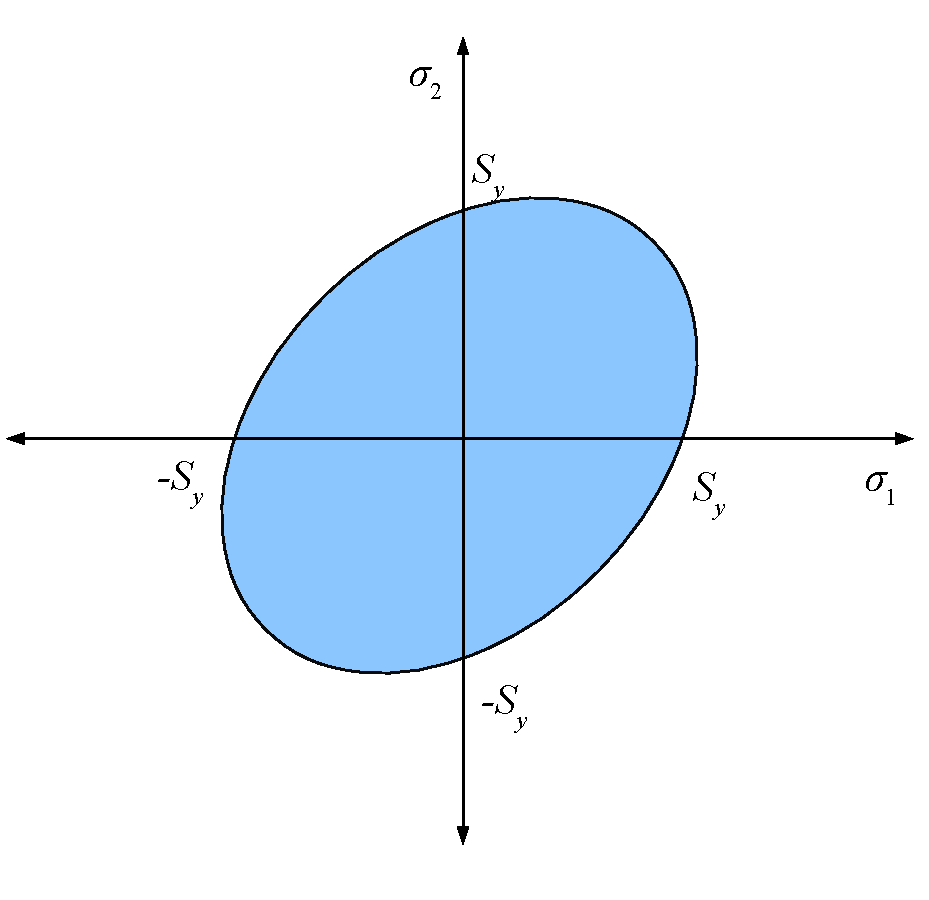
\includegraphics[scale=0.6]{pictures/Failure-theories/MDET-safe-zone}
  \caption{'Safe-zone' diagram for material under maximum distortion energy criterion.}
  \label{fig: MDET safe zone}
\end{marginfigure}

The safety factor according to the criterion can be written as

\begin{equation}
  N_s(MDET) = \frac{S_y}{\sigma_e}
\end{equation}

\begin{example} Failure of a ductile plane-stress element

  A plane stress element having $\sigma_x = 50a$ MPa, $\sigma_y = 30a$ MPa and $\tau_{xy} =  25a$ MPa. If under uniaxial test, the material fails when the normal stress is 70 MPa, determine the maximum the value a that will cause the material to fail if it follows

  \begin{figure}[H]
    \centering
    \begin{tikzpicture}[>=latex]
      \node [draw, fill=LightBlue!90, regular polygon, regular polygon sides=4, minimum width=2cm](A){};
      \draw [->,very thick] (A.north) --++ (90:1) node[above]{$\sigma_y = 30a$ MPa};
      \draw [->,very thick] (A.east) --++ (0:1) node[right]{$\sigma_x = 50a$ MPa};
      \draw [->,very thick] (A.west) --++ (180:1);
      \draw [->,very thick] (A.south) --++ (-90:1);
      \node at (A.north west) [yshift=2mm] (B){};
      \draw [-left to, very thick] (B) --++ (0:1.3);
      \node at (A.south east) [xshift=2mm] (C){};
      \draw [-right to, very thick] (C) --++ (90:1.3) node[above right]{$\tau_{xy} = 25a$ MPa};
      \node at (A.north west) [xshift=-2mm] (D){};
      \draw [-right to, very thick] (D) --++ (-90:1.3);
      \node at (A.south east) [yshift=-2mm] (E){};
      \draw [-left to, very thick] (E) --++ (180:1.3) ;
    \end{tikzpicture}
  \end{figure} 

    \begin{enumerate}
  \item Maximum shear stress criterion
  \item Maximum distortion energy criterion
  \end{enumerate}
\end{example}

\begin{solution}

  First, the uniaxial test indicates the material’s yield stress, which is 70 MPa. In either case, to determine the maximum a, we have to determine the element’s principal stresses

  \begin{align*}
      \sigma_{1,2} &= \frac{\sigma_x + \sigma_y}{2} \pm \sqrt {\left( \frac{\sigma_x - \sigma_y}{2} \right)^2 - \tau _{xy}^2}  \\ 
                   &= \frac{50a + 30a}{2} \pm \sqrt {\left( \frac{50a - 30a}{2} \right)^2 + (25a)^2}  \\ 
                   &= a\left[ 40 \pm \sqrt {10^2 + 25^2} \right] \\ 
                   &= 67a \text{, } 13a \\ 
  \end{align*}
  
  \begin{enumerate}
  \item For maximum shear stress criterion, since the two principal stresses are of the same signs, we know that the absolute maximum stress is out-of-plane equal to $\sigma_1/2$. We can apply equation so that
    
    \[\begin{gathered}
        \frac{\sigma_1}{2} = \frac{S_y}{2} \hfill \\
        67a = 70 \hfill \\
        a = 1.04 \hfill \\ 
      \end{gathered} \]
    
  \item For maximum distortion energy theory, we have that
    
    \[\begin{gathered}
        \sigma_1^2 -\sigma_1\sigma_2 + \sigma_2^2 = S_y^2 \\ 
        a^2 \left( 67^2 - (67)(13) + 13^2 \right) = (70)^2 \\ 
        3787a^2 = 4900 \\ 
        a = 1.14 \\ 
      \end{gathered} \]
    \end{enumerate}
\end{solution}

\subsection{Ductile Coulomb-Mohr theory}

Not all materials have the same compressive and tensile strengths. For example, the yield strengths of magnesium alloys in compression is approximately 50 percent of their yield strength in tension. The ultimate strength of grey cast irons in compression, on the other hand, can be as large as 300-400\% of their tensile strengths.

Mohr’s theory uses the results of three tests: tension, compression, and shear to construct three Mohr’s circles describing the state of stress at yield under the corresponding tests. Tangential lines connect the circles on the top and bottom of the circles to define a failure envelope of the theory.

A variation of Mohr’s theory, called the \emph{Coulomb-Mohr theory} or the \emph{internal-friction theory}, assume the tangential lines are straight. With this assumption, only the tensile and compressive strengths are necessary. Consider the conventional ordering of the principal stresses such that $\sigma_1 > \sigma_2 > \sigma_3$. The theory simply reduces to 

\[\frac{\sigma_1}{S_{ut}} - \frac{\sigma_3}{S_{uc}} = 1\]

For plane stress, when the two principal stresses $\sigma_A > \sigma_B > 0$, the failure condition become

\[\sigma_A > S_{ut}\]

When  $\sigma_A > 0 > \sigma_B$, the condition becomes

\[\frac{\sigma_A}{S_{ut}} - \frac{\sigma_B}{S_{uc}} > 1\]

When  $0 > \sigma_A > \sigma_B$, the condition becomes

\[\sigma_B <  - S_{uc}\]

\begin{marginfigure}
  \centering
  \begin{tikzpicture}[scale=0.5]
    \draw [fill=LightSkyBlue] (1.5,1.5) -- (1.5,0) node[below right]{$S_{ut}$}-- (0,-3) node[right]{$S_{uc}$}-- (-3,-3) -- (-3,0) node[below left]{$S_{uc}$} -- (0,1.5) node[above left]{$S_{ut}$} -- cycle;
    \draw [<->] (-5,0) --++ (0:8) node[right]{$\sigma_1$};
    \draw [<->] (0,-5) --++ (90:8) node[above]{$\sigma_2$};
  \end{tikzpicture}
 % 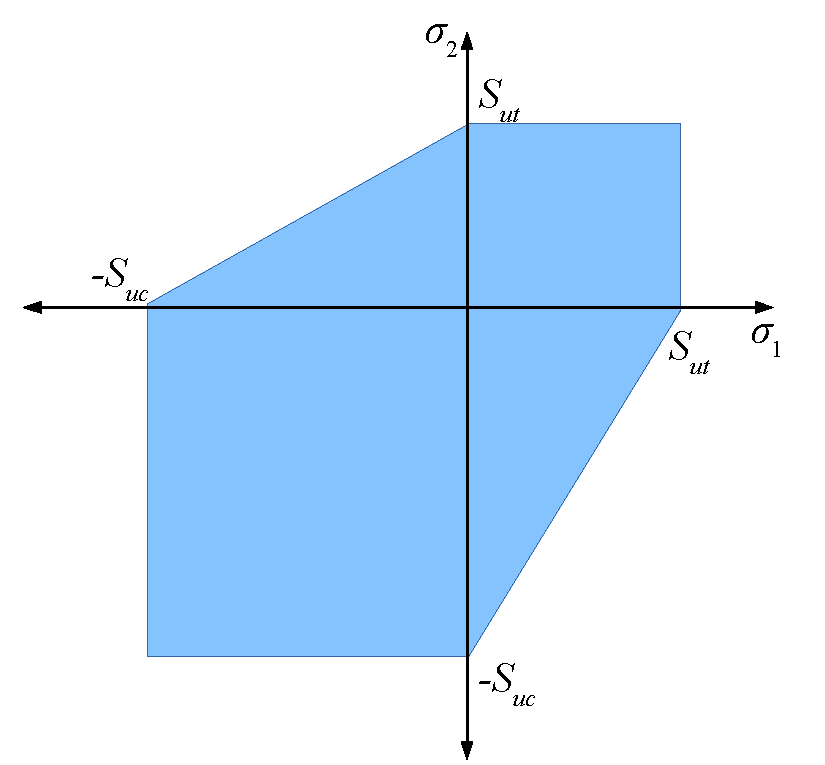
\includegraphics[scale=0.6]{pictures/Failure-theories/CM-ductile-safe-zone}
  \caption{`Safe-zone' diagram for material under ductile Coulomb-Mohr criterion.}
  \label{fig: Coulomb-Mohr ductile safe zone}
\end{marginfigure}

For design equations, incorporating the safety factor $N_s$, simply divide all strengths by the factor.

\begin{equation}
  \begin{array}{l l l}
  \sigma_A > \dfrac{S_{ut}}{N_s} & & \sigma_A > \sigma_B > 0 \\[10pt]
  \dfrac{\sigma_A}{S_{ut}} - \dfrac{\sigma_B}{S_{uc}} > \dfrac{1}{N_s} & & \sigma_A > 0 > \sigma_B \\[10pt]
    \sigma_B <  -\dfrac{S_{uc}}{N_s} & & \sigma_B < \sigma_A < 0
  \end{array}
\end{equation}

\subsection{Maximum principal stress theory}

Also called \emph{Rankine’s criterion} or \emph{maximum normal stress criterion}, it states that yielding begins at a point in a member where the maximum principal stress reaches a value equal to the tensile yield stress $S_{ut}$. For example, assume that a nonzero principal stress acts at a point in the member. According to this criterion, yielding will occur when $\sigma_1$ or $\sigma_2$ reaches the value $S_{ut}$. If the material is subjected to plane stress, we require that

\[\begin{gathered}
    \left| \sigma _1 \right| \leqslant S_{ut} \hfill \\
    \left| \sigma _2 \right| \leqslant S_{uc} \hfill \\ 
  \end{gathered} \]

These equations are shown graphically in \cref{fig: MNST safe zone}. It is seen that if the stress coordinate at a point in the material falls on the boundary or outside the shaded area, the material is said to fracture.

\begin{marginfigure}
  \centering
  \begin{tikzpicture}[scale=0.5]
    \node [draw, rectangle, xshift=-0.5cm, yshift=-0.5cm, fill=LightSkyBlue, minimum height=3cm, minimum width=3cm](sq){};
    \draw [<->] (-5,0) --++ (0:8) node[right]{$\sigma_1$};
    \node at (sq.east) [yshift=7mm, right] {$S_{ut}$};
    \node at (sq.west) [yshift=7mm, left] {$S_{uc}$};
    \node at (sq.north) [xshift=1cm, above] {$S_{ut}$};
    \node at (sq.south) [xshift=7mm, below] {$S_{uc}$};
    \draw [<->] (0,-5) --++ (90:8) node[above]{$\sigma_2$};
  \end{tikzpicture}
  % \includegraphics[scale=0.6]{pictures/Failure-theories/MNST-safe-zone}
  \caption{'Safe-zone' diagram for material under maximum principal stress criterion.}
  \label{fig: MNST safe zone}
\end{marginfigure}

Experimentally, the criterion has been found to be in close agreement with the behavior of brittle materials that have strain diagrams that are similar in both tension and compression. The safety factor according to the criterion can be expressed in design equations as

\begin{equation}
  \begin{array}{l l l}
  \sigma_1 > \dfrac{S_{ut}}{N_s} & & \sigma_1 > \sigma_2 > 0 \\
  \left. \hspace{-0.23cm}
  \begin{array}{l l l}
    \sigma_1 & > & \dfrac{S_{ut}}{N_s} \\
    \sigma_2 & < & -\dfrac{S_{uc}}{N_s}
    \end{array} \right\} & & \sigma_1 > 0 > \sigma_2 \\
    \sigma_2 <  - \dfrac{S_{uc}}{N_s} & & \sigma _2 < \sigma _1 < 0
  \end{array}
\end{equation}

\subsection{Modified Coulomb-Mohr theory}

Over the years, various empirical theories have been proposed to modify the basic failure theories. Coulomb-Mohr theory was proposed to predict fracture in brittle materials for which compressive strength is much greater than tensile strength. The failure condition is identical to that of ductile Coulomb-Mohr theory. However, there are still discrepancies between the condition and experimental results. The theory, consequently, is slightly modified to better accommodate the results.

The modified Coulomb-Mohr theory failure condition can be expressed as

\begin{equation}
  \begin{array}{ll}
    \sigma_1 < \dfrac{S_{ut}}{N_s} &
      \begin{gathered}
        \sigma_1 > \sigma_2 > 0 \hfill \\ 
        \sigma_1 > 0 \left| \dfrac{\sigma_2}{\sigma_1} \right| > 1 
      \end{gathered} \\[20pt]
    \dfrac{\sigma_1(S_{uc} - S_{ut})}{S_{uc}S_{ut}} - \dfrac{\sigma_2}{S_{uc}} > \dfrac{1}{N_s} & \sigma_1 > 0 > \sigma_2\text{ and }\left| \dfrac{\sigma_2}{\sigma_1} \right| < 1 \\[10pt]
    \sigma_2 <  -\dfrac{S_{uc}}{N_s} & \sigma_2 < \sigma_1 < 0
  \end{array}
\end{equation}

The failure condition diagram for the theory is illustrated in \cref{fig: MCM safe zone}

\begin{marginfigure}
  \centering
  \begin{tikzpicture}[scale=0.5]
    \draw [fill=LightSkyBlue] (1.5,1.5) -- (-1.5,1.5) -- (-4,0) -- (-4,-4) -- (0,-4) -- (1.5,-1.5) -- cycle;
    \node at (1.5,0) [below right]{$S_{ut}$};
    \node at (0,-4) [right]{$S_{uc}$};
    \node at (-4,0) [below left]{$S_{uc}$};
    \node at (0,1.5) [above right]{$S_{ut}$};
    \draw [<->] (-5.5,0) --++ (0:8) node[right]{$\sigma_1$};
    \draw [<->] (0,-5.5) --++ (90:8) node[above]{$\sigma_2$};
    \draw [dashed] (2,-2) -- (-2,2) node[left]{Shear diagonal};
  \end{tikzpicture}
  % 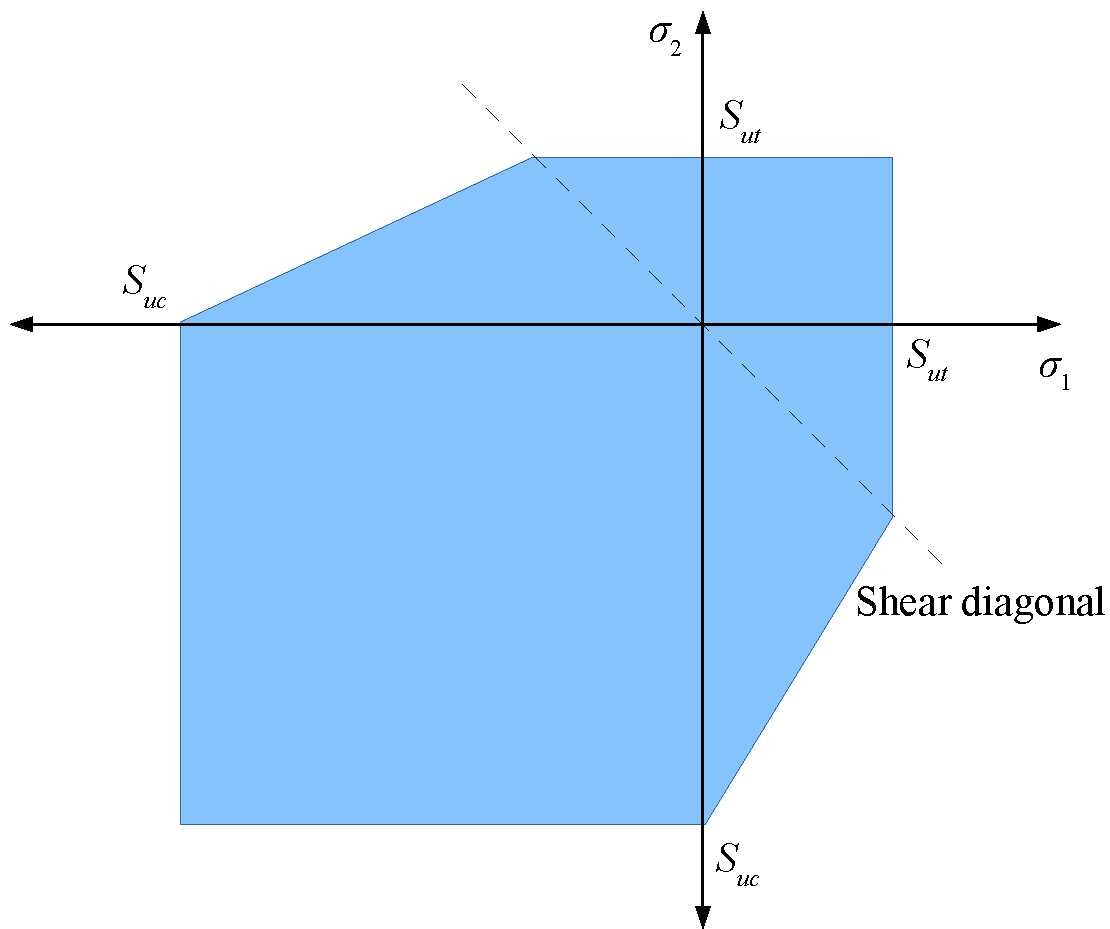
\includegraphics[scale=0.5]{pictures/Failure-theories/MCM-brittle-safe-zone}
  \caption{'Safe-zone' diagram for material under modified Coulomb-Mohr criterion.}
  \label{fig: MCM safe zone}
\end{marginfigure}

\subsection{Criterion selection}

With an exception of a few, most ductile materials have the same tensile and compressive yield strengths. Therefore, \emph{maximum distortion energy theory} should be applicable. It is also more convenient than other maximum shear stress theory in that one mathematical expression applies to all states of stress regardless of the signs of the principal stresses.
For brittle materials, \emph{modified Coulomb-Mohr theory} shows the best fit to most experimental results and should be applied.

\section{Fatigue} \label{section: fatigue failure}

Fatigue has been defined as “the progressive localized permanent structural change that occurs in a material subjected to repeated or fluctuating strains at stresses having a maximum value less than the tensile strength of the material” (ASM, 1975). Fracture of a structural member as a result of repeated cycles of load or fluctuating loads in commonly referred to as a fatigue fracture or fatigue failure. The corresponding number of load cycles or the time during which the member is subjected to these loads before fracture occurs is referred to as the fatigue life.

The type of fatigue failure can be categorized base on the number of cycles before failure, $N$: high cycle fatigue for $N > 10^7$ cycles and low cycle fatigue for $N < 10^7$ cycles. High cycle fatigue is characterized by small elastic strains and can be captured by stress-based parameters. Low cycle fatigue, on the other hand, is characterized by large plastic strains and is captured by strain-based parameters.

To simplify the problem of fatigue failure, we can assume that the repeated loading causes the internal stress in the material to take a sinusoidal form, i.e.

\begin{figure}[h]
  \centering
  \begin{tikzpicture}[>=latex]
    \draw[<->] (-5,0) -- (5,0) node[right] {$t$}; 
    \draw[<->] (0,-1) -- (0,2) node[above] {$\sigma$};
    \draw[color=blue, domain=-4:4, samples=100]   plot (\x,{sin(3.5*\x r)+0.5})    node[right] {$\sigma = {\sigma _a}\sin 2\pi ft + {\sigma _m}$}; 
  \end{tikzpicture}
\end{figure}

\[\sigma  = \sigma _a\sin 2\pi ft + \sigma _m\]

where $f$ is the frequency of the load, $\sigma_a$ is the stress amplitude, and $\sigma_m$ is the mean stress.
When testing for material fatigue, it is common to test for the relationship between the exerted stress and the number of cycles before the specimen fails. This \emph{endurance} graph or $S-N$ graph, normally shows that as the alternating stress amplitude increases, the number of cycle the material can take before failure decreases. Some materials exhibit endurance limits--lower limits of stress amplitudes under which the materials no longer exhibit fatigue fracture. For other materials that do not exhibit endurance limits, it is customary to define the stresses to cause failure under a given number of cycle, say $N = 10^7$, as the \emph{endurance limit} or \emph{fatigue strength}, $S_e$.

\begin{figure}[h]
  \centering
  \begin{tikzpicture}[>=latex]
    %grid
    \draw[ultra thin,color=lightgray] (0,0) grid (10,6);
    %axes
    \draw[<->]  (0,6) node [left] {$\sigma_a$} -- (0,5) node[left]{$S_l$} -- (0,2) node[left]{$S_e$}
    -- (0,0) node[below] {$10^3$} --
    (2,0)  node[below]{$10^4$} -- (4,0) node[below]{$10^5$} -- (6,0) node[below]{$10^6$} --
    (8,0) node[below]{$10^7$} -- (10,0) node[right] {$N$};
    % Steel
    \draw[very thick, blue] (0,5) to (3.5,3) to [out=-28,in=-180] (8,2) node[above]{Steel} to (10,2);
    \draw[very thick, green] (0,5) to [out=-40,in=160] (6.5,1) node[below left]{Aluminum} to (9,0);
  \end{tikzpicture}
  \caption{A typical endurance diagram showing stress amplitude $\sigma_a$ vs number of cycles to failure $N$.}
  \label{fig: S-N diagram}
\end{figure}

Typically, steel exhibit this endurance limit. However, many aluminum alloys do not; there does not exist a minimum stress below which fatigue does not occur. This is why these aluminum alloys, though lighter, simply cannot replace steel in many machine design applications.

\subsection{Fatigue under zero mean stress}

When the load is completely reversed, resulting in zero mean stress ($\sigma_m = 0$), fatigue failure can mostly be described by stress amplitude. At the lower end of this spectrum where the number of cycles to failure $N = 10^3$, the stress amplitude that leads to failure is called the \emph{low cycle fatigue limit}, $S_l$, and can be approximated as

\begin{equation}
  S_l = \left\{
    \renewcommand{\arraystretch}{1.2}
    \begin{array}{ll}
      0.9 S_{ut} &\text{ for bending} \\
      0.75 S_{ut} &\text{ for axial} \\
      0.72 S_{ut} &\text{ for torsion}
    \end{array}
  \right.
\end{equation}

On the far end of the spectrum where $N = 10^7$, the stress amplitude is the \emph{endurance limit}, $S_e$, which can be approximated as

\begin{equation}
  S_e = \left\{
    \renewcommand{\arraystretch}{1.2}
    \begin{array}{ll}
      0.5 S_{ut} & \text{ for bending} \\
      0.45 S_{ut} &\text{ for axial} \\
      0.29 S_{ut} &\text{ for torsion}
    \end{array}
  \right.
\end{equation}

For stress amplitude between the two ends, the expected number of cycles, $N$, can be interpolated. The relationship between them can be written as

\begin{equation}
  \sigma_a = 10^cN^b
\end{equation}

where $c$ and $b$ are parameters that can be obtained from

\begin{align*}
  b &= - \frac{1}{3} \log \dfrac{S_l}{S_e} \\
  c &= \log \dfrac{S_l^2}{S_e}
\end{align*}

Parameter $b$ is between $-0.06$ to $-0.14$ for most metals.

\subsection{Fatigue under nonzero mean stress}

Nonzero mean stresses have a significant effect on the fatigue strength of a material. There have been several relations proposed to describe the effects of mean stress. Three of such relations are

\begin{enumerate}
\item Soderberg relation
  \begin{equation}
    \frac{\sigma_a}{S_e} + \frac{\sigma _m}{S_y} = \frac{1}{N_s}
  \end{equation}
\item Gerber relation
  \begin{equation}
    \frac{\sigma_a}{S_e} + \left( \frac{\sigma_m}{S_{ut}} \right)^2 = \frac{1}{N_s}
  \end{equation}
\item Goodman relation
  \begin{equation}
    \frac{\sigma_a}{S_e} + \frac{\sigma _m}{S_{ut}} = \frac{1}{N_s}
  \end{equation}
\end{enumerate}

where $\sigma_a$ is the stress amplitude, $S_e$ is the endurance limit, $S_y$ is the yield stress, $\sigma_m$ is the mean stress, and $S_{ut}$ is the ultimate tensile strength. For most metals, the Soderberg relation yields conservative estimates of critical stress amplitude. The Goodman relation gives reasonably good results for brittle materials, whereas it is conservative for ductile materials. The Gerber relation yields fairly good estimates for stress amplitude for ductile materials.

Each relation can be expressed as a line on which all combinations of stress amplitude and average stress result in the same number of cycle to failure, also called \emph{constant life line}.

\begin{figure}[h]
  \centering
  \begin{tikzpicture}[>=latex]
    \begin{axis} [
      height=0.4\textwidth,
      width=0.7\textwidth,
      xlabel={Average Stress $\sigma_m$},
      ylabel={Stress Amplitude $\sigma_a$},
      xmin=0, xmax=500,
      xtick={300, 450},
      xticklabels={$S_y$, $S_{ut}$},
      ymin=0, ymax=250,
      ytick={225},
      yticklabels={$S_e$},
      domain=0:450,
      axis x line=bottom,
      axis y line=left,
      ]
      % N_s = 1, S_e = 225, S_y = 300, S_ut = 450
      \addplot+[mark=none, domain=0:300]{-225/300*x + 225} node[midway, below, rotate=-37]{Soderberg};
      \addplot+[mark=none, dashdotted]{-225/450*x + 225} node[midway, below, rotate=-25]{Goodman};
      \addplot+[mark=none, dashed]{-225*(x/450)^2 + 225} node[midway, below, rotate=-30]{Gerber};
    \end{axis}
  \end{tikzpicture}
  \caption{Constant life lines for various nonzero mean stress relations with
    $N_s$ = 1}
  \label{fig: nonzero mean stress relations}
\end{figure}

\begin{example} Fatigue failure of a rod under a periodic tensile load

  A cylindrical rod shall operate under a periodic tensile load as shown in the graph. Material of the rod is AISI1050 which has the following properties.
  Yield strength = 427 MPa
  Ultimate tensile strength = 748 MPa
  Modified endurance limit = 300 MPa
  Determine the suitable diameter of the rod. Use Soderberg line with $N_s$ = 3

  \begin{figure}[H]
    \centering
    % 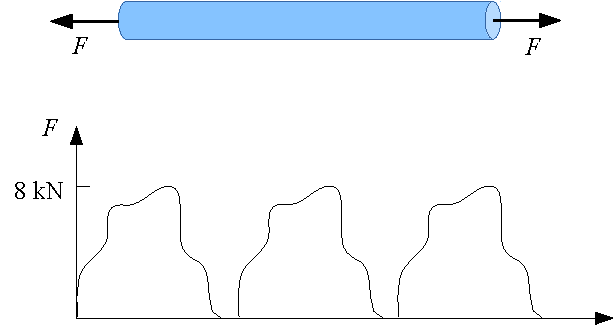
\includegraphics[scale=0.9]{pictures/Failure-theories/fatigue-example}
    \begin{tikzpicture}
      \node[draw, cylinder, minimum height=6cm, minimum width=5mm, inner sep=4](beam){};
      \draw [->, very thick] (beam.east) ++ (180:0.15) --++ (0:1) node[below]{$F$};
      \draw [->, very thick] (beam.west) --++ (180:1) node[below]{$F$};
    \end{tikzpicture} \\[10pt]
    \begin{tikzpicture}
      \begin{axis} [
        ymin=0,ymax=8000,
        ylabel={$F$},
        xlabel={time (s)},
        xmin=0,
        height=0.4\textwidth,
        ]
        \addplot [semithick, samples=100, domain=0:10.8] {abs(8000*sin(50*\x))};
      \end{axis}
    \end{tikzpicture}
  \end{figure}
\end{example}
\begin{solution}
    The safety factor of a member under alternate loading using the Soderberg line is as follows

    \[\frac{\sigma_a}{S_e} + \frac{\sigma_m}{S_y} = \frac{1}{N_s}\]

  The stress amplitude is simply the force amplitude divided by the cross sectional area of the rod.

  \[\sigma_a = \frac{(8000 + 0)/2}{\dfrac{\pi }{4}d^2} = \frac{16000}{\pi d^2}\]

  According to the Soderberg relation, we have

  \begin{gather*}
    \frac{\sigma_m}{S_y} + \frac{\sigma _a}{S_e} = \frac{1}{3} \\ 
    \dfrac{\dfrac{4000}{\dfrac{\pi }{4}d^2}}{427 \times 10^6} + \dfrac{\dfrac{16000}{\pi d^2}}{300 \times 10^6} = \frac{1}{3} \\[1em] 
    d^2 = 6.29 \times 10^{-5} \hfill \\
    d = 7.9 \times 10^{-3} = 7.9 \text{ mm} \hfill \\ 
  \end{gather*}
  Therefore, the rod’s diameter must be 7.9 mm.
\end{solution}

\section{Buckling} \label{section: buckling}

Whenever a member is designed, it is necessary that it satisfy specific strength, deflection, and stability requirements. In the previous chapters we have discussed some of the methods used to determine the member’s strength and deflection, while assuming that the member was always in stable equilibrium. Some members, however, may be subjected to compressive loads, which, if sufficiently large, can cause the member to deflect laterally. To be more specific, long slender members subjected to an axial compressive force are called columns, and the lateral deflection that occurs is called buckling. Buckling of a column can lead to a sudden and often disastrous failure of a structure or mechanism, and therefore special attention must be given to the design of columns to prevent such problems.

The maximum axial load that a column can support is called the critical load, $P_{cr}$. Any additional loading will cause the column to buckle and therefore deflect laterally. Depending on the supports of a column, the critical load can vary.

\subsection{Ideal column with pin supports}

In this section we will determine the critical buckling load for a column that is pin-supported. The column to be considered is an \emph{ideal column}, meaning one that is perfectly straight before loading, is made of homogeneous material, and upon which the load is applied through the centroid of the cross section.
When the critical load $P_{cr}$ is reached, the column is on the verge of becoming unstable, so that a small lateral force $F$ will cause the column to remain in the deflected position when $F$ is removed. Any slight reduction in the load $P$ from Pcr will allow the column to straighten out, and any slight increase in $P$ beyond $P_{cr}$ will cause further increases in lateral deflection.
Whether or not a column will remain stable or become unstable when subjected to an axial load will depend on its ability to restore itself, which is based on its resistance to bending. Therefore, to determine the critical load and the buckled shape of the column, we will apply the equation for beam bending,

\[EI\frac{d^2v}{dx^2} = M\]

Recall that this equation assumes that the slope of the curve is small and that deflections occur only by bending. When the column is in its deflected position, the internal bending moment can be determined by using the method of sections. The bending moment in the beam is simply the product of the compressive load $P$ and the maximum deflection in the middle $v$. Note that the bending moment is negative, according to the sign convention used to establish equation so that $M = –Pv$. Thus equation becomes

  \begin{figure}[H]
    \centering
    \begin{tikzpicture}[>=latex]
      % beam and neutral axis
      \draw [LightBlue!90, line width=10pt] (-4,0) node(A){} arc (110:70:14) node(B){};
      \draw [dashed] (-4,0) arc (110:70:14);
      % left support
      \node at (A.center) [anchor=east, draw, regular polygon, regular polygon sides=3, minimum height=4mm, inner sep=0, fill=LightGrey, shape border rotate=30](C){};
      \node at (A.center) [draw, circle, inner sep=1.5, fill=LightGrey]{};
      % right support
      \node at (B.center) [anchor=west, draw, regular polygon, regular polygon sides=3, minimum height=4mm, inner sep=0, fill=LightGrey, shape border rotate=-30](D){};
      \node at (B.center) [draw, circle, inner sep=1.5, fill=LightGrey]{};
      % wall
      \node at (D.east) [anchor=west,rectangle, pattern=north east lines, minimum height=2cm, minimum width=0.5cm]{};
      % force
      \draw [<-, line width=2pt] (C.west) -- ++ (180:1) node[left]{$P$};
      % horizontal level
      \draw [dashed] (A.center) -- (B.center);
      % vertical deflection
      \draw [<->] (A.center) ++ (3,0) --++ (90:0.75) node[midway, right]{$v$};
    \end{tikzpicture}
  \end{figure}
  
  \begin{gather*}
    EI\frac{d^2v}{dx^2} =  - Pv \\
    \frac{d^2v}{dx^2} + \left( \frac{P}{EI} \right)v = 0 
  \end{gather*}

This is a homogeneous second order linear differential equation with constant coefficients. The solution is of the form

\begin{equation} \label{eqn: gen solution}
  v = C_1\sin \left( \sqrt {\frac{P}{EI} x} \right) + C_2\cos \left( \sqrt {\frac{P}{EI}} x \right)
\end{equation}

Using the two boundary conditions that $v(x = 0) = 0$ and $v(x = L) = 0$, it can be determined that $C_2 = 0$ and

\[C_1\sin \left( \sqrt {\frac{P}{EI}} L \right) = 0\]

One way for this solution to be valid is for $C_1 = 0$, but this means that the column will remain straight since it leads to $v = 0$. This is a trivial solution and is not particularly interesting. The other, more interesting possibility is for 

\[\sin \left( \sqrt {\frac{P}{EI}} L \right) = 0\]

which is satisfied if

\begin{equation} \label{eqn: mode shape sub}
  \sqrt {\frac{P}{EI}} L = n\pi
\end{equation}

or

\begin{equation}
  P = \frac{n^2\pi^2EI}{L^2} \hspace{1cm}n = 1,2,3,...
\end{equation}

The smallest value of $P_{cr}$ is obtained when $n = 1$, so the \emph{critical load} for the column is therefore

\begin{equation}
  P_{cr} = \frac{\pi ^2EI}{L^2}
\end{equation}

This load is sometimes referred to as the \emph{Euler load}.

For the corresponding buckling mode shapes, substitute the expression in equation \cref{eqn: mode shape sub} into \cref{eqn: gen solution} along with other solved parameters, we have

\[v = C_2\sin \frac{n\pi x}{L}\]

Let us explore other buckling loads and their corresponding mode shapes. For $n = 2$, we have

$$ P = \frac{4 \pi^2 E I}{L^2} $$

and the mode shape is described by

$$ v = C_2 \sin \frac{2 \pi x}{L} $$

\begin{figure}[H]
  \centering
  \begin{tikzpicture}[>=latex]
    % beam and neutral axis
    \draw [LightBlue!90, line width=10pt, smooth, domain=0:10] node(A){} plot (\x, {sin(2*pi*\x/10 r)}) node(B){};
    % \draw [dashed] (-4,0) arc (110:70:14);
    % left support
    \node at (A.center) [anchor=east, draw, regular polygon, regular polygon sides=3, minimum height=4mm, inner sep=0, fill=LightGrey, shape border rotate=30](C){};
    \node at (A.center) [draw, circle, inner sep=1.5, fill=LightGrey]{};
    % right support
    \node at (B.center) [anchor=west, draw, regular polygon, regular polygon sides=3, minimum height=4mm, inner sep=0, fill=LightGrey, shape border rotate=-30](D){};
    \node at (B.center) [draw, circle, inner sep=1.5, fill=LightGrey]{};
    % wall
    \node at (D.east) [anchor=west,rectangle, pattern=north east lines, minimum height=2cm, minimum width=0.5cm]{};
    % force
    \draw [<-, line width=2pt] (C.west) -- ++ (180:1) node[left]{$P$};
    % horizontal level
    \draw [dashed] (A.center) -- (B.center);
  \end{tikzpicture}
\end{figure}
  
And for $n=3$, the buckling load and corresponding mode shape are

$$ P = \frac{4 \pi^2 E I}{L^2} $$

$$ v = C_2 \sin \frac{2 \pi x}{L} $$
  
\begin{figure}[H]
  \centering
  \begin{tikzpicture}[>=latex]
    % beam and neutral axis
    \draw [LightBlue!90, line width=10pt, smooth, domain=0:10] node(A){} plot (\x, {sin(3*pi*\x/10 r)}) node(B){};
    % \draw [dashed] (-4,0) arc (110:70:14);
    % left support
    \node at (A.center) [anchor=east, draw, regular polygon, regular polygon sides=3, minimum height=4mm, inner sep=0, fill=LightGrey, shape border rotate=30](C){};
    \node at (A.center) [draw, circle, inner sep=1.5, fill=LightGrey]{};
    % right support
    \node at (B.center) [anchor=west, draw, regular polygon, regular polygon sides=3, minimum height=4mm, inner sep=0, fill=LightGrey, shape border rotate=-30](D){};
    \node at (B.center) [draw, circle, inner sep=1.5, fill=LightGrey]{};
    % wall
    \node at (D.east) [anchor=west,rectangle, pattern=north east lines, minimum height=2cm, minimum width=0.5cm]{};
    % force
    \draw [<-, line width=2pt] (C.west) -- ++ (180:1) node[left]{$P$};
    % horizontal level
    \draw [dashed] (A.center) -- (B.center);
  \end{tikzpicture}
\end{figure}

For purposes of design, the critical load equation can also be written in a more useful form by expressing $I = Ar_g^2$, where $A$ is the cross-sectional area and $r_g$ is the \emph{radius of gyration} of the cross-sectional area. Thus,

\begin{align*}
  P_{cr} &= \frac{\pi^2EAr_g^2}{L^2} \\ 
  \frac{P_{cr}}{A} &= \frac{\pi ^2E}{(L/r_g)^2}
\end{align*}

or

\begin{equation}
  \sigma_{cr} = \frac{\pi ^2E}{(L/r_g)^2}
\end{equation}

The geometric ratio $L/r_g$ is known as the \emph{slenderness ratio}. It is a measure of the column’s flexibility.

\subsection{Columns having various types of supports}

In some other cases where the columns are supported in some other way, so that the column’s ends may be restricted against rotations or deflection in different ways, determination of the buckling load on the column follows the same procedure. Take, for example, a column whose one end is fixed while the other is free. Assume that the compressive load is exerted onto the free end. The internal bending moment at an arbitrary section, whose lateral deflection is $v$, is $M = P(\delta – v)$. The differential equation for the deflection curve is

  \begin{figure}[H]
    \centering
    \begin{tikzpicture}[>=latex]
      % beam and neutral axis
      \draw [LightBlue!90, line width=10pt] (-4,0) node(A){} arc (-110:-90:28) node[inner sep=0pt](B){};
      \draw [dashed] (-4,0) arc (-110:-90:28);
      % wall
      \node at (B.west) [anchor=west,rectangle, pattern=north east lines, minimum height=2cm, minimum width=0.5cm]{};
      % force
      \draw [<-, line width=2pt] (A.center) -- ++ (180:1) node[left]{$P$};
      % horizontal level
      \draw [dashed] (B.center) -- ++ (180:10);
      % vertical deflection and max deflection
      \draw [<->] (A.center)  --++ (-90:1.7) node[midway, right]{$\delta$};
      \draw [<->] (B.center)  ++ (-6.4,0) --++ (90:0.8) node[midway, right]{$v$};
    \end{tikzpicture}
  \end{figure}

\begin{gather*}
  EI\frac{d^2v}{dx^2} = P(\delta  - v) \\ 
  \frac{d^2v}{dx^2} + \frac{P}{EI}v = \frac{P}{EI}\delta  \\ 
\end{gather*}

Since this equation is nonhomogeneous, the solution consists of both a complementary and particular solutions.

\[v = C_1\sin \left( \sqrt {\frac{P}{EI}} x \right) + C_2\cos \left( \sqrt {\frac{P}{EI}} x \right) + \delta \]

Solving for constants of integration using $v(x = 0) = 0$ we have that 

\begin{equation*}
  C_2 = -\delta
\end{equation*}

At the fixed end $v'(x=0) = 0$

\begin{equation*}
  C_1 = 0
\end{equation*}

Finally, at the free end, the deflection is $\delta$, giving us

\[\delta \cos \left( \sqrt {\frac{P}{EI}} L \right) = 0\]

The nontrivial solution indicates that

\begin{gather*}
  \cos \left( \sqrt {\frac{P}{EI}} L \right) = 0 \\
  \sqrt {\frac{P}{EI}} L = \frac{(2n - 1)\pi }{2} \hspace{1cm} n = 1, 2, 3, \ldots
\end{gather*}

The smallest critical load ($n = 0$) is

\begin{equation}
  P_{cr} = \frac{\pi^2EI}{4L^2}
\end{equation}

By comparison, this critical load is a quarter of the critical load of a pin-supported column. Similar derivations can be used to determine the critical loads of those columns whose supports are different from the ones already given. For the case of a column having ends that are pinned or free to rotate, $L$ represents the unsupported distance between the points of zero moment. For other types of supports, the column’s \emph{effective length}, $L_e$, can be used to represent that length and substituted into the critical load equation so that

\begin{equation} \label{eqn: Euler's formula}
\begin{gathered}
  P_{cr} = \frac{\pi^2EI}{L_e^2} = \frac{\pi ^2EI}{(KL)^2} \hfill \\
  \sigma_{cr} = \frac{\pi ^2E}{(KL/r_g)^2} \hfill \\ 
\end{gathered}
\end{equation}

where $L_e = KL$ in which $K$ is the \emph{effective-length factor} and $KL/r_g$ is the \emph{effective-slenderness ratio}. The table of $K$ values for various end supports is given below.

\begin{table}[h]
  \centering
  \caption{Effective length factor ($K$) value for beam under various support conditions}
  {\renewcommand{\arraystretch}{1.2}
  \begin{tabular}{ lc }
    \toprule
    End Support & $K$ value \\
    \midrule
    Pinned ends & 1 \\
    Fixed and free ends & 2 \\
    Fixed ends & 0.5 \\
    Pinned and fixed ends & 0.7 \\
    \bottomrule
  \end{tabular}}
\end{table}

\begin{example}
  Before the development of proper installation technique, train track buckling problems due to thermal loads plague continuous welded rails (CWR). Let us assume that a section of a welded rail is 10 m long and its cross-sectional moment of inertia and area are 400 cm$^4$ and 73 cm$^2$. The rail is made of steel with $\alpha = 12 \times 10^-6$ C$^{-1}$ and $E = 210$ GPa. Determine the change in temperature that will lead to buckling.

  \begin{figure}[H]
    \centering
    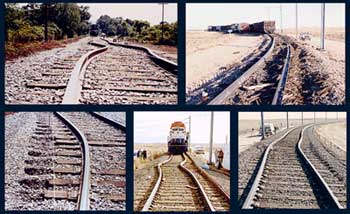
\includegraphics[scale=0.7]{pictures/Failure-theories/Rail_buckle}
    \caption{Train track buckling. (US Department of Transportation)}
  \end{figure}
\end{example}
\begin{solution}

  Buckling due to thermal load is a combination between two problems: buckling and thermal loading. Assuming that rail buckling happens on a first mode ($n = 1$), we have that

  \begin{align*}
    P_{cr} &= \frac{ \pi^2 EI }{ L^2 } 
  \end{align*}

  Now we need to determine the change in temperature that will lead to that critical load. Let points A and B be the two ends of the rail. Following steps to solve a statically indeterminate problem (equilibrium equation, compabitility equation, and Hooke's law), we can write that:

  \begin{align*}
    F_A = F_B = F
  \end{align*}

  Since the two ends of the rail are supported, its length cannot change, i.e. the changes in length due to support force and thermal change must cancel out.

  \begin{align*}
    &\delta_{AB} = 0 \\
    &\delta_T + \delta_F = 0
  \end{align*}

  Applying Hooke's law and thermal elongation to the equation, we can solve for the support force $F$

  \begin{align*}
    &\alpha \Delta T L + \frac {FL}{AE} = 0 \\
    &F = -\alpha \Delta T A E
  \end{align*}

  Finally, we know that the support force $F$ must be equal to the critical load $P_{cr}$ to cause buckling. We must, however, flip the sign of $F$ because $F > 0$ is tensile load while $P_{cr}$ is always compressive.

  \begin{align*}
    -F &= P_{cr} \\
    \alpha \Delta T A E &= \frac{ \pi^2 EI }{ L^2 } \\
    \Delta T &= \frac{ \pi^2 I }{ \alpha A L^2} = \frac{1}{\alpha} \left( \frac{ \pi r_g }{L} \right)^2 \\
       &= \frac{ \pi^2 (400 \times 10^{-8}) }{ (12 \times 10^{-6})(73 \times 10^{-4})(10^2)}\\
       &= 4.51\degree \text{ C}
  \end{align*}

  As we can see it requires very slight temperature change to cause buckling. However, with a proper installation technique called \emph{rail stressing}, the rail is pre-stretched before installation. This technique preloads the rail in tension and thus it will be much considerably less likely to buckle.
\end{solution}

\section*{Summary}

In this chapter, we study various ways engineering materials can fail. The first two, yield/fracture and fatigue are due to damage inflicted to the material by stress. Buckling, on the other hand, is due to the geometric instability of the structure brought upon by external compressive loads.

For yield and fracture, failure is due to static load. Yield occurs usually in ductile materials, while fracture occurs in brittle materials. The criteria introduced can be used to determine ‘equivalent’ stress to determine whether yield or fracture will occur in case of multiaxial stress.

Fatigue is due to repeated or periodic loading. The size of the load itself is not sufficiently large to cause yield or fracture to the material immediately, but after several cycles, the cumulative damage can cause failure. We have derived equations relative the stress amplitude to the number of cycles before failure, which also depends on material properties and whether the average stress is zero.

Buckling occurs because the internal bending moment in the beam is not enough to counter the external bending moment caused by the axial compressive load if a slight lateral perturbation occurs. The critical axial load depends on the dimensions of the body, material properties, and support conditions.

\section*{Exercises}

\begin{exercises}
  
  \item A plane stress element is under the following state of stress.  $\sigma_x = 150$ MPa, $\sigma_y = -200$ MPa , and $\tau_{xy} = 100$ MPa. The material has $S_y$ = 200 MPa, $S_{ut}$ = 250 MPa, and $S_{uc}$ = 300 MPa. Determine the safety factor under the following criteria.
  \begin{enumerate}
  \item MNST
  \item MSST
  \item MDET
  \item Modified Mohr-Coulomb theory
  \end{enumerate}

  \begin{figure}[H]
    \centering
    \begin{tikzpicture}
      \node [draw, fill=LightBlue!90, regular polygon, regular polygon sides=4, minimum width=2cm](A){};
      \draw [<-,very thick] (A.north) --++ (90:1) node[above]{$\sigma_y$ = -20 MPa};
      \draw [->,very thick] (A.east) --++ (0:1) node[right]{$\sigma_x$ = 150 MPa};
      \draw [->,very thick] (A.west) --++ (180:1);
      \draw [<-,very thick] (A.south) --++ (-90:1);
      \node at (A.north west) [yshift=2mm] (B){};
      \draw [-left to, very thick] (B) --++ (0:1.3);
      \node at (A.south east) [xshift=2mm] (C){};
      \draw [-right to, very thick] (C) --++ (90:1.3) node[above right]{$\tau_{xy}$ = 100 MPa};
      \node at (A.north west) [xshift=-2mm] (D){};
      \draw [-right to, very thick] (D) --++ (-90:1.3);
      \node at (A.south east) [yshift=-2mm] (E){};
      \draw [-left to, very thick] (E) --++ (180:1.3) ;
    \end{tikzpicture}
  \end{figure}
  
  \item A 2-m long, pinned-support prismatic steel ($E$ = 210 GPa) column is restrained in the middle. Its cross-sectional area is a circle with radius of 5 cm. Determine the safety factor of the column if it is compressed by the load of 700 N.

  \begin{figure}[H]
    \centering
    \begin{tikzpicture}
      \node at (0,0) [anchor=south, draw, rectangle, minimum height=0.4cm, minimum width=8cm,fill=LightBlue!90](A){};
      \node at (A.west) [anchor=east, draw, regular polygon, regular polygon sides=3, minimum height=4mm, inner sep=0, fill=LightGrey, shape border rotate=30](C){};
      \node at (A.west) [draw, circle, inner sep=1.5, fill=LightGrey]{};
      \node at (A.east) [anchor=west, draw, regular polygon, regular polygon sides=3, minimum height=4mm, inner sep=0, fill=LightGrey, shape border rotate=-30](B){};
      \node at (A.east) [draw, circle, inner sep=1.5, fill=LightGrey]{};
      \node at (B.east) [anchor=west,rectangle, pattern=north east lines, minimum height=2cm, minimum width=0.5cm]{};
      \draw [<-, line width=2pt] (C.west) -- ++ (180:1) node[left]{$P$ = 700 N};
      \node at (A.north) [anchor=south, draw, regular polygon, regular polygon sides=3, minimum height=4mm, inner sep=0, fill=LightGrey, shape border rotate=60]{};
      \node at (A.north) [draw, circle, inner sep=1.5, fill=LightGrey]{};
      \node at (A.south) [anchor=north, draw, regular polygon, regular polygon sides=3, minimum height=4mm, inner sep=0, fill=LightGrey, shape border rotate=0]{};
      \node at (A.south) [draw, circle, inner sep=1.5, fill=LightGrey]{};
      \node at (A.south west) [yshift=-0.8cm](D){};
      \node at (A.south east) [yshift=-0.8cm](E){};
      \draw [|<->|] (D) -- (E) node[midway, below]{2 m};
    \end{tikzpicture}
  \end{figure}
  
  \item A shaft made of AISI 1020 ($E$ = 210 GPa, $S_y$ = 400 MPa, and $S_{ut}$ = 600 MPa) is twisted back and forth by the torque of $T$ = [-200, 200] Nm. Size the proper shaft so that its safety factor is 3.

  \begin{figure}[H]
    \centering
    \begin{tikzpicture}
      \node at (0,0) [draw, cylinder, inner sep=5, minimum height=8cm, minimum width=1cm, fill=LightBlue!90](A){};
      \draw [->>, ultra thick] (A.east) ++ (180:5pt) --++(0:1) node[right]{$T$};
      \draw [->>, ultra thick] (A.west) --++(180:1) node[left]{$T$};
    \end{tikzpicture}
  \end{figure}

  \item You want to design a cylindrical beer can with 3 cm radius that contains a nice cold beer under 20 kPa pressure using the smallest possible thickness $t_1$. After you submitted the design to your manager, however, he told you to revise the design because when beer is shaken, it releases $\text{CO}_2$ that pressurizes the can to 60 kPa, using the smallest possible thickness $t_2$ but keeping the same 3 cm radius. If the aluminum used to manufacture the cans has a yield stress of 100 MPa, what is the difference in thickness between your second design and your first design $t_2 - t_1$? Note: use maximum distortion energy theory to determine failure.

    \begin{figure}[H]
    \centering
    \begin{tikzpicture}
      \node at (0,0) [draw, cylinder, inner sep=10, minimum height=4cm, minimum width=3cm, rotate=90, fill=LightBlue!90, fill opacity=0.5](E){};
      \node at (E.west) [draw, ellipse, dashed, minimum height=0.5cm, minimum width=2.8cm, yshift=10]{};
      \node at (5,0) [draw, circle, fill=LightBlue!90, inner sep=1cm](A){};
      \node at (5,0) [draw, circle, fill=White, inner sep=0.9cm](B){};
      \node at (A.west) [yshift=1.5cm](C){};
      \node at (A.east) [yshift=1.5cm](D){};
      \draw [|<->|] (C) -- (D) node[midway,above]{3 cm};
      \draw [|<-] (A.west) -- ++ (180:0.5) node[left]{$t$};
      \draw [|<-] (B.west) -- ++ (0:0.5);
    \end{tikzpicture}
  \end{figure}
  
  \item Assume that a state of triaxial principal stresses develops on an element as shown in the figure below. These stresses are directly proportional to a parameter a. If the yield stress in uniaxial stress is 250 MPa. What should a be in order for the element to start to yield based on the maximum distortional energy theory?

  \item A bar with a 20-mm diameter is being loaded axially by a periodic force of range $[3P, -P]$ until it is broken after $10^5$ cycles. The bar material has $S_y$ = 400 MPa, $S_{ut}$ = 550 MPa, and follows stress-fatigue life response curve.
  \[ \sigma_a = 10^{7.5}N^{-0.06} \]
  and its nonzero mean stress follows Gerber relation.
  \begin{enumerate}
  \item What is the load $P$?
  \item How many cycles does it take to break the same bar if the load if the load is changed to $[5P, 0]$
  \end{enumerate}
  
  \item A slender bar AB with pinned ends (simple supports) and length $L$ is held between immovable supports. What increase $\Delta T$ in the temperature of the bar will produce buckling at the Euler load?

  \item A circular bar of radius 1 cm and length 50 cm is fixed between two walls 50 cm apart. The bar is made of a material that has thermal coefficient of expansion $\alpha$ = 1.1x10$^{-6}$ / C and modulus of elasticity $E$ = 210 GPa and ultimate tensile stress $S_{ut}$ = 240 MPa. The material follows stress-fatigue life curve with zero mean stress of
  \[ \sigma_a = 10^{6.5}N^{-0.07} \]
  and the effect of nonzero mean stress follows Goodman relation so that
  \[ \frac{\sigma_a}{S_e} + \frac{\sigma_m}{S_{ut}} = 1 \]
  \begin{enumerate}
  \item If the initial bar temperature is $T$, what is the change in temperature $\Delta T$ required so that when the temperature is varied between $[T+\Delta T, T]$, the material would break due to fatigue after $10^6$ cycles?
  \item What is the change in temperature that will cause the bar to buckle?
  \end{enumerate}

  \item A 3-m long springboard at a water park is used repeatedly everyday by thousands of people. Assume that the average weight of a person using the board is 700 N, which keeps getting on and jumping off repeatedly. The board is made of AISI 1040 steel (a ductile material with $E$ = 210 GPa, $S_y$ = 415 MPa, and
  $S_{ut}$ = 620 MPa) and has a constant rectangular cross section with base width of 50 cm. Determine
  \begin{enumerate}
  \item the critical point of the springboard. (Hint: again, be specific.) Explain your reasoning.
  \item the required thickness $h$ of the board so it is safe under static loading. (A maximum constant load of 700 N.)
  \item the required thickness $h$ of the board so that it is safe under repeated loading. (Range of load between 0 and 700 N.) Use Soderberg relation to predict fatigue behavior with safety factor
    $N_s$ = 1.
  \end{enumerate}

\begin{pycode}
hp = random.randint(4,11)*5 # 20 - 55 hp
rpm = random.randint(3,8)*5*100 # 1500 - 4000 rpm
S_y = random.randint(2,8)*10*1e6 # 20 - 80 MPa
\end{pycode}

  \item An aluminum alloy ($S_{y}$ = \py{round(S_y/1e6)} MPa) is to be used for a drive shaft such that it transmits \py{hp} hp at \py{rpm} rpm. Determine the smallest diameter shaft that can be selected based on:
        \begin{enumerate}
          \item MDET
          \item MSST
        \end{enumerate}

\begin{pycode}
S_y = random.randint(2,5)*10*1e6 # 20-50 MPa
S_ut = S_y*1.5
E = random.randint(10,20)*10*1e9 # 100 - 200 GPa
dim = random.choice(['length','thickness'])
dim_num = round(random.randint(15,30)/10,1) if dim == 'length' else round(random.randint(5,15)*1e-3,3)
dim_design = 'minimum thickness' if dim == 'length' else 'maximum length'
w = random.randint(5,8)/10 # 0.5 - 0.8 m
F = random.randint(12,20)*100 # 1200 - 2000 N
L = dim_num if dim == 'length' else '??'
h = dim_num if dim == 'thickness' else '??'
\end{pycode}

  \item You have been asked to design a springboard, which can be considered as a cantilever beam with one fixed and and one free end. The board is to be made from a material whose $E$ = \py{round(E/1e9)} GPa, $S_{ut}$ = \py{round(S_ut/1e6)} MPa, $S_{y}$ = \py{round(S_y/1e6)} MPa. You are to design the board so that it has a \py{dim} of \py{dim_num} m. The width of the board (normal to this page) is \py{w} m. People who use the springboard like to jump up and down on the free end, generating a repeated downward load of \py{F} N. Determine the \py{dim_design} of the springboard so that it is safe under the repeated loading.

        \begin{figure}[htbp]
          \centering
          \begin{tikzpicture}[>=latex]
            \node[minimum height=1cm, minimum width=6mm, pattern=north west lines](wall){};
            \draw (wall.north east) -- (wall.south east);
            \node at (wall.east) [anchor=west, draw, minimum height=5mm, minimum width=6cm](board){};
            \draw [<-, ultra thick] (board.north east) --++ (90:01) node[above]{\py{F} N};
            \draw [|<->|] (board.north west) ++ (90:0.3) --++ (0:6) node[midway, fill=White]{\py{L} m};
            \draw [|<->|] (board.north east) ++ (0:0.3) --++ (-90:0.5) node[midway, right]{\py{h} m};
          \end{tikzpicture}
        \end{figure}

\begin{pycode}
L1 = random.randint(5,15)/10 # 0.5 - 1.5 m
theta = random.choice([30,35,40,45,50,55,60])
r = round(random.randint(2,7)*1e-3,3) # 2 - 7 mm
E = random.randint(12,22)*10*1e9 # 120 - 220 GPa
S_y = random.randint(5,20)*10*1e6 # 50 - 200 MPa
\end{pycode}

  \item The assembly shown below consists of two circular cross-sectioned rods pinned connect to the wall and to each other. The rods have a cross-sectional radius of \py{r} m, $E$ = \py{round(E/1e9)} GPa, and $S_{y}$ = \py{round(S_y/1e6)} MPa. Determine the maximum loads $P$ that the structure can take. (Hint: consider both buckling of the bottom rod and yielding on the top rod.)

  \begin{figure}[H]
    \centering
    \begin{tikzpicture}[>=latex]
      \begin{pycode}
        print(r'\node[minimum height='+str(1+4*tan(radians(theta)))+r'cm, minimum width=6mm, pattern=north west lines](wall){};')
      \end{pycode}
      \draw (wall.north east) -- (wall.south east);
      \node at (wall.south east) [anchor=west, fill=LightGrey, draw, yshift=5mm, minimum height=2mm, minimum width=4cm, rounded corners=1mm](brod){};
      \node at (brod.west) [circle, inner sep=0, fill=Black, xshift=1mm, minimum height=1mm]{};
      \begin{pycode}
        print(r'\node at (brod.east) [anchor=east, fill=LightGrey, draw, minimum height=2mm, minimum width='+str(4/cos(radians(theta)))+r'cm, rounded corners=1mm,rotate='+str(-theta)+r'](trod){};')
        print(r'\node at (trod.east) [circle, draw, fill=Black, minimum height=1mm, inner sep=0, rotate='+str(-theta)+r', xshift=-1mm]{};')
        print(r'\node at (trod.west) [circle, draw, fill=Black, minimum height=1mm, inner sep=0, rotate='+str(-theta)+r', xshift=1mm]{};')
        print(r'\draw [|<->|] (brod.west) ++ (-90:0.5) --++ (0:4) node[midway, fill=White]{'+str(L1)+r' m};')
        print(r'\draw [|<->|] (brod.east) ++ (180:2) arc (180:'+str(180-theta)+r':2) node[midway,fill=White]{'+str(theta)+'$^{\circ}$};')
      \end{pycode}
      \draw [->, ultra thick](brod.east) --++ (-90:1) node[below]{$P$};
    \end{tikzpicture}
  \end{figure}
\end{exercises}

%%%%%%%%%%%%%%%%%%%%%%%%%%%%%%%%%%%%%%%%%%%%%%%%%%%%%%%%%%%%%%%%%%%%%%%%%%%%%%%%%%%%%%%%%%%%%%%%%%%%%%%%%%%%%%%%%%%%%%%%%%%%%%%%%%%%%%%%%%%%%%%%%%%%%%%%%%%%%%%%%%%%%%%%%%%%%%
\nocite{*}

\backmatter

\printbibliography[heading=bibintoc]

\end{document}
